\documentclass[twoside]{book}

% Packages required by doxygen
\usepackage{fixltx2e}
\usepackage{calc}
\usepackage{doxygen}
\usepackage[export]{adjustbox} % also loads graphicx
\usepackage{graphicx}
\usepackage[utf8]{inputenc}
\usepackage{makeidx}
\usepackage{multicol}
\usepackage{multirow}
\PassOptionsToPackage{warn}{textcomp}
\usepackage{textcomp}
\usepackage[nointegrals]{wasysym}
\usepackage[table]{xcolor}

% Font selection
\usepackage[T1]{fontenc}
\usepackage[scaled=.90]{helvet}
\usepackage{courier}
\usepackage{amssymb}
\usepackage{sectsty}
\renewcommand{\familydefault}{\sfdefault}
\allsectionsfont{%
  \fontseries{bc}\selectfont%
  \color{darkgray}%
}
\renewcommand{\DoxyLabelFont}{%
  \fontseries{bc}\selectfont%
  \color{darkgray}%
}
\newcommand{\+}{\discretionary{\mbox{\scriptsize$\hookleftarrow$}}{}{}}

% Page & text layout
\usepackage{geometry}
\geometry{%
  a4paper,%
  top=2.5cm,%
  bottom=2.5cm,%
  left=2.5cm,%
  right=2.5cm%
}
\tolerance=750
\hfuzz=15pt
\hbadness=750
\setlength{\emergencystretch}{15pt}
\setlength{\parindent}{0cm}
\setlength{\parskip}{3ex plus 2ex minus 2ex}
\makeatletter
\renewcommand{\paragraph}{%
  \@startsection{paragraph}{4}{0ex}{-1.0ex}{1.0ex}{%
    \normalfont\normalsize\bfseries\SS@parafont%
  }%
}
\renewcommand{\subparagraph}{%
  \@startsection{subparagraph}{5}{0ex}{-1.0ex}{1.0ex}{%
    \normalfont\normalsize\bfseries\SS@subparafont%
  }%
}
\makeatother

% Headers & footers
\usepackage{fancyhdr}
\pagestyle{fancyplain}
\fancyhead[LE]{\fancyplain{}{\bfseries\thepage}}
\fancyhead[CE]{\fancyplain{}{}}
\fancyhead[RE]{\fancyplain{}{\bfseries\leftmark}}
\fancyhead[LO]{\fancyplain{}{\bfseries\rightmark}}
\fancyhead[CO]{\fancyplain{}{}}
\fancyhead[RO]{\fancyplain{}{\bfseries\thepage}}
\fancyfoot[LE]{\fancyplain{}{}}
\fancyfoot[CE]{\fancyplain{}{}}
\fancyfoot[RE]{\fancyplain{}{\bfseries\scriptsize Generated by Doxygen }}
\fancyfoot[LO]{\fancyplain{}{\bfseries\scriptsize Generated by Doxygen }}
\fancyfoot[CO]{\fancyplain{}{}}
\fancyfoot[RO]{\fancyplain{}{}}
\renewcommand{\footrulewidth}{0.4pt}
\renewcommand{\chaptermark}[1]{%
  \markboth{#1}{}%
}
\renewcommand{\sectionmark}[1]{%
  \markright{\thesection\ #1}%
}

% Indices & bibliography
\usepackage{natbib}
\usepackage[titles]{tocloft}
\setcounter{tocdepth}{3}
\setcounter{secnumdepth}{5}
\makeindex

% Hyperlinks (required, but should be loaded last)
\usepackage{ifpdf}
\ifpdf
  \usepackage[pdftex,pagebackref=true]{hyperref}
\else
  \usepackage[ps2pdf,pagebackref=true]{hyperref}
\fi
\hypersetup{%
  colorlinks=true,%
  linkcolor=blue,%
  citecolor=blue,%
  unicode%
}

% Custom commands
\newcommand{\clearemptydoublepage}{%
  \newpage{\pagestyle{empty}\cleardoublepage}%
}

\usepackage{caption}
\captionsetup{labelsep=space,justification=centering,font={bf},singlelinecheck=off,skip=4pt,position=top}

%===== C O N T E N T S =====

\begin{document}

% Titlepage & ToC
\hypersetup{pageanchor=false,
             bookmarksnumbered=true,
             pdfencoding=unicode
            }
\pagenumbering{roman}
\begin{titlepage}
\vspace*{7cm}
\begin{center}%
{\Large L\+U\+MA \\[1ex]\large 1.\+3.\+0-\/alpha }\\
\vspace*{1cm}
{\large Generated by Doxygen 1.8.11}\\
\end{center}
\end{titlepage}
\clearemptydoublepage
\tableofcontents
\clearemptydoublepage
\pagenumbering{arabic}
\hypersetup{pageanchor=true}

%--- Begin generated contents ---
\chapter{Main Page}
\label{index}\hypertarget{index}{}



-\/-\/-\/--- Lattice Boltzmann @ The University of Manchester -\/-\/-\/---

-\/-\/-\/-\/-\/-\/-\/-\/-\/-\/-\/-\/-\/-\/-\/-\/-\/-\/-\/-\/-\/-\/-\/--- L-\/\+U-\/\+M-\/A -\/-\/-\/-\/-\/-\/-\/-\/-\/-\/-\/-\/-\/-\/-\/-\/-\/-\/-\/-\/-\/-\/-\/-\/---

Copyright (C) 2015, 2016 E-\/mail contact\+: \href{mailto:info@luma.manchester.ac.uk}{\tt info@luma.\+manchester.\+ac.\+uk}

This software is for academic use only and not available for distribution without written consent. 
\chapter{Hierarchical Index}
\section{Class Hierarchy}
This inheritance list is sorted roughly, but not completely, alphabetically\+:\begin{DoxyCompactList}
\item \contentsline{section}{Body$<$ Marker\+Type $>$}{\pageref{class_body}}{}
\item \contentsline{section}{Body$<$ B\+F\+L\+Marker $>$}{\pageref{class_body}}{}
\begin{DoxyCompactList}
\item \contentsline{section}{B\+F\+L\+Body}{\pageref{class_b_f_l_body}}{}
\end{DoxyCompactList}
\item \contentsline{section}{Body$<$ I\+B\+Marker $>$}{\pageref{class_body}}{}
\begin{DoxyCompactList}
\item \contentsline{section}{I\+B\+Body}{\pageref{class_i_b_body}}{}
\end{DoxyCompactList}
\item \contentsline{section}{Mpi\+Manager\+:\+:buffer\+\_\+struct}{\pageref{struct_mpi_manager_1_1buffer__struct}}{}
\item \contentsline{section}{Grid\+Obj}{\pageref{class_grid_obj}}{}
\item \contentsline{section}{Grid\+Units}{\pageref{class_grid_units}}{}
\item \contentsline{section}{Grid\+Utils}{\pageref{class_grid_utils}}{}
\item \contentsline{section}{Mpi\+Manager\+:\+:layer\+\_\+edges}{\pageref{struct_mpi_manager_1_1layer__edges}}{}
\item \contentsline{section}{Marker}{\pageref{class_marker}}{}
\begin{DoxyCompactList}
\item \contentsline{section}{B\+F\+L\+Marker}{\pageref{class_b_f_l_marker}}{}
\item \contentsline{section}{I\+B\+Marker}{\pageref{class_i_b_marker}}{}
\end{DoxyCompactList}
\item \contentsline{section}{Marker\+Data}{\pageref{class_marker_data}}{}
\item \contentsline{section}{Mpi\+Manager}{\pageref{class_mpi_manager}}{}
\item \contentsline{section}{Object\+Manager}{\pageref{class_object_manager}}{}
\item \contentsline{section}{P\+Cpts}{\pageref{class_p_cpts}}{}
\item \contentsline{section}{Mpi\+Manager\+:\+:phdf5\+\_\+struct}{\pageref{struct_mpi_manager_1_1phdf5__struct}}{}
\item vector\begin{DoxyCompactList}
\item \contentsline{section}{I\+Vector$<$ Gen\+Typ $>$}{\pageref{class_i_vector}}{}
\item \contentsline{section}{I\+Vector$<$ double $>$}{\pageref{class_i_vector}}{}
\item \contentsline{section}{I\+Vector$<$ e\+Type $>$}{\pageref{class_i_vector}}{}
\end{DoxyCompactList}
\end{DoxyCompactList}

\chapter{Class Index}
\section{Class List}
Here are the classes, structs, unions and interfaces with brief descriptions\+:\begin{DoxyCompactList}
\item\contentsline{section}{\hyperlink{class_b_f_l_body}{B\+F\+L\+Body} \\*B\+FL body }{\pageref{class_b_f_l_body}}{}
\item\contentsline{section}{\hyperlink{class_b_f_l_marker}{B\+F\+L\+Marker} \\*B\+FL marker }{\pageref{class_b_f_l_marker}}{}
\item\contentsline{section}{\hyperlink{class_body}{Body$<$ Marker\+Type $>$} \\*Generic body class }{\pageref{class_body}}{}
\item\contentsline{section}{\hyperlink{struct_mpi_manager_1_1buffer__struct}{Mpi\+Manager\+::buffer\+\_\+struct} \\*Structure storing buffers sizes in each direction for particular grid }{\pageref{struct_mpi_manager_1_1buffer__struct}}{}
\item\contentsline{section}{\hyperlink{class_grid_obj}{Grid\+Obj} \\*Grid class }{\pageref{class_grid_obj}}{}
\item\contentsline{section}{\hyperlink{class_grid_units}{Grid\+Units} \\*\hyperlink{class_grid_units}{Grid\+Units} }{\pageref{class_grid_units}}{}
\item\contentsline{section}{\hyperlink{class_grid_utils}{Grid\+Utils} \\*Grid utility class }{\pageref{class_grid_utils}}{}
\item\contentsline{section}{\hyperlink{class_i_b_body}{I\+B\+Body} \\*Immersed boundary body }{\pageref{class_i_b_body}}{}
\item\contentsline{section}{\hyperlink{class_i_b_marker}{I\+B\+Marker} \\*Immersed boundary marker }{\pageref{class_i_b_marker}}{}
\item\contentsline{section}{\hyperlink{class_i_vector}{I\+Vector$<$ Gen\+Typ $>$} \\*Index-\/collapsing vector class }{\pageref{class_i_vector}}{}
\item\contentsline{section}{\hyperlink{struct_mpi_manager_1_1layer__edges}{Mpi\+Manager\+::layer\+\_\+edges} \\*Structure containing global positions of the edges of halos }{\pageref{struct_mpi_manager_1_1layer__edges}}{}
\item\contentsline{section}{\hyperlink{class_marker}{Marker} \\*Generic marker class }{\pageref{class_marker}}{}
\item\contentsline{section}{\hyperlink{class_marker_data}{Marker\+Data} \\*Container class to hold marker information }{\pageref{class_marker_data}}{}
\item\contentsline{section}{\hyperlink{class_mpi_manager}{Mpi\+Manager} \\*M\+PI Manager class }{\pageref{class_mpi_manager}}{}
\item\contentsline{section}{\hyperlink{class_object_manager}{Object\+Manager} \\*Object Manager class }{\pageref{class_object_manager}}{}
\item\contentsline{section}{\hyperlink{class_p_cpts}{P\+Cpts} \\*Class to hold point cloud data }{\pageref{class_p_cpts}}{}
\item\contentsline{section}{\hyperlink{struct_mpi_manager_1_1phdf5__struct}{Mpi\+Manager\+::phdf5\+\_\+struct} \\*Structure for storing halo information for H\+D\+F5 }{\pageref{struct_mpi_manager_1_1phdf5__struct}}{}
\end{DoxyCompactList}

\chapter{File Index}
\section{File List}
Here is a list of all files with brief descriptions\+:\begin{DoxyCompactList}
\item\contentsline{section}{\hyperlink{_b_f_l_body_8cpp}{B\+F\+L\+Body.\+cpp} }{\pageref{_b_f_l_body_8cpp}}{}
\item\contentsline{section}{\hyperlink{_b_f_l_body_8h}{B\+F\+L\+Body.\+h} }{\pageref{_b_f_l_body_8h}}{}
\item\contentsline{section}{\hyperlink{_b_f_l_marker_8cpp}{B\+F\+L\+Marker.\+cpp} }{\pageref{_b_f_l_marker_8cpp}}{}
\item\contentsline{section}{\hyperlink{_b_f_l_marker_8h}{B\+F\+L\+Marker.\+h} }{\pageref{_b_f_l_marker_8h}}{}
\item\contentsline{section}{\hyperlink{_body_8h}{Body.\+h} }{\pageref{_body_8h}}{}
\item\contentsline{section}{\hyperlink{definitions_8h}{definitions.\+h} }{\pageref{definitions_8h}}{}
\item\contentsline{section}{\hyperlink{_gen__init__globalvars_8cpp}{Gen\+\_\+init\+\_\+globalvars.\+cpp} }{\pageref{_gen__init__globalvars_8cpp}}{}
\item\contentsline{section}{\hyperlink{globalvars_8h}{globalvars.\+h} }{\pageref{globalvars_8h}}{}
\item\contentsline{section}{\hyperlink{_grid_obj_8cpp}{Grid\+Obj.\+cpp} }{\pageref{_grid_obj_8cpp}}{}
\item\contentsline{section}{\hyperlink{_grid_obj_8h}{Grid\+Obj.\+h} }{\pageref{_grid_obj_8h}}{}
\item\contentsline{section}{\hyperlink{_grid_obj__init__grids_8cpp}{Grid\+Obj\+\_\+init\+\_\+grids.\+cpp} }{\pageref{_grid_obj__init__grids_8cpp}}{}
\item\contentsline{section}{\hyperlink{_grid_obj__ops__boundary_8cpp}{Grid\+Obj\+\_\+ops\+\_\+boundary.\+cpp} }{\pageref{_grid_obj__ops__boundary_8cpp}}{}
\item\contentsline{section}{\hyperlink{_grid_obj__ops__io_8cpp}{Grid\+Obj\+\_\+ops\+\_\+io.\+cpp} }{\pageref{_grid_obj__ops__io_8cpp}}{}
\item\contentsline{section}{\hyperlink{_grid_obj__ops__lbm_8cpp}{Grid\+Obj\+\_\+ops\+\_\+lbm.\+cpp} }{\pageref{_grid_obj__ops__lbm_8cpp}}{}
\item\contentsline{section}{\hyperlink{_grid_utils_8cpp}{Grid\+Utils.\+cpp} }{\pageref{_grid_utils_8cpp}}{}
\item\contentsline{section}{\hyperlink{_grid_utils_8h}{Grid\+Utils.\+h} }{\pageref{_grid_utils_8h}}{}
\item\contentsline{section}{\hyperlink{hdf5luma_8h}{hdf5luma.\+h} }{\pageref{hdf5luma_8h}}{}
\item\contentsline{section}{\hyperlink{_i_b_body_8cpp}{I\+B\+Body.\+cpp} }{\pageref{_i_b_body_8cpp}}{}
\item\contentsline{section}{\hyperlink{_i_b_body_8h}{I\+B\+Body.\+h} }{\pageref{_i_b_body_8h}}{}
\item\contentsline{section}{\hyperlink{_i_b_marker_8cpp}{I\+B\+Marker.\+cpp} }{\pageref{_i_b_marker_8cpp}}{}
\item\contentsline{section}{\hyperlink{_i_b_marker_8h}{I\+B\+Marker.\+h} }{\pageref{_i_b_marker_8h}}{}
\item\contentsline{section}{\hyperlink{_i_vector_8h}{I\+Vector.\+h} }{\pageref{_i_vector_8h}}{}
\item\contentsline{section}{\hyperlink{main__lbm_8cpp}{main\+\_\+lbm.\+cpp} \\*Defines the entry point for the L\+U\+MA application }{\pageref{main__lbm_8cpp}}{}
\item\contentsline{section}{\hyperlink{_marker_8h}{Marker.\+h} }{\pageref{_marker_8h}}{}
\item\contentsline{section}{\hyperlink{_mpi__buffer__pack_8cpp}{Mpi\+\_\+buffer\+\_\+pack.\+cpp} }{\pageref{_mpi__buffer__pack_8cpp}}{}
\item\contentsline{section}{\hyperlink{_mpi__buffer__size__recv_8cpp}{Mpi\+\_\+buffer\+\_\+size\+\_\+recv.\+cpp} }{\pageref{_mpi__buffer__size__recv_8cpp}}{}
\item\contentsline{section}{\hyperlink{_mpi__buffer__size__send_8cpp}{Mpi\+\_\+buffer\+\_\+size\+\_\+send.\+cpp} }{\pageref{_mpi__buffer__size__send_8cpp}}{}
\item\contentsline{section}{\hyperlink{_mpi__buffer__unpk_8cpp}{Mpi\+\_\+buffer\+\_\+unpk.\+cpp} }{\pageref{_mpi__buffer__unpk_8cpp}}{}
\item\contentsline{section}{\hyperlink{_mpi_manager_8cpp}{Mpi\+Manager.\+cpp} }{\pageref{_mpi_manager_8cpp}}{}
\item\contentsline{section}{\hyperlink{_mpi_manager_8h}{Mpi\+Manager.\+h} }{\pageref{_mpi_manager_8h}}{}
\item\contentsline{section}{\hyperlink{_object_manager_8cpp}{Object\+Manager.\+cpp} }{\pageref{_object_manager_8cpp}}{}
\item\contentsline{section}{\hyperlink{_object_manager_8h}{Object\+Manager.\+h} }{\pageref{_object_manager_8h}}{}
\item\contentsline{section}{\hyperlink{_object_manager__init__bflbody_8cpp}{Object\+Manager\+\_\+init\+\_\+bflbody.\+cpp} }{\pageref{_object_manager__init__bflbody_8cpp}}{}
\item\contentsline{section}{\hyperlink{_object_manager__init__ibmbody_8cpp}{Object\+Manager\+\_\+init\+\_\+ibmbody.\+cpp} }{\pageref{_object_manager__init__ibmbody_8cpp}}{}
\item\contentsline{section}{\hyperlink{_object_manager__ops__ibm_8cpp}{Object\+Manager\+\_\+ops\+\_\+ibm.\+cpp} }{\pageref{_object_manager__ops__ibm_8cpp}}{}
\item\contentsline{section}{\hyperlink{_object_manager__ops__ibmflex_8cpp}{Object\+Manager\+\_\+ops\+\_\+ibmflex.\+cpp} }{\pageref{_object_manager__ops__ibmflex_8cpp}}{}
\item\contentsline{section}{\hyperlink{_object_manager__ops__io_8cpp}{Object\+Manager\+\_\+ops\+\_\+io.\+cpp} }{\pageref{_object_manager__ops__io_8cpp}}{}
\item\contentsline{section}{\hyperlink{_p_cpts_8h}{P\+Cpts.\+h} }{\pageref{_p_cpts_8h}}{}
\item\contentsline{section}{\hyperlink{stdafx_8cpp}{stdafx.\+cpp} }{\pageref{stdafx_8cpp}}{}
\item\contentsline{section}{\hyperlink{stdafx_8h}{stdafx.\+h} }{\pageref{stdafx_8h}}{}
\item\contentsline{section}{\hyperlink{targetver_8h}{targetver.\+h} }{\pageref{targetver_8h}}{}
\end{DoxyCompactList}

\chapter{Class Documentation}
\hypertarget{class_b_f_l_body}{}\section{B\+F\+L\+Body Class Reference}
\label{class_b_f_l_body}\index{B\+F\+L\+Body@{B\+F\+L\+Body}}


{\ttfamily \#include $<$B\+F\+L\+Body.\+h$>$}

Inheritance diagram for B\+F\+L\+Body\+:\begin{figure}[H]
\begin{center}
\leavevmode
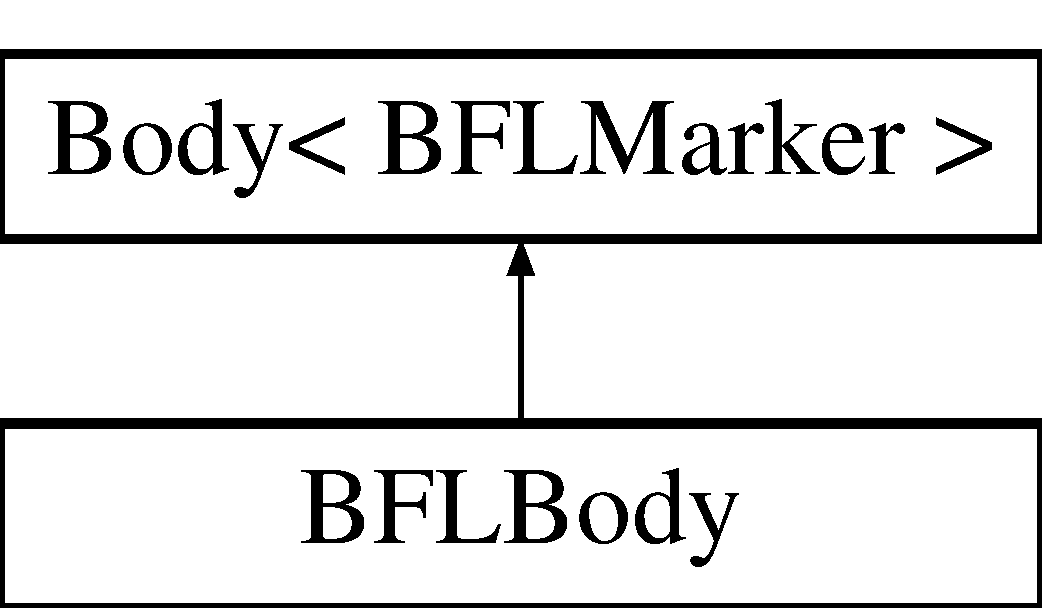
\includegraphics[height=2.000000cm]{class_b_f_l_body}
\end{center}
\end{figure}
\subsection*{Public Member Functions}
\begin{DoxyCompactItemize}
\item 
\hyperlink{class_b_f_l_body_ab7b3b9f55b59b977401bcf8dead8cfce}{B\+F\+L\+Body} (void)
\item 
\hyperlink{class_b_f_l_body_ad6d343eed8481d8b652261642e184c43}{$\sim$\+B\+F\+L\+Body} (void)
\item 
\hyperlink{class_b_f_l_body_a5dc2907ac609b0fb0a89347b4f66f2ca}{B\+F\+L\+Body} (\hyperlink{class_p_cpts}{P\+Cpts} $\ast$\+\_\+\+P\+Cpts, \hyperlink{class_grid_obj}{Grid\+Obj} $\ast$g\+\_\+hierarchy)
\end{DoxyCompactItemize}
\subsection*{Protected Member Functions}
\begin{DoxyCompactItemize}
\item 
void \hyperlink{class_b_f_l_body_ac220c45e09a037a1f8c596d09d71e3a0}{computeQ} (int i, int j, int k, int N\+\_\+lim, int M\+\_\+lim, int K\+\_\+lim, \hyperlink{class_grid_obj}{Grid\+Obj} $\ast$g)
\item 
void \hyperlink{class_b_f_l_body_a2c98a2521ad9c1a3831a6004f867a307}{computeQ} (int i, int j, int N\+\_\+lim, int M\+\_\+lim, \hyperlink{class_grid_obj}{Grid\+Obj} $\ast$g)
\end{DoxyCompactItemize}
\subsection*{Protected Attributes}
\begin{DoxyCompactItemize}
\item 
std\+::vector$<$ std\+::vector$<$ double $>$ $>$ \hyperlink{class_b_f_l_body_a77b97a6b61e16616ab718c56c3a34622}{Q}
\end{DoxyCompactItemize}
\subsection*{Friends}
\begin{DoxyCompactItemize}
\item 
class \hyperlink{class_b_f_l_body_a55cfec1721fb1b9d9e7592bd6288c998}{Grid\+Obj}
\end{DoxyCompactItemize}


\subsection{Constructor \& Destructor Documentation}
\index{B\+F\+L\+Body@{B\+F\+L\+Body}!B\+F\+L\+Body@{B\+F\+L\+Body}}
\index{B\+F\+L\+Body@{B\+F\+L\+Body}!B\+F\+L\+Body@{B\+F\+L\+Body}}
\subsubsection[{\texorpdfstring{B\+F\+L\+Body(void)}{BFLBody(void)}}]{\setlength{\rightskip}{0pt plus 5cm}B\+F\+L\+Body\+::\+B\+F\+L\+Body (
\begin{DoxyParamCaption}
\item[{void}]{}
\end{DoxyParamCaption}
)}\hypertarget{class_b_f_l_body_ab7b3b9f55b59b977401bcf8dead8cfce}{}\label{class_b_f_l_body_ab7b3b9f55b59b977401bcf8dead8cfce}
\index{B\+F\+L\+Body@{B\+F\+L\+Body}!````~B\+F\+L\+Body@{$\sim$\+B\+F\+L\+Body}}
\index{````~B\+F\+L\+Body@{$\sim$\+B\+F\+L\+Body}!B\+F\+L\+Body@{B\+F\+L\+Body}}
\subsubsection[{\texorpdfstring{$\sim$\+B\+F\+L\+Body(void)}{~BFLBody(void)}}]{\setlength{\rightskip}{0pt plus 5cm}B\+F\+L\+Body\+::$\sim$\+B\+F\+L\+Body (
\begin{DoxyParamCaption}
\item[{void}]{}
\end{DoxyParamCaption}
)}\hypertarget{class_b_f_l_body_ad6d343eed8481d8b652261642e184c43}{}\label{class_b_f_l_body_ad6d343eed8481d8b652261642e184c43}
\index{B\+F\+L\+Body@{B\+F\+L\+Body}!B\+F\+L\+Body@{B\+F\+L\+Body}}
\index{B\+F\+L\+Body@{B\+F\+L\+Body}!B\+F\+L\+Body@{B\+F\+L\+Body}}
\subsubsection[{\texorpdfstring{B\+F\+L\+Body(\+P\+Cpts $\ast$\+\_\+\+P\+Cpts, Grid\+Obj $\ast$g\+\_\+hierarchy)}{BFLBody(PCpts *_PCpts, GridObj *g_hierarchy)}}]{\setlength{\rightskip}{0pt plus 5cm}B\+F\+L\+Body\+::\+B\+F\+L\+Body (
\begin{DoxyParamCaption}
\item[{{\bf P\+Cpts} $\ast$}]{\+\_\+\+P\+Cpts, }
\item[{{\bf Grid\+Obj} $\ast$}]{g\+\_\+hierarchy}
\end{DoxyParamCaption}
)}\hypertarget{class_b_f_l_body_a5dc2907ac609b0fb0a89347b4f66f2ca}{}\label{class_b_f_l_body_a5dc2907ac609b0fb0a89347b4f66f2ca}


\subsection{Member Function Documentation}
\index{B\+F\+L\+Body@{B\+F\+L\+Body}!computeQ@{computeQ}}
\index{computeQ@{computeQ}!B\+F\+L\+Body@{B\+F\+L\+Body}}
\subsubsection[{\texorpdfstring{compute\+Q(int i, int j, int k, int N\+\_\+lim, int M\+\_\+lim, int K\+\_\+lim, Grid\+Obj $\ast$g)}{computeQ(int i, int j, int k, int N_lim, int M_lim, int K_lim, GridObj *g)}}]{\setlength{\rightskip}{0pt plus 5cm}void B\+F\+L\+Body\+::computeQ (
\begin{DoxyParamCaption}
\item[{int}]{i, }
\item[{int}]{j, }
\item[{int}]{k, }
\item[{int}]{N\+\_\+lim, }
\item[{int}]{M\+\_\+lim, }
\item[{int}]{K\+\_\+lim, }
\item[{{\bf Grid\+Obj} $\ast$}]{g}
\end{DoxyParamCaption}
)\hspace{0.3cm}{\ttfamily [protected]}}\hypertarget{class_b_f_l_body_ac220c45e09a037a1f8c596d09d71e3a0}{}\label{class_b_f_l_body_ac220c45e09a037a1f8c596d09d71e3a0}
\index{B\+F\+L\+Body@{B\+F\+L\+Body}!computeQ@{computeQ}}
\index{computeQ@{computeQ}!B\+F\+L\+Body@{B\+F\+L\+Body}}
\subsubsection[{\texorpdfstring{compute\+Q(int i, int j, int N\+\_\+lim, int M\+\_\+lim, Grid\+Obj $\ast$g)}{computeQ(int i, int j, int N_lim, int M_lim, GridObj *g)}}]{\setlength{\rightskip}{0pt plus 5cm}void B\+F\+L\+Body\+::computeQ (
\begin{DoxyParamCaption}
\item[{int}]{i, }
\item[{int}]{j, }
\item[{int}]{N\+\_\+lim, }
\item[{int}]{M\+\_\+lim, }
\item[{{\bf Grid\+Obj} $\ast$}]{g}
\end{DoxyParamCaption}
)\hspace{0.3cm}{\ttfamily [protected]}}\hypertarget{class_b_f_l_body_a2c98a2521ad9c1a3831a6004f867a307}{}\label{class_b_f_l_body_a2c98a2521ad9c1a3831a6004f867a307}


\subsection{Friends And Related Function Documentation}
\index{B\+F\+L\+Body@{B\+F\+L\+Body}!Grid\+Obj@{Grid\+Obj}}
\index{Grid\+Obj@{Grid\+Obj}!B\+F\+L\+Body@{B\+F\+L\+Body}}
\subsubsection[{\texorpdfstring{Grid\+Obj}{GridObj}}]{\setlength{\rightskip}{0pt plus 5cm}friend class {\bf Grid\+Obj}\hspace{0.3cm}{\ttfamily [friend]}}\hypertarget{class_b_f_l_body_a55cfec1721fb1b9d9e7592bd6288c998}{}\label{class_b_f_l_body_a55cfec1721fb1b9d9e7592bd6288c998}


\subsection{Member Data Documentation}
\index{B\+F\+L\+Body@{B\+F\+L\+Body}!Q@{Q}}
\index{Q@{Q}!B\+F\+L\+Body@{B\+F\+L\+Body}}
\subsubsection[{\texorpdfstring{Q}{Q}}]{\setlength{\rightskip}{0pt plus 5cm}std\+::vector$<$ std\+::vector$<$double$>$ $>$ B\+F\+L\+Body\+::Q\hspace{0.3cm}{\ttfamily [protected]}}\hypertarget{class_b_f_l_body_a77b97a6b61e16616ab718c56c3a34622}{}\label{class_b_f_l_body_a77b97a6b61e16616ab718c56c3a34622}


The documentation for this class was generated from the following files\+:\begin{DoxyCompactItemize}
\item 
\hyperlink{_b_f_l_body_8h}{B\+F\+L\+Body.\+h}\item 
\hyperlink{_b_f_l_body_8cpp}{B\+F\+L\+Body.\+cpp}\end{DoxyCompactItemize}

\hypertarget{class_b_f_l_marker}{}\section{B\+F\+L\+Marker Class Reference}
\label{class_b_f_l_marker}\index{B\+F\+L\+Marker@{B\+F\+L\+Marker}}


{\ttfamily \#include $<$B\+F\+L\+Marker.\+h$>$}

Inheritance diagram for B\+F\+L\+Marker\+:\begin{figure}[H]
\begin{center}
\leavevmode
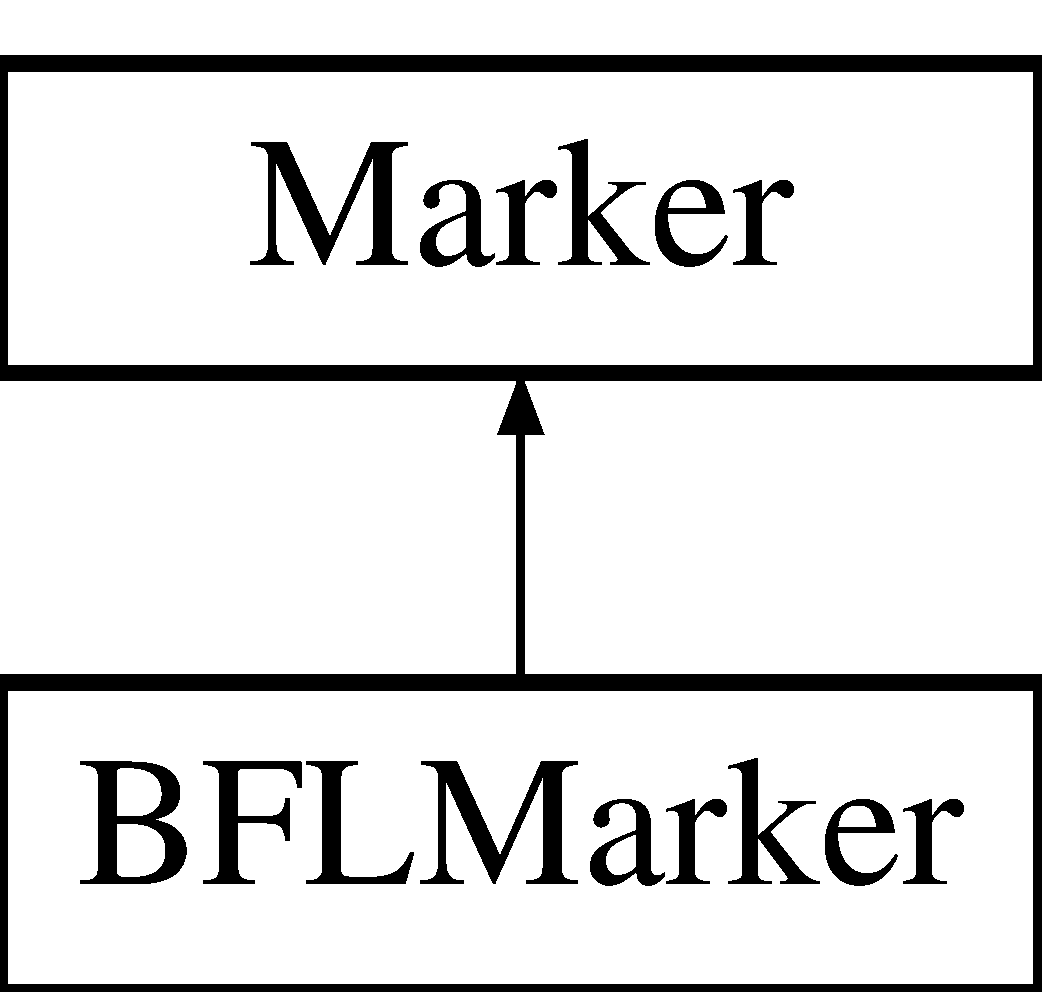
\includegraphics[height=2.000000cm]{class_b_f_l_marker}
\end{center}
\end{figure}
\subsection*{Public Member Functions}
\begin{DoxyCompactItemize}
\item 
\hyperlink{class_b_f_l_marker_a5d6b8e4b1cfac580b86aa0f3b2f22c24}{B\+F\+L\+Marker} (void)
\item 
\hyperlink{class_b_f_l_marker_a10ac169924a35ee14599992290540447}{$\sim$\+B\+F\+L\+Marker} (void)
\item 
\hyperlink{class_b_f_l_marker_a2ec501d3d93f2dbde8e56e6155ef3c09}{B\+F\+L\+Marker} (double x, double y, double z)
\end{DoxyCompactItemize}
\subsection*{Friends}
\begin{DoxyCompactItemize}
\item 
class \hyperlink{class_b_f_l_marker_a253e046b9808d9a35fda96a16d22edb3}{B\+F\+L\+Body}
\end{DoxyCompactItemize}
\subsection*{Additional Inherited Members}


\subsection{Constructor \& Destructor Documentation}
\index{B\+F\+L\+Marker@{B\+F\+L\+Marker}!B\+F\+L\+Marker@{B\+F\+L\+Marker}}
\index{B\+F\+L\+Marker@{B\+F\+L\+Marker}!B\+F\+L\+Marker@{B\+F\+L\+Marker}}
\subsubsection[{\texorpdfstring{B\+F\+L\+Marker(void)}{BFLMarker(void)}}]{\setlength{\rightskip}{0pt plus 5cm}B\+F\+L\+Marker\+::\+B\+F\+L\+Marker (
\begin{DoxyParamCaption}
\item[{void}]{}
\end{DoxyParamCaption}
)}\hypertarget{class_b_f_l_marker_a5d6b8e4b1cfac580b86aa0f3b2f22c24}{}\label{class_b_f_l_marker_a5d6b8e4b1cfac580b86aa0f3b2f22c24}
\index{B\+F\+L\+Marker@{B\+F\+L\+Marker}!````~B\+F\+L\+Marker@{$\sim$\+B\+F\+L\+Marker}}
\index{````~B\+F\+L\+Marker@{$\sim$\+B\+F\+L\+Marker}!B\+F\+L\+Marker@{B\+F\+L\+Marker}}
\subsubsection[{\texorpdfstring{$\sim$\+B\+F\+L\+Marker(void)}{~BFLMarker(void)}}]{\setlength{\rightskip}{0pt plus 5cm}B\+F\+L\+Marker\+::$\sim$\+B\+F\+L\+Marker (
\begin{DoxyParamCaption}
\item[{void}]{}
\end{DoxyParamCaption}
)}\hypertarget{class_b_f_l_marker_a10ac169924a35ee14599992290540447}{}\label{class_b_f_l_marker_a10ac169924a35ee14599992290540447}
\index{B\+F\+L\+Marker@{B\+F\+L\+Marker}!B\+F\+L\+Marker@{B\+F\+L\+Marker}}
\index{B\+F\+L\+Marker@{B\+F\+L\+Marker}!B\+F\+L\+Marker@{B\+F\+L\+Marker}}
\subsubsection[{\texorpdfstring{B\+F\+L\+Marker(double x, double y, double z)}{BFLMarker(double x, double y, double z)}}]{\setlength{\rightskip}{0pt plus 5cm}B\+F\+L\+Marker\+::\+B\+F\+L\+Marker (
\begin{DoxyParamCaption}
\item[{double}]{x, }
\item[{double}]{y, }
\item[{double}]{z}
\end{DoxyParamCaption}
)}\hypertarget{class_b_f_l_marker_a2ec501d3d93f2dbde8e56e6155ef3c09}{}\label{class_b_f_l_marker_a2ec501d3d93f2dbde8e56e6155ef3c09}


\subsection{Friends And Related Function Documentation}
\index{B\+F\+L\+Marker@{B\+F\+L\+Marker}!B\+F\+L\+Body@{B\+F\+L\+Body}}
\index{B\+F\+L\+Body@{B\+F\+L\+Body}!B\+F\+L\+Marker@{B\+F\+L\+Marker}}
\subsubsection[{\texorpdfstring{B\+F\+L\+Body}{BFLBody}}]{\setlength{\rightskip}{0pt plus 5cm}friend class {\bf B\+F\+L\+Body}\hspace{0.3cm}{\ttfamily [friend]}}\hypertarget{class_b_f_l_marker_a253e046b9808d9a35fda96a16d22edb3}{}\label{class_b_f_l_marker_a253e046b9808d9a35fda96a16d22edb3}


The documentation for this class was generated from the following files\+:\begin{DoxyCompactItemize}
\item 
\hyperlink{_b_f_l_marker_8h}{B\+F\+L\+Marker.\+h}\item 
\hyperlink{_b_f_l_marker_8cpp}{B\+F\+L\+Marker.\+cpp}\end{DoxyCompactItemize}

\hypertarget{class_body}{}\section{Body$<$ Marker\+Type $>$ Class Template Reference}
\label{class_body}\index{Body$<$ Marker\+Type $>$@{Body$<$ Marker\+Type $>$}}


Generic body class.  




{\ttfamily \#include $<$Body.\+h$>$}

\subsection*{Public Member Functions}
\begin{DoxyCompactItemize}
\item 
\hyperlink{class_body_a684a431c9215429149f36949ab007353}{Body} (void)
\begin{DoxyCompactList}\small\item\em Default Constructor. \end{DoxyCompactList}\item 
\hyperlink{class_body_a62fb64b91f20eeef2d454994bdbc8b37}{$\sim$\+Body} (void)
\begin{DoxyCompactList}\small\item\em Default destructor. \end{DoxyCompactList}\item 
\hyperlink{class_body_a939c580274ddf89d1a7e8c6b12ea70ca}{Body} (\hyperlink{class_grid_obj}{Grid\+Obj} $\ast$g)
\begin{DoxyCompactList}\small\item\em Custom constructor setting owning grid. \end{DoxyCompactList}\end{DoxyCompactItemize}
\subsection*{Protected Member Functions}
\begin{DoxyCompactItemize}
\item 
void \hyperlink{class_body_aa965f7b498528230aa2f56a9abf6bf06}{add\+Marker} (double x, double y, double z)
\begin{DoxyCompactList}\small\item\em Add marker to the body. \end{DoxyCompactList}\item 
\hyperlink{class_marker_data}{Marker\+Data} $\ast$ \hyperlink{class_body_aebc3c7911b4ad10b1f9853d3f5fc7514}{get\+Marker\+Data} (double x, double y, double z)
\begin{DoxyCompactList}\small\item\em Retrieve marker data. \end{DoxyCompactList}\item 
void \hyperlink{class_body_a3a1ba74da8020cc3ee7f4fffde0b4477}{marker\+Adder} (double x, double y, double z, int \&curr\+\_\+mark, std\+::vector$<$ int $>$ \&counter)
\begin{DoxyCompactList}\small\item\em Downsampling marker adding method. \end{DoxyCompactList}\item 
bool \hyperlink{class_body_aa7733bbcd85af5fa4e8822889fba7b33}{is\+In\+Voxel} (double x, double y, double z, int curr\+\_\+mark)
\begin{DoxyCompactList}\small\item\em Determines whether a point is inside another marker\textquotesingle{}s support voxel. \end{DoxyCompactList}\item 
bool \hyperlink{class_body_a3ed926c01461f32d64b4a5405e920e36}{is\+Voxel\+Marker\+Voxel} (double x, double y, double z)
\begin{DoxyCompactList}\small\item\em Determines whether a point is inside an existing marker\textquotesingle{}s support voxel. \end{DoxyCompactList}\end{DoxyCompactItemize}
\subsection*{Protected Attributes}
\begin{DoxyCompactItemize}
\item 
double \hyperlink{class_body_a1d4ac2e6fdbc946d5eab0973fd78770b}{spacing}
\begin{DoxyCompactList}\small\item\em Spacing of the markers in physical units. \end{DoxyCompactList}\item 
std\+::vector$<$ Marker\+Type $>$ \hyperlink{class_body_a4e0ac821f2331ec67793a44e36c855e3}{markers}
\begin{DoxyCompactList}\small\item\em Array of markers which make up the body. \end{DoxyCompactList}\item 
bool \hyperlink{class_body_a2701bdb00789d26ed72d6138d2e21bcb}{closed\+\_\+surface}
\begin{DoxyCompactList}\small\item\em Flag to specify whether or not it is a closed surface (for output) \end{DoxyCompactList}\item 
\hyperlink{class_grid_obj}{Grid\+Obj} $\ast$ \hyperlink{class_body_a5197f31e50222c32adefb795a93d7156}{\+\_\+\+Owner}
\begin{DoxyCompactList}\small\item\em Pointer to owning grid. \end{DoxyCompactList}\end{DoxyCompactItemize}


\subsection{Detailed Description}
\subsubsection*{template$<$typename Marker\+Type$>$\\*
class Body$<$ Marker\+Type $>$}

Generic body class. 

Can consist of any type of \hyperlink{class_marker}{Marker} so templated. 

\subsection{Constructor \& Destructor Documentation}
\index{Body@{Body}!Body@{Body}}
\index{Body@{Body}!Body@{Body}}
\subsubsection[{\texorpdfstring{Body(void)}{Body(void)}}]{\setlength{\rightskip}{0pt plus 5cm}template$<$typename Marker\+Type$>$ {\bf Body}$<$ Marker\+Type $>$\+::{\bf Body} (
\begin{DoxyParamCaption}
\item[{void}]{}
\end{DoxyParamCaption}
)\hspace{0.3cm}{\ttfamily [inline]}}\hypertarget{class_body_a684a431c9215429149f36949ab007353}{}\label{class_body_a684a431c9215429149f36949ab007353}


Default Constructor. 

\index{Body@{Body}!````~Body@{$\sim$\+Body}}
\index{````~Body@{$\sim$\+Body}!Body@{Body}}
\subsubsection[{\texorpdfstring{$\sim$\+Body(void)}{~Body(void)}}]{\setlength{\rightskip}{0pt plus 5cm}template$<$typename Marker\+Type$>$ {\bf Body}$<$ Marker\+Type $>$\+::$\sim${\bf Body} (
\begin{DoxyParamCaption}
\item[{void}]{}
\end{DoxyParamCaption}
)\hspace{0.3cm}{\ttfamily [inline]}}\hypertarget{class_body_a62fb64b91f20eeef2d454994bdbc8b37}{}\label{class_body_a62fb64b91f20eeef2d454994bdbc8b37}


Default destructor. 

\index{Body@{Body}!Body@{Body}}
\index{Body@{Body}!Body@{Body}}
\subsubsection[{\texorpdfstring{Body(\+Grid\+Obj $\ast$g)}{Body(GridObj *g)}}]{\setlength{\rightskip}{0pt plus 5cm}template$<$typename Marker\+Type$>$ {\bf Body}$<$ Marker\+Type $>$\+::{\bf Body} (
\begin{DoxyParamCaption}
\item[{{\bf Grid\+Obj} $\ast$}]{g}
\end{DoxyParamCaption}
)\hspace{0.3cm}{\ttfamily [inline]}}\hypertarget{class_body_a939c580274ddf89d1a7e8c6b12ea70ca}{}\label{class_body_a939c580274ddf89d1a7e8c6b12ea70ca}


Custom constructor setting owning grid. 


\begin{DoxyParams}{Parameters}
{\em g} & pointer to grid which owns this body. \\
\hline
\end{DoxyParams}


\subsection{Member Function Documentation}
\index{Body@{Body}!add\+Marker@{add\+Marker}}
\index{add\+Marker@{add\+Marker}!Body@{Body}}
\subsubsection[{\texorpdfstring{add\+Marker(double x, double y, double z)}{addMarker(double x, double y, double z)}}]{\setlength{\rightskip}{0pt plus 5cm}template$<$typename Marker\+Type$>$ void {\bf Body}$<$ Marker\+Type $>$\+::add\+Marker (
\begin{DoxyParamCaption}
\item[{double}]{x, }
\item[{double}]{y, }
\item[{double}]{z}
\end{DoxyParamCaption}
)\hspace{0.3cm}{\ttfamily [inline]}, {\ttfamily [protected]}}\hypertarget{class_body_aa965f7b498528230aa2f56a9abf6bf06}{}\label{class_body_aa965f7b498528230aa2f56a9abf6bf06}


Add marker to the body. 


\begin{DoxyParams}{Parameters}
{\em x} & X-\/position of marker. \\
\hline
{\em y} & Y-\/position of marker. \\
\hline
{\em z} & Z-\/position of marker. \\
\hline
\end{DoxyParams}
\index{Body@{Body}!get\+Marker\+Data@{get\+Marker\+Data}}
\index{get\+Marker\+Data@{get\+Marker\+Data}!Body@{Body}}
\subsubsection[{\texorpdfstring{get\+Marker\+Data(double x, double y, double z)}{getMarkerData(double x, double y, double z)}}]{\setlength{\rightskip}{0pt plus 5cm}template$<$typename Marker\+Type$>$ {\bf Marker\+Data}$\ast$ {\bf Body}$<$ Marker\+Type $>$\+::get\+Marker\+Data (
\begin{DoxyParamCaption}
\item[{double}]{x, }
\item[{double}]{y, }
\item[{double}]{z}
\end{DoxyParamCaption}
)\hspace{0.3cm}{\ttfamily [inline]}, {\ttfamily [protected]}}\hypertarget{class_body_aebc3c7911b4ad10b1f9853d3f5fc7514}{}\label{class_body_aebc3c7911b4ad10b1f9853d3f5fc7514}


Retrieve marker data. 

Return marker and voxel/primary support data associated with supplied global position.


\begin{DoxyParams}{Parameters}
{\em x} & X-\/position nearest to marker to be retrieved. \\
\hline
{\em y} & Y-\/position nearest to marker to be retrieved. \\
\hline
{\em z} & Z-\/position nearest to marker to be retrieved. \\
\hline
\end{DoxyParams}
\begin{DoxyReturn}{Returns}
\hyperlink{class_marker_data}{Marker\+Data} marker data structure returned. If no marker found, structure is marked as invalid. 
\end{DoxyReturn}
\index{Body@{Body}!is\+In\+Voxel@{is\+In\+Voxel}}
\index{is\+In\+Voxel@{is\+In\+Voxel}!Body@{Body}}
\subsubsection[{\texorpdfstring{is\+In\+Voxel(double x, double y, double z, int curr\+\_\+mark)}{isInVoxel(double x, double y, double z, int curr_mark)}}]{\setlength{\rightskip}{0pt plus 5cm}template$<$typename Marker\+Type$>$ bool {\bf Body}$<$ Marker\+Type $>$\+::is\+In\+Voxel (
\begin{DoxyParamCaption}
\item[{double}]{x, }
\item[{double}]{y, }
\item[{double}]{z, }
\item[{int}]{curr\+\_\+mark}
\end{DoxyParamCaption}
)\hspace{0.3cm}{\ttfamily [inline]}, {\ttfamily [protected]}}\hypertarget{class_body_aa7733bbcd85af5fa4e8822889fba7b33}{}\label{class_body_aa7733bbcd85af5fa4e8822889fba7b33}


Determines whether a point is inside another marker\textquotesingle{}s support voxel. 


\begin{DoxyParams}{Parameters}
{\em x} & X-\/position of point. \\
\hline
{\em y} & Y-\/position of point. \\
\hline
{\em z} & Z-\/position of point. \\
\hline
{\em curr\+\_\+mark} & ID of the marker. \\
\hline
\end{DoxyParams}
\begin{DoxyReturn}{Returns}
true of false 
\end{DoxyReturn}
\index{Body@{Body}!is\+Voxel\+Marker\+Voxel@{is\+Voxel\+Marker\+Voxel}}
\index{is\+Voxel\+Marker\+Voxel@{is\+Voxel\+Marker\+Voxel}!Body@{Body}}
\subsubsection[{\texorpdfstring{is\+Voxel\+Marker\+Voxel(double x, double y, double z)}{isVoxelMarkerVoxel(double x, double y, double z)}}]{\setlength{\rightskip}{0pt plus 5cm}template$<$typename Marker\+Type$>$ bool {\bf Body}$<$ Marker\+Type $>$\+::is\+Voxel\+Marker\+Voxel (
\begin{DoxyParamCaption}
\item[{double}]{x, }
\item[{double}]{y, }
\item[{double}]{z}
\end{DoxyParamCaption}
)\hspace{0.3cm}{\ttfamily [inline]}, {\ttfamily [protected]}}\hypertarget{class_body_a3ed926c01461f32d64b4a5405e920e36}{}\label{class_body_a3ed926c01461f32d64b4a5405e920e36}


Determines whether a point is inside an existing marker\textquotesingle{}s support voxel. 


\begin{DoxyParams}{Parameters}
{\em x} & X-\/position of point. \\
\hline
{\em y} & Y-\/position of point. \\
\hline
{\em z} & Z-\/position of point. \\
\hline
\end{DoxyParams}
\begin{DoxyReturn}{Returns}
true of false 
\end{DoxyReturn}
\index{Body@{Body}!marker\+Adder@{marker\+Adder}}
\index{marker\+Adder@{marker\+Adder}!Body@{Body}}
\subsubsection[{\texorpdfstring{marker\+Adder(double x, double y, double z, int \&curr\+\_\+mark, std\+::vector$<$ int $>$ \&counter)}{markerAdder(double x, double y, double z, int &curr_mark, std::vector< int > &counter)}}]{\setlength{\rightskip}{0pt plus 5cm}template$<$typename Marker\+Type$>$ void {\bf Body}$<$ Marker\+Type $>$\+::marker\+Adder (
\begin{DoxyParamCaption}
\item[{double}]{x, }
\item[{double}]{y, }
\item[{double}]{z, }
\item[{int \&}]{curr\+\_\+mark, }
\item[{std\+::vector$<$ int $>$ \&}]{counter}
\end{DoxyParamCaption}
)\hspace{0.3cm}{\ttfamily [inline]}, {\ttfamily [protected]}}\hypertarget{class_body_a3a1ba74da8020cc3ee7f4fffde0b4477}{}\label{class_body_a3a1ba74da8020cc3ee7f4fffde0b4477}


Downsampling marker adding method. 

This method tries to add a marker to body at the location given but obeys the rules of a voxel-\/grid filter to ensure markers are distributed such that their spacing roughly matches the background lattice.


\begin{DoxyParams}{Parameters}
{\em x} & desired X-\/position of new marker. \\
\hline
{\em y} & desired Y-\/position of new marker. \\
\hline
{\em z} & desired Z-\/position of new marker. \\
\hline
{\em curr\+\_\+mark} & is a reference to the ID of last marker. \\
\hline
{\em counter} & is a reference to the total number of markers in the body. \\
\hline
\end{DoxyParams}


\subsection{Member Data Documentation}
\index{Body@{Body}!\+\_\+\+Owner@{\+\_\+\+Owner}}
\index{\+\_\+\+Owner@{\+\_\+\+Owner}!Body@{Body}}
\subsubsection[{\texorpdfstring{\+\_\+\+Owner}{_Owner}}]{\setlength{\rightskip}{0pt plus 5cm}template$<$typename Marker\+Type$>$ {\bf Grid\+Obj}$\ast$ {\bf Body}$<$ Marker\+Type $>$\+::\+\_\+\+Owner\hspace{0.3cm}{\ttfamily [protected]}}\hypertarget{class_body_a5197f31e50222c32adefb795a93d7156}{}\label{class_body_a5197f31e50222c32adefb795a93d7156}


Pointer to owning grid. 

\index{Body@{Body}!closed\+\_\+surface@{closed\+\_\+surface}}
\index{closed\+\_\+surface@{closed\+\_\+surface}!Body@{Body}}
\subsubsection[{\texorpdfstring{closed\+\_\+surface}{closed_surface}}]{\setlength{\rightskip}{0pt plus 5cm}template$<$typename Marker\+Type$>$ bool {\bf Body}$<$ Marker\+Type $>$\+::closed\+\_\+surface\hspace{0.3cm}{\ttfamily [protected]}}\hypertarget{class_body_a2701bdb00789d26ed72d6138d2e21bcb}{}\label{class_body_a2701bdb00789d26ed72d6138d2e21bcb}


Flag to specify whether or not it is a closed surface (for output) 

\index{Body@{Body}!markers@{markers}}
\index{markers@{markers}!Body@{Body}}
\subsubsection[{\texorpdfstring{markers}{markers}}]{\setlength{\rightskip}{0pt plus 5cm}template$<$typename Marker\+Type$>$ std\+::vector$<$Marker\+Type$>$ {\bf Body}$<$ Marker\+Type $>$\+::markers\hspace{0.3cm}{\ttfamily [protected]}}\hypertarget{class_body_a4e0ac821f2331ec67793a44e36c855e3}{}\label{class_body_a4e0ac821f2331ec67793a44e36c855e3}


Array of markers which make up the body. 

\index{Body@{Body}!spacing@{spacing}}
\index{spacing@{spacing}!Body@{Body}}
\subsubsection[{\texorpdfstring{spacing}{spacing}}]{\setlength{\rightskip}{0pt plus 5cm}template$<$typename Marker\+Type$>$ double {\bf Body}$<$ Marker\+Type $>$\+::spacing\hspace{0.3cm}{\ttfamily [protected]}}\hypertarget{class_body_a1d4ac2e6fdbc946d5eab0973fd78770b}{}\label{class_body_a1d4ac2e6fdbc946d5eab0973fd78770b}


Spacing of the markers in physical units. 



The documentation for this class was generated from the following file\+:\begin{DoxyCompactItemize}
\item 
\hyperlink{_body_8h}{Body.\+h}\end{DoxyCompactItemize}

\hypertarget{struct_mpi_manager_1_1buffer__struct}{}\section{Mpi\+Manager\+:\+:buffer\+\_\+struct Struct Reference}
\label{struct_mpi_manager_1_1buffer__struct}\index{Mpi\+Manager\+::buffer\+\_\+struct@{Mpi\+Manager\+::buffer\+\_\+struct}}


Structure storing buffers sizes in each direction for particular grid.  




{\ttfamily \#include $<$Mpi\+Manager.\+h$>$}

\subsection*{Public Attributes}
\begin{DoxyCompactItemize}
\item 
int \hyperlink{struct_mpi_manager_1_1buffer__struct_aea0037fce808f601ae9c1e48926dbd0e}{size} \mbox{[}\hyperlink{definitions_8h_a3310be18f0cfda9ca2a17c51518a97e9}{L\+\_\+\+M\+P\+I\+\_\+dir}\mbox{]}
\begin{DoxyCompactList}\small\item\em Buffer sizes for each direction. \end{DoxyCompactList}\item 
int \hyperlink{struct_mpi_manager_1_1buffer__struct_adc6bb3b15665e3fb5834e6134395e1f9}{level}
\begin{DoxyCompactList}\small\item\em Grid level. \end{DoxyCompactList}\item 
int \hyperlink{struct_mpi_manager_1_1buffer__struct_a81730a85a03630880e8c378fcb8d3298}{region}
\begin{DoxyCompactList}\small\item\em Region number. \end{DoxyCompactList}\end{DoxyCompactItemize}


\subsection{Detailed Description}
Structure storing buffers sizes in each direction for particular grid. 

\subsection{Member Data Documentation}
\index{Mpi\+Manager\+::buffer\+\_\+struct@{Mpi\+Manager\+::buffer\+\_\+struct}!level@{level}}
\index{level@{level}!Mpi\+Manager\+::buffer\+\_\+struct@{Mpi\+Manager\+::buffer\+\_\+struct}}
\subsubsection[{\texorpdfstring{level}{level}}]{\setlength{\rightskip}{0pt plus 5cm}int Mpi\+Manager\+::buffer\+\_\+struct\+::level}\hypertarget{struct_mpi_manager_1_1buffer__struct_adc6bb3b15665e3fb5834e6134395e1f9}{}\label{struct_mpi_manager_1_1buffer__struct_adc6bb3b15665e3fb5834e6134395e1f9}


Grid level. 

\index{Mpi\+Manager\+::buffer\+\_\+struct@{Mpi\+Manager\+::buffer\+\_\+struct}!region@{region}}
\index{region@{region}!Mpi\+Manager\+::buffer\+\_\+struct@{Mpi\+Manager\+::buffer\+\_\+struct}}
\subsubsection[{\texorpdfstring{region}{region}}]{\setlength{\rightskip}{0pt plus 5cm}int Mpi\+Manager\+::buffer\+\_\+struct\+::region}\hypertarget{struct_mpi_manager_1_1buffer__struct_a81730a85a03630880e8c378fcb8d3298}{}\label{struct_mpi_manager_1_1buffer__struct_a81730a85a03630880e8c378fcb8d3298}


Region number. 

\index{Mpi\+Manager\+::buffer\+\_\+struct@{Mpi\+Manager\+::buffer\+\_\+struct}!size@{size}}
\index{size@{size}!Mpi\+Manager\+::buffer\+\_\+struct@{Mpi\+Manager\+::buffer\+\_\+struct}}
\subsubsection[{\texorpdfstring{size}{size}}]{\setlength{\rightskip}{0pt plus 5cm}int Mpi\+Manager\+::buffer\+\_\+struct\+::size\mbox{[}{\bf L\+\_\+\+M\+P\+I\+\_\+dir}\mbox{]}}\hypertarget{struct_mpi_manager_1_1buffer__struct_aea0037fce808f601ae9c1e48926dbd0e}{}\label{struct_mpi_manager_1_1buffer__struct_aea0037fce808f601ae9c1e48926dbd0e}


Buffer sizes for each direction. 



The documentation for this struct was generated from the following file\+:\begin{DoxyCompactItemize}
\item 
\hyperlink{_mpi_manager_8h}{Mpi\+Manager.\+h}\end{DoxyCompactItemize}

\hypertarget{class_grid_obj}{}\section{Grid\+Obj Class Reference}
\label{class_grid_obj}\index{Grid\+Obj@{Grid\+Obj}}


Grid class.  




{\ttfamily \#include $<$Grid\+Obj.\+h$>$}

\subsection*{Public Member Functions}
\begin{DoxyCompactItemize}
\item 
\hyperlink{class_grid_obj_acc3416599b59236e87b6b60a07e678af}{Grid\+Obj} ()
\begin{DoxyCompactList}\small\item\em Default Constructor. \end{DoxyCompactList}\item 
\hyperlink{class_grid_obj_aaadde3417da5f31e1b8b33635487b56e}{Grid\+Obj} (int \hyperlink{class_grid_obj_a7dfedc4442a386ec15c8b03ca899c1a9}{level})
\begin{DoxyCompactList}\small\item\em Serial build constructor for top level grid. \end{DoxyCompactList}\item 
\hyperlink{class_grid_obj_a40600a8b8a286b8299bca8265b62f51b}{Grid\+Obj} (int Region\+Number, \hyperlink{class_grid_obj}{Grid\+Obj} \&p\+Grid)
\begin{DoxyCompactList}\small\item\em Constructor for a sub-\/grid. \end{DoxyCompactList}\item 
\hyperlink{class_grid_obj_a9ea61d35cb51f7f7f454da9e9b5b0bac}{Grid\+Obj} (int \hyperlink{class_grid_obj_a7dfedc4442a386ec15c8b03ca899c1a9}{level}, std\+::vector$<$ int $>$ local\+\_\+size, std\+::vector$<$ std\+::vector$<$ double $>$ $>$ Global\+Lims\+Pos)
\begin{DoxyCompactList}\small\item\em M\+PI constructor for top level grid. \end{DoxyCompactList}\item 
\hyperlink{class_grid_obj_ace563099d85c330ac48f35b515422522}{$\sim$\+Grid\+Obj} ()
\begin{DoxyCompactList}\small\item\em Default Destructor. \end{DoxyCompactList}\item 
void \hyperlink{class_grid_obj_aa8041f7344af6cf9732199aa107fdbc6}{L\+B\+M\+\_\+init\+Velocity} ()
\begin{DoxyCompactList}\small\item\em Method to initialise the lattice velocity. \end{DoxyCompactList}\item 
void \hyperlink{class_grid_obj_aac0e8a3fe74c69b3308ef3e19100f95c}{L\+B\+M\+\_\+init\+Rho} ()
\begin{DoxyCompactList}\small\item\em Method to initialise the lattice density. \end{DoxyCompactList}\item 
void \hyperlink{class_grid_obj_aeea74cc13001620abec1ba819233f714}{L\+B\+M\+\_\+init\+Grid} ()
\begin{DoxyCompactList}\small\item\em Wrapper to initialise all L0 lattice quantities. \end{DoxyCompactList}\item 
void \hyperlink{class_grid_obj_afbaf6155b26acb6a21dcf7be68520607}{L\+B\+M\+\_\+init\+Grid} (std\+::vector$<$ int $>$ local\+\_\+size, std\+::vector$<$ std\+::vector$<$ double $>$ $>$ Global\+Lims\+Pos)
\begin{DoxyCompactList}\small\item\em Method to initialise all L0 lattice quantities. \end{DoxyCompactList}\item 
void \hyperlink{class_grid_obj_a697f4d7fc6c9ed18e609528847b1e175}{L\+B\+M\+\_\+init\+Sub\+Grid} (\hyperlink{class_grid_obj}{Grid\+Obj} \&p\+Grid)
\begin{DoxyCompactList}\small\item\em Method to initialise all sub-\/grid quantities. \end{DoxyCompactList}\item 
void \hyperlink{class_grid_obj_a7a4c2d4eb5bc8f312d0998a55b38f0e2}{L\+B\+M\+\_\+init\+Grid\+To\+Grid\+Mappings} (\hyperlink{class_grid_obj}{Grid\+Obj} \&p\+Grid)
\begin{DoxyCompactList}\small\item\em Method to initialise the mapping parameters between this grid and the supplied parent. \end{DoxyCompactList}\item 
void \hyperlink{class_grid_obj_a32da287cacc2cbd15c3cee482ea4b010}{L\+B\+M\+\_\+init\+Position\+Vector} (double start\+\_\+pos, double end\+\_\+pos, \hyperlink{stdafx_8h_afbad8e4a2f1e9903755b1bd2fe8273cf}{e\+Cartesian\+Direction} dir)
\begin{DoxyCompactList}\small\item\em Method to initialise the position vector on the grid between the start and end positions supplied. \end{DoxyCompactList}\item 
void \hyperlink{class_grid_obj_a4b6edceeda49496365e725eb67931961}{L\+B\+M\+\_\+init\+Bound\+Lab} ()
\begin{DoxyCompactList}\small\item\em Method to initialise wall and object labels on L0. \end{DoxyCompactList}\item 
void \hyperlink{class_grid_obj_a5dd08730d7cdea576bb4b337786a9bcf}{L\+B\+M\+\_\+init\+Solid\+Lab} ()
\begin{DoxyCompactList}\small\item\em Method to initialise label-\/based solids. \end{DoxyCompactList}\item 
void \hyperlink{class_grid_obj_a3ba133d06625fb576ca0909b946033b2}{L\+B\+M\+\_\+init\+Refined\+Lab} (\hyperlink{class_grid_obj}{Grid\+Obj} \&p\+Grid)
\begin{DoxyCompactList}\small\item\em Method to initialise all labels on sub-\/grids. \end{DoxyCompactList}\item 
void \hyperlink{class_grid_obj_a023713976673d029103690a91c5415f9}{L\+B\+M\+\_\+init\+\_\+get\+Inlet\+Profile} ()
\begin{DoxyCompactList}\small\item\em Method to import an input profile from a file. \end{DoxyCompactList}\item 
void \hyperlink{class_grid_obj_ac4ca0327a53171fe8e1c3076e9f1353f}{L\+B\+M\+\_\+kbc\+Collide} (int i, int j, int k, \hyperlink{class_i_vector}{I\+Vector}$<$ double $>$ \&f\+\_\+new)
\begin{DoxyCompactList}\small\item\em K\+BC collision operator. \end{DoxyCompactList}\item 
void \hyperlink{class_grid_obj_ab69942450175d12c75f4b8d33b06c905}{L\+B\+M\+\_\+macro} (int i, int j, int k)
\begin{DoxyCompactList}\small\item\em Site-\/specific macroscopic update. \end{DoxyCompactList}\item 
void \hyperlink{class_grid_obj_a5701631be6333e512c7fc8dd6ecabf85}{L\+B\+M\+\_\+reset\+Forces} ()
\begin{DoxyCompactList}\small\item\em Method to reset body forces. \end{DoxyCompactList}\item 
\hyperlink{stdafx_8h_ac1e8a42306d8e67cb94ca31c3956ee78}{D\+E\+P\+R\+E\+C\+A\+T\+ED} void \hyperlink{class_grid_obj_a2dc94b1d2e3f14a1a086b8bfa078839b}{bc\+\_\+apply\+Bounce\+Back} (int label, int i, int j, int k)
\begin{DoxyCompactList}\small\item\em Method to apply half-\/way bounce-\/back. \end{DoxyCompactList}\item 
\hyperlink{stdafx_8h_ac1e8a42306d8e67cb94ca31c3956ee78}{D\+E\+P\+R\+E\+C\+A\+T\+ED} void \hyperlink{class_grid_obj_ae1d63a43d1dee6c7b25880c8a9bb97c9}{bc\+\_\+apply\+Spec\+Reflect} (int label, int i, int j, int k)
\begin{DoxyCompactList}\small\item\em Method to apply half-\/way specular reflection. \end{DoxyCompactList}\item 
\hyperlink{stdafx_8h_ac1e8a42306d8e67cb94ca31c3956ee78}{D\+E\+P\+R\+E\+C\+A\+T\+ED} void \hyperlink{class_grid_obj_a5602705b2575b09e27dd0065de3542f6}{bc\+\_\+apply\+Regularised} (int label, int i, int j, int k)
\begin{DoxyCompactList}\small\item\em Method to apply regularised velocity inlet. \end{DoxyCompactList}\item 
\hyperlink{stdafx_8h_ac1e8a42306d8e67cb94ca31c3956ee78}{D\+E\+P\+R\+E\+C\+A\+T\+ED} void \hyperlink{class_grid_obj_a385c4803f4803e380a520ac9b3dcb31d}{bc\+\_\+apply\+Extrapolation} (int label, int i, int j, int k)
\begin{DoxyCompactList}\small\item\em Method to apply extrapolation outlet. \end{DoxyCompactList}\item 
\hyperlink{stdafx_8h_ac1e8a42306d8e67cb94ca31c3956ee78}{D\+E\+P\+R\+E\+C\+A\+T\+ED} void \hyperlink{class_grid_obj_aeff3b54617b7ae65f08c96e653f9035f}{bc\+\_\+apply\+Bfl} (int i, int j, int k)
\begin{DoxyCompactList}\small\item\em Method to apply B\+FL bounce-\/back. \end{DoxyCompactList}\item 
\hyperlink{stdafx_8h_ac1e8a42306d8e67cb94ca31c3956ee78}{D\+E\+P\+R\+E\+C\+A\+T\+ED} void \hyperlink{class_grid_obj_ae4fd999e7334c8ec8e1118c92e0c7338}{bc\+\_\+apply\+Nrbc} (int i, int j, int k)
\begin{DoxyCompactList}\small\item\em Method to apply N\+R\+BC. \end{DoxyCompactList}\item 
void \hyperlink{class_grid_obj_ab0d47be7ccafaa84b5d43da69e2082b9}{L\+B\+M\+\_\+add\+Sub\+Grid} (int Region\+Number)
\begin{DoxyCompactList}\small\item\em Wrapper method to add sub-\/grid to this grid. \end{DoxyCompactList}\item 
void \hyperlink{class_grid_obj_a1f334215b7789ea1ad8e2d1e15c67fb2}{io\+\_\+textout} (std\+::string output\+\_\+tag)
\begin{DoxyCompactList}\small\item\em Verbose A\+S\+C\+II writer. \end{DoxyCompactList}\item 
void \hyperlink{class_grid_obj_aa80aecb06d7a420865c32b8acc15581e}{io\+\_\+fgaout} ()
\begin{DoxyCompactList}\small\item\em .fga file writer. \end{DoxyCompactList}\item 
void \hyperlink{class_grid_obj_a94551d2e383da4b2a2c930488d436a42}{io\+\_\+restart} (\hyperlink{_grid_obj_8h_ad1926c22ad82853adff44c4b76b97827}{e\+I\+O\+Flag} I\+O\+\_\+flag)
\begin{DoxyCompactList}\small\item\em Restart file read-\/writer. \end{DoxyCompactList}\item 
void \hyperlink{class_grid_obj_af7e8782f95d15884d761cc4f1d5926c0}{io\+\_\+probe\+Output} ()
\begin{DoxyCompactList}\small\item\em Probe writer. \end{DoxyCompactList}\item 
void \hyperlink{class_grid_obj_acf311bbf350fd48104663eaabebca835}{io\+\_\+lite} (double tval, std\+::string Tag)
\begin{DoxyCompactList}\small\item\em A\+S\+C\+II dump of grid data. \end{DoxyCompactList}\item 
int \hyperlink{class_grid_obj_adc960ac818748b839e81d1375782caa7}{io\+\_\+hdf5} (double tval)
\begin{DoxyCompactList}\small\item\em H\+D\+F5 writer. \end{DoxyCompactList}\item 
void \hyperlink{class_grid_obj_ac65e9a1a8aa854d25281780d6b52665b}{L\+B\+M\+\_\+multi\+\_\+opt} (int subcycle=0)
\begin{DoxyCompactList}\small\item\em Optimised L\+BM multi-\/grid kernel. \end{DoxyCompactList}\end{DoxyCompactItemize}
\subsection*{Public Attributes}
\begin{DoxyCompactItemize}
\item 
std\+::vector$<$ double $>$ \hyperlink{class_grid_obj_af31df133bf9419da6222a0dbb4e54bab}{X\+Pos}
\begin{DoxyCompactList}\small\item\em Vector of global X positions of each site. \end{DoxyCompactList}\item 
std\+::vector$<$ double $>$ \hyperlink{class_grid_obj_a2bd4e9b575377b8e76e5ebe7a3a31194}{Y\+Pos}
\begin{DoxyCompactList}\small\item\em Vector of global Y positions of each site. \end{DoxyCompactList}\item 
std\+::vector$<$ double $>$ \hyperlink{class_grid_obj_af859d35bf0a03cee8965ce3e22e651c6}{Z\+Pos}
\begin{DoxyCompactList}\small\item\em Vector of global Z positions of each site. \end{DoxyCompactList}\item 
\hyperlink{class_i_vector}{I\+Vector}$<$ \hyperlink{_grid_obj_8h_a12f8ec8f0e7a4584b9fe481bb53fa60e}{e\+Type} $>$ \hyperlink{class_grid_obj_a8ce077fba648f767361039eb924c45ae}{Lat\+Typ}
\begin{DoxyCompactList}\small\item\em Flattened 3D array of site labels. \end{DoxyCompactList}\item 
double \hyperlink{class_grid_obj_a4efe4f79d600da2f459a0cc08b89b40c}{dh}
\begin{DoxyCompactList}\small\item\em Physical lattice spacing (same for x, y and z) \end{DoxyCompactList}\item 
int \hyperlink{class_grid_obj_ae0b724f2d977cfe38df2bb191e2fb042}{region\+\_\+number}
\begin{DoxyCompactList}\small\item\em Region number. \end{DoxyCompactList}\item 
int \hyperlink{class_grid_obj_a7dfedc4442a386ec15c8b03ca899c1a9}{level}
\begin{DoxyCompactList}\small\item\em Level in embedded grid hierarchy. \end{DoxyCompactList}\item 
double \hyperlink{class_grid_obj_afd504b39f12eb0a237bc6313de94e094}{dt}
\begin{DoxyCompactList}\small\item\em Physical time step size. \end{DoxyCompactList}\item 
int \hyperlink{class_grid_obj_a783b18a053e244ae7b7b436ab21c0592}{t}
\begin{DoxyCompactList}\small\item\em Number of completed iterations on this level. \end{DoxyCompactList}\item 
double \hyperlink{class_grid_obj_a755f85eb5480d959211e00937a478ae9}{nu}
\begin{DoxyCompactList}\small\item\em Kinematic viscosity (in lattice units) \end{DoxyCompactList}\item 
double \hyperlink{class_grid_obj_a21461e5d39c5ae83ae42170c829e9da3}{omega}
\begin{DoxyCompactList}\small\item\em Relaxation frequency. \end{DoxyCompactList}\item 
double \hyperlink{class_grid_obj_a147cfb80b653ca4432432e8185cf38ef}{timeav\+\_\+mpi\+\_\+overhead}
\begin{DoxyCompactList}\small\item\em Time-\/averaged time of M\+PI communication. \end{DoxyCompactList}\item 
double \hyperlink{class_grid_obj_a2ad670e6b9bdd28b5060397800170310}{timeav\+\_\+timestep}
\begin{DoxyCompactList}\small\item\em Time-\/averaged time of a timestep. \end{DoxyCompactList}\item 
int \hyperlink{class_grid_obj_a5eb35752a7c0741510975d9ee6aa3ce1}{N\+\_\+lim}
\begin{DoxyCompactList}\small\item\em Local size of grid in X-\/direction. \end{DoxyCompactList}\item 
int \hyperlink{class_grid_obj_a01d3f362634c896ecdb80f0e6304c12f}{M\+\_\+lim}
\begin{DoxyCompactList}\small\item\em Local size of grid in Y-\/direction. \end{DoxyCompactList}\item 
int \hyperlink{class_grid_obj_aaccc404f2fbdbaef8c5dd134f7d9e17f}{K\+\_\+lim}
\begin{DoxyCompactList}\small\item\em Local size of grid in Z-\/direction. \end{DoxyCompactList}\item 
double \hyperlink{class_grid_obj_adcd2bcbd5bb4009d7c84097e1356a1fa}{X\+Origin}
\begin{DoxyCompactList}\small\item\em Position of grid left edge. \end{DoxyCompactList}\item 
double \hyperlink{class_grid_obj_a30c070fe26def1366db2b3e66b3cd29d}{Y\+Origin}
\begin{DoxyCompactList}\small\item\em Position of grid bottom edge. \end{DoxyCompactList}\item 
double \hyperlink{class_grid_obj_a69d43fd31ba7edd4fc9f02eb0c0fcefd}{Z\+Origin}
\begin{DoxyCompactList}\small\item\em Position of grid front edge. \end{DoxyCompactList}\end{DoxyCompactItemize}
\subsection*{Friends}
\begin{DoxyCompactItemize}
\item 
class \hyperlink{class_grid_obj_a831466b4226dde3791b04756e4cfa6fc}{Mpi\+Manager}
\item 
class \hyperlink{class_grid_obj_a8b86bdcdb7c54a536293d8632363e114}{Object\+Manager}
\item 
class \hyperlink{class_grid_obj_a8891d532b9568ad83535721b0e6b79c9}{Grid\+Utils}
\end{DoxyCompactItemize}


\subsection{Detailed Description}
Grid class. 

This class represents a grid (lattice) and is capable of owning a nested hierarchy of child grids. 

\subsection{Constructor \& Destructor Documentation}
\index{Grid\+Obj@{Grid\+Obj}!Grid\+Obj@{Grid\+Obj}}
\index{Grid\+Obj@{Grid\+Obj}!Grid\+Obj@{Grid\+Obj}}
\subsubsection[{\texorpdfstring{Grid\+Obj()}{GridObj()}}]{\setlength{\rightskip}{0pt plus 5cm}Grid\+Obj\+::\+Grid\+Obj (
\begin{DoxyParamCaption}
\item[{void}]{}
\end{DoxyParamCaption}
)}\hypertarget{class_grid_obj_acc3416599b59236e87b6b60a07e678af}{}\label{class_grid_obj_acc3416599b59236e87b6b60a07e678af}


Default Constructor. 

\index{Grid\+Obj@{Grid\+Obj}!Grid\+Obj@{Grid\+Obj}}
\index{Grid\+Obj@{Grid\+Obj}!Grid\+Obj@{Grid\+Obj}}
\subsubsection[{\texorpdfstring{Grid\+Obj(int level)}{GridObj(int level)}}]{\setlength{\rightskip}{0pt plus 5cm}Grid\+Obj\+::\+Grid\+Obj (
\begin{DoxyParamCaption}
\item[{int}]{level}
\end{DoxyParamCaption}
)}\hypertarget{class_grid_obj_aaadde3417da5f31e1b8b33635487b56e}{}\label{class_grid_obj_aaadde3417da5f31e1b8b33635487b56e}


Serial build constructor for top level grid. 

Coarse limits are set to zero and then L0-\/specific initialiser called.


\begin{DoxyParams}{Parameters}
{\em level} & always should be zero as top level grid. \\
\hline
\end{DoxyParams}
\index{Grid\+Obj@{Grid\+Obj}!Grid\+Obj@{Grid\+Obj}}
\index{Grid\+Obj@{Grid\+Obj}!Grid\+Obj@{Grid\+Obj}}
\subsubsection[{\texorpdfstring{Grid\+Obj(int Region\+Number, Grid\+Obj \&p\+Grid)}{GridObj(int RegionNumber, GridObj &pGrid)}}]{\setlength{\rightskip}{0pt plus 5cm}Grid\+Obj\+::\+Grid\+Obj (
\begin{DoxyParamCaption}
\item[{int}]{Region\+Number, }
\item[{{\bf Grid\+Obj} \&}]{p\+Grid}
\end{DoxyParamCaption}
)}\hypertarget{class_grid_obj_a40600a8b8a286b8299bca8265b62f51b}{}\label{class_grid_obj_a40600a8b8a286b8299bca8265b62f51b}


Constructor for a sub-\/grid. 

This is not called directly but by the add\+Sub\+Grid() method which first performs a check to see if a sub-\/grid is required.


\begin{DoxyParams}{Parameters}
{\em Region\+Number} & ID indicating the region of nested refinement to which this sub-\/grid belongs. \\
\hline
{\em p\+Grid} & pointer to parent grid. \\
\hline
\end{DoxyParams}
\index{Grid\+Obj@{Grid\+Obj}!Grid\+Obj@{Grid\+Obj}}
\index{Grid\+Obj@{Grid\+Obj}!Grid\+Obj@{Grid\+Obj}}
\subsubsection[{\texorpdfstring{Grid\+Obj(int level, std\+::vector$<$ int $>$ local\+\_\+size, std\+::vector$<$ std\+::vector$<$ double $>$ $>$ Global\+Lims\+Pos)}{GridObj(int level, std::vector< int > local_size, std::vector< std::vector< double > > GlobalLimsPos)}}]{\setlength{\rightskip}{0pt plus 5cm}Grid\+Obj\+::\+Grid\+Obj (
\begin{DoxyParamCaption}
\item[{int}]{level, }
\item[{std\+::vector$<$ int $>$}]{local\+\_\+size, }
\item[{std\+::vector$<$ std\+::vector$<$ double $>$ $>$}]{Global\+Lims\+Pos}
\end{DoxyParamCaption}
)}\hypertarget{class_grid_obj_a9ea61d35cb51f7f7f454da9e9b5b0bac}{}\label{class_grid_obj_a9ea61d35cb51f7f7f454da9e9b5b0bac}


M\+PI constructor for top level grid. 

When using M\+PI, this constructors a local grid which represents an appropriate portion of the top-\/level grid as dictated by the extent of this rank.


\begin{DoxyParams}{Parameters}
{\em level} & always should be zero as top level grid. \\
\hline
{\em local\+\_\+size} & vector indicating dimensions of local grid including halo. \\
\hline
{\em Global\+Lims\+Pos} & vector indicating the global positions of the edges of this local grid core as held by the \hyperlink{class_mpi_manager}{Mpi\+Manager}. \\
\hline
\end{DoxyParams}
\index{Grid\+Obj@{Grid\+Obj}!````~Grid\+Obj@{$\sim$\+Grid\+Obj}}
\index{````~Grid\+Obj@{$\sim$\+Grid\+Obj}!Grid\+Obj@{Grid\+Obj}}
\subsubsection[{\texorpdfstring{$\sim$\+Grid\+Obj()}{~GridObj()}}]{\setlength{\rightskip}{0pt plus 5cm}Grid\+Obj\+::$\sim$\+Grid\+Obj (
\begin{DoxyParamCaption}
\item[{void}]{}
\end{DoxyParamCaption}
)}\hypertarget{class_grid_obj_ace563099d85c330ac48f35b515422522}{}\label{class_grid_obj_ace563099d85c330ac48f35b515422522}


Default Destructor. 



\subsection{Member Function Documentation}
\index{Grid\+Obj@{Grid\+Obj}!bc\+\_\+apply\+Bfl@{bc\+\_\+apply\+Bfl}}
\index{bc\+\_\+apply\+Bfl@{bc\+\_\+apply\+Bfl}!Grid\+Obj@{Grid\+Obj}}
\subsubsection[{\texorpdfstring{bc\+\_\+apply\+Bfl(int i, int j, int k)}{bc_applyBfl(int i, int j, int k)}}]{\setlength{\rightskip}{0pt plus 5cm}void Grid\+Obj\+::bc\+\_\+apply\+Bfl (
\begin{DoxyParamCaption}
\item[{int}]{i, }
\item[{int}]{j, }
\item[{int}]{k}
\end{DoxyParamCaption}
)}\hypertarget{class_grid_obj_aeff3b54617b7ae65f08c96e653f9035f}{}\label{class_grid_obj_aeff3b54617b7ae65f08c96e653f9035f}


Method to apply B\+FL bounce-\/back. 

Currently, assumes only 1 B\+FL body present on the grid.


\begin{DoxyParams}{Parameters}
{\em i} & current site i-\/index. \\
\hline
{\em j} & current site j-\/index. \\
\hline
{\em k} & current site k-\/index. \\
\hline
\end{DoxyParams}
\index{Grid\+Obj@{Grid\+Obj}!bc\+\_\+apply\+Bounce\+Back@{bc\+\_\+apply\+Bounce\+Back}}
\index{bc\+\_\+apply\+Bounce\+Back@{bc\+\_\+apply\+Bounce\+Back}!Grid\+Obj@{Grid\+Obj}}
\subsubsection[{\texorpdfstring{bc\+\_\+apply\+Bounce\+Back(int label, int i, int j, int k)}{bc_applyBounceBack(int label, int i, int j, int k)}}]{\setlength{\rightskip}{0pt plus 5cm}void Grid\+Obj\+::bc\+\_\+apply\+Bounce\+Back (
\begin{DoxyParamCaption}
\item[{int}]{label, }
\item[{int}]{i, }
\item[{int}]{j, }
\item[{int}]{k}
\end{DoxyParamCaption}
)}\hypertarget{class_grid_obj_a2dc94b1d2e3f14a1a086b8bfa078839b}{}\label{class_grid_obj_a2dc94b1d2e3f14a1a086b8bfa078839b}


Method to apply half-\/way bounce-\/back. 


\begin{DoxyParams}{Parameters}
{\em label} & current site label. \\
\hline
{\em i} & current site i-\/index. \\
\hline
{\em j} & current site j-\/index. \\
\hline
{\em k} & current site k-\/index. \\
\hline
\end{DoxyParams}
\index{Grid\+Obj@{Grid\+Obj}!bc\+\_\+apply\+Extrapolation@{bc\+\_\+apply\+Extrapolation}}
\index{bc\+\_\+apply\+Extrapolation@{bc\+\_\+apply\+Extrapolation}!Grid\+Obj@{Grid\+Obj}}
\subsubsection[{\texorpdfstring{bc\+\_\+apply\+Extrapolation(int label, int i, int j, int k)}{bc_applyExtrapolation(int label, int i, int j, int k)}}]{\setlength{\rightskip}{0pt plus 5cm}void Grid\+Obj\+::bc\+\_\+apply\+Extrapolation (
\begin{DoxyParamCaption}
\item[{int}]{label, }
\item[{int}]{i, }
\item[{int}]{j, }
\item[{int}]{k}
\end{DoxyParamCaption}
)}\hypertarget{class_grid_obj_a385c4803f4803e380a520ac9b3dcb31d}{}\label{class_grid_obj_a385c4803f4803e380a520ac9b3dcb31d}


Method to apply extrapolation outlet. 

Can only be applied on right-\/hand wall.


\begin{DoxyParams}{Parameters}
{\em label} & current site label. \\
\hline
{\em i} & current site i-\/index. \\
\hline
{\em j} & current site j-\/index. \\
\hline
{\em k} & current site k-\/index. \\
\hline
\end{DoxyParams}
\index{Grid\+Obj@{Grid\+Obj}!bc\+\_\+apply\+Nrbc@{bc\+\_\+apply\+Nrbc}}
\index{bc\+\_\+apply\+Nrbc@{bc\+\_\+apply\+Nrbc}!Grid\+Obj@{Grid\+Obj}}
\subsubsection[{\texorpdfstring{bc\+\_\+apply\+Nrbc(int i, int j, int k)}{bc_applyNrbc(int i, int j, int k)}}]{\setlength{\rightskip}{0pt plus 5cm}void Grid\+Obj\+::bc\+\_\+apply\+Nrbc (
\begin{DoxyParamCaption}
\item[{int}]{i, }
\item[{int}]{j, }
\item[{int}]{k}
\end{DoxyParamCaption}
)}\hypertarget{class_grid_obj_ae4fd999e7334c8ec8e1118c92e0c7338}{}\label{class_grid_obj_ae4fd999e7334c8ec8e1118c92e0c7338}


Method to apply N\+R\+BC. 

Not implemented in this version.


\begin{DoxyParams}{Parameters}
{\em i} & current site i-\/index. \\
\hline
{\em j} & current site j-\/index. \\
\hline
{\em k} & current site k-\/index. \\
\hline
\end{DoxyParams}
\index{Grid\+Obj@{Grid\+Obj}!bc\+\_\+apply\+Regularised@{bc\+\_\+apply\+Regularised}}
\index{bc\+\_\+apply\+Regularised@{bc\+\_\+apply\+Regularised}!Grid\+Obj@{Grid\+Obj}}
\subsubsection[{\texorpdfstring{bc\+\_\+apply\+Regularised(int label, int i, int j, int k)}{bc_applyRegularised(int label, int i, int j, int k)}}]{\setlength{\rightskip}{0pt plus 5cm}void Grid\+Obj\+::bc\+\_\+apply\+Regularised (
\begin{DoxyParamCaption}
\item[{int}]{label, }
\item[{int}]{i, }
\item[{int}]{j, }
\item[{int}]{k}
\end{DoxyParamCaption}
)}\hypertarget{class_grid_obj_a5602705b2575b09e27dd0065de3542f6}{}\label{class_grid_obj_a5602705b2575b09e27dd0065de3542f6}


Method to apply regularised velocity inlet. 

Can be applied on any wall.


\begin{DoxyParams}{Parameters}
{\em label} & current site label. \\
\hline
{\em i} & current site i-\/index. \\
\hline
{\em j} & current site j-\/index. \\
\hline
{\em k} & current site k-\/index. \\
\hline
\end{DoxyParams}
\index{Grid\+Obj@{Grid\+Obj}!bc\+\_\+apply\+Spec\+Reflect@{bc\+\_\+apply\+Spec\+Reflect}}
\index{bc\+\_\+apply\+Spec\+Reflect@{bc\+\_\+apply\+Spec\+Reflect}!Grid\+Obj@{Grid\+Obj}}
\subsubsection[{\texorpdfstring{bc\+\_\+apply\+Spec\+Reflect(int label, int i, int j, int k)}{bc_applySpecReflect(int label, int i, int j, int k)}}]{\setlength{\rightskip}{0pt plus 5cm}void Grid\+Obj\+::bc\+\_\+apply\+Spec\+Reflect (
\begin{DoxyParamCaption}
\item[{int}]{label, }
\item[{int}]{i, }
\item[{int}]{j, }
\item[{int}]{k}
\end{DoxyParamCaption}
)}\hypertarget{class_grid_obj_ae1d63a43d1dee6c7b25880c8a9bb97c9}{}\label{class_grid_obj_ae1d63a43d1dee6c7b25880c8a9bb97c9}


Method to apply half-\/way specular reflection. 

Symmetry boundary condition for free-\/slip walls.


\begin{DoxyParams}{Parameters}
{\em label} & current site label. \\
\hline
{\em i} & current site i-\/index. \\
\hline
{\em j} & current site j-\/index. \\
\hline
{\em k} & current site k-\/index. \\
\hline
\end{DoxyParams}
\index{Grid\+Obj@{Grid\+Obj}!io\+\_\+fgaout@{io\+\_\+fgaout}}
\index{io\+\_\+fgaout@{io\+\_\+fgaout}!Grid\+Obj@{Grid\+Obj}}
\subsubsection[{\texorpdfstring{io\+\_\+fgaout()}{io_fgaout()}}]{\setlength{\rightskip}{0pt plus 5cm}void Grid\+Obj\+::io\+\_\+fgaout (
\begin{DoxyParamCaption}
{}
\end{DoxyParamCaption}
)}\hypertarget{class_grid_obj_aa80aecb06d7a420865c32b8acc15581e}{}\label{class_grid_obj_aa80aecb06d7a420865c32b8acc15581e}


.fga file writer. 

Writes the components of the macroscopic velocity of the grid at time t and call recursively for any sub-\/grid. Writes the data of each subgrid in a different .fga file. .fga is the A\+S\+C\+II file format used by Unreal Engine 4 to read the data that populates a Vector\+Field object. It doesn\textquotesingle{}t do anything if the model is not 2D or 3D. Since .fga files can only store 3D data \index{Grid\+Obj@{Grid\+Obj}!io\+\_\+hdf5@{io\+\_\+hdf5}}
\index{io\+\_\+hdf5@{io\+\_\+hdf5}!Grid\+Obj@{Grid\+Obj}}
\subsubsection[{\texorpdfstring{io\+\_\+hdf5(double tval)}{io_hdf5(double tval)}}]{\setlength{\rightskip}{0pt plus 5cm}int Grid\+Obj\+::io\+\_\+hdf5 (
\begin{DoxyParamCaption}
\item[{double}]{tval}
\end{DoxyParamCaption}
)}\hypertarget{class_grid_obj_adc960ac818748b839e81d1375782caa7}{}\label{class_grid_obj_adc960ac818748b839e81d1375782caa7}


H\+D\+F5 writer. 

Useful grid quantities written out as scalar arrays. Creates one $\ast$.h5 file per grid and data is grouped into timesteps within each file. Should be used with the merge tool at post-\/processing to conver to sructured V\+TK output readable in paraview.


\begin{DoxyParams}{Parameters}
{\em tval} & time value being written out. \\
\hline
\end{DoxyParams}
\index{Grid\+Obj@{Grid\+Obj}!io\+\_\+lite@{io\+\_\+lite}}
\index{io\+\_\+lite@{io\+\_\+lite}!Grid\+Obj@{Grid\+Obj}}
\subsubsection[{\texorpdfstring{io\+\_\+lite(double tval, std\+::string Tag)}{io_lite(double tval, std::string Tag)}}]{\setlength{\rightskip}{0pt plus 5cm}void Grid\+Obj\+::io\+\_\+lite (
\begin{DoxyParamCaption}
\item[{double}]{tval, }
\item[{std\+::string}]{T\+AG}
\end{DoxyParamCaption}
)}\hypertarget{class_grid_obj_acf311bbf350fd48104663eaabebca835}{}\label{class_grid_obj_acf311bbf350fd48104663eaabebca835}


A\+S\+C\+II dump of grid data. 

Generic A\+S\+C\+II writer for each rank to write out all grid data in rows into a single, unsorted file.


\begin{DoxyParams}{Parameters}
{\em tval} & time value being written out. \\
\hline
{\em T\+AG} & text identifier for the data. \\
\hline
\end{DoxyParams}
\index{Grid\+Obj@{Grid\+Obj}!io\+\_\+probe\+Output@{io\+\_\+probe\+Output}}
\index{io\+\_\+probe\+Output@{io\+\_\+probe\+Output}!Grid\+Obj@{Grid\+Obj}}
\subsubsection[{\texorpdfstring{io\+\_\+probe\+Output()}{io_probeOutput()}}]{\setlength{\rightskip}{0pt plus 5cm}void Grid\+Obj\+::io\+\_\+probe\+Output (
\begin{DoxyParamCaption}
{}
\end{DoxyParamCaption}
)}\hypertarget{class_grid_obj_af7e8782f95d15884d761cc4f1d5926c0}{}\label{class_grid_obj_af7e8782f95d15884d761cc4f1d5926c0}


Probe writer. 

This routine writes the quantities at the probe locations to a single file. \index{Grid\+Obj@{Grid\+Obj}!io\+\_\+restart@{io\+\_\+restart}}
\index{io\+\_\+restart@{io\+\_\+restart}!Grid\+Obj@{Grid\+Obj}}
\subsubsection[{\texorpdfstring{io\+\_\+restart(e\+I\+O\+Flag I\+O\+\_\+flag)}{io_restart(eIOFlag IO_flag)}}]{\setlength{\rightskip}{0pt plus 5cm}void Grid\+Obj\+::io\+\_\+restart (
\begin{DoxyParamCaption}
\item[{{\bf e\+I\+O\+Flag}}]{I\+O\+\_\+flag}
\end{DoxyParamCaption}
)}\hypertarget{class_grid_obj_a94551d2e383da4b2a2c930488d436a42}{}\label{class_grid_obj_a94551d2e383da4b2a2c930488d436a42}


Restart file read-\/writer. 

This routine writes/reads the current rank\textquotesingle{}s data in the custom restart file format. If the file already exists, data is appended. IB body data are also written out but no other body information at present.


\begin{DoxyParams}{Parameters}
{\em I\+O\+\_\+flag} & flag to indicate whether a write or read \\
\hline
\end{DoxyParams}
\index{Grid\+Obj@{Grid\+Obj}!io\+\_\+textout@{io\+\_\+textout}}
\index{io\+\_\+textout@{io\+\_\+textout}!Grid\+Obj@{Grid\+Obj}}
\subsubsection[{\texorpdfstring{io\+\_\+textout(std\+::string output\+\_\+tag)}{io_textout(std::string output_tag)}}]{\setlength{\rightskip}{0pt plus 5cm}void Grid\+Obj\+::io\+\_\+textout (
\begin{DoxyParamCaption}
\item[{std\+::string}]{output\+\_\+tag}
\end{DoxyParamCaption}
)}\hypertarget{class_grid_obj_a1f334215b7789ea1ad8e2d1e15c67fb2}{}\label{class_grid_obj_a1f334215b7789ea1ad8e2d1e15c67fb2}


Verbose A\+S\+C\+II writer. 

Writes all the contents of the grid class at time t and call recursviely for any sub-\/grids. Writes to text file \char`\"{}\+Grids.\+out\char`\"{} by default.


\begin{DoxyParams}{Parameters}
{\em output\+\_\+tag} & text string added to top of output for identification. \\
\hline
\end{DoxyParams}
\index{Grid\+Obj@{Grid\+Obj}!L\+B\+M\+\_\+add\+Sub\+Grid@{L\+B\+M\+\_\+add\+Sub\+Grid}}
\index{L\+B\+M\+\_\+add\+Sub\+Grid@{L\+B\+M\+\_\+add\+Sub\+Grid}!Grid\+Obj@{Grid\+Obj}}
\subsubsection[{\texorpdfstring{L\+B\+M\+\_\+add\+Sub\+Grid(int Region\+Number)}{LBM_addSubGrid(int RegionNumber)}}]{\setlength{\rightskip}{0pt plus 5cm}void Grid\+Obj\+::\+L\+B\+M\+\_\+add\+Sub\+Grid (
\begin{DoxyParamCaption}
\item[{int}]{Region\+Number}
\end{DoxyParamCaption}
)}\hypertarget{class_grid_obj_ab0d47be7ccafaa84b5d43da69e2082b9}{}\label{class_grid_obj_ab0d47be7ccafaa84b5d43da69e2082b9}


Wrapper method to add sub-\/grid to this grid. 


\begin{DoxyParams}{Parameters}
{\em Region\+Number} & ID indicating the region of nested refinement to which this sub-\/grid belongs. \\
\hline
\end{DoxyParams}
\index{Grid\+Obj@{Grid\+Obj}!L\+B\+M\+\_\+init\+\_\+get\+Inlet\+Profile@{L\+B\+M\+\_\+init\+\_\+get\+Inlet\+Profile}}
\index{L\+B\+M\+\_\+init\+\_\+get\+Inlet\+Profile@{L\+B\+M\+\_\+init\+\_\+get\+Inlet\+Profile}!Grid\+Obj@{Grid\+Obj}}
\subsubsection[{\texorpdfstring{L\+B\+M\+\_\+init\+\_\+get\+Inlet\+Profile()}{LBM_init_getInletProfile()}}]{\setlength{\rightskip}{0pt plus 5cm}void Grid\+Obj\+::\+L\+B\+M\+\_\+init\+\_\+get\+Inlet\+Profile (
\begin{DoxyParamCaption}
{}
\end{DoxyParamCaption}
)}\hypertarget{class_grid_obj_a023713976673d029103690a91c5415f9}{}\label{class_grid_obj_a023713976673d029103690a91c5415f9}


Method to import an input profile from a file. 

Input data may be over-\/ or under-\/sampled but it must span the physical dimensions of the inlet otherwise the software does not known how to scale the data to fit. Inlet profile is always assumed to be oriented vertically (y-\/direction). \index{Grid\+Obj@{Grid\+Obj}!L\+B\+M\+\_\+init\+Bound\+Lab@{L\+B\+M\+\_\+init\+Bound\+Lab}}
\index{L\+B\+M\+\_\+init\+Bound\+Lab@{L\+B\+M\+\_\+init\+Bound\+Lab}!Grid\+Obj@{Grid\+Obj}}
\subsubsection[{\texorpdfstring{L\+B\+M\+\_\+init\+Bound\+Lab()}{LBM_initBoundLab()}}]{\setlength{\rightskip}{0pt plus 5cm}void Grid\+Obj\+::\+L\+B\+M\+\_\+init\+Bound\+Lab (
\begin{DoxyParamCaption}
{}
\end{DoxyParamCaption}
)}\hypertarget{class_grid_obj_a4b6edceeda49496365e725eb67931961}{}\label{class_grid_obj_a4b6edceeda49496365e725eb67931961}


Method to initialise wall and object labels on L0. 

The virtual wind tunnel definitions are implemented by this method. \index{Grid\+Obj@{Grid\+Obj}!L\+B\+M\+\_\+init\+Grid@{L\+B\+M\+\_\+init\+Grid}}
\index{L\+B\+M\+\_\+init\+Grid@{L\+B\+M\+\_\+init\+Grid}!Grid\+Obj@{Grid\+Obj}}
\subsubsection[{\texorpdfstring{L\+B\+M\+\_\+init\+Grid()}{LBM_initGrid()}}]{\setlength{\rightskip}{0pt plus 5cm}void Grid\+Obj\+::\+L\+B\+M\+\_\+init\+Grid (
\begin{DoxyParamCaption}
{}
\end{DoxyParamCaption}
)}\hypertarget{class_grid_obj_aeea74cc13001620abec1ba819233f714}{}\label{class_grid_obj_aeea74cc13001620abec1ba819233f714}


Wrapper to initialise all L0 lattice quantities. 

This method wraps the M\+P\+I-\/specific version. It is called by the serial build and sets the M\+P\+I-\/specific arguments to default values before calling the full initialiser. \index{Grid\+Obj@{Grid\+Obj}!L\+B\+M\+\_\+init\+Grid@{L\+B\+M\+\_\+init\+Grid}}
\index{L\+B\+M\+\_\+init\+Grid@{L\+B\+M\+\_\+init\+Grid}!Grid\+Obj@{Grid\+Obj}}
\subsubsection[{\texorpdfstring{L\+B\+M\+\_\+init\+Grid(std\+::vector$<$ int $>$ local\+\_\+size, std\+::vector$<$ std\+::vector$<$ double $>$ $>$ Global\+Lims\+Pos)}{LBM_initGrid(std::vector< int > local_size, std::vector< std::vector< double > > GlobalLimsPos)}}]{\setlength{\rightskip}{0pt plus 5cm}void Grid\+Obj\+::\+L\+B\+M\+\_\+init\+Grid (
\begin{DoxyParamCaption}
\item[{std\+::vector$<$ int $>$}]{local\+\_\+size, }
\item[{std\+::vector$<$ std\+::vector$<$ double $>$ $>$}]{rank\+\_\+core\+\_\+edge}
\end{DoxyParamCaption}
)}\hypertarget{class_grid_obj_afbaf6155b26acb6a21dcf7be68520607}{}\label{class_grid_obj_afbaf6155b26acb6a21dcf7be68520607}


Method to initialise all L0 lattice quantities. 


\begin{DoxyParams}{Parameters}
{\em local\+\_\+size} & local grid size on this rank including halo. \\
\hline
{\em rank\+\_\+core\+\_\+edge} & absolute positions of the rank edges (excludes overlapping halo). \\
\hline
\end{DoxyParams}
\index{Grid\+Obj@{Grid\+Obj}!L\+B\+M\+\_\+init\+Grid\+To\+Grid\+Mappings@{L\+B\+M\+\_\+init\+Grid\+To\+Grid\+Mappings}}
\index{L\+B\+M\+\_\+init\+Grid\+To\+Grid\+Mappings@{L\+B\+M\+\_\+init\+Grid\+To\+Grid\+Mappings}!Grid\+Obj@{Grid\+Obj}}
\subsubsection[{\texorpdfstring{L\+B\+M\+\_\+init\+Grid\+To\+Grid\+Mappings(\+Grid\+Obj \&p\+Grid)}{LBM_initGridToGridMappings(GridObj &pGrid)}}]{\setlength{\rightskip}{0pt plus 5cm}void Grid\+Obj\+::\+L\+B\+M\+\_\+init\+Grid\+To\+Grid\+Mappings (
\begin{DoxyParamCaption}
\item[{{\bf Grid\+Obj} \&}]{p\+Grid}
\end{DoxyParamCaption}
)}\hypertarget{class_grid_obj_a7a4c2d4eb5bc8f312d0998a55b38f0e2}{}\label{class_grid_obj_a7a4c2d4eb5bc8f312d0998a55b38f0e2}


Method to initialise the mapping parameters between this grid and the supplied parent. 

The mappings computed by this method are local ijk references to allow correct coupling during multi-\/grid operations.


\begin{DoxyParams}{Parameters}
{\em p\+Grid} & reference to parent grid. \\
\hline
\end{DoxyParams}
\index{Grid\+Obj@{Grid\+Obj}!L\+B\+M\+\_\+init\+Position\+Vector@{L\+B\+M\+\_\+init\+Position\+Vector}}
\index{L\+B\+M\+\_\+init\+Position\+Vector@{L\+B\+M\+\_\+init\+Position\+Vector}!Grid\+Obj@{Grid\+Obj}}
\subsubsection[{\texorpdfstring{L\+B\+M\+\_\+init\+Position\+Vector(double start\+\_\+pos, double end\+\_\+pos, e\+Cartesian\+Direction dir)}{LBM_initPositionVector(double start_pos, double end_pos, eCartesianDirection dir)}}]{\setlength{\rightskip}{0pt plus 5cm}void Grid\+Obj\+::\+L\+B\+M\+\_\+init\+Position\+Vector (
\begin{DoxyParamCaption}
\item[{double}]{start\+\_\+pos, }
\item[{double}]{end\+\_\+pos, }
\item[{{\bf e\+Cartesian\+Direction}}]{dir}
\end{DoxyParamCaption}
)}\hypertarget{class_grid_obj_a32da287cacc2cbd15c3cee482ea4b010}{}\label{class_grid_obj_a32da287cacc2cbd15c3cee482ea4b010}


Method to initialise the position vector on the grid between the start and end positions supplied. 

This method can be used for either serial or parallel initialisation as the halo and any wrap around is automatically taken into consideration. As such, the start position can be after the end position and the resulting vector will wrap at the correct point.


\begin{DoxyParams}{Parameters}
{\em start\+\_\+pos} & position of the first voxel centre in the vector. \\
\hline
{\em end\+\_\+pos} & position of the last voxel centre in the vector. \\
\hline
{\em dir} & direction of the vector. \\
\hline
\end{DoxyParams}
\index{Grid\+Obj@{Grid\+Obj}!L\+B\+M\+\_\+init\+Refined\+Lab@{L\+B\+M\+\_\+init\+Refined\+Lab}}
\index{L\+B\+M\+\_\+init\+Refined\+Lab@{L\+B\+M\+\_\+init\+Refined\+Lab}!Grid\+Obj@{Grid\+Obj}}
\subsubsection[{\texorpdfstring{L\+B\+M\+\_\+init\+Refined\+Lab(\+Grid\+Obj \&p\+Grid)}{LBM_initRefinedLab(GridObj &pGrid)}}]{\setlength{\rightskip}{0pt plus 5cm}void Grid\+Obj\+::\+L\+B\+M\+\_\+init\+Refined\+Lab (
\begin{DoxyParamCaption}
\item[{{\bf Grid\+Obj} \&}]{p\+Grid}
\end{DoxyParamCaption}
)}\hypertarget{class_grid_obj_a3ba133d06625fb576ca0909b946033b2}{}\label{class_grid_obj_a3ba133d06625fb576ca0909b946033b2}


Method to initialise all labels on sub-\/grids. 

Boundary labels are set by considering parent labels on overlapping sites and then assigning child labels appropriately.


\begin{DoxyParams}{Parameters}
{\em p\+Grid} & reference to parent grid. \\
\hline
\end{DoxyParams}
\index{Grid\+Obj@{Grid\+Obj}!L\+B\+M\+\_\+init\+Rho@{L\+B\+M\+\_\+init\+Rho}}
\index{L\+B\+M\+\_\+init\+Rho@{L\+B\+M\+\_\+init\+Rho}!Grid\+Obj@{Grid\+Obj}}
\subsubsection[{\texorpdfstring{L\+B\+M\+\_\+init\+Rho()}{LBM_initRho()}}]{\setlength{\rightskip}{0pt plus 5cm}void Grid\+Obj\+::\+L\+B\+M\+\_\+init\+Rho (
\begin{DoxyParamCaption}
{}
\end{DoxyParamCaption}
)}\hypertarget{class_grid_obj_aac0e8a3fe74c69b3308ef3e19100f95c}{}\label{class_grid_obj_aac0e8a3fe74c69b3308ef3e19100f95c}


Method to initialise the lattice density. 

\index{Grid\+Obj@{Grid\+Obj}!L\+B\+M\+\_\+init\+Solid\+Lab@{L\+B\+M\+\_\+init\+Solid\+Lab}}
\index{L\+B\+M\+\_\+init\+Solid\+Lab@{L\+B\+M\+\_\+init\+Solid\+Lab}!Grid\+Obj@{Grid\+Obj}}
\subsubsection[{\texorpdfstring{L\+B\+M\+\_\+init\+Solid\+Lab()}{LBM_initSolidLab()}}]{\setlength{\rightskip}{0pt plus 5cm}void Grid\+Obj\+::\+L\+B\+M\+\_\+init\+Solid\+Lab (
\begin{DoxyParamCaption}
{}
\end{DoxyParamCaption}
)}\hypertarget{class_grid_obj_a5dd08730d7cdea576bb4b337786a9bcf}{}\label{class_grid_obj_a5dd08730d7cdea576bb4b337786a9bcf}


Method to initialise label-\/based solids. 

\index{Grid\+Obj@{Grid\+Obj}!L\+B\+M\+\_\+init\+Sub\+Grid@{L\+B\+M\+\_\+init\+Sub\+Grid}}
\index{L\+B\+M\+\_\+init\+Sub\+Grid@{L\+B\+M\+\_\+init\+Sub\+Grid}!Grid\+Obj@{Grid\+Obj}}
\subsubsection[{\texorpdfstring{L\+B\+M\+\_\+init\+Sub\+Grid(\+Grid\+Obj \&p\+Grid)}{LBM_initSubGrid(GridObj &pGrid)}}]{\setlength{\rightskip}{0pt plus 5cm}void Grid\+Obj\+::\+L\+B\+M\+\_\+init\+Sub\+Grid (
\begin{DoxyParamCaption}
\item[{{\bf Grid\+Obj} \&}]{p\+Grid}
\end{DoxyParamCaption}
)}\hypertarget{class_grid_obj_a697f4d7fc6c9ed18e609528847b1e175}{}\label{class_grid_obj_a697f4d7fc6c9ed18e609528847b1e175}


Method to initialise all sub-\/grid quantities. 


\begin{DoxyParams}{Parameters}
{\em p\+Grid} & reference to parent grid. \\
\hline
\end{DoxyParams}
\index{Grid\+Obj@{Grid\+Obj}!L\+B\+M\+\_\+init\+Velocity@{L\+B\+M\+\_\+init\+Velocity}}
\index{L\+B\+M\+\_\+init\+Velocity@{L\+B\+M\+\_\+init\+Velocity}!Grid\+Obj@{Grid\+Obj}}
\subsubsection[{\texorpdfstring{L\+B\+M\+\_\+init\+Velocity()}{LBM_initVelocity()}}]{\setlength{\rightskip}{0pt plus 5cm}void Grid\+Obj\+::\+L\+B\+M\+\_\+init\+Velocity (
\begin{DoxyParamCaption}
{}
\end{DoxyParamCaption}
)}\hypertarget{class_grid_obj_aa8041f7344af6cf9732199aa107fdbc6}{}\label{class_grid_obj_aa8041f7344af6cf9732199aa107fdbc6}


Method to initialise the lattice velocity. 

Unless the L\+\_\+\+N\+O\+\_\+\+F\+L\+OW macro is defined, the initial velocity everywhere will be set to the values specified in the definitions file. \index{Grid\+Obj@{Grid\+Obj}!L\+B\+M\+\_\+kbc\+Collide@{L\+B\+M\+\_\+kbc\+Collide}}
\index{L\+B\+M\+\_\+kbc\+Collide@{L\+B\+M\+\_\+kbc\+Collide}!Grid\+Obj@{Grid\+Obj}}
\subsubsection[{\texorpdfstring{L\+B\+M\+\_\+kbc\+Collide(int i, int j, int k, I\+Vector$<$ double $>$ \&f\+\_\+new)}{LBM_kbcCollide(int i, int j, int k, IVector< double > &f_new)}}]{\setlength{\rightskip}{0pt plus 5cm}void Grid\+Obj\+::\+L\+B\+M\+\_\+kbc\+Collide (
\begin{DoxyParamCaption}
\item[{int}]{i, }
\item[{int}]{j, }
\item[{int}]{k, }
\item[{{\bf I\+Vector}$<$ double $>$ \&}]{f\+\_\+new}
\end{DoxyParamCaption}
)}\hypertarget{class_grid_obj_ac4ca0327a53171fe8e1c3076e9f1353f}{}\label{class_grid_obj_ac4ca0327a53171fe8e1c3076e9f1353f}


K\+BC collision operator. 

Applies K\+BC collision operator using the K\+B\+C-\/\+N4 and K\+B\+C-\/D models in 3D and 2D, respectively.


\begin{DoxyParams}{Parameters}
{\em i} & i-\/index of lattice site. \\
\hline
{\em j} & j-\/index of lattice site. \\
\hline
{\em k} & k-\/index of lattice site. \\
\hline
{\em f\+\_\+new} & reference to the temporary, post-\/collision grid. \\
\hline
\end{DoxyParams}
\index{Grid\+Obj@{Grid\+Obj}!L\+B\+M\+\_\+macro@{L\+B\+M\+\_\+macro}}
\index{L\+B\+M\+\_\+macro@{L\+B\+M\+\_\+macro}!Grid\+Obj@{Grid\+Obj}}
\subsubsection[{\texorpdfstring{L\+B\+M\+\_\+macro(int i, int j, int k)}{LBM_macro(int i, int j, int k)}}]{\setlength{\rightskip}{0pt plus 5cm}void Grid\+Obj\+::\+L\+B\+M\+\_\+macro (
\begin{DoxyParamCaption}
\item[{int}]{i, }
\item[{int}]{j, }
\item[{int}]{k}
\end{DoxyParamCaption}
)}\hypertarget{class_grid_obj_ab69942450175d12c75f4b8d33b06c905}{}\label{class_grid_obj_ab69942450175d12c75f4b8d33b06c905}


Site-\/specific macroscopic update. 

Overload of macroscopic quantity calculation to allow it to be applied to a single site as used by the M\+PI unpacking routine to update the values for the next collision step. This routine does not update the time-\/averaged quantities.


\begin{DoxyParams}{Parameters}
{\em i} & i-\/index of lattice site. \\
\hline
{\em j} & j-\/index of lattice site. \\
\hline
{\em k} & k-\/index of lattice site. \\
\hline
\end{DoxyParams}
\index{Grid\+Obj@{Grid\+Obj}!L\+B\+M\+\_\+multi\+\_\+opt@{L\+B\+M\+\_\+multi\+\_\+opt}}
\index{L\+B\+M\+\_\+multi\+\_\+opt@{L\+B\+M\+\_\+multi\+\_\+opt}!Grid\+Obj@{Grid\+Obj}}
\subsubsection[{\texorpdfstring{L\+B\+M\+\_\+multi\+\_\+opt(int subcycle=0)}{LBM_multi_opt(int subcycle=0)}}]{\setlength{\rightskip}{0pt plus 5cm}void Grid\+Obj\+::\+L\+B\+M\+\_\+multi\+\_\+opt (
\begin{DoxyParamCaption}
\item[{int}]{subcycle = {\ttfamily 0}}
\end{DoxyParamCaption}
)}\hypertarget{class_grid_obj_ac65e9a1a8aa854d25281780d6b52665b}{}\label{class_grid_obj_ac65e9a1a8aa854d25281780d6b52665b}


Optimised L\+BM multi-\/grid kernel. 

This kernel compresses the old kernel into a single loop in order to make it more efficient. Capabilities are current limited with this kernel with incompatible options giving unpredictable results. Use with caution.


\begin{DoxyParams}{Parameters}
{\em subcycle} & sub-\/cycle to be performed if called from a subgrid. \\
\hline
\end{DoxyParams}
\index{Grid\+Obj@{Grid\+Obj}!L\+B\+M\+\_\+reset\+Forces@{L\+B\+M\+\_\+reset\+Forces}}
\index{L\+B\+M\+\_\+reset\+Forces@{L\+B\+M\+\_\+reset\+Forces}!Grid\+Obj@{Grid\+Obj}}
\subsubsection[{\texorpdfstring{L\+B\+M\+\_\+reset\+Forces()}{LBM_resetForces()}}]{\setlength{\rightskip}{0pt plus 5cm}void Grid\+Obj\+::\+L\+B\+M\+\_\+reset\+Forces (
\begin{DoxyParamCaption}
{}
\end{DoxyParamCaption}
)}\hypertarget{class_grid_obj_a5701631be6333e512c7fc8dd6ecabf85}{}\label{class_grid_obj_a5701631be6333e512c7fc8dd6ecabf85}


Method to reset body forces. 

Resets both Cartesian and Lattice force vectors to zero. 

\subsection{Friends And Related Function Documentation}
\index{Grid\+Obj@{Grid\+Obj}!Grid\+Utils@{Grid\+Utils}}
\index{Grid\+Utils@{Grid\+Utils}!Grid\+Obj@{Grid\+Obj}}
\subsubsection[{\texorpdfstring{Grid\+Utils}{GridUtils}}]{\setlength{\rightskip}{0pt plus 5cm}friend class {\bf Grid\+Utils}\hspace{0.3cm}{\ttfamily [friend]}}\hypertarget{class_grid_obj_a8891d532b9568ad83535721b0e6b79c9}{}\label{class_grid_obj_a8891d532b9568ad83535721b0e6b79c9}
\index{Grid\+Obj@{Grid\+Obj}!Mpi\+Manager@{Mpi\+Manager}}
\index{Mpi\+Manager@{Mpi\+Manager}!Grid\+Obj@{Grid\+Obj}}
\subsubsection[{\texorpdfstring{Mpi\+Manager}{MpiManager}}]{\setlength{\rightskip}{0pt plus 5cm}friend class {\bf Mpi\+Manager}\hspace{0.3cm}{\ttfamily [friend]}}\hypertarget{class_grid_obj_a831466b4226dde3791b04756e4cfa6fc}{}\label{class_grid_obj_a831466b4226dde3791b04756e4cfa6fc}
\index{Grid\+Obj@{Grid\+Obj}!Object\+Manager@{Object\+Manager}}
\index{Object\+Manager@{Object\+Manager}!Grid\+Obj@{Grid\+Obj}}
\subsubsection[{\texorpdfstring{Object\+Manager}{ObjectManager}}]{\setlength{\rightskip}{0pt plus 5cm}friend class {\bf Object\+Manager}\hspace{0.3cm}{\ttfamily [friend]}}\hypertarget{class_grid_obj_a8b86bdcdb7c54a536293d8632363e114}{}\label{class_grid_obj_a8b86bdcdb7c54a536293d8632363e114}


\subsection{Member Data Documentation}
\index{Grid\+Obj@{Grid\+Obj}!dh@{dh}}
\index{dh@{dh}!Grid\+Obj@{Grid\+Obj}}
\subsubsection[{\texorpdfstring{dh}{dh}}]{\setlength{\rightskip}{0pt plus 5cm}double Grid\+Obj\+::dh}\hypertarget{class_grid_obj_a4efe4f79d600da2f459a0cc08b89b40c}{}\label{class_grid_obj_a4efe4f79d600da2f459a0cc08b89b40c}


Physical lattice spacing (same for x, y and z) 

\index{Grid\+Obj@{Grid\+Obj}!dt@{dt}}
\index{dt@{dt}!Grid\+Obj@{Grid\+Obj}}
\subsubsection[{\texorpdfstring{dt}{dt}}]{\setlength{\rightskip}{0pt plus 5cm}double Grid\+Obj\+::dt}\hypertarget{class_grid_obj_afd504b39f12eb0a237bc6313de94e094}{}\label{class_grid_obj_afd504b39f12eb0a237bc6313de94e094}


Physical time step size. 

\index{Grid\+Obj@{Grid\+Obj}!K\+\_\+lim@{K\+\_\+lim}}
\index{K\+\_\+lim@{K\+\_\+lim}!Grid\+Obj@{Grid\+Obj}}
\subsubsection[{\texorpdfstring{K\+\_\+lim}{K_lim}}]{\setlength{\rightskip}{0pt plus 5cm}int Grid\+Obj\+::\+K\+\_\+lim}\hypertarget{class_grid_obj_aaccc404f2fbdbaef8c5dd134f7d9e17f}{}\label{class_grid_obj_aaccc404f2fbdbaef8c5dd134f7d9e17f}


Local size of grid in Z-\/direction. 

\index{Grid\+Obj@{Grid\+Obj}!Lat\+Typ@{Lat\+Typ}}
\index{Lat\+Typ@{Lat\+Typ}!Grid\+Obj@{Grid\+Obj}}
\subsubsection[{\texorpdfstring{Lat\+Typ}{LatTyp}}]{\setlength{\rightskip}{0pt plus 5cm}{\bf I\+Vector}$<${\bf e\+Type}$>$ Grid\+Obj\+::\+Lat\+Typ}\hypertarget{class_grid_obj_a8ce077fba648f767361039eb924c45ae}{}\label{class_grid_obj_a8ce077fba648f767361039eb924c45ae}


Flattened 3D array of site labels. 

\index{Grid\+Obj@{Grid\+Obj}!level@{level}}
\index{level@{level}!Grid\+Obj@{Grid\+Obj}}
\subsubsection[{\texorpdfstring{level}{level}}]{\setlength{\rightskip}{0pt plus 5cm}int Grid\+Obj\+::level}\hypertarget{class_grid_obj_a7dfedc4442a386ec15c8b03ca899c1a9}{}\label{class_grid_obj_a7dfedc4442a386ec15c8b03ca899c1a9}


Level in embedded grid hierarchy. 

\index{Grid\+Obj@{Grid\+Obj}!M\+\_\+lim@{M\+\_\+lim}}
\index{M\+\_\+lim@{M\+\_\+lim}!Grid\+Obj@{Grid\+Obj}}
\subsubsection[{\texorpdfstring{M\+\_\+lim}{M_lim}}]{\setlength{\rightskip}{0pt plus 5cm}int Grid\+Obj\+::\+M\+\_\+lim}\hypertarget{class_grid_obj_a01d3f362634c896ecdb80f0e6304c12f}{}\label{class_grid_obj_a01d3f362634c896ecdb80f0e6304c12f}


Local size of grid in Y-\/direction. 

\index{Grid\+Obj@{Grid\+Obj}!N\+\_\+lim@{N\+\_\+lim}}
\index{N\+\_\+lim@{N\+\_\+lim}!Grid\+Obj@{Grid\+Obj}}
\subsubsection[{\texorpdfstring{N\+\_\+lim}{N_lim}}]{\setlength{\rightskip}{0pt plus 5cm}int Grid\+Obj\+::\+N\+\_\+lim}\hypertarget{class_grid_obj_a5eb35752a7c0741510975d9ee6aa3ce1}{}\label{class_grid_obj_a5eb35752a7c0741510975d9ee6aa3ce1}


Local size of grid in X-\/direction. 

\index{Grid\+Obj@{Grid\+Obj}!nu@{nu}}
\index{nu@{nu}!Grid\+Obj@{Grid\+Obj}}
\subsubsection[{\texorpdfstring{nu}{nu}}]{\setlength{\rightskip}{0pt plus 5cm}double Grid\+Obj\+::nu}\hypertarget{class_grid_obj_a755f85eb5480d959211e00937a478ae9}{}\label{class_grid_obj_a755f85eb5480d959211e00937a478ae9}


Kinematic viscosity (in lattice units) 

\index{Grid\+Obj@{Grid\+Obj}!omega@{omega}}
\index{omega@{omega}!Grid\+Obj@{Grid\+Obj}}
\subsubsection[{\texorpdfstring{omega}{omega}}]{\setlength{\rightskip}{0pt plus 5cm}double Grid\+Obj\+::omega}\hypertarget{class_grid_obj_a21461e5d39c5ae83ae42170c829e9da3}{}\label{class_grid_obj_a21461e5d39c5ae83ae42170c829e9da3}


Relaxation frequency. 

\index{Grid\+Obj@{Grid\+Obj}!region\+\_\+number@{region\+\_\+number}}
\index{region\+\_\+number@{region\+\_\+number}!Grid\+Obj@{Grid\+Obj}}
\subsubsection[{\texorpdfstring{region\+\_\+number}{region_number}}]{\setlength{\rightskip}{0pt plus 5cm}int Grid\+Obj\+::region\+\_\+number}\hypertarget{class_grid_obj_ae0b724f2d977cfe38df2bb191e2fb042}{}\label{class_grid_obj_ae0b724f2d977cfe38df2bb191e2fb042}


Region number. 

\index{Grid\+Obj@{Grid\+Obj}!t@{t}}
\index{t@{t}!Grid\+Obj@{Grid\+Obj}}
\subsubsection[{\texorpdfstring{t}{t}}]{\setlength{\rightskip}{0pt plus 5cm}int Grid\+Obj\+::t}\hypertarget{class_grid_obj_a783b18a053e244ae7b7b436ab21c0592}{}\label{class_grid_obj_a783b18a053e244ae7b7b436ab21c0592}


Number of completed iterations on this level. 

\index{Grid\+Obj@{Grid\+Obj}!timeav\+\_\+mpi\+\_\+overhead@{timeav\+\_\+mpi\+\_\+overhead}}
\index{timeav\+\_\+mpi\+\_\+overhead@{timeav\+\_\+mpi\+\_\+overhead}!Grid\+Obj@{Grid\+Obj}}
\subsubsection[{\texorpdfstring{timeav\+\_\+mpi\+\_\+overhead}{timeav_mpi_overhead}}]{\setlength{\rightskip}{0pt plus 5cm}double Grid\+Obj\+::timeav\+\_\+mpi\+\_\+overhead}\hypertarget{class_grid_obj_a147cfb80b653ca4432432e8185cf38ef}{}\label{class_grid_obj_a147cfb80b653ca4432432e8185cf38ef}


Time-\/averaged time of M\+PI communication. 

\index{Grid\+Obj@{Grid\+Obj}!timeav\+\_\+timestep@{timeav\+\_\+timestep}}
\index{timeav\+\_\+timestep@{timeav\+\_\+timestep}!Grid\+Obj@{Grid\+Obj}}
\subsubsection[{\texorpdfstring{timeav\+\_\+timestep}{timeav_timestep}}]{\setlength{\rightskip}{0pt plus 5cm}double Grid\+Obj\+::timeav\+\_\+timestep}\hypertarget{class_grid_obj_a2ad670e6b9bdd28b5060397800170310}{}\label{class_grid_obj_a2ad670e6b9bdd28b5060397800170310}


Time-\/averaged time of a timestep. 

\index{Grid\+Obj@{Grid\+Obj}!X\+Origin@{X\+Origin}}
\index{X\+Origin@{X\+Origin}!Grid\+Obj@{Grid\+Obj}}
\subsubsection[{\texorpdfstring{X\+Origin}{XOrigin}}]{\setlength{\rightskip}{0pt plus 5cm}double Grid\+Obj\+::\+X\+Origin}\hypertarget{class_grid_obj_adcd2bcbd5bb4009d7c84097e1356a1fa}{}\label{class_grid_obj_adcd2bcbd5bb4009d7c84097e1356a1fa}


Position of grid left edge. 

\index{Grid\+Obj@{Grid\+Obj}!X\+Pos@{X\+Pos}}
\index{X\+Pos@{X\+Pos}!Grid\+Obj@{Grid\+Obj}}
\subsubsection[{\texorpdfstring{X\+Pos}{XPos}}]{\setlength{\rightskip}{0pt plus 5cm}std\+::vector$<$double$>$ Grid\+Obj\+::\+X\+Pos}\hypertarget{class_grid_obj_af31df133bf9419da6222a0dbb4e54bab}{}\label{class_grid_obj_af31df133bf9419da6222a0dbb4e54bab}


Vector of global X positions of each site. 

\index{Grid\+Obj@{Grid\+Obj}!Y\+Origin@{Y\+Origin}}
\index{Y\+Origin@{Y\+Origin}!Grid\+Obj@{Grid\+Obj}}
\subsubsection[{\texorpdfstring{Y\+Origin}{YOrigin}}]{\setlength{\rightskip}{0pt plus 5cm}double Grid\+Obj\+::\+Y\+Origin}\hypertarget{class_grid_obj_a30c070fe26def1366db2b3e66b3cd29d}{}\label{class_grid_obj_a30c070fe26def1366db2b3e66b3cd29d}


Position of grid bottom edge. 

\index{Grid\+Obj@{Grid\+Obj}!Y\+Pos@{Y\+Pos}}
\index{Y\+Pos@{Y\+Pos}!Grid\+Obj@{Grid\+Obj}}
\subsubsection[{\texorpdfstring{Y\+Pos}{YPos}}]{\setlength{\rightskip}{0pt plus 5cm}std\+::vector$<$double$>$ Grid\+Obj\+::\+Y\+Pos}\hypertarget{class_grid_obj_a2bd4e9b575377b8e76e5ebe7a3a31194}{}\label{class_grid_obj_a2bd4e9b575377b8e76e5ebe7a3a31194}


Vector of global Y positions of each site. 

\index{Grid\+Obj@{Grid\+Obj}!Z\+Origin@{Z\+Origin}}
\index{Z\+Origin@{Z\+Origin}!Grid\+Obj@{Grid\+Obj}}
\subsubsection[{\texorpdfstring{Z\+Origin}{ZOrigin}}]{\setlength{\rightskip}{0pt plus 5cm}double Grid\+Obj\+::\+Z\+Origin}\hypertarget{class_grid_obj_a69d43fd31ba7edd4fc9f02eb0c0fcefd}{}\label{class_grid_obj_a69d43fd31ba7edd4fc9f02eb0c0fcefd}


Position of grid front edge. 

\index{Grid\+Obj@{Grid\+Obj}!Z\+Pos@{Z\+Pos}}
\index{Z\+Pos@{Z\+Pos}!Grid\+Obj@{Grid\+Obj}}
\subsubsection[{\texorpdfstring{Z\+Pos}{ZPos}}]{\setlength{\rightskip}{0pt plus 5cm}std\+::vector$<$double$>$ Grid\+Obj\+::\+Z\+Pos}\hypertarget{class_grid_obj_af859d35bf0a03cee8965ce3e22e651c6}{}\label{class_grid_obj_af859d35bf0a03cee8965ce3e22e651c6}


Vector of global Z positions of each site. 



The documentation for this class was generated from the following files\+:\begin{DoxyCompactItemize}
\item 
\hyperlink{_grid_obj_8h}{Grid\+Obj.\+h}\item 
\hyperlink{_grid_obj_8cpp}{Grid\+Obj.\+cpp}\item 
\hyperlink{_grid_obj__init__grids_8cpp}{Grid\+Obj\+\_\+init\+\_\+grids.\+cpp}\item 
\hyperlink{_grid_obj__ops__boundary_8cpp}{Grid\+Obj\+\_\+ops\+\_\+boundary.\+cpp}\item 
\hyperlink{_grid_obj__ops__io_8cpp}{Grid\+Obj\+\_\+ops\+\_\+io.\+cpp}\item 
\hyperlink{_grid_obj__ops__lbm_8cpp}{Grid\+Obj\+\_\+ops\+\_\+lbm.\+cpp}\item 
\hyperlink{_grid_obj__ops__lbm__optimised_8cpp}{Grid\+Obj\+\_\+ops\+\_\+lbm\+\_\+optimised.\+cpp}\end{DoxyCompactItemize}

\hypertarget{class_grid_units}{}\section{Grid\+Units Class Reference}
\label{class_grid_units}\index{Grid\+Units@{Grid\+Units}}


\hyperlink{class_grid_units}{Grid\+Units}.  




{\ttfamily \#include $<$Grid\+Units.\+h$>$}

\subsection*{Public Member Functions}
\begin{DoxyCompactItemize}
\item 
\hyperlink{class_grid_units_a5f9360a53252d5420a6a785e42feca21}{Grid\+Units} ()
\item 
\hyperlink{class_grid_units_a082a527c0b79a09eed048527fe283f9e}{$\sim$\+Grid\+Units} ()
\end{DoxyCompactItemize}
\subsection*{Static Public Member Functions}
\begin{DoxyCompactItemize}
\item 
{\footnotesize template$<$typename T $>$ }\\static T \hyperlink{class_grid_units_abddfadd5165980c7f6f9ba3d086a79c7}{m2cm} (const T meters)
\begin{DoxyCompactList}\small\item\em Convert from m to cm. \end{DoxyCompactList}\item 
{\footnotesize template$<$typename T $>$ }\\static T \hyperlink{class_grid_units_a94d339355f8e81b46405c99c0b7a81aa}{ulat2uphys} (T ulat, \hyperlink{class_grid_obj}{Grid\+Obj} $\ast$current\+Grid)
\begin{DoxyCompactList}\small\item\em Velocity in lattice units to velocity in physical units. \end{DoxyCompactList}\end{DoxyCompactItemize}


\subsection{Detailed Description}
\hyperlink{class_grid_units}{Grid\+Units}. 

This class contains static methods for unit conversion (the only ones implemented are from m to cm and velocity from lattice units to m/s) 

\subsection{Constructor \& Destructor Documentation}
\index{Grid\+Units@{Grid\+Units}!Grid\+Units@{Grid\+Units}}
\index{Grid\+Units@{Grid\+Units}!Grid\+Units@{Grid\+Units}}
\subsubsection[{\texorpdfstring{Grid\+Units()}{GridUnits()}}]{\setlength{\rightskip}{0pt plus 5cm}Grid\+Units\+::\+Grid\+Units (
\begin{DoxyParamCaption}
{}
\end{DoxyParamCaption}
)\hspace{0.3cm}{\ttfamily [inline]}}\hypertarget{class_grid_units_a5f9360a53252d5420a6a785e42feca21}{}\label{class_grid_units_a5f9360a53252d5420a6a785e42feca21}
\index{Grid\+Units@{Grid\+Units}!````~Grid\+Units@{$\sim$\+Grid\+Units}}
\index{````~Grid\+Units@{$\sim$\+Grid\+Units}!Grid\+Units@{Grid\+Units}}
\subsubsection[{\texorpdfstring{$\sim$\+Grid\+Units()}{~GridUnits()}}]{\setlength{\rightskip}{0pt plus 5cm}Grid\+Units\+::$\sim$\+Grid\+Units (
\begin{DoxyParamCaption}
{}
\end{DoxyParamCaption}
)\hspace{0.3cm}{\ttfamily [inline]}}\hypertarget{class_grid_units_a082a527c0b79a09eed048527fe283f9e}{}\label{class_grid_units_a082a527c0b79a09eed048527fe283f9e}


\subsection{Member Function Documentation}
\index{Grid\+Units@{Grid\+Units}!m2cm@{m2cm}}
\index{m2cm@{m2cm}!Grid\+Units@{Grid\+Units}}
\subsubsection[{\texorpdfstring{m2cm(const T meters)}{m2cm(const T meters)}}]{\setlength{\rightskip}{0pt plus 5cm}template$<$typename T $>$ static T Grid\+Units\+::m2cm (
\begin{DoxyParamCaption}
\item[{const T}]{meters}
\end{DoxyParamCaption}
)\hspace{0.3cm}{\ttfamily [inline]}, {\ttfamily [static]}}\hypertarget{class_grid_units_abddfadd5165980c7f6f9ba3d086a79c7}{}\label{class_grid_units_abddfadd5165980c7f6f9ba3d086a79c7}


Convert from m to cm. 

\index{Grid\+Units@{Grid\+Units}!ulat2uphys@{ulat2uphys}}
\index{ulat2uphys@{ulat2uphys}!Grid\+Units@{Grid\+Units}}
\subsubsection[{\texorpdfstring{ulat2uphys(\+T ulat, Grid\+Obj $\ast$current\+Grid)}{ulat2uphys(T ulat, GridObj *currentGrid)}}]{\setlength{\rightskip}{0pt plus 5cm}template$<$typename T $>$ static T Grid\+Units\+::ulat2uphys (
\begin{DoxyParamCaption}
\item[{T}]{ulat, }
\item[{{\bf Grid\+Obj} $\ast$}]{current\+Grid}
\end{DoxyParamCaption}
)\hspace{0.3cm}{\ttfamily [inline]}, {\ttfamily [static]}}\hypertarget{class_grid_units_a94d339355f8e81b46405c99c0b7a81aa}{}\label{class_grid_units_a94d339355f8e81b46405c99c0b7a81aa}


Velocity in lattice units to velocity in physical units. 

Converts velocity component from lattice units to m/s. It uses the L\+\_\+\+P\+H\+Y\+S\+I\+C\+A\+L\+\_\+U introduced by the user, dx and dt. You can introduce any L\+\_\+\+P\+H\+Y\+S\+I\+C\+A\+L\+\_\+U you want, but the reference lenght (usualy the width of the domain) , the Re number and the L\+BM parameters will remain the same. So you will be implicitly changing the physical viscosity of your fluid when you change L\+\_\+\+P\+H\+Y\+S\+I\+C\+A\+L\+\_\+U


\begin{DoxyParams}{Parameters}
{\em ulat} & Lattice velocity. \\
\hline
{\em current\+Grid} & Pointer to the current grid. \\
\hline
\end{DoxyParams}
\begin{DoxyReturn}{Returns}
physical velocity 
\end{DoxyReturn}


The documentation for this class was generated from the following file\+:\begin{DoxyCompactItemize}
\item 
\hyperlink{_grid_units_8h}{Grid\+Units.\+h}\end{DoxyCompactItemize}

\hypertarget{class_grid_utils}{}\section{Grid\+Utils Class Reference}
\label{class_grid_utils}\index{Grid\+Utils@{Grid\+Utils}}


Grid utility class.  




{\ttfamily \#include $<$Grid\+Utils.\+h$>$}

\subsection*{Static Public Member Functions}
\begin{DoxyCompactItemize}
\item 
static void \hyperlink{class_grid_utils_af931614cb5eab6b906aa01106089b628}{create\+Output\+Directory} (std\+::string \hyperlink{class_grid_utils_a9b58748e9e05e84852962d7abc7942e3}{path\+\_\+str})
\begin{DoxyCompactList}\small\item\em Create output directory. \end{DoxyCompactList}\item 
static std\+::vector$<$ int $>$ \hyperlink{class_grid_utils_a1f0d4a76be76a743c368c9a1d4d46cbc}{onespace} (int min, int max)
\begin{DoxyCompactList}\small\item\em Creates a linearly-\/spaced vector of integers. \end{DoxyCompactList}\item 
static std\+::vector$<$ double $>$ \hyperlink{class_grid_utils_a2f172a6dd8b2749ca1c8336a64a07e29}{linspace} (double min, double max, int n)
\begin{DoxyCompactList}\small\item\em Creates a linearly-\/spaced vector of values. \end{DoxyCompactList}\item 
static double \hyperlink{class_grid_utils_a1e0d0da69ec1543835b98bca884f8927}{vecnorm} (double vec\mbox{[}\hyperlink{definitions_8h_a31d5945080ee5c34edc32e6f74c724c8}{L\+\_\+\+D\+I\+MS}\mbox{]})
\begin{DoxyCompactList}\small\item\em Computes the L2 norm using the vector supplied. \end{DoxyCompactList}\item 
static double \hyperlink{class_grid_utils_ae7d797edf50b3c3a448d59684a135aee}{vecnorm} (double val1, double val2)
\begin{DoxyCompactList}\small\item\em Computes the L2 norm using the vector components supplied. \end{DoxyCompactList}\item 
static double \hyperlink{class_grid_utils_a6caced99b15b01746c1fb5828c447034}{vecnorm} (double val1, double val2, double val3)
\begin{DoxyCompactList}\small\item\em Computes the L2 norm using the vector components supplied. \end{DoxyCompactList}\item 
static double \hyperlink{class_grid_utils_a45167f9bde2e34d868a4ccc64f588ab2}{vecnorm} (std\+::vector$<$ double $>$ vec)
\begin{DoxyCompactList}\small\item\em Computes the L2 norm using the vector supplied. \end{DoxyCompactList}\item 
static std\+::vector$<$ int $>$ \hyperlink{class_grid_utils_aee47fe58eccee5fffd67bb489fd1c315}{get\+Fine\+Indices} (int coarse\+\_\+i, int x\+\_\+start, int coarse\+\_\+j, int y\+\_\+start, int coarse\+\_\+k, int z\+\_\+start)
\begin{DoxyCompactList}\small\item\em Gets the indices of the fine site given the coarse site. \end{DoxyCompactList}\item 
static std\+::vector$<$ int $>$ \hyperlink{class_grid_utils_a4d3973d2b60fe6cac6e49e8640307958}{get\+Coarse\+Indices} (int fine\+\_\+i, int x\+\_\+start, int fine\+\_\+j, int y\+\_\+start, int fine\+\_\+k, int z\+\_\+start)
\begin{DoxyCompactList}\small\item\em Gets the indices of the coarse site given the fine site. \end{DoxyCompactList}\item 
static double \hyperlink{class_grid_utils_af374256beaf42d97b23f7d98af93a3f1}{dotprod} (std\+::vector$<$ double $>$ vec1, std\+::vector$<$ double $>$ vec2)
\begin{DoxyCompactList}\small\item\em Computes the scalar product of two vectors. \end{DoxyCompactList}\item 
static std\+::vector$<$ double $>$ \hyperlink{class_grid_utils_a6f5af65d6bb25e0d34be50670b41514f}{subtract} (std\+::vector$<$ double $>$ a, std\+::vector$<$ double $>$ b)
\begin{DoxyCompactList}\small\item\em Subtracts two vectors. \end{DoxyCompactList}\item 
static std\+::vector$<$ double $>$ \hyperlink{class_grid_utils_a4e9fc081a19660e9db39428014c04a9c}{add} (std\+::vector$<$ double $>$ a, std\+::vector$<$ double $>$ b)
\begin{DoxyCompactList}\small\item\em Adds two vectors. \end{DoxyCompactList}\item 
static std\+::vector$<$ double $>$ \hyperlink{class_grid_utils_a01eba1d90d3414637d5031850ad89ce3}{vecmultiply} (double scalar, std\+::vector$<$ double $>$ vec)
\begin{DoxyCompactList}\small\item\em Multiplies a scalar by a vector. \end{DoxyCompactList}\item 
static std\+::vector$<$ double $>$ \hyperlink{class_grid_utils_aeb315c03a681483339de9f60ab2964d6}{crossprod} (std\+::vector$<$ double $>$ vec1, std\+::vector$<$ double $>$ vec2)
\begin{DoxyCompactList}\small\item\em Computes vector product. \end{DoxyCompactList}\item 
static std\+::vector$<$ double $>$ \hyperlink{class_grid_utils_a0051918813c63802d79bd7d172e8ad8a}{matrix\+\_\+multiply} (const std\+::vector$<$ std\+::vector$<$ double $>$ $>$ \&A, const std\+::vector$<$ double $>$ \&x)
\begin{DoxyCompactList}\small\item\em Multiplies matrix A by vector x. \end{DoxyCompactList}\item 
static int \hyperlink{class_grid_utils_af3c54e468658879756c71b01abd028d5}{get\+Opposite} (int direction)
\begin{DoxyCompactList}\small\item\em Gets the opposite lattice direction to the one supplied. \end{DoxyCompactList}\item 
static void \hyperlink{class_grid_utils_afac10170d3f6f96a32da6a783b815954}{get\+Grid} (\hyperlink{class_grid_obj}{Grid\+Obj} $\ast$\&Grids, int level, int region, \hyperlink{class_grid_obj}{Grid\+Obj} $\ast$\&ptr)
\begin{DoxyCompactList}\small\item\em Get a pointer to a given grid in the hierarchy. \end{DoxyCompactList}\item 
static bool \hyperlink{class_grid_utils_a7c13884020ab181ee8cb6dd2ea7e4fd7}{is\+Overlap\+Periodic} (int i, int j, int k, const \hyperlink{class_grid_obj}{Grid\+Obj} \&p\+Grid)
\begin{DoxyCompactList}\small\item\em Finds out whether halo containng i,j,k links to neighbour rank periodically. \end{DoxyCompactList}\item 
static bool \hyperlink{class_grid_utils_a707d0044f6b3376399b972e73c4b1dd7}{is\+On\+This\+Rank} (double x, double y, double z, \hyperlink{_grid_utils_8h_a478f1e2cf9934de79a892e60980598dc}{e\+Location\+On\+Rank} $\ast$loc=nullptr, const \hyperlink{class_grid_obj}{Grid\+Obj} $\ast$grid=nullptr, std\+::vector$<$ int $>$ $\ast$pos=nullptr)
\begin{DoxyCompactList}\small\item\em Finds out whether site with supplied position is on the current rank. \end{DoxyCompactList}\item 
static bool \hyperlink{class_grid_utils_a0e23991df730bfa61749d00484d4ce5f}{is\+On\+This\+Rank} (double xyz, \hyperlink{stdafx_8h_afbad8e4a2f1e9903755b1bd2fe8273cf}{e\+Cartesian\+Direction} dir, \hyperlink{_grid_utils_8h_a478f1e2cf9934de79a892e60980598dc}{e\+Location\+On\+Rank} $\ast$loc=nullptr, const \hyperlink{class_grid_obj}{Grid\+Obj} $\ast$grid=nullptr, int $\ast$pos=nullptr)
\begin{DoxyCompactList}\small\item\em Finds out whether the supplied position can be found on the current rank. \end{DoxyCompactList}\item 
static bool \hyperlink{class_grid_utils_a14da5d778eb6d81fbcd5c9331a8082dd}{intersects\+Refined\+Region} (const \hyperlink{class_grid_obj}{Grid\+Obj} \&p\+Grid, int Reg\+Num)
\begin{DoxyCompactList}\small\item\em Finds out whether all or part of specified refined region intersects with the space occupied by the grid provided. \end{DoxyCompactList}\item 
static bool \hyperlink{class_grid_utils_af0692236725709af2d98872805fc84ae}{is\+On\+Sender\+Layer} (double pos\+\_\+x, double pos\+\_\+y, double pos\+\_\+z)
\begin{DoxyCompactList}\small\item\em Check whether site is on an inner (sender) halo. \end{DoxyCompactList}\item 
static bool \hyperlink{class_grid_utils_abfec29d90b6942de2f3c52c225a4d888}{is\+On\+Recv\+Layer} (double pos\+\_\+x, double pos\+\_\+y, double pos\+\_\+z)
\begin{DoxyCompactList}\small\item\em Check whether site is on an outer (receiver) halo. \end{DoxyCompactList}\item 
static bool \hyperlink{class_grid_utils_a9179e27b25b1be249edd6d22455d57bd}{is\+On\+Sender\+Layer} (double site\+\_\+position, \hyperlink{_grid_utils_8h_a0cc91691e907a6a03b129d18a62fe33d}{e\+Cart\+Min\+Max} edge)
\begin{DoxyCompactList}\small\item\em Check whether site is on an inner (sender) halo. \end{DoxyCompactList}\item 
static bool \hyperlink{class_grid_utils_a381a3ef0d42132313081b5c06f732092}{is\+On\+Recv\+Layer} (double site\+\_\+position, \hyperlink{_grid_utils_8h_a0cc91691e907a6a03b129d18a62fe33d}{e\+Cart\+Min\+Max} edge)
\begin{DoxyCompactList}\small\item\em Check whether site is on an outer (receiver) halo. \end{DoxyCompactList}\item 
static int \hyperlink{class_grid_utils_a1a59da2eb58afd9e785b45b23ad962df}{get\+Mpi\+Direction} (int offset\+\_\+vector\mbox{[}$\,$\mbox{]})
\begin{DoxyCompactList}\small\item\em Get direction in M\+PI topology from unit vector. \end{DoxyCompactList}\item 
static bool \hyperlink{class_grid_utils_acb35c1a485e74c0b2794b84573b5e50f}{is\+Off\+Grid} (int i, int j, int k, const \hyperlink{class_grid_obj}{Grid\+Obj} $\ast$g)
\begin{DoxyCompactList}\small\item\em Tests whether a site is on a given grid. \end{DoxyCompactList}\item 
static void \hyperlink{class_grid_utils_ad0c030776101d001fda37eb7f90d2b20}{get\+Enclosing\+Voxel} (double x, double y, double z, const \hyperlink{class_grid_obj}{Grid\+Obj} $\ast$g, std\+::vector$<$ int $>$ $\ast$ijk)
\begin{DoxyCompactList}\small\item\em Get local voxel indices on grid in which provided position lies. \end{DoxyCompactList}\item 
static void \hyperlink{class_grid_utils_a20901145122cf56507713abe0467638c}{get\+Enclosing\+Voxel} (double x, const \hyperlink{class_grid_obj}{Grid\+Obj} $\ast$g, \hyperlink{stdafx_8h_afbad8e4a2f1e9903755b1bd2fe8273cf}{e\+Cartesian\+Direction} dir, int $\ast$ijk)
\begin{DoxyCompactList}\small\item\em Get local voxel indices on grid in which provided position lies. \end{DoxyCompactList}\item 
static bool \hyperlink{class_grid_utils_a78d9c31d1c15198d1455627d1fa29804}{is\+On\+Transition\+Layer} (double pos\+\_\+x, double pos\+\_\+y, double pos\+\_\+z, const \hyperlink{class_grid_obj}{Grid\+Obj} $\ast$grid)
\begin{DoxyCompactList}\small\item\em Check whether site is on a TL. \end{DoxyCompactList}\item 
static bool \hyperlink{class_grid_utils_ae99e3fa97dcb3be1f6b88a55f232c2cd}{is\+On\+Transition\+Layer} (double position, \hyperlink{_grid_utils_8h_a0cc91691e907a6a03b129d18a62fe33d}{e\+Cart\+Min\+Max} edge, const \hyperlink{class_grid_obj}{Grid\+Obj} $\ast$grid)
\begin{DoxyCompactList}\small\item\em Check whether site is on a specific TL (to upper). \end{DoxyCompactList}\item 
{\footnotesize template$<$typename Num\+Type $>$ }\\static Num\+Type \hyperlink{class_grid_utils_a78aa4876d7066bce253c52457e7b901d}{vecnorm} (Num\+Type a1, Num\+Type a2, Num\+Type a3)
\begin{DoxyCompactList}\small\item\em Computes the L2-\/norm. \end{DoxyCompactList}\item 
{\footnotesize template$<$typename Num\+Type $>$ }\\static Num\+Type \hyperlink{class_grid_utils_a7a169fc043a585f20936b314def45fe7}{vecnorm} (Num\+Type a1, Num\+Type a2)
\begin{DoxyCompactList}\small\item\em Computes the L2-\/norm. \end{DoxyCompactList}\item 
{\footnotesize template$<$typename Num\+Type $>$ }\\static Num\+Type \hyperlink{class_grid_utils_a5a3e26a94e62833f0a9e5a4bda066dac}{up\+To\+Zero} (Num\+Type x)
\begin{DoxyCompactList}\small\item\em Rounds a negative value up to zero. \end{DoxyCompactList}\item 
{\footnotesize template$<$typename Num\+Type $>$ }\\static Num\+Type \hyperlink{class_grid_utils_abd4068e22339d5272ca551f8cbddec26}{down\+To\+Limit} (Num\+Type x, Num\+Type limit)
\begin{DoxyCompactList}\small\item\em Rounds a value greater than a limit down to this value. \end{DoxyCompactList}\item 
{\footnotesize template$<$typename Num\+Type $>$ }\\static Num\+Type \hyperlink{class_grid_utils_a57edeaeba2d67d187a9edd0b560fe0c2}{factorial} (Num\+Type n)
\begin{DoxyCompactList}\small\item\em Computes the factorial of the supplied value. \end{DoxyCompactList}\item 
{\footnotesize template$<$typename Num\+Type $>$ }\\static void \hyperlink{class_grid_utils_aa3ca6e20ef4fa927cb845956d7565b1e}{strided\+Copy} (Num\+Type $\ast$dest, Num\+Type $\ast$src, size\+\_\+t block, size\+\_\+t offset, size\+\_\+t stride, size\+\_\+t count, size\+\_\+t buf\+\_\+offset=0)
\begin{DoxyCompactList}\small\item\em Performs a strided memcpy. \end{DoxyCompactList}\end{DoxyCompactItemize}
\subsection*{Static Public Attributes}
\begin{DoxyCompactItemize}
\item 
static std\+::ofstream $\ast$ \hyperlink{class_grid_utils_a298239096e929c1ba4eba925e351c1b3}{logfile}
\begin{DoxyCompactList}\small\item\em Handle to output file. \end{DoxyCompactList}\item 
static std\+::string \hyperlink{class_grid_utils_a9b58748e9e05e84852962d7abc7942e3}{path\+\_\+str}
\begin{DoxyCompactList}\small\item\em Static string representing output path. \end{DoxyCompactList}\item 
static const int \hyperlink{class_grid_utils_ae2b566735d973bc25f1a6416010efa70}{dir\+\_\+reflect} \mbox{[}\hyperlink{definitions_8h_a31d5945080ee5c34edc32e6f74c724c8}{L\+\_\+\+D\+I\+MS} $\ast$2\mbox{]}\mbox{[}\hyperlink{definitions_8h_a947c7e248feb63ae57fb828c03c4c001}{L\+\_\+\+N\+U\+M\+\_\+\+V\+E\+LS}\mbox{]}
\begin{DoxyCompactList}\small\item\em Array with hardcoded direction numbering for specular reflection. \end{DoxyCompactList}\end{DoxyCompactItemize}


\subsection{Detailed Description}
Grid utility class. 

Class provides grid utilities including commonly used logical tests. This is a static class and so there is no need to instantiate it. 

\subsection{Member Function Documentation}
\index{Grid\+Utils@{Grid\+Utils}!add@{add}}
\index{add@{add}!Grid\+Utils@{Grid\+Utils}}
\subsubsection[{\texorpdfstring{add(std\+::vector$<$ double $>$ a, std\+::vector$<$ double $>$ b)}{add(std::vector< double > a, std::vector< double > b)}}]{\setlength{\rightskip}{0pt plus 5cm}std\+::vector$<$ double $>$ Grid\+Utils\+::add (
\begin{DoxyParamCaption}
\item[{std\+::vector$<$ double $>$}]{a, }
\item[{std\+::vector$<$ double $>$}]{b}
\end{DoxyParamCaption}
)\hspace{0.3cm}{\ttfamily [static]}}\hypertarget{class_grid_utils_a4e9fc081a19660e9db39428014c04a9c}{}\label{class_grid_utils_a4e9fc081a19660e9db39428014c04a9c}


Adds two vectors. 


\begin{DoxyParams}{Parameters}
{\em a} & a vector. \\
\hline
{\em b} & a second vector. \\
\hline
\end{DoxyParams}
\begin{DoxyReturn}{Returns}
vector which is a + b. 
\end{DoxyReturn}
\index{Grid\+Utils@{Grid\+Utils}!create\+Output\+Directory@{create\+Output\+Directory}}
\index{create\+Output\+Directory@{create\+Output\+Directory}!Grid\+Utils@{Grid\+Utils}}
\subsubsection[{\texorpdfstring{create\+Output\+Directory(std\+::string path\+\_\+str)}{createOutputDirectory(std::string path_str)}}]{\setlength{\rightskip}{0pt plus 5cm}void Grid\+Utils\+::create\+Output\+Directory (
\begin{DoxyParamCaption}
\item[{std\+::string}]{path\+\_\+str}
\end{DoxyParamCaption}
)\hspace{0.3cm}{\ttfamily [static]}}\hypertarget{class_grid_utils_af931614cb5eab6b906aa01106089b628}{}\label{class_grid_utils_af931614cb5eab6b906aa01106089b628}


Create output directory. 

Compatible with both Windows and Linux. Filename and path passed as a single string. Returns nothing at the moment.


\begin{DoxyParams}{Parameters}
{\em path\+\_\+str} & full path and filename as string. \\
\hline
\end{DoxyParams}
\begin{DoxyReturn}{Returns}
indicator of status of action. 
\end{DoxyReturn}
\index{Grid\+Utils@{Grid\+Utils}!crossprod@{crossprod}}
\index{crossprod@{crossprod}!Grid\+Utils@{Grid\+Utils}}
\subsubsection[{\texorpdfstring{crossprod(std\+::vector$<$ double $>$ vec1, std\+::vector$<$ double $>$ vec2)}{crossprod(std::vector< double > vec1, std::vector< double > vec2)}}]{\setlength{\rightskip}{0pt plus 5cm}std\+::vector$<$ double $>$ Grid\+Utils\+::crossprod (
\begin{DoxyParamCaption}
\item[{std\+::vector$<$ double $>$}]{a, }
\item[{std\+::vector$<$ double $>$}]{b}
\end{DoxyParamCaption}
)\hspace{0.3cm}{\ttfamily [static]}}\hypertarget{class_grid_utils_aeb315c03a681483339de9f60ab2964d6}{}\label{class_grid_utils_aeb315c03a681483339de9f60ab2964d6}


Computes vector product. 


\begin{DoxyParams}{Parameters}
{\em a} & a vector. \\
\hline
{\em b} & a second vector. \\
\hline
\end{DoxyParams}
\begin{DoxyReturn}{Returns}
a vector which is the cross product of a and b. 
\end{DoxyReturn}
\index{Grid\+Utils@{Grid\+Utils}!dotprod@{dotprod}}
\index{dotprod@{dotprod}!Grid\+Utils@{Grid\+Utils}}
\subsubsection[{\texorpdfstring{dotprod(std\+::vector$<$ double $>$ vec1, std\+::vector$<$ double $>$ vec2)}{dotprod(std::vector< double > vec1, std::vector< double > vec2)}}]{\setlength{\rightskip}{0pt plus 5cm}double Grid\+Utils\+::dotprod (
\begin{DoxyParamCaption}
\item[{std\+::vector$<$ double $>$}]{vec1, }
\item[{std\+::vector$<$ double $>$}]{vec2}
\end{DoxyParamCaption}
)\hspace{0.3cm}{\ttfamily [static]}}\hypertarget{class_grid_utils_af374256beaf42d97b23f7d98af93a3f1}{}\label{class_grid_utils_af374256beaf42d97b23f7d98af93a3f1}


Computes the scalar product of two vectors. 


\begin{DoxyParams}{Parameters}
{\em vec1} & a vector. \\
\hline
{\em vec2} & a second vector. \\
\hline
\end{DoxyParams}
\begin{DoxyReturn}{Returns}
the dot product of the two vectors. 
\end{DoxyReturn}
\index{Grid\+Utils@{Grid\+Utils}!down\+To\+Limit@{down\+To\+Limit}}
\index{down\+To\+Limit@{down\+To\+Limit}!Grid\+Utils@{Grid\+Utils}}
\subsubsection[{\texorpdfstring{down\+To\+Limit(\+Num\+Type x, Num\+Type limit)}{downToLimit(NumType x, NumType limit)}}]{\setlength{\rightskip}{0pt plus 5cm}template$<$typename Num\+Type $>$ static Num\+Type Grid\+Utils\+::down\+To\+Limit (
\begin{DoxyParamCaption}
\item[{Num\+Type}]{x, }
\item[{Num\+Type}]{limit}
\end{DoxyParamCaption}
)\hspace{0.3cm}{\ttfamily [inline]}, {\ttfamily [static]}}\hypertarget{class_grid_utils_abd4068e22339d5272ca551f8cbddec26}{}\label{class_grid_utils_abd4068e22339d5272ca551f8cbddec26}


Rounds a value greater than a limit down to this value. 

If value is less than or equal to the limit, return the value unchanged.


\begin{DoxyParams}{Parameters}
{\em x} & value to be rounded \\
\hline
{\em limit} & value to be rounded down to \\
\hline
\end{DoxyParams}
\begin{DoxyReturn}{Returns}
Num\+Type rounded value 
\end{DoxyReturn}
\index{Grid\+Utils@{Grid\+Utils}!factorial@{factorial}}
\index{factorial@{factorial}!Grid\+Utils@{Grid\+Utils}}
\subsubsection[{\texorpdfstring{factorial(\+Num\+Type n)}{factorial(NumType n)}}]{\setlength{\rightskip}{0pt plus 5cm}template$<$typename Num\+Type $>$ static Num\+Type Grid\+Utils\+::factorial (
\begin{DoxyParamCaption}
\item[{Num\+Type}]{n}
\end{DoxyParamCaption}
)\hspace{0.3cm}{\ttfamily [inline]}, {\ttfamily [static]}}\hypertarget{class_grid_utils_a57edeaeba2d67d187a9edd0b560fe0c2}{}\label{class_grid_utils_a57edeaeba2d67d187a9edd0b560fe0c2}


Computes the factorial of the supplied value. 

If n == 0 then returns 1.


\begin{DoxyParams}{Parameters}
{\em n} & factorial \\
\hline
\end{DoxyParams}
\begin{DoxyReturn}{Returns}
Num\+Type n factorial 
\end{DoxyReturn}
\index{Grid\+Utils@{Grid\+Utils}!get\+Coarse\+Indices@{get\+Coarse\+Indices}}
\index{get\+Coarse\+Indices@{get\+Coarse\+Indices}!Grid\+Utils@{Grid\+Utils}}
\subsubsection[{\texorpdfstring{get\+Coarse\+Indices(int fine\+\_\+i, int x\+\_\+start, int fine\+\_\+j, int y\+\_\+start, int fine\+\_\+k, int z\+\_\+start)}{getCoarseIndices(int fine_i, int x_start, int fine_j, int y_start, int fine_k, int z_start)}}]{\setlength{\rightskip}{0pt plus 5cm}std\+::vector$<$ int $>$ Grid\+Utils\+::get\+Coarse\+Indices (
\begin{DoxyParamCaption}
\item[{int}]{fine\+\_\+i, }
\item[{int}]{x\+\_\+start, }
\item[{int}]{fine\+\_\+j, }
\item[{int}]{y\+\_\+start, }
\item[{int}]{fine\+\_\+k, }
\item[{int}]{z\+\_\+start}
\end{DoxyParamCaption}
)\hspace{0.3cm}{\ttfamily [static]}}\hypertarget{class_grid_utils_a4d3973d2b60fe6cac6e49e8640307958}{}\label{class_grid_utils_a4d3973d2b60fe6cac6e49e8640307958}


Gets the indices of the coarse site given the fine site. 

Maps the indices of a fine grid site to a corresponding coarse site on the level above.


\begin{DoxyParams}{Parameters}
{\em fine\+\_\+i} & local i-\/index of fine site to be mapped. \\
\hline
{\em x\+\_\+start} & local x-\/index of start of refined region on the grid above. \\
\hline
{\em fine\+\_\+j} & local j-\/index of fine site to be mapped. \\
\hline
{\em y\+\_\+start} & local y-\/index of start of refined region on the grid above. \\
\hline
{\em fine\+\_\+k} & local k-\/index of fine site to be mapped. \\
\hline
{\em z\+\_\+start} & local z-\/index of start of refined region on the grid above. \\
\hline
\end{DoxyParams}
\begin{DoxyReturn}{Returns}
local indices of the coarse grid site. 
\end{DoxyReturn}
\index{Grid\+Utils@{Grid\+Utils}!get\+Enclosing\+Voxel@{get\+Enclosing\+Voxel}}
\index{get\+Enclosing\+Voxel@{get\+Enclosing\+Voxel}!Grid\+Utils@{Grid\+Utils}}
\subsubsection[{\texorpdfstring{get\+Enclosing\+Voxel(double x, double y, double z, const Grid\+Obj $\ast$g, std\+::vector$<$ int $>$ $\ast$ijk)}{getEnclosingVoxel(double x, double y, double z, const GridObj *g, std::vector< int > *ijk)}}]{\setlength{\rightskip}{0pt plus 5cm}void Grid\+Utils\+::get\+Enclosing\+Voxel (
\begin{DoxyParamCaption}
\item[{double}]{x, }
\item[{double}]{y, }
\item[{double}]{z, }
\item[{const {\bf Grid\+Obj} $\ast$}]{g, }
\item[{std\+::vector$<$ int $>$ $\ast$}]{ijk}
\end{DoxyParamCaption}
)\hspace{0.3cm}{\ttfamily [static]}}\hypertarget{class_grid_utils_ad0c030776101d001fda37eb7f90d2b20}{}\label{class_grid_utils_ad0c030776101d001fda37eb7f90d2b20}


Get local voxel indices on grid in which provided position lies. 

Wrapper for the overload which concentates all check into a vector.


\begin{DoxyParams}{Parameters}
{\em x} & x-\/position. \\
\hline
{\em y} & y-\/position. \\
\hline
{\em z} & z-\/position. \\
\hline
{\em g} & lattice on which to look for enclosing voxel. \\
\hline
{\em ijk} & pointer to vector where indices are to be placed. \\
\hline
\end{DoxyParams}
\index{Grid\+Utils@{Grid\+Utils}!get\+Enclosing\+Voxel@{get\+Enclosing\+Voxel}}
\index{get\+Enclosing\+Voxel@{get\+Enclosing\+Voxel}!Grid\+Utils@{Grid\+Utils}}
\subsubsection[{\texorpdfstring{get\+Enclosing\+Voxel(double x, const Grid\+Obj $\ast$g, e\+Cartesian\+Direction dir, int $\ast$ijk)}{getEnclosingVoxel(double x, const GridObj *g, eCartesianDirection dir, int *ijk)}}]{\setlength{\rightskip}{0pt plus 5cm}void Grid\+Utils\+::get\+Enclosing\+Voxel (
\begin{DoxyParamCaption}
\item[{double}]{xyz, }
\item[{const {\bf Grid\+Obj} $\ast$}]{g, }
\item[{{\bf e\+Cartesian\+Direction}}]{dir, }
\item[{int $\ast$}]{ijk}
\end{DoxyParamCaption}
)\hspace{0.3cm}{\ttfamily [static]}}\hypertarget{class_grid_utils_a20901145122cf56507713abe0467638c}{}\label{class_grid_utils_a20901145122cf56507713abe0467638c}


Get local voxel indices on grid in which provided position lies. 

Will return the 1D voxel index of the voxel on the lattice provided within which point with position (xyz) lies. This is done by rounding the position to obtain how many voxels in from the grid core edge it is, then accounting for whether the grid starts on another rank, in the halo, or further into the grid by offsetting the original index by this amount. This approach saves expensive seraches of the position vectors on each grid. This method can be used as a position -\/$>$ voxel converter. The index may be off grid so it is advisable to call is\+On\+This\+Rank instead.


\begin{DoxyParams}{Parameters}
{\em xyz} & x, y or z-\/position. \\
\hline
{\em g} & lattice on which to look for enclosing voxel. \\
\hline
{\em dir} & 1D direction. \\
\hline
{\em ijk} & pointer to local index storage location. \\
\hline
\end{DoxyParams}
\index{Grid\+Utils@{Grid\+Utils}!get\+Fine\+Indices@{get\+Fine\+Indices}}
\index{get\+Fine\+Indices@{get\+Fine\+Indices}!Grid\+Utils@{Grid\+Utils}}
\subsubsection[{\texorpdfstring{get\+Fine\+Indices(int coarse\+\_\+i, int x\+\_\+start, int coarse\+\_\+j, int y\+\_\+start, int coarse\+\_\+k, int z\+\_\+start)}{getFineIndices(int coarse_i, int x_start, int coarse_j, int y_start, int coarse_k, int z_start)}}]{\setlength{\rightskip}{0pt plus 5cm}std\+::vector$<$ int $>$ Grid\+Utils\+::get\+Fine\+Indices (
\begin{DoxyParamCaption}
\item[{int}]{coarse\+\_\+i, }
\item[{int}]{x\+\_\+start, }
\item[{int}]{coarse\+\_\+j, }
\item[{int}]{y\+\_\+start, }
\item[{int}]{coarse\+\_\+k, }
\item[{int}]{z\+\_\+start}
\end{DoxyParamCaption}
)\hspace{0.3cm}{\ttfamily [static]}}\hypertarget{class_grid_utils_aee47fe58eccee5fffd67bb489fd1c315}{}\label{class_grid_utils_aee47fe58eccee5fffd67bb489fd1c315}


Gets the indices of the fine site given the coarse site. 

Maps the indices of a coarse grid site to a corresponding fine site on the level below.


\begin{DoxyParams}{Parameters}
{\em coarse\+\_\+i} & local i-\/index of coarse site to be mapped. \\
\hline
{\em x\+\_\+start} & local x-\/index of start of refined region. \\
\hline
{\em coarse\+\_\+j} & local j-\/index of coarse site to be mapped. \\
\hline
{\em y\+\_\+start} & local y-\/index of start of refined region. \\
\hline
{\em coarse\+\_\+k} & local k-\/index of coarse site to be mapped. \\
\hline
{\em z\+\_\+start} & local z-\/index of start of refined region. \\
\hline
\end{DoxyParams}
\begin{DoxyReturn}{Returns}
local indices of the fine grid site. 
\end{DoxyReturn}
\index{Grid\+Utils@{Grid\+Utils}!get\+Grid@{get\+Grid}}
\index{get\+Grid@{get\+Grid}!Grid\+Utils@{Grid\+Utils}}
\subsubsection[{\texorpdfstring{get\+Grid(\+Grid\+Obj $\ast$\&\+Grids, int level, int region, Grid\+Obj $\ast$\&ptr)}{getGrid(GridObj *&Grids, int level, int region, GridObj *&ptr)}}]{\setlength{\rightskip}{0pt plus 5cm}void Grid\+Utils\+::get\+Grid (
\begin{DoxyParamCaption}
\item[{{\bf Grid\+Obj} $\ast$\&}]{Grids, }
\item[{int}]{level, }
\item[{int}]{region, }
\item[{{\bf Grid\+Obj} $\ast$\&}]{ptr}
\end{DoxyParamCaption}
)\hspace{0.3cm}{\ttfamily [static]}}\hypertarget{class_grid_utils_afac10170d3f6f96a32da6a783b815954}{}\label{class_grid_utils_afac10170d3f6f96a32da6a783b815954}


Get a pointer to a given grid in the hierarchy. 

Takes a N\+U\+LL pointer by reference and updates it when matching grid is found in hierarchy on this rank. If grid not found, pointer is returned without change and stays N\+U\+LL. Can be used to test for the existence of a grid on a rank by passing in a N\+U\+LL pointer and checking if a N\+U\+LL pointer is returned.


\begin{DoxyParams}[1]{Parameters}
 & {\em Grids} & x-\/position of site. \\
\hline
 & {\em level} & y-\/position of site. \\
\hline
 & {\em region} & z-\/position of site. \\
\hline
\mbox{\tt out}  & {\em ptr} & pointer containing address of grid in hierarchy. \\
\hline
\end{DoxyParams}
\index{Grid\+Utils@{Grid\+Utils}!get\+Mpi\+Direction@{get\+Mpi\+Direction}}
\index{get\+Mpi\+Direction@{get\+Mpi\+Direction}!Grid\+Utils@{Grid\+Utils}}
\subsubsection[{\texorpdfstring{get\+Mpi\+Direction(int offset\+\_\+vector[])}{getMpiDirection(int offset_vector[])}}]{\setlength{\rightskip}{0pt plus 5cm}int Grid\+Utils\+::get\+Mpi\+Direction (
\begin{DoxyParamCaption}
\item[{int}]{offset\+\_\+vector\mbox{[}$\,$\mbox{]}}
\end{DoxyParamCaption}
)\hspace{0.3cm}{\ttfamily [static]}}\hypertarget{class_grid_utils_a1a59da2eb58afd9e785b45b23ad962df}{}\label{class_grid_utils_a1a59da2eb58afd9e785b45b23ad962df}


Get direction in M\+PI topology from unit vector. 


\begin{DoxyParams}{Parameters}
{\em offset\+\_\+vector} & unit vector pointing away from current rank. \\
\hline
\end{DoxyParams}
\begin{DoxyReturn}{Returns}
M\+PI direction. 
\end{DoxyReturn}
\index{Grid\+Utils@{Grid\+Utils}!get\+Opposite@{get\+Opposite}}
\index{get\+Opposite@{get\+Opposite}!Grid\+Utils@{Grid\+Utils}}
\subsubsection[{\texorpdfstring{get\+Opposite(int direction)}{getOpposite(int direction)}}]{\setlength{\rightskip}{0pt plus 5cm}int Grid\+Utils\+::get\+Opposite (
\begin{DoxyParamCaption}
\item[{int}]{direction}
\end{DoxyParamCaption}
)\hspace{0.3cm}{\ttfamily [static]}}\hypertarget{class_grid_utils_af3c54e468658879756c71b01abd028d5}{}\label{class_grid_utils_af3c54e468658879756c71b01abd028d5}


Gets the opposite lattice direction to the one supplied. 

This is model independent as long as the model directions are specified such that the oppoiste direction is either one vector on or one vector back in the listing depending on whether the direction supplied is even or odd.


\begin{DoxyParams}{Parameters}
{\em direction} & direction to be reversed. \\
\hline
\end{DoxyParams}
\begin{DoxyReturn}{Returns}
opposite direction in lattice model. 
\end{DoxyReturn}
\index{Grid\+Utils@{Grid\+Utils}!intersects\+Refined\+Region@{intersects\+Refined\+Region}}
\index{intersects\+Refined\+Region@{intersects\+Refined\+Region}!Grid\+Utils@{Grid\+Utils}}
\subsubsection[{\texorpdfstring{intersects\+Refined\+Region(const Grid\+Obj \&p\+Grid, int Reg\+Num)}{intersectsRefinedRegion(const GridObj &pGrid, int RegNum)}}]{\setlength{\rightskip}{0pt plus 5cm}bool Grid\+Utils\+::intersects\+Refined\+Region (
\begin{DoxyParamCaption}
\item[{const {\bf Grid\+Obj} \&}]{p\+Grid, }
\item[{int}]{Reg\+Num}
\end{DoxyParamCaption}
)\hspace{0.3cm}{\ttfamily [static]}}\hypertarget{class_grid_utils_a14da5d778eb6d81fbcd5c9331a8082dd}{}\label{class_grid_utils_a14da5d778eb6d81fbcd5c9331a8082dd}


Finds out whether all or part of specified refined region intersects with the space occupied by the grid provided. 

Prinicpal use is for sub-\/grid initialisation to determine whether a sub-\/grid needs adding or not. This decision is made based on whether any part of the grid is covered by the discrete voxels of existing grids on the rank.


\begin{DoxyParams}{Parameters}
{\em p\+Grid} & parent grid at appropriate level. \\
\hline
{\em Reg\+Num} & region number desired. \\
\hline
\end{DoxyParams}
\begin{DoxyReturn}{Returns}
boolean answer. 
\end{DoxyReturn}
\index{Grid\+Utils@{Grid\+Utils}!is\+Off\+Grid@{is\+Off\+Grid}}
\index{is\+Off\+Grid@{is\+Off\+Grid}!Grid\+Utils@{Grid\+Utils}}
\subsubsection[{\texorpdfstring{is\+Off\+Grid(int i, int j, int k, const Grid\+Obj $\ast$g)}{isOffGrid(int i, int j, int k, const GridObj *g)}}]{\setlength{\rightskip}{0pt plus 5cm}bool Grid\+Utils\+::is\+Off\+Grid (
\begin{DoxyParamCaption}
\item[{int}]{i, }
\item[{int}]{j, }
\item[{int}]{k, }
\item[{const {\bf Grid\+Obj} $\ast$}]{g}
\end{DoxyParamCaption}
)\hspace{0.3cm}{\ttfamily [static]}}\hypertarget{class_grid_utils_acb35c1a485e74c0b2794b84573b5e50f}{}\label{class_grid_utils_acb35c1a485e74c0b2794b84573b5e50f}


Tests whether a site is on a given grid. 


\begin{DoxyParams}{Parameters}
{\em i} & local i-\/index. \\
\hline
{\em j} & local j-\/index. \\
\hline
{\em k} & local k-\/index. \\
\hline
{\em g} & grid on which to check. \\
\hline
\end{DoxyParams}
\begin{DoxyReturn}{Returns}
boolean answer. 
\end{DoxyReturn}
\index{Grid\+Utils@{Grid\+Utils}!is\+On\+Recv\+Layer@{is\+On\+Recv\+Layer}}
\index{is\+On\+Recv\+Layer@{is\+On\+Recv\+Layer}!Grid\+Utils@{Grid\+Utils}}
\subsubsection[{\texorpdfstring{is\+On\+Recv\+Layer(double pos\+\_\+x, double pos\+\_\+y, double pos\+\_\+z)}{isOnRecvLayer(double pos_x, double pos_y, double pos_z)}}]{\setlength{\rightskip}{0pt plus 5cm}bool Grid\+Utils\+::is\+On\+Recv\+Layer (
\begin{DoxyParamCaption}
\item[{double}]{pos\+\_\+x, }
\item[{double}]{pos\+\_\+y, }
\item[{double}]{pos\+\_\+z}
\end{DoxyParamCaption}
)\hspace{0.3cm}{\ttfamily [static]}}\hypertarget{class_grid_utils_abfec29d90b6942de2f3c52c225a4d888}{}\label{class_grid_utils_abfec29d90b6942de2f3c52c225a4d888}


Check whether site is on an outer (receiver) halo. 

Wrapper which checks every halo region of the rank for intersection with supplied site position.


\begin{DoxyParams}{Parameters}
{\em pos\+\_\+x} & x-\/position of site. \\
\hline
{\em pos\+\_\+y} & y-\/position of site. \\
\hline
{\em pos\+\_\+z} & z-\/position of site. \\
\hline
\end{DoxyParams}
\begin{DoxyReturn}{Returns}
boolean answer. 
\end{DoxyReturn}
\index{Grid\+Utils@{Grid\+Utils}!is\+On\+Recv\+Layer@{is\+On\+Recv\+Layer}}
\index{is\+On\+Recv\+Layer@{is\+On\+Recv\+Layer}!Grid\+Utils@{Grid\+Utils}}
\subsubsection[{\texorpdfstring{is\+On\+Recv\+Layer(double site\+\_\+position, e\+Cart\+Min\+Max edge)}{isOnRecvLayer(double site_position, eCartMinMax edge)}}]{\setlength{\rightskip}{0pt plus 5cm}bool Grid\+Utils\+::is\+On\+Recv\+Layer (
\begin{DoxyParamCaption}
\item[{double}]{site\+\_\+position, }
\item[{{\bf e\+Cart\+Min\+Max}}]{edge}
\end{DoxyParamCaption}
)\hspace{0.3cm}{\ttfamily [static]}}\hypertarget{class_grid_utils_a381a3ef0d42132313081b5c06f732092}{}\label{class_grid_utils_a381a3ef0d42132313081b5c06f732092}


Check whether site is on an outer (receiver) halo. 

Wrapper available which checks every halo. This method only checks the halo specified by the Cartesian direction and whether it is the left/bottom/front (minimum) or right/top/back (maximum) edge of the block.


\begin{DoxyParams}{Parameters}
{\em site\+\_\+position} & position of site. \\
\hline
{\em edge} & combination of cartesian direction and choice of edge. \\
\hline
\end{DoxyParams}
\begin{DoxyReturn}{Returns}
boolean answer. 
\end{DoxyReturn}
\index{Grid\+Utils@{Grid\+Utils}!is\+On\+Sender\+Layer@{is\+On\+Sender\+Layer}}
\index{is\+On\+Sender\+Layer@{is\+On\+Sender\+Layer}!Grid\+Utils@{Grid\+Utils}}
\subsubsection[{\texorpdfstring{is\+On\+Sender\+Layer(double pos\+\_\+x, double pos\+\_\+y, double pos\+\_\+z)}{isOnSenderLayer(double pos_x, double pos_y, double pos_z)}}]{\setlength{\rightskip}{0pt plus 5cm}bool Grid\+Utils\+::is\+On\+Sender\+Layer (
\begin{DoxyParamCaption}
\item[{double}]{pos\+\_\+x, }
\item[{double}]{pos\+\_\+y, }
\item[{double}]{pos\+\_\+z}
\end{DoxyParamCaption}
)\hspace{0.3cm}{\ttfamily [static]}}\hypertarget{class_grid_utils_af0692236725709af2d98872805fc84ae}{}\label{class_grid_utils_af0692236725709af2d98872805fc84ae}


Check whether site is on an inner (sender) halo. 

Wrapper which checks every halo region of the rank for intersection with supplied site position.


\begin{DoxyParams}{Parameters}
{\em pos\+\_\+x} & x-\/position of site. \\
\hline
{\em pos\+\_\+y} & y-\/position of site. \\
\hline
{\em pos\+\_\+z} & z-\/position of site. \\
\hline
\end{DoxyParams}
\begin{DoxyReturn}{Returns}
boolean answer. 
\end{DoxyReturn}
\index{Grid\+Utils@{Grid\+Utils}!is\+On\+Sender\+Layer@{is\+On\+Sender\+Layer}}
\index{is\+On\+Sender\+Layer@{is\+On\+Sender\+Layer}!Grid\+Utils@{Grid\+Utils}}
\subsubsection[{\texorpdfstring{is\+On\+Sender\+Layer(double site\+\_\+position, e\+Cart\+Min\+Max edge)}{isOnSenderLayer(double site_position, eCartMinMax edge)}}]{\setlength{\rightskip}{0pt plus 5cm}bool Grid\+Utils\+::is\+On\+Sender\+Layer (
\begin{DoxyParamCaption}
\item[{double}]{site\+\_\+position, }
\item[{{\bf e\+Cart\+Min\+Max}}]{edge}
\end{DoxyParamCaption}
)\hspace{0.3cm}{\ttfamily [static]}}\hypertarget{class_grid_utils_a9179e27b25b1be249edd6d22455d57bd}{}\label{class_grid_utils_a9179e27b25b1be249edd6d22455d57bd}


Check whether site is on an inner (sender) halo. 

Wrapper available which checks every halo. This method only checks the halo specified by the Cartesian direction and whether it is the left/bottom/front (minimum) or right/top/back (maximum) edge of the block.


\begin{DoxyParams}{Parameters}
{\em site\+\_\+position} & position of site. \\
\hline
{\em edge} & combination of cartesian direction and choice of edge. \\
\hline
\end{DoxyParams}
\begin{DoxyReturn}{Returns}
boolean answer. 
\end{DoxyReturn}
\index{Grid\+Utils@{Grid\+Utils}!is\+On\+This\+Rank@{is\+On\+This\+Rank}}
\index{is\+On\+This\+Rank@{is\+On\+This\+Rank}!Grid\+Utils@{Grid\+Utils}}
\subsubsection[{\texorpdfstring{is\+On\+This\+Rank(double x, double y, double z, e\+Location\+On\+Rank $\ast$loc=nullptr, const Grid\+Obj $\ast$grid=nullptr, std\+::vector$<$ int $>$ $\ast$pos=nullptr)}{isOnThisRank(double x, double y, double z, eLocationOnRank *loc=nullptr, const GridObj *grid=nullptr, std::vector< int > *pos=nullptr)}}]{\setlength{\rightskip}{0pt plus 5cm}bool Grid\+Utils\+::is\+On\+This\+Rank (
\begin{DoxyParamCaption}
\item[{double}]{x, }
\item[{double}]{y, }
\item[{double}]{z, }
\item[{{\bf e\+Location\+On\+Rank} $\ast$}]{loc = {\ttfamily nullptr}, }
\item[{const {\bf Grid\+Obj} $\ast$}]{grid = {\ttfamily nullptr}, }
\item[{std\+::vector$<$ int $>$ $\ast$}]{pos = {\ttfamily nullptr}}
\end{DoxyParamCaption}
)\hspace{0.3cm}{\ttfamily [static]}}\hypertarget{class_grid_utils_a707d0044f6b3376399b972e73c4b1dd7}{}\label{class_grid_utils_a707d0044f6b3376399b972e73c4b1dd7}


Finds out whether site with supplied position is on the current rank. 

Will return true if the site is in the halo as well (send or recv). Location information provided to indicate where point is. Returns e\+None enumeration if not request or if query is false. If a grid is supplied, will only return true if site is on the grid supplied. If you want to exclude the sites that belong to the halo you can call \hyperlink{class_grid_utils_abfec29d90b6942de2f3c52c225a4d888}{is\+On\+Recv\+Layer()} or \hyperlink{class_grid_utils_af0692236725709af2d98872805fc84ae}{is\+On\+Sender\+Layer()} on the same site.


\begin{DoxyParams}[1]{Parameters}
 & {\em x} & x-\/position of site. \\
\hline
 & {\em y} & y-\/position of site. \\
\hline
 & {\em z} & z-\/position of site. \\
\hline
\mbox{\tt out}  & {\em pos} & pointer to the start of a vector in which local indices are returned. \\
\hline
 & {\em grid} & grid being queried. \\
\hline
\mbox{\tt out}  & {\em loc} & description of the location of the point. \\
\hline
\end{DoxyParams}
\begin{DoxyReturn}{Returns}
boolean answer. 
\end{DoxyReturn}
\index{Grid\+Utils@{Grid\+Utils}!is\+On\+This\+Rank@{is\+On\+This\+Rank}}
\index{is\+On\+This\+Rank@{is\+On\+This\+Rank}!Grid\+Utils@{Grid\+Utils}}
\subsubsection[{\texorpdfstring{is\+On\+This\+Rank(double xyz, e\+Cartesian\+Direction dir, e\+Location\+On\+Rank $\ast$loc=nullptr, const Grid\+Obj $\ast$grid=nullptr, int $\ast$pos=nullptr)}{isOnThisRank(double xyz, eCartesianDirection dir, eLocationOnRank *loc=nullptr, const GridObj *grid=nullptr, int *pos=nullptr)}}]{\setlength{\rightskip}{0pt plus 5cm}bool Grid\+Utils\+::is\+On\+This\+Rank (
\begin{DoxyParamCaption}
\item[{double}]{xyz, }
\item[{{\bf e\+Cartesian\+Direction}}]{dir, }
\item[{{\bf e\+Location\+On\+Rank} $\ast$}]{loc = {\ttfamily nullptr}, }
\item[{const {\bf Grid\+Obj} $\ast$}]{grid = {\ttfamily nullptr}, }
\item[{int $\ast$}]{pos = {\ttfamily nullptr}}
\end{DoxyParamCaption}
)\hspace{0.3cm}{\ttfamily [static]}}\hypertarget{class_grid_utils_a0e23991df730bfa61749d00484d4ce5f}{}\label{class_grid_utils_a0e23991df730bfa61749d00484d4ce5f}


Finds out whether the supplied position can be found on the current rank. 

Direction-\/specific version of the overload.


\begin{DoxyParams}[1]{Parameters}
 & {\em xyz} & position (x, y or z) \\
\hline
 & {\em dir} & cartesian direction of interest (x, y or z). \\
\hline
\mbox{\tt out}  & {\em loc} & description of the location of the point. \\
\hline
 & {\em grid} & grid being queried. \\
\hline
\mbox{\tt out}  & {\em pos} & the local index of the found site. \\
\hline
\end{DoxyParams}
\begin{DoxyReturn}{Returns}
boolean answer. 
\end{DoxyReturn}
\index{Grid\+Utils@{Grid\+Utils}!is\+On\+Transition\+Layer@{is\+On\+Transition\+Layer}}
\index{is\+On\+Transition\+Layer@{is\+On\+Transition\+Layer}!Grid\+Utils@{Grid\+Utils}}
\subsubsection[{\texorpdfstring{is\+On\+Transition\+Layer(double pos\+\_\+x, double pos\+\_\+y, double pos\+\_\+z, const Grid\+Obj $\ast$grid)}{isOnTransitionLayer(double pos_x, double pos_y, double pos_z, const GridObj *grid)}}]{\setlength{\rightskip}{0pt plus 5cm}bool Grid\+Utils\+::is\+On\+Transition\+Layer (
\begin{DoxyParamCaption}
\item[{double}]{pos\+\_\+x, }
\item[{double}]{pos\+\_\+y, }
\item[{double}]{pos\+\_\+z, }
\item[{const {\bf Grid\+Obj} $\ast$}]{grid}
\end{DoxyParamCaption}
)\hspace{0.3cm}{\ttfamily [static]}}\hypertarget{class_grid_utils_a78d9c31d1c15198d1455627d1fa29804}{}\label{class_grid_utils_a78d9c31d1c15198d1455627d1fa29804}


Check whether site is on a TL. 

Wrapper which checks every possible TL location on the grid supplied.


\begin{DoxyParams}{Parameters}
{\em pos\+\_\+x} & x-\/position of site. \\
\hline
{\em pos\+\_\+y} & y-\/position of site. \\
\hline
{\em pos\+\_\+z} & z-\/position of site. \\
\hline
{\em grid} & given grid on which to check. \\
\hline
\end{DoxyParams}
\begin{DoxyReturn}{Returns}
boolean answer. 
\end{DoxyReturn}
\index{Grid\+Utils@{Grid\+Utils}!is\+On\+Transition\+Layer@{is\+On\+Transition\+Layer}}
\index{is\+On\+Transition\+Layer@{is\+On\+Transition\+Layer}!Grid\+Utils@{Grid\+Utils}}
\subsubsection[{\texorpdfstring{is\+On\+Transition\+Layer(double position, e\+Cart\+Min\+Max edge, const Grid\+Obj $\ast$grid)}{isOnTransitionLayer(double position, eCartMinMax edge, const GridObj *grid)}}]{\setlength{\rightskip}{0pt plus 5cm}bool Grid\+Utils\+::is\+On\+Transition\+Layer (
\begin{DoxyParamCaption}
\item[{double}]{position, }
\item[{{\bf e\+Cart\+Min\+Max}}]{edge, }
\item[{const {\bf Grid\+Obj} $\ast$}]{grid}
\end{DoxyParamCaption}
)\hspace{0.3cm}{\ttfamily [static]}}\hypertarget{class_grid_utils_ae99e3fa97dcb3be1f6b88a55f232c2cd}{}\label{class_grid_utils_ae99e3fa97dcb3be1f6b88a55f232c2cd}


Check whether site is on a specific TL (to upper). 

Wrapper available which checks every TL. This method only checks the TL specified by the Cartesian direction and whether it is the left/bottom/front (minimum) or right/top/back (maximum) edge of the supplied grid.


\begin{DoxyParams}{Parameters}
{\em position} & position of point. \\
\hline
{\em edge} & combination of cartesian direction and choice of edge. \\
\hline
{\em grid} & given grid on which to check. \\
\hline
\end{DoxyParams}
\begin{DoxyReturn}{Returns}
boolean answer. 
\end{DoxyReturn}
\index{Grid\+Utils@{Grid\+Utils}!is\+Overlap\+Periodic@{is\+Overlap\+Periodic}}
\index{is\+Overlap\+Periodic@{is\+Overlap\+Periodic}!Grid\+Utils@{Grid\+Utils}}
\subsubsection[{\texorpdfstring{is\+Overlap\+Periodic(int i, int j, int k, const Grid\+Obj \&p\+Grid)}{isOverlapPeriodic(int i, int j, int k, const GridObj &pGrid)}}]{\setlength{\rightskip}{0pt plus 5cm}bool Grid\+Utils\+::is\+Overlap\+Periodic (
\begin{DoxyParamCaption}
\item[{int}]{i, }
\item[{int}]{j, }
\item[{int}]{k, }
\item[{const {\bf Grid\+Obj} \&}]{g}
\end{DoxyParamCaption}
)\hspace{0.3cm}{\ttfamily [static]}}\hypertarget{class_grid_utils_a7c13884020ab181ee8cb6dd2ea7e4fd7}{}\label{class_grid_utils_a7c13884020ab181ee8cb6dd2ea7e4fd7}


Finds out whether halo containng i,j,k links to neighbour rank periodically. 

Checks the receiver layer containing local site i,j,k and determines from the M\+PI topology information whether this layer couples to an adjacent or periodic neighbour rank. I.\+e. if the neighbour is physically next to the rank or whether it is actaully at the other side of the domain.


\begin{DoxyParams}{Parameters}
{\em i} & local i-\/index of recv layer site being queried. \\
\hline
{\em j} & local j-\/index of recv layer site being queried. \\
\hline
{\em k} & local k-\/index of recv layer site being queried. \\
\hline
{\em g} & grid on which point being queried resides. \\
\hline
\end{DoxyParams}
\begin{DoxyReturn}{Returns}
boolean answer. 
\end{DoxyReturn}
\index{Grid\+Utils@{Grid\+Utils}!linspace@{linspace}}
\index{linspace@{linspace}!Grid\+Utils@{Grid\+Utils}}
\subsubsection[{\texorpdfstring{linspace(double min, double max, int n)}{linspace(double min, double max, int n)}}]{\setlength{\rightskip}{0pt plus 5cm}std\+::vector$<$ double $>$ Grid\+Utils\+::linspace (
\begin{DoxyParamCaption}
\item[{double}]{min, }
\item[{double}]{max, }
\item[{int}]{n}
\end{DoxyParamCaption}
)\hspace{0.3cm}{\ttfamily [static]}}\hypertarget{class_grid_utils_a2f172a6dd8b2749ca1c8336a64a07e29}{}\label{class_grid_utils_a2f172a6dd8b2749ca1c8336a64a07e29}


Creates a linearly-\/spaced vector of values. 


\begin{DoxyParams}{Parameters}
{\em min} & starting value of output vector. \\
\hline
{\em max} & ending point of output vector. \\
\hline
{\em n} & number of values in output vector. \\
\hline
\end{DoxyParams}
\begin{DoxyReturn}{Returns}
a vector with n uniformly spaced values between min and max. 
\end{DoxyReturn}
\index{Grid\+Utils@{Grid\+Utils}!matrix\+\_\+multiply@{matrix\+\_\+multiply}}
\index{matrix\+\_\+multiply@{matrix\+\_\+multiply}!Grid\+Utils@{Grid\+Utils}}
\subsubsection[{\texorpdfstring{matrix\+\_\+multiply(const std\+::vector$<$ std\+::vector$<$ double $>$ $>$ \&\+A, const std\+::vector$<$ double $>$ \&x)}{matrix_multiply(const std::vector< std::vector< double > > &A, const std::vector< double > &x)}}]{\setlength{\rightskip}{0pt plus 5cm}std\+::vector$<$ double $>$ Grid\+Utils\+::matrix\+\_\+multiply (
\begin{DoxyParamCaption}
\item[{const std\+::vector$<$ std\+::vector$<$ double $>$ $>$ \&}]{A, }
\item[{const std\+::vector$<$ double $>$ \&}]{x}
\end{DoxyParamCaption}
)\hspace{0.3cm}{\ttfamily [static]}}\hypertarget{class_grid_utils_a0051918813c63802d79bd7d172e8ad8a}{}\label{class_grid_utils_a0051918813c63802d79bd7d172e8ad8a}


Multiplies matrix A by vector x. 


\begin{DoxyParams}{Parameters}
{\em A} & a matrix represented as a vector or vectors. \\
\hline
{\em x} & a vector. \\
\hline
\end{DoxyParams}
\begin{DoxyReturn}{Returns}
a vector which is A $\ast$ x. 
\end{DoxyReturn}
\index{Grid\+Utils@{Grid\+Utils}!onespace@{onespace}}
\index{onespace@{onespace}!Grid\+Utils@{Grid\+Utils}}
\subsubsection[{\texorpdfstring{onespace(int min, int max)}{onespace(int min, int max)}}]{\setlength{\rightskip}{0pt plus 5cm}std\+::vector$<$ int $>$ Grid\+Utils\+::onespace (
\begin{DoxyParamCaption}
\item[{int}]{min, }
\item[{int}]{max}
\end{DoxyParamCaption}
)\hspace{0.3cm}{\ttfamily [static]}}\hypertarget{class_grid_utils_a1f0d4a76be76a743c368c9a1d4d46cbc}{}\label{class_grid_utils_a1f0d4a76be76a743c368c9a1d4d46cbc}


Creates a linearly-\/spaced vector of integers. 


\begin{DoxyParams}{Parameters}
{\em min} & starting value of output vector. \\
\hline
{\em max} & ending point of output vector. \\
\hline
\end{DoxyParams}
\begin{DoxyReturn}{Returns}
a vector with uniformly spaced integer values between min and max. 
\end{DoxyReturn}
\index{Grid\+Utils@{Grid\+Utils}!strided\+Copy@{strided\+Copy}}
\index{strided\+Copy@{strided\+Copy}!Grid\+Utils@{Grid\+Utils}}
\subsubsection[{\texorpdfstring{strided\+Copy(\+Num\+Type $\ast$dest, Num\+Type $\ast$src, size\+\_\+t block, size\+\_\+t offset, size\+\_\+t stride, size\+\_\+t count, size\+\_\+t buf\+\_\+offset=0)}{stridedCopy(NumType *dest, NumType *src, size_t block, size_t offset, size_t stride, size_t count, size_t buf_offset=0)}}]{\setlength{\rightskip}{0pt plus 5cm}template$<$typename Num\+Type $>$ static void Grid\+Utils\+::strided\+Copy (
\begin{DoxyParamCaption}
\item[{Num\+Type $\ast$}]{dest, }
\item[{Num\+Type $\ast$}]{src, }
\item[{size\+\_\+t}]{block, }
\item[{size\+\_\+t}]{offset, }
\item[{size\+\_\+t}]{stride, }
\item[{size\+\_\+t}]{count, }
\item[{size\+\_\+t}]{buf\+\_\+offset = {\ttfamily 0}}
\end{DoxyParamCaption}
)\hspace{0.3cm}{\ttfamily [inline]}, {\ttfamily [static]}}\hypertarget{class_grid_utils_aa3ca6e20ef4fa927cb845956d7565b1e}{}\label{class_grid_utils_aa3ca6e20ef4fa927cb845956d7565b1e}


Performs a strided memcpy. 

Memcpy() is designed to copy blocks of contiguous memory. Strided copy copies a pattern of contiguous blocks.


\begin{DoxyParams}{Parameters}
{\em dest} & pointer to start of destination memory. \\
\hline
{\em src} & pointer to start of source memory. \\
\hline
{\em block} & size of contiguous block. \\
\hline
{\em offset} & offset from the start of the soruce array. \\
\hline
{\em stride} & number of elements between start of first block and start of second. \\
\hline
{\em count} & number of blocks in pattern \\
\hline
{\em buf\+\_\+offset} & offset from start of destination buffer to start writing. Default is zero if not supplied. \\
\hline
\end{DoxyParams}
\index{Grid\+Utils@{Grid\+Utils}!subtract@{subtract}}
\index{subtract@{subtract}!Grid\+Utils@{Grid\+Utils}}
\subsubsection[{\texorpdfstring{subtract(std\+::vector$<$ double $>$ a, std\+::vector$<$ double $>$ b)}{subtract(std::vector< double > a, std::vector< double > b)}}]{\setlength{\rightskip}{0pt plus 5cm}std\+::vector$<$ double $>$ Grid\+Utils\+::subtract (
\begin{DoxyParamCaption}
\item[{std\+::vector$<$ double $>$}]{a, }
\item[{std\+::vector$<$ double $>$}]{b}
\end{DoxyParamCaption}
)\hspace{0.3cm}{\ttfamily [static]}}\hypertarget{class_grid_utils_a6f5af65d6bb25e0d34be50670b41514f}{}\label{class_grid_utils_a6f5af65d6bb25e0d34be50670b41514f}


Subtracts two vectors. 


\begin{DoxyParams}{Parameters}
{\em a} & a vector. \\
\hline
{\em b} & a second vector. \\
\hline
\end{DoxyParams}
\begin{DoxyReturn}{Returns}
a vector which is a -\/ b. 
\end{DoxyReturn}
\index{Grid\+Utils@{Grid\+Utils}!up\+To\+Zero@{up\+To\+Zero}}
\index{up\+To\+Zero@{up\+To\+Zero}!Grid\+Utils@{Grid\+Utils}}
\subsubsection[{\texorpdfstring{up\+To\+Zero(\+Num\+Type x)}{upToZero(NumType x)}}]{\setlength{\rightskip}{0pt plus 5cm}template$<$typename Num\+Type $>$ static Num\+Type Grid\+Utils\+::up\+To\+Zero (
\begin{DoxyParamCaption}
\item[{Num\+Type}]{x}
\end{DoxyParamCaption}
)\hspace{0.3cm}{\ttfamily [inline]}, {\ttfamily [static]}}\hypertarget{class_grid_utils_a5a3e26a94e62833f0a9e5a4bda066dac}{}\label{class_grid_utils_a5a3e26a94e62833f0a9e5a4bda066dac}


Rounds a negative value up to zero. 

If value is positive, return the value unchanged.


\begin{DoxyParams}{Parameters}
{\em x} & value to be rounded \\
\hline
\end{DoxyParams}
\begin{DoxyReturn}{Returns}
Num\+Type rounded value 
\end{DoxyReturn}
\index{Grid\+Utils@{Grid\+Utils}!vecmultiply@{vecmultiply}}
\index{vecmultiply@{vecmultiply}!Grid\+Utils@{Grid\+Utils}}
\subsubsection[{\texorpdfstring{vecmultiply(double scalar, std\+::vector$<$ double $>$ vec)}{vecmultiply(double scalar, std::vector< double > vec)}}]{\setlength{\rightskip}{0pt plus 5cm}std\+::vector$<$ double $>$ Grid\+Utils\+::vecmultiply (
\begin{DoxyParamCaption}
\item[{double}]{scalar, }
\item[{std\+::vector$<$ double $>$}]{vec}
\end{DoxyParamCaption}
)\hspace{0.3cm}{\ttfamily [static]}}\hypertarget{class_grid_utils_a01eba1d90d3414637d5031850ad89ce3}{}\label{class_grid_utils_a01eba1d90d3414637d5031850ad89ce3}


Multiplies a scalar by a vector. 


\begin{DoxyParams}{Parameters}
{\em scalar} & a scalar double. \\
\hline
{\em vec} & a vector double. \\
\hline
\end{DoxyParams}
\begin{DoxyReturn}{Returns}
a vector which is a scalar multiplied by a vector. 
\end{DoxyReturn}
\index{Grid\+Utils@{Grid\+Utils}!vecnorm@{vecnorm}}
\index{vecnorm@{vecnorm}!Grid\+Utils@{Grid\+Utils}}
\subsubsection[{\texorpdfstring{vecnorm(double vec[L\+\_\+\+D\+I\+MS])}{vecnorm(double vec[L_DIMS])}}]{\setlength{\rightskip}{0pt plus 5cm}double Grid\+Utils\+::vecnorm (
\begin{DoxyParamCaption}
\item[{double}]{vec\mbox{[}\+L\+\_\+\+D\+I\+M\+S\mbox{]}}
\end{DoxyParamCaption}
)\hspace{0.3cm}{\ttfamily [static]}}\hypertarget{class_grid_utils_a1e0d0da69ec1543835b98bca884f8927}{}\label{class_grid_utils_a1e0d0da69ec1543835b98bca884f8927}


Computes the L2 norm using the vector supplied. 


\begin{DoxyParams}{Parameters}
{\em vec} & old-\/style C array representing a vector with the same number of number of components as the problem dimension. \\
\hline
\end{DoxyParams}
\begin{DoxyReturn}{Returns}
the L2 norm. 
\end{DoxyReturn}
\index{Grid\+Utils@{Grid\+Utils}!vecnorm@{vecnorm}}
\index{vecnorm@{vecnorm}!Grid\+Utils@{Grid\+Utils}}
\subsubsection[{\texorpdfstring{vecnorm(double val1, double val2)}{vecnorm(double val1, double val2)}}]{\setlength{\rightskip}{0pt plus 5cm}double Grid\+Utils\+::vecnorm (
\begin{DoxyParamCaption}
\item[{double}]{val1, }
\item[{double}]{val2}
\end{DoxyParamCaption}
)\hspace{0.3cm}{\ttfamily [static]}}\hypertarget{class_grid_utils_ae7d797edf50b3c3a448d59684a135aee}{}\label{class_grid_utils_ae7d797edf50b3c3a448d59684a135aee}


Computes the L2 norm using the vector components supplied. 


\begin{DoxyParams}{Parameters}
{\em val1} & first vector component. \\
\hline
{\em val2} & second vector component. \\
\hline
\end{DoxyParams}
\begin{DoxyReturn}{Returns}
the L2 norm. 
\end{DoxyReturn}
\index{Grid\+Utils@{Grid\+Utils}!vecnorm@{vecnorm}}
\index{vecnorm@{vecnorm}!Grid\+Utils@{Grid\+Utils}}
\subsubsection[{\texorpdfstring{vecnorm(double val1, double val2, double val3)}{vecnorm(double val1, double val2, double val3)}}]{\setlength{\rightskip}{0pt plus 5cm}double Grid\+Utils\+::vecnorm (
\begin{DoxyParamCaption}
\item[{double}]{val1, }
\item[{double}]{val2, }
\item[{double}]{val3}
\end{DoxyParamCaption}
)\hspace{0.3cm}{\ttfamily [static]}}\hypertarget{class_grid_utils_a6caced99b15b01746c1fb5828c447034}{}\label{class_grid_utils_a6caced99b15b01746c1fb5828c447034}


Computes the L2 norm using the vector components supplied. 


\begin{DoxyParams}{Parameters}
{\em val1} & first vector component. \\
\hline
{\em val2} & second vector component. \\
\hline
{\em val3} & third vector component. \\
\hline
\end{DoxyParams}
\begin{DoxyReturn}{Returns}
the L2 norm. 
\end{DoxyReturn}
\index{Grid\+Utils@{Grid\+Utils}!vecnorm@{vecnorm}}
\index{vecnorm@{vecnorm}!Grid\+Utils@{Grid\+Utils}}
\subsubsection[{\texorpdfstring{vecnorm(std\+::vector$<$ double $>$ vec)}{vecnorm(std::vector< double > vec)}}]{\setlength{\rightskip}{0pt plus 5cm}double Grid\+Utils\+::vecnorm (
\begin{DoxyParamCaption}
\item[{std\+::vector$<$ double $>$}]{vec}
\end{DoxyParamCaption}
)\hspace{0.3cm}{\ttfamily [static]}}\hypertarget{class_grid_utils_a45167f9bde2e34d868a4ccc64f588ab2}{}\label{class_grid_utils_a45167f9bde2e34d868a4ccc64f588ab2}


Computes the L2 norm using the vector supplied. 


\begin{DoxyParams}{Parameters}
{\em vec} & C++ std\+::vector. \\
\hline
\end{DoxyParams}
\begin{DoxyReturn}{Returns}
the L2 norm. 
\end{DoxyReturn}
\index{Grid\+Utils@{Grid\+Utils}!vecnorm@{vecnorm}}
\index{vecnorm@{vecnorm}!Grid\+Utils@{Grid\+Utils}}
\subsubsection[{\texorpdfstring{vecnorm(\+Num\+Type a1, Num\+Type a2, Num\+Type a3)}{vecnorm(NumType a1, NumType a2, NumType a3)}}]{\setlength{\rightskip}{0pt plus 5cm}template$<$typename Num\+Type $>$ static Num\+Type Grid\+Utils\+::vecnorm (
\begin{DoxyParamCaption}
\item[{Num\+Type}]{a1, }
\item[{Num\+Type}]{a2, }
\item[{Num\+Type}]{a3}
\end{DoxyParamCaption}
)\hspace{0.3cm}{\ttfamily [inline]}, {\ttfamily [static]}}\hypertarget{class_grid_utils_a78aa4876d7066bce253c52457e7b901d}{}\label{class_grid_utils_a78aa4876d7066bce253c52457e7b901d}


Computes the L2-\/norm. 


\begin{DoxyParams}{Parameters}
{\em a1} & first component of the vector \\
\hline
{\em a2} & second component of the vector \\
\hline
{\em a3} & third component of the vector \\
\hline
\end{DoxyParams}
\begin{DoxyReturn}{Returns}
Num\+Type scalar quantity 
\end{DoxyReturn}
\index{Grid\+Utils@{Grid\+Utils}!vecnorm@{vecnorm}}
\index{vecnorm@{vecnorm}!Grid\+Utils@{Grid\+Utils}}
\subsubsection[{\texorpdfstring{vecnorm(\+Num\+Type a1, Num\+Type a2)}{vecnorm(NumType a1, NumType a2)}}]{\setlength{\rightskip}{0pt plus 5cm}template$<$typename Num\+Type $>$ static Num\+Type Grid\+Utils\+::vecnorm (
\begin{DoxyParamCaption}
\item[{Num\+Type}]{a1, }
\item[{Num\+Type}]{a2}
\end{DoxyParamCaption}
)\hspace{0.3cm}{\ttfamily [inline]}, {\ttfamily [static]}}\hypertarget{class_grid_utils_a7a169fc043a585f20936b314def45fe7}{}\label{class_grid_utils_a7a169fc043a585f20936b314def45fe7}


Computes the L2-\/norm. 


\begin{DoxyParams}{Parameters}
{\em a1} & first component of the vector \\
\hline
{\em a2} & second component of the vector \\
\hline
\end{DoxyParams}
\begin{DoxyReturn}{Returns}
Num\+Type scalar quantity 
\end{DoxyReturn}


\subsection{Member Data Documentation}
\index{Grid\+Utils@{Grid\+Utils}!dir\+\_\+reflect@{dir\+\_\+reflect}}
\index{dir\+\_\+reflect@{dir\+\_\+reflect}!Grid\+Utils@{Grid\+Utils}}
\subsubsection[{\texorpdfstring{dir\+\_\+reflect}{dir_reflect}}]{\setlength{\rightskip}{0pt plus 5cm}const int Grid\+Utils\+::dir\+\_\+reflect\hspace{0.3cm}{\ttfamily [static]}}\hypertarget{class_grid_utils_ae2b566735d973bc25f1a6416010efa70}{}\label{class_grid_utils_ae2b566735d973bc25f1a6416010efa70}
{\bfseries Initial value\+:}
\begin{DoxyCode}
= 
    \{
        \{1, 0, 2, 3, 4, 5, 9, 8, 7, 6, 10, 11, 12, 13, 16, 17, 14, 15, 18\}, 
        \{1, 0, 2, 3, 4, 5, 9, 8, 7, 6, 10, 11, 12, 13, 16, 17, 14, 15, 18\},
        \{0, 1, 3, 2, 4, 5, 8, 9, 6, 7, 13, 12, 11, 10, 14, 15, 16, 17, 18\},
        \{0, 1, 3, 2, 4, 5, 8, 9, 6, 7, 13, 12, 11, 10, 14, 15, 16, 17, 18\},
        \{0, 1, 2, 3, 5, 4, 6, 7, 8, 9, 12, 13, 10, 11, 17, 16, 15, 14, 18\},
        \{0, 1, 2, 3, 5, 4, 6, 7, 8, 9, 12, 13, 10, 11, 17, 16, 15, 14, 18\}
    \}
\end{DoxyCode}


Array with hardcoded direction numbering for specular reflection. 

\index{Grid\+Utils@{Grid\+Utils}!logfile@{logfile}}
\index{logfile@{logfile}!Grid\+Utils@{Grid\+Utils}}
\subsubsection[{\texorpdfstring{logfile}{logfile}}]{\setlength{\rightskip}{0pt plus 5cm}std\+::ofstream $\ast$ Grid\+Utils\+::logfile\hspace{0.3cm}{\ttfamily [static]}}\hypertarget{class_grid_utils_a298239096e929c1ba4eba925e351c1b3}{}\label{class_grid_utils_a298239096e929c1ba4eba925e351c1b3}


Handle to output file. 

\index{Grid\+Utils@{Grid\+Utils}!path\+\_\+str@{path\+\_\+str}}
\index{path\+\_\+str@{path\+\_\+str}!Grid\+Utils@{Grid\+Utils}}
\subsubsection[{\texorpdfstring{path\+\_\+str}{path_str}}]{\setlength{\rightskip}{0pt plus 5cm}std\+::string Grid\+Utils\+::path\+\_\+str\hspace{0.3cm}{\ttfamily [static]}}\hypertarget{class_grid_utils_a9b58748e9e05e84852962d7abc7942e3}{}\label{class_grid_utils_a9b58748e9e05e84852962d7abc7942e3}


Static string representing output path. 



The documentation for this class was generated from the following files\+:\begin{DoxyCompactItemize}
\item 
\hyperlink{_grid_utils_8h}{Grid\+Utils.\+h}\item 
\hyperlink{_grid_obj_8cpp}{Grid\+Obj.\+cpp}\item 
\hyperlink{_grid_utils_8cpp}{Grid\+Utils.\+cpp}\item 
\hyperlink{main__lbm_8cpp}{main\+\_\+lbm.\+cpp}\end{DoxyCompactItemize}

\hypertarget{class_i_b_body}{}\section{I\+B\+Body Class Reference}
\label{class_i_b_body}\index{I\+B\+Body@{I\+B\+Body}}


Immersed boundary body.  




{\ttfamily \#include $<$I\+B\+Body.\+h$>$}

Inheritance diagram for I\+B\+Body\+:\begin{figure}[H]
\begin{center}
\leavevmode
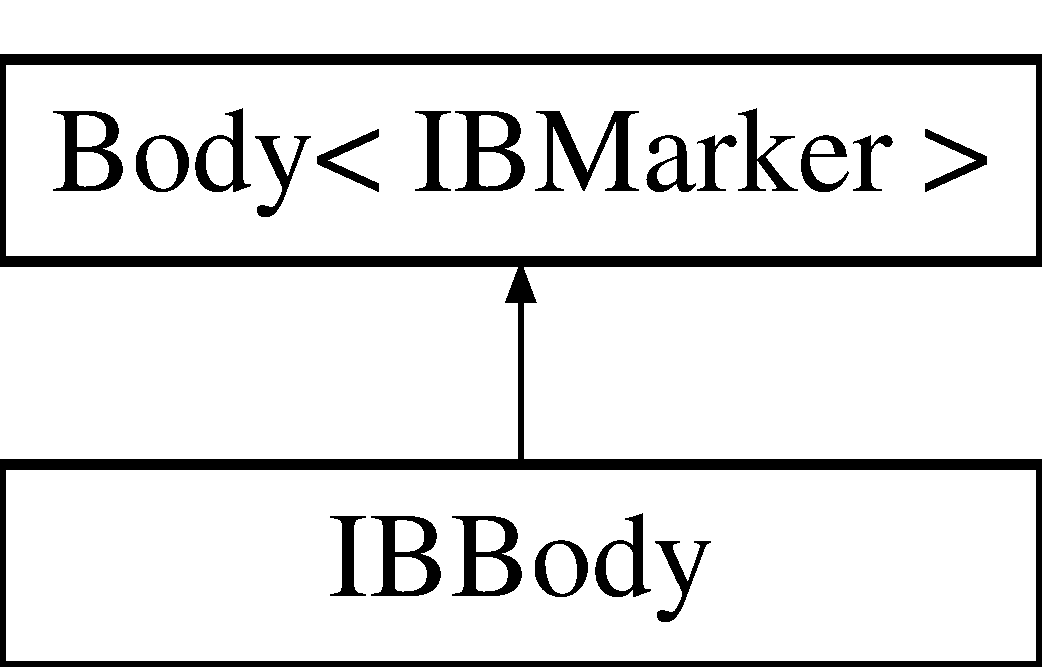
\includegraphics[height=2.000000cm]{class_i_b_body}
\end{center}
\end{figure}
\subsection*{Public Member Functions}
\begin{DoxyCompactItemize}
\item 
\hyperlink{class_i_b_body_a5fbec47db22b9d525724f232d1d81037}{I\+B\+Body} (void)
\begin{DoxyCompactList}\small\item\em Constructor which sets group ID to zero by default. \end{DoxyCompactList}\item 
\hyperlink{class_i_b_body_afe26e702d31e91f562aecd04a5f5c7f0}{$\sim$\+I\+B\+Body} (void)
\begin{DoxyCompactList}\small\item\em Default destructor. \end{DoxyCompactList}\item 
\hyperlink{class_i_b_body_a6ed4dfc0a45739239193b51f415ac5db}{I\+B\+Body} (\hyperlink{class_grid_obj}{Grid\+Obj} $\ast$g)
\begin{DoxyCompactList}\small\item\em Constructor which assigns the owner grid. \end{DoxyCompactList}\item 
void \hyperlink{class_i_b_body_aafa9573e6787bf3b6f07fd3880452b89}{add\+Marker} (double x, double y, double z, bool \hyperlink{class_i_b_body_a526f3e83b45b991a79941ee745698ea5}{flex\+\_\+rigid})
\begin{DoxyCompactList}\small\item\em Method to add an IB marker to the body. \end{DoxyCompactList}\item 
void \hyperlink{class_i_b_body_af26b0107e612dab7cd1e73bac1f4f234}{make\+Body} (double radius, std\+::vector$<$ double $>$ centre, bool \hyperlink{class_i_b_body_a526f3e83b45b991a79941ee745698ea5}{flex\+\_\+rigid}, bool moving, int group)
\begin{DoxyCompactList}\small\item\em Method to seed markers for a sphere / circle. \end{DoxyCompactList}\item 
void \hyperlink{class_i_b_body_a5c3f3da65bdaca7bee4ebea5a06b8bdd}{make\+Body} (std\+::vector$<$ double $>$ width\+\_\+length\+\_\+depth, std\+::vector$<$ double $>$ angles, std\+::vector$<$ double $>$ centre, bool \hyperlink{class_i_b_body_a526f3e83b45b991a79941ee745698ea5}{flex\+\_\+rigid}, bool deform, int group)
\begin{DoxyCompactList}\small\item\em Method to seed markers for a cuboid / rectangle. \end{DoxyCompactList}\item 
void \hyperlink{class_i_b_body_ab83346d555202a5cf669c7e309dc856a}{make\+Body} (int numbermarkers, std\+::vector$<$ double $>$ start\+\_\+point, double fil\+\_\+length, std\+::vector$<$ double $>$ angles, std\+::vector$<$ int $>$ \hyperlink{class_i_b_body_ad9fa313d9cb2c2c463740eed5a1faf16}{B\+Cs}, bool \hyperlink{class_i_b_body_a526f3e83b45b991a79941ee745698ea5}{flex\+\_\+rigid}, bool deform, int group)
\begin{DoxyCompactList}\small\item\em Method to seed markers for a flexible filament. \end{DoxyCompactList}\item 
double \hyperlink{class_i_b_body_a34380e523aef0978495d52bc91f3d74b}{make\+Body} (std\+::vector$<$ double $>$ width\+\_\+length, double angle, std\+::vector$<$ double $>$ centre, bool \hyperlink{class_i_b_body_a526f3e83b45b991a79941ee745698ea5}{flex\+\_\+rigid}, bool deform, int group, bool plate)
\begin{DoxyCompactList}\small\item\em Method to seed markers for a 3D plate inclined from the XZ plane. \end{DoxyCompactList}\item 
void \hyperlink{class_i_b_body_aad21167e57221cb4faf5a15ffebc438d}{make\+Body} (\hyperlink{class_p_cpts}{P\+Cpts} $\ast$\+\_\+\+P\+Cpts)
\begin{DoxyCompactList}\small\item\em Method to build a body from a point cloud. \end{DoxyCompactList}\end{DoxyCompactItemize}
\subsection*{Protected Attributes}
\begin{DoxyCompactItemize}
\item 
bool \hyperlink{class_i_b_body_a526f3e83b45b991a79941ee745698ea5}{flex\+\_\+rigid}
\begin{DoxyCompactList}\small\item\em Flag to indicate flexibility\+: false == rigid body; true == flexible filament. \end{DoxyCompactList}\item 
bool \hyperlink{class_i_b_body_aac0ea66a55dcb0cf41deb2b9a82743e5}{deformable}
\begin{DoxyCompactList}\small\item\em Flag to indicate deformable body\+: false == rigid; true == deformable. \end{DoxyCompactList}\item 
int \hyperlink{class_i_b_body_a4674ade74a2b55ce60a656acfebb4a55}{group\+ID}
\begin{DoxyCompactList}\small\item\em ID of I\+Bbody group -- position updates can be driven from a flexible body in a group. \end{DoxyCompactList}\item 
double \hyperlink{class_i_b_body_a18cd092961f02ecde55363a4d342d098}{delta\+\_\+rho}
\begin{DoxyCompactList}\small\item\em Difference in density between fluid and solid in lattice units. \end{DoxyCompactList}\item 
double \hyperlink{class_i_b_body_a4825a8ef9155062ff9d1011479bd4a9e}{flexural\+\_\+rigidity}
\begin{DoxyCompactList}\small\item\em Young\textquotesingle{}s modulus E $\ast$ Second moment of area I. \end{DoxyCompactList}\item 
std\+::vector$<$ double $>$ \hyperlink{class_i_b_body_ab786e24bc2b303eefcf286e0138cb2d1}{tension}
\begin{DoxyCompactList}\small\item\em Tension between the current marker and its neighbour. \end{DoxyCompactList}\item 
std\+::vector$<$ int $>$ \hyperlink{class_i_b_body_ad9fa313d9cb2c2c463740eed5a1faf16}{B\+Cs}
\begin{DoxyCompactList}\small\item\em B\+Cs type flags (flexible bodies) \end{DoxyCompactList}\end{DoxyCompactItemize}
\subsection*{Friends}
\begin{DoxyCompactItemize}
\item 
class \hyperlink{class_i_b_body_a8b86bdcdb7c54a536293d8632363e114}{Object\+Manager}
\end{DoxyCompactItemize}
\subsection*{Additional Inherited Members}


\subsection{Detailed Description}
Immersed boundary body. 

\subsection{Constructor \& Destructor Documentation}
\index{I\+B\+Body@{I\+B\+Body}!I\+B\+Body@{I\+B\+Body}}
\index{I\+B\+Body@{I\+B\+Body}!I\+B\+Body@{I\+B\+Body}}
\subsubsection[{\texorpdfstring{I\+B\+Body(void)}{IBBody(void)}}]{\setlength{\rightskip}{0pt plus 5cm}I\+B\+Body\+::\+I\+B\+Body (
\begin{DoxyParamCaption}
\item[{void}]{}
\end{DoxyParamCaption}
)}\hypertarget{class_i_b_body_a5fbec47db22b9d525724f232d1d81037}{}\label{class_i_b_body_a5fbec47db22b9d525724f232d1d81037}


Constructor which sets group ID to zero by default. 

\index{I\+B\+Body@{I\+B\+Body}!````~I\+B\+Body@{$\sim$\+I\+B\+Body}}
\index{````~I\+B\+Body@{$\sim$\+I\+B\+Body}!I\+B\+Body@{I\+B\+Body}}
\subsubsection[{\texorpdfstring{$\sim$\+I\+B\+Body(void)}{~IBBody(void)}}]{\setlength{\rightskip}{0pt plus 5cm}I\+B\+Body\+::$\sim$\+I\+B\+Body (
\begin{DoxyParamCaption}
\item[{void}]{}
\end{DoxyParamCaption}
)}\hypertarget{class_i_b_body_afe26e702d31e91f562aecd04a5f5c7f0}{}\label{class_i_b_body_afe26e702d31e91f562aecd04a5f5c7f0}


Default destructor. 

\index{I\+B\+Body@{I\+B\+Body}!I\+B\+Body@{I\+B\+Body}}
\index{I\+B\+Body@{I\+B\+Body}!I\+B\+Body@{I\+B\+Body}}
\subsubsection[{\texorpdfstring{I\+B\+Body(\+Grid\+Obj $\ast$g)}{IBBody(GridObj *g)}}]{\setlength{\rightskip}{0pt plus 5cm}I\+B\+Body\+::\+I\+B\+Body (
\begin{DoxyParamCaption}
\item[{{\bf Grid\+Obj} $\ast$}]{g}
\end{DoxyParamCaption}
)}\hypertarget{class_i_b_body_a6ed4dfc0a45739239193b51f415ac5db}{}\label{class_i_b_body_a6ed4dfc0a45739239193b51f415ac5db}


Constructor which assigns the owner grid. 

Also sets the group ID to zero.


\begin{DoxyParams}{Parameters}
{\em g} & pointer to owner grid \\
\hline
\end{DoxyParams}


\subsection{Member Function Documentation}
\index{I\+B\+Body@{I\+B\+Body}!add\+Marker@{add\+Marker}}
\index{add\+Marker@{add\+Marker}!I\+B\+Body@{I\+B\+Body}}
\subsubsection[{\texorpdfstring{add\+Marker(double x, double y, double z, bool flex\+\_\+rigid)}{addMarker(double x, double y, double z, bool flex_rigid)}}]{\setlength{\rightskip}{0pt plus 5cm}void I\+B\+Body\+::add\+Marker (
\begin{DoxyParamCaption}
\item[{double}]{x, }
\item[{double}]{y, }
\item[{double}]{z, }
\item[{bool}]{flex\+\_\+rigid}
\end{DoxyParamCaption}
)}\hypertarget{class_i_b_body_aafa9573e6787bf3b6f07fd3880452b89}{}\label{class_i_b_body_aafa9573e6787bf3b6f07fd3880452b89}


Method to add an IB marker to the body. 

Adds marker at the given position with the given moving/non-\/moving flag.


\begin{DoxyParams}{Parameters}
{\em x} & x-\/position of marker. \\
\hline
{\em y} & y-\/position of marker. \\
\hline
{\em z} & z-\/position of marker. \\
\hline
{\em flex\+\_\+rigid} & flag to indicate whether marker is movable or not. \\
\hline
\end{DoxyParams}
\index{I\+B\+Body@{I\+B\+Body}!make\+Body@{make\+Body}}
\index{make\+Body@{make\+Body}!I\+B\+Body@{I\+B\+Body}}
\subsubsection[{\texorpdfstring{make\+Body(double radius, std\+::vector$<$ double $>$ centre, bool flex\+\_\+rigid, bool moving, int group)}{makeBody(double radius, std::vector< double > centre, bool flex_rigid, bool moving, int group)}}]{\setlength{\rightskip}{0pt plus 5cm}void I\+B\+Body\+::make\+Body (
\begin{DoxyParamCaption}
\item[{double}]{radius, }
\item[{std\+::vector$<$ double $>$}]{centre, }
\item[{bool}]{flex\+\_\+rigid, }
\item[{bool}]{deform, }
\item[{int}]{group}
\end{DoxyParamCaption}
)}\hypertarget{class_i_b_body_af26b0107e612dab7cd1e73bac1f4f234}{}\label{class_i_b_body_af26b0107e612dab7cd1e73bac1f4f234}


Method to seed markers for a sphere / circle. 


\begin{DoxyParams}{Parameters}
{\em radius} & radius of circle/sphere. \\
\hline
{\em centre} & position vector of circle/sphere centre. \\
\hline
{\em flex\+\_\+rigid} & flag to indicate whether body is flexible and requires a structural calculation. \\
\hline
{\em deform} & flag to indicate whether body is movable and requires relocation each time step. \\
\hline
{\em group} & ID indicating which group the body is part of for collective operations. \\
\hline
\end{DoxyParams}
\index{I\+B\+Body@{I\+B\+Body}!make\+Body@{make\+Body}}
\index{make\+Body@{make\+Body}!I\+B\+Body@{I\+B\+Body}}
\subsubsection[{\texorpdfstring{make\+Body(std\+::vector$<$ double $>$ width\+\_\+length\+\_\+depth, std\+::vector$<$ double $>$ angles, std\+::vector$<$ double $>$ centre, bool flex\+\_\+rigid, bool deform, int group)}{makeBody(std::vector< double > width_length_depth, std::vector< double > angles, std::vector< double > centre, bool flex_rigid, bool deform, int group)}}]{\setlength{\rightskip}{0pt plus 5cm}void I\+B\+Body\+::make\+Body (
\begin{DoxyParamCaption}
\item[{std\+::vector$<$ double $>$}]{width\+\_\+length\+\_\+depth, }
\item[{std\+::vector$<$ double $>$}]{angles, }
\item[{std\+::vector$<$ double $>$}]{centre, }
\item[{bool}]{flex\+\_\+rigid, }
\item[{bool}]{deform, }
\item[{int}]{group}
\end{DoxyParamCaption}
)}\hypertarget{class_i_b_body_a5c3f3da65bdaca7bee4ebea5a06b8bdd}{}\label{class_i_b_body_a5c3f3da65bdaca7bee4ebea5a06b8bdd}


Method to seed markers for a cuboid / rectangle. 


\begin{DoxyParams}{Parameters}
{\em width\+\_\+length\+\_\+depth} & principal dimensions of cuboid / rectangle. \\
\hline
{\em angles} & principal orientation of cuboid / rectangle w.\+r.\+t. domain axes. \\
\hline
{\em centre} & position vector of cuboid / rectangle centre. \\
\hline
{\em flex\+\_\+rigid} & flag to indicate whether body is flexible and requires a structural calculation. \\
\hline
{\em deform} & flag to indicate whether body is movable and requires relocation each time step. \\
\hline
{\em group} & ID indicating which group the body is part of for collective operations. \\
\hline
\end{DoxyParams}
\index{I\+B\+Body@{I\+B\+Body}!make\+Body@{make\+Body}}
\index{make\+Body@{make\+Body}!I\+B\+Body@{I\+B\+Body}}
\subsubsection[{\texorpdfstring{make\+Body(int numbermarkers, std\+::vector$<$ double $>$ start\+\_\+point, double fil\+\_\+length, std\+::vector$<$ double $>$ angles, std\+::vector$<$ int $>$ B\+Cs, bool flex\+\_\+rigid, bool deform, int group)}{makeBody(int numbermarkers, std::vector< double > start_point, double fil_length, std::vector< double > angles, std::vector< int > BCs, bool flex_rigid, bool deform, int group)}}]{\setlength{\rightskip}{0pt plus 5cm}void I\+B\+Body\+::make\+Body (
\begin{DoxyParamCaption}
\item[{int}]{nummarkers, }
\item[{std\+::vector$<$ double $>$}]{start\+\_\+point, }
\item[{double}]{fil\+\_\+length, }
\item[{std\+::vector$<$ double $>$}]{angles, }
\item[{std\+::vector$<$ int $>$}]{B\+Cs, }
\item[{bool}]{flex\+\_\+rigid, }
\item[{bool}]{deform, }
\item[{int}]{group}
\end{DoxyParamCaption}
)}\hypertarget{class_i_b_body_ab83346d555202a5cf669c7e309dc856a}{}\label{class_i_b_body_ab83346d555202a5cf669c7e309dc856a}


Method to seed markers for a flexible filament. 


\begin{DoxyParams}{Parameters}
{\em nummarkers} & number of markers to use for filament. \\
\hline
{\em start\+\_\+point} & 3D position vector of the start of the filament. \\
\hline
{\em fil\+\_\+length} & length of filament in physical units. \\
\hline
{\em angles} & two angles representing filament inclination w.\+r.\+t. domain axes (horizontal plane and vertical plane). \\
\hline
{\em B\+Cs} & vector containing start and end boundary condition types (see class definition for valid values). \\
\hline
{\em flex\+\_\+rigid} & flag to indicate whether body is flexible and requires a structural calculation. \\
\hline
{\em deform} & flag to indicate whether body is movable and requires relocation each time step. \\
\hline
{\em group} & ID indicating which group the body is part of for collective operations. \\
\hline
\end{DoxyParams}
\index{I\+B\+Body@{I\+B\+Body}!make\+Body@{make\+Body}}
\index{make\+Body@{make\+Body}!I\+B\+Body@{I\+B\+Body}}
\subsubsection[{\texorpdfstring{make\+Body(std\+::vector$<$ double $>$ width\+\_\+length, double angle, std\+::vector$<$ double $>$ centre, bool flex\+\_\+rigid, bool deform, int group, bool plate)}{makeBody(std::vector< double > width_length, double angle, std::vector< double > centre, bool flex_rigid, bool deform, int group, bool plate)}}]{\setlength{\rightskip}{0pt plus 5cm}double I\+B\+Body\+::make\+Body (
\begin{DoxyParamCaption}
\item[{std\+::vector$<$ double $>$}]{width\+\_\+length, }
\item[{double}]{angle, }
\item[{std\+::vector$<$ double $>$}]{centre, }
\item[{bool}]{flex\+\_\+rigid, }
\item[{bool}]{deform, }
\item[{int}]{group, }
\item[{bool}]{plate}
\end{DoxyParamCaption}
)}\hypertarget{class_i_b_body_a34380e523aef0978495d52bc91f3d74b}{}\label{class_i_b_body_a34380e523aef0978495d52bc91f3d74b}


Method to seed markers for a 3D plate inclined from the XZ plane. 


\begin{DoxyParams}{Parameters}
{\em width\+\_\+length} & 2D vector of principal dimensions of thin plate. \\
\hline
{\em angle} & inclination angle from horizontal. \\
\hline
{\em centre} & position vector of the plate centre. \\
\hline
{\em flex\+\_\+rigid} & flag to indicate whether body is flexible and requires a structural calculation. \\
\hline
{\em deform} & flag to indicate whether body is movable and requires relocation each time step. \\
\hline
{\em group} & ID indicating which group the body is part of for collective operations. \\
\hline
{\em plate} & arbitrary argument to allow overload otherwise would have the same signature as a filament builder. \\
\hline
\end{DoxyParams}
\index{I\+B\+Body@{I\+B\+Body}!make\+Body@{make\+Body}}
\index{make\+Body@{make\+Body}!I\+B\+Body@{I\+B\+Body}}
\subsubsection[{\texorpdfstring{make\+Body(\+P\+Cpts $\ast$\+\_\+\+P\+Cpts)}{makeBody(PCpts *_PCpts)}}]{\setlength{\rightskip}{0pt plus 5cm}void I\+B\+Body\+::make\+Body (
\begin{DoxyParamCaption}
\item[{{\bf P\+Cpts} $\ast$}]{\+\_\+\+P\+Cpts}
\end{DoxyParamCaption}
)}\hypertarget{class_i_b_body_aad21167e57221cb4faf5a15ffebc438d}{}\label{class_i_b_body_aad21167e57221cb4faf5a15ffebc438d}


Method to build a body from a point cloud. 

Flexibility and deformable properties taken from definitions.


\begin{DoxyParams}{Parameters}
{\em \+\_\+\+P\+Cpts} & pointer to pointer cloud data. \\
\hline
\end{DoxyParams}


\subsection{Friends And Related Function Documentation}
\index{I\+B\+Body@{I\+B\+Body}!Object\+Manager@{Object\+Manager}}
\index{Object\+Manager@{Object\+Manager}!I\+B\+Body@{I\+B\+Body}}
\subsubsection[{\texorpdfstring{Object\+Manager}{ObjectManager}}]{\setlength{\rightskip}{0pt plus 5cm}friend class {\bf Object\+Manager}\hspace{0.3cm}{\ttfamily [friend]}}\hypertarget{class_i_b_body_a8b86bdcdb7c54a536293d8632363e114}{}\label{class_i_b_body_a8b86bdcdb7c54a536293d8632363e114}


\subsection{Member Data Documentation}
\index{I\+B\+Body@{I\+B\+Body}!B\+Cs@{B\+Cs}}
\index{B\+Cs@{B\+Cs}!I\+B\+Body@{I\+B\+Body}}
\subsubsection[{\texorpdfstring{B\+Cs}{BCs}}]{\setlength{\rightskip}{0pt plus 5cm}std\+::vector$<$int$>$ I\+B\+Body\+::\+B\+Cs\hspace{0.3cm}{\ttfamily [protected]}}\hypertarget{class_i_b_body_ad9fa313d9cb2c2c463740eed5a1faf16}{}\label{class_i_b_body_ad9fa313d9cb2c2c463740eed5a1faf16}


B\+Cs type flags (flexible bodies) 

\index{I\+B\+Body@{I\+B\+Body}!deformable@{deformable}}
\index{deformable@{deformable}!I\+B\+Body@{I\+B\+Body}}
\subsubsection[{\texorpdfstring{deformable}{deformable}}]{\setlength{\rightskip}{0pt plus 5cm}bool I\+B\+Body\+::deformable\hspace{0.3cm}{\ttfamily [protected]}}\hypertarget{class_i_b_body_aac0ea66a55dcb0cf41deb2b9a82743e5}{}\label{class_i_b_body_aac0ea66a55dcb0cf41deb2b9a82743e5}


Flag to indicate deformable body\+: false == rigid; true == deformable. 

\index{I\+B\+Body@{I\+B\+Body}!delta\+\_\+rho@{delta\+\_\+rho}}
\index{delta\+\_\+rho@{delta\+\_\+rho}!I\+B\+Body@{I\+B\+Body}}
\subsubsection[{\texorpdfstring{delta\+\_\+rho}{delta_rho}}]{\setlength{\rightskip}{0pt plus 5cm}double I\+B\+Body\+::delta\+\_\+rho\hspace{0.3cm}{\ttfamily [protected]}}\hypertarget{class_i_b_body_a18cd092961f02ecde55363a4d342d098}{}\label{class_i_b_body_a18cd092961f02ecde55363a4d342d098}


Difference in density between fluid and solid in lattice units. 

\index{I\+B\+Body@{I\+B\+Body}!flex\+\_\+rigid@{flex\+\_\+rigid}}
\index{flex\+\_\+rigid@{flex\+\_\+rigid}!I\+B\+Body@{I\+B\+Body}}
\subsubsection[{\texorpdfstring{flex\+\_\+rigid}{flex_rigid}}]{\setlength{\rightskip}{0pt plus 5cm}bool I\+B\+Body\+::flex\+\_\+rigid\hspace{0.3cm}{\ttfamily [protected]}}\hypertarget{class_i_b_body_a526f3e83b45b991a79941ee745698ea5}{}\label{class_i_b_body_a526f3e83b45b991a79941ee745698ea5}


Flag to indicate flexibility\+: false == rigid body; true == flexible filament. 

\index{I\+B\+Body@{I\+B\+Body}!flexural\+\_\+rigidity@{flexural\+\_\+rigidity}}
\index{flexural\+\_\+rigidity@{flexural\+\_\+rigidity}!I\+B\+Body@{I\+B\+Body}}
\subsubsection[{\texorpdfstring{flexural\+\_\+rigidity}{flexural_rigidity}}]{\setlength{\rightskip}{0pt plus 5cm}double I\+B\+Body\+::flexural\+\_\+rigidity\hspace{0.3cm}{\ttfamily [protected]}}\hypertarget{class_i_b_body_a4825a8ef9155062ff9d1011479bd4a9e}{}\label{class_i_b_body_a4825a8ef9155062ff9d1011479bd4a9e}


Young\textquotesingle{}s modulus E $\ast$ Second moment of area I. 

\index{I\+B\+Body@{I\+B\+Body}!group\+ID@{group\+ID}}
\index{group\+ID@{group\+ID}!I\+B\+Body@{I\+B\+Body}}
\subsubsection[{\texorpdfstring{group\+ID}{groupID}}]{\setlength{\rightskip}{0pt plus 5cm}int I\+B\+Body\+::group\+ID\hspace{0.3cm}{\ttfamily [protected]}}\hypertarget{class_i_b_body_a4674ade74a2b55ce60a656acfebb4a55}{}\label{class_i_b_body_a4674ade74a2b55ce60a656acfebb4a55}


ID of I\+Bbody group -- position updates can be driven from a flexible body in a group. 

\index{I\+B\+Body@{I\+B\+Body}!tension@{tension}}
\index{tension@{tension}!I\+B\+Body@{I\+B\+Body}}
\subsubsection[{\texorpdfstring{tension}{tension}}]{\setlength{\rightskip}{0pt plus 5cm}std\+::vector$<$double$>$ I\+B\+Body\+::tension\hspace{0.3cm}{\ttfamily [protected]}}\hypertarget{class_i_b_body_ab786e24bc2b303eefcf286e0138cb2d1}{}\label{class_i_b_body_ab786e24bc2b303eefcf286e0138cb2d1}


Tension between the current marker and its neighbour. 



The documentation for this class was generated from the following files\+:\begin{DoxyCompactItemize}
\item 
\hyperlink{_i_b_body_8h}{I\+B\+Body.\+h}\item 
\hyperlink{_i_b_body_8cpp}{I\+B\+Body.\+cpp}\end{DoxyCompactItemize}

\hypertarget{class_i_b_marker}{}\section{I\+B\+Marker Class Reference}
\label{class_i_b_marker}\index{I\+B\+Marker@{I\+B\+Marker}}


Immersed boundary marker.  




{\ttfamily \#include $<$I\+B\+Marker.\+h$>$}

Inheritance diagram for I\+B\+Marker\+:\begin{figure}[H]
\begin{center}
\leavevmode
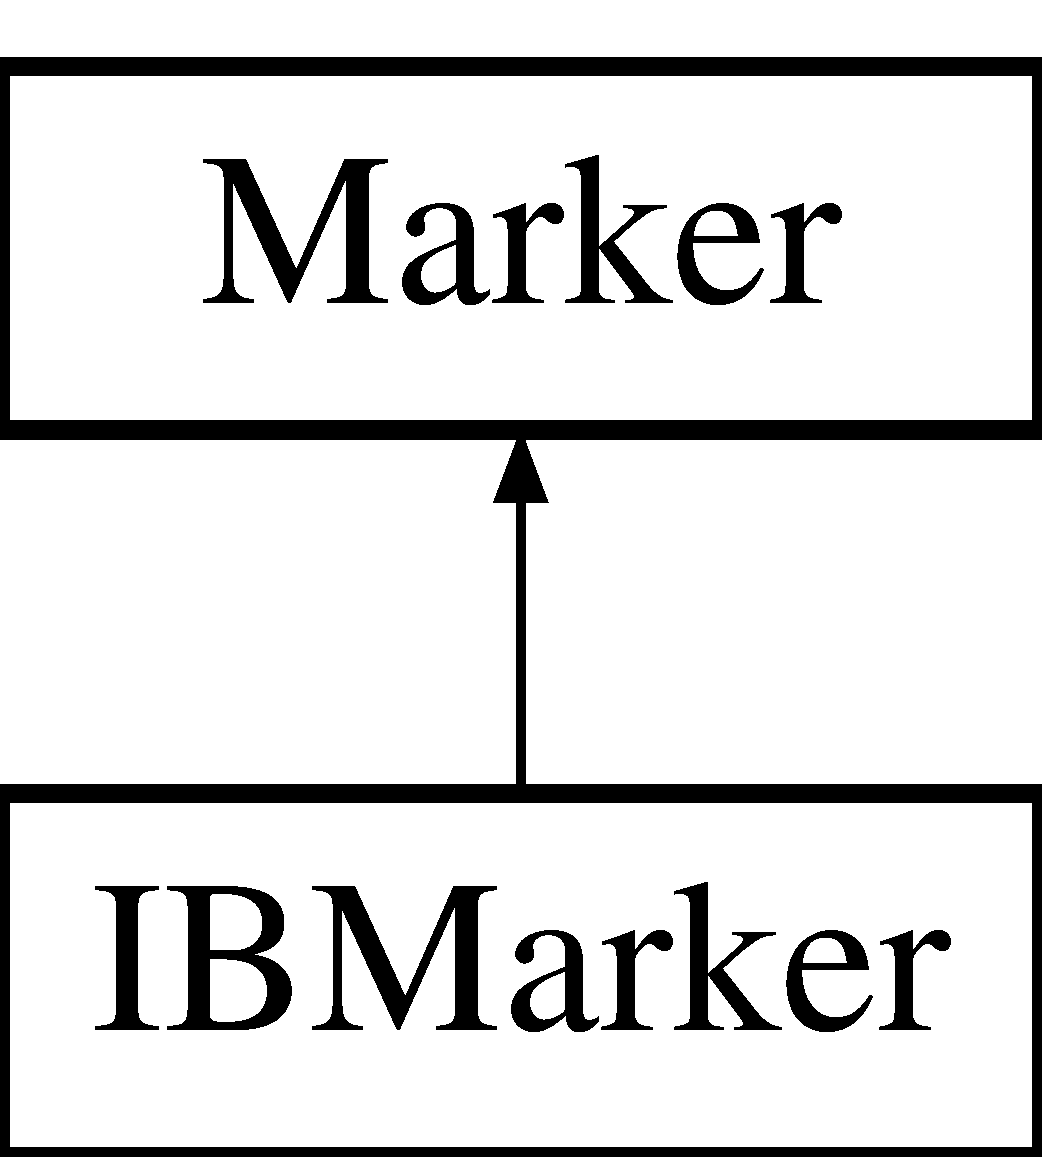
\includegraphics[height=2.000000cm]{class_i_b_marker}
\end{center}
\end{figure}
\subsection*{Public Member Functions}
\begin{DoxyCompactItemize}
\item 
\hyperlink{class_i_b_marker_ab45e9679ae96b75ab7655e738807bb41}{I\+B\+Marker} (void)
\begin{DoxyCompactList}\small\item\em Default constructor. \end{DoxyCompactList}\item 
\hyperlink{class_i_b_marker_a0f3e177c42c3d616a2bbf96c0a9c1099}{$\sim$\+I\+B\+Marker} (void)
\begin{DoxyCompactList}\small\item\em Default destructor. \end{DoxyCompactList}\item 
\hyperlink{class_i_b_marker_a85e4b09f83c97e3dacfa2615d5907e62}{I\+B\+Marker} (double x\+Pos, double y\+Pos, double z\+Pos, \hyperlink{class_grid_obj}{Grid\+Obj} const $\ast$const body\+\_\+owner, bool \hyperlink{class_i_b_marker_a190d90424dc97a7d83669f81dd8273a8}{is\+Flexible}=false)
\begin{DoxyCompactList}\small\item\em Custom constructor with position. \end{DoxyCompactList}\end{DoxyCompactItemize}
\subsection*{Protected Attributes}
\begin{DoxyCompactItemize}
\item 
std\+::vector$<$ double $>$ \hyperlink{class_i_b_marker_aa31ccf45de61bfccc60876ac9e98909a}{fluid\+\_\+vel}
\begin{DoxyCompactList}\small\item\em Fluid velocity interpolated from lattice nodes. \end{DoxyCompactList}\item 
std\+::vector$<$ double $>$ \hyperlink{class_i_b_marker_ad9535b494684533ace9a9523c4df26bf}{desired\+\_\+vel}
\begin{DoxyCompactList}\small\item\em Desired velocity at marker. \end{DoxyCompactList}\item 
std\+::vector$<$ double $>$ \hyperlink{class_i_b_marker_aa8b8b23e64a8bfc4051b95ebf9ccb767}{force\+\_\+xyz}
\begin{DoxyCompactList}\small\item\em Restorative force vector on marker. \end{DoxyCompactList}\item 
std\+::vector$<$ double $>$ \hyperlink{class_i_b_marker_a6a55fe2293f288ae339036ea4a3bc7df}{position\+\_\+old}
\begin{DoxyCompactList}\small\item\em Vector containing the physical coordinates (x,y,z) of the marker at t-\/1. Used for moving bodies. \end{DoxyCompactList}\item 
std\+::vector$<$ double $>$ \hyperlink{class_i_b_marker_a82296e15048c55bd121245d85b076168}{deltaval}
\begin{DoxyCompactList}\small\item\em Value of delta function for a given support node. \end{DoxyCompactList}\item 
bool \hyperlink{class_i_b_marker_a190d90424dc97a7d83669f81dd8273a8}{is\+Flexible}
\begin{DoxyCompactList}\small\item\em Indication as to whether marker is part of a structural or moving body calculation. \end{DoxyCompactList}\item 
double \hyperlink{class_i_b_marker_a8127c61f723299ba0bf04439c1fb1c1e}{epsilon}
\begin{DoxyCompactList}\small\item\em Scaling parameter. \end{DoxyCompactList}\item 
double \hyperlink{class_i_b_marker_aa332dcba1676eae4fbb6d0fa6caca809}{local\+\_\+area}
\begin{DoxyCompactList}\small\item\em Area associated with support node in lattice units (same for all points if from same grid and regularly spaced like L\+BM) \end{DoxyCompactList}\item 
double \hyperlink{class_i_b_marker_a5c908a7e52fc0b2dccbaa277f37b7c22}{dilation}
\begin{DoxyCompactList}\small\item\em Dilation parameter in lattice units (same in all directions for uniform Eulerian grid) \end{DoxyCompactList}\end{DoxyCompactItemize}
\subsection*{Friends}
\begin{DoxyCompactItemize}
\item 
class \hyperlink{class_i_b_marker_a8b86bdcdb7c54a536293d8632363e114}{Object\+Manager}
\item 
class \hyperlink{class_i_b_marker_a5d93aa5aec680a2b395a71266fe4ac92}{I\+B\+Body}
\item 
class \hyperlink{class_i_b_marker_a54980b051e93ff6b0f02df2ff7fee3a8}{I\+B\+Info}
\end{DoxyCompactItemize}
\subsection*{Additional Inherited Members}


\subsection{Detailed Description}
Immersed boundary marker. 

This class declaration is for an immersed boundary Lagrange point. A collection of these points form an immersed boundary body. 

\subsection{Constructor \& Destructor Documentation}
\index{I\+B\+Marker@{I\+B\+Marker}!I\+B\+Marker@{I\+B\+Marker}}
\index{I\+B\+Marker@{I\+B\+Marker}!I\+B\+Marker@{I\+B\+Marker}}
\subsubsection[{\texorpdfstring{I\+B\+Marker(void)}{IBMarker(void)}}]{\setlength{\rightskip}{0pt plus 5cm}I\+B\+Marker\+::\+I\+B\+Marker (
\begin{DoxyParamCaption}
\item[{void}]{}
\end{DoxyParamCaption}
)\hspace{0.3cm}{\ttfamily [inline]}}\hypertarget{class_i_b_marker_ab45e9679ae96b75ab7655e738807bb41}{}\label{class_i_b_marker_ab45e9679ae96b75ab7655e738807bb41}


Default constructor. 

\index{I\+B\+Marker@{I\+B\+Marker}!````~I\+B\+Marker@{$\sim$\+I\+B\+Marker}}
\index{````~I\+B\+Marker@{$\sim$\+I\+B\+Marker}!I\+B\+Marker@{I\+B\+Marker}}
\subsubsection[{\texorpdfstring{$\sim$\+I\+B\+Marker(void)}{~IBMarker(void)}}]{\setlength{\rightskip}{0pt plus 5cm}I\+B\+Marker\+::$\sim$\+I\+B\+Marker (
\begin{DoxyParamCaption}
\item[{void}]{}
\end{DoxyParamCaption}
)\hspace{0.3cm}{\ttfamily [inline]}}\hypertarget{class_i_b_marker_a0f3e177c42c3d616a2bbf96c0a9c1099}{}\label{class_i_b_marker_a0f3e177c42c3d616a2bbf96c0a9c1099}


Default destructor. 

\index{I\+B\+Marker@{I\+B\+Marker}!I\+B\+Marker@{I\+B\+Marker}}
\index{I\+B\+Marker@{I\+B\+Marker}!I\+B\+Marker@{I\+B\+Marker}}
\subsubsection[{\texorpdfstring{I\+B\+Marker(double x\+Pos, double y\+Pos, double z\+Pos, Grid\+Obj const $\ast$const body\+\_\+owner, bool is\+Flexible=false)}{IBMarker(double xPos, double yPos, double zPos, GridObj const *const body_owner, bool isFlexible=false)}}]{\setlength{\rightskip}{0pt plus 5cm}I\+B\+Marker\+::\+I\+B\+Marker (
\begin{DoxyParamCaption}
\item[{double}]{x\+Pos, }
\item[{double}]{y\+Pos, }
\item[{double}]{z\+Pos, }
\item[{{\bf Grid\+Obj} const $\ast$const}]{body\+\_\+owner, }
\item[{bool}]{is\+Flexible = {\ttfamily false}}
\end{DoxyParamCaption}
)}\hypertarget{class_i_b_marker_a85e4b09f83c97e3dacfa2615d5907e62}{}\label{class_i_b_marker_a85e4b09f83c97e3dacfa2615d5907e62}


Custom constructor with position. 


\begin{DoxyParams}{Parameters}
{\em x\+Pos} & x-\/position of marker. \\
\hline
{\em y\+Pos} & y-\/position of marker. \\
\hline
{\em z\+Pos} & z-\/position of marker. \\
\hline
{\em body\+\_\+owner} & Grid on which primary support point is to be found \\
\hline
{\em is\+Flexible} & flag to indicate whether marker is movable or not. \\
\hline
\end{DoxyParams}


\subsection{Friends And Related Function Documentation}
\index{I\+B\+Marker@{I\+B\+Marker}!I\+B\+Body@{I\+B\+Body}}
\index{I\+B\+Body@{I\+B\+Body}!I\+B\+Marker@{I\+B\+Marker}}
\subsubsection[{\texorpdfstring{I\+B\+Body}{IBBody}}]{\setlength{\rightskip}{0pt plus 5cm}friend class {\bf I\+B\+Body}\hspace{0.3cm}{\ttfamily [friend]}}\hypertarget{class_i_b_marker_a5d93aa5aec680a2b395a71266fe4ac92}{}\label{class_i_b_marker_a5d93aa5aec680a2b395a71266fe4ac92}
\index{I\+B\+Marker@{I\+B\+Marker}!I\+B\+Info@{I\+B\+Info}}
\index{I\+B\+Info@{I\+B\+Info}!I\+B\+Marker@{I\+B\+Marker}}
\subsubsection[{\texorpdfstring{I\+B\+Info}{IBInfo}}]{\setlength{\rightskip}{0pt plus 5cm}friend class {\bf I\+B\+Info}\hspace{0.3cm}{\ttfamily [friend]}}\hypertarget{class_i_b_marker_a54980b051e93ff6b0f02df2ff7fee3a8}{}\label{class_i_b_marker_a54980b051e93ff6b0f02df2ff7fee3a8}
\index{I\+B\+Marker@{I\+B\+Marker}!Object\+Manager@{Object\+Manager}}
\index{Object\+Manager@{Object\+Manager}!I\+B\+Marker@{I\+B\+Marker}}
\subsubsection[{\texorpdfstring{Object\+Manager}{ObjectManager}}]{\setlength{\rightskip}{0pt plus 5cm}friend class {\bf Object\+Manager}\hspace{0.3cm}{\ttfamily [friend]}}\hypertarget{class_i_b_marker_a8b86bdcdb7c54a536293d8632363e114}{}\label{class_i_b_marker_a8b86bdcdb7c54a536293d8632363e114}


\subsection{Member Data Documentation}
\index{I\+B\+Marker@{I\+B\+Marker}!deltaval@{deltaval}}
\index{deltaval@{deltaval}!I\+B\+Marker@{I\+B\+Marker}}
\subsubsection[{\texorpdfstring{deltaval}{deltaval}}]{\setlength{\rightskip}{0pt plus 5cm}std\+::vector$<$double$>$ I\+B\+Marker\+::deltaval\hspace{0.3cm}{\ttfamily [protected]}}\hypertarget{class_i_b_marker_a82296e15048c55bd121245d85b076168}{}\label{class_i_b_marker_a82296e15048c55bd121245d85b076168}


Value of delta function for a given support node. 

\index{I\+B\+Marker@{I\+B\+Marker}!desired\+\_\+vel@{desired\+\_\+vel}}
\index{desired\+\_\+vel@{desired\+\_\+vel}!I\+B\+Marker@{I\+B\+Marker}}
\subsubsection[{\texorpdfstring{desired\+\_\+vel}{desired_vel}}]{\setlength{\rightskip}{0pt plus 5cm}std\+::vector$<$double$>$ I\+B\+Marker\+::desired\+\_\+vel\hspace{0.3cm}{\ttfamily [protected]}}\hypertarget{class_i_b_marker_ad9535b494684533ace9a9523c4df26bf}{}\label{class_i_b_marker_ad9535b494684533ace9a9523c4df26bf}


Desired velocity at marker. 

\index{I\+B\+Marker@{I\+B\+Marker}!dilation@{dilation}}
\index{dilation@{dilation}!I\+B\+Marker@{I\+B\+Marker}}
\subsubsection[{\texorpdfstring{dilation}{dilation}}]{\setlength{\rightskip}{0pt plus 5cm}double I\+B\+Marker\+::dilation\hspace{0.3cm}{\ttfamily [protected]}}\hypertarget{class_i_b_marker_a5c908a7e52fc0b2dccbaa277f37b7c22}{}\label{class_i_b_marker_a5c908a7e52fc0b2dccbaa277f37b7c22}


Dilation parameter in lattice units (same in all directions for uniform Eulerian grid) 

\index{I\+B\+Marker@{I\+B\+Marker}!epsilon@{epsilon}}
\index{epsilon@{epsilon}!I\+B\+Marker@{I\+B\+Marker}}
\subsubsection[{\texorpdfstring{epsilon}{epsilon}}]{\setlength{\rightskip}{0pt plus 5cm}double I\+B\+Marker\+::epsilon\hspace{0.3cm}{\ttfamily [protected]}}\hypertarget{class_i_b_marker_a8127c61f723299ba0bf04439c1fb1c1e}{}\label{class_i_b_marker_a8127c61f723299ba0bf04439c1fb1c1e}


Scaling parameter. 

\index{I\+B\+Marker@{I\+B\+Marker}!fluid\+\_\+vel@{fluid\+\_\+vel}}
\index{fluid\+\_\+vel@{fluid\+\_\+vel}!I\+B\+Marker@{I\+B\+Marker}}
\subsubsection[{\texorpdfstring{fluid\+\_\+vel}{fluid_vel}}]{\setlength{\rightskip}{0pt plus 5cm}std\+::vector$<$double$>$ I\+B\+Marker\+::fluid\+\_\+vel\hspace{0.3cm}{\ttfamily [protected]}}\hypertarget{class_i_b_marker_aa31ccf45de61bfccc60876ac9e98909a}{}\label{class_i_b_marker_aa31ccf45de61bfccc60876ac9e98909a}


Fluid velocity interpolated from lattice nodes. 

\index{I\+B\+Marker@{I\+B\+Marker}!force\+\_\+xyz@{force\+\_\+xyz}}
\index{force\+\_\+xyz@{force\+\_\+xyz}!I\+B\+Marker@{I\+B\+Marker}}
\subsubsection[{\texorpdfstring{force\+\_\+xyz}{force_xyz}}]{\setlength{\rightskip}{0pt plus 5cm}std\+::vector$<$double$>$ I\+B\+Marker\+::force\+\_\+xyz\hspace{0.3cm}{\ttfamily [protected]}}\hypertarget{class_i_b_marker_aa8b8b23e64a8bfc4051b95ebf9ccb767}{}\label{class_i_b_marker_aa8b8b23e64a8bfc4051b95ebf9ccb767}


Restorative force vector on marker. 

\index{I\+B\+Marker@{I\+B\+Marker}!is\+Flexible@{is\+Flexible}}
\index{is\+Flexible@{is\+Flexible}!I\+B\+Marker@{I\+B\+Marker}}
\subsubsection[{\texorpdfstring{is\+Flexible}{isFlexible}}]{\setlength{\rightskip}{0pt plus 5cm}bool I\+B\+Marker\+::is\+Flexible\hspace{0.3cm}{\ttfamily [protected]}}\hypertarget{class_i_b_marker_a190d90424dc97a7d83669f81dd8273a8}{}\label{class_i_b_marker_a190d90424dc97a7d83669f81dd8273a8}


Indication as to whether marker is part of a structural or moving body calculation. 

\index{I\+B\+Marker@{I\+B\+Marker}!local\+\_\+area@{local\+\_\+area}}
\index{local\+\_\+area@{local\+\_\+area}!I\+B\+Marker@{I\+B\+Marker}}
\subsubsection[{\texorpdfstring{local\+\_\+area}{local_area}}]{\setlength{\rightskip}{0pt plus 5cm}double I\+B\+Marker\+::local\+\_\+area\hspace{0.3cm}{\ttfamily [protected]}}\hypertarget{class_i_b_marker_aa332dcba1676eae4fbb6d0fa6caca809}{}\label{class_i_b_marker_aa332dcba1676eae4fbb6d0fa6caca809}


Area associated with support node in lattice units (same for all points if from same grid and regularly spaced like L\+BM) 

\index{I\+B\+Marker@{I\+B\+Marker}!position\+\_\+old@{position\+\_\+old}}
\index{position\+\_\+old@{position\+\_\+old}!I\+B\+Marker@{I\+B\+Marker}}
\subsubsection[{\texorpdfstring{position\+\_\+old}{position_old}}]{\setlength{\rightskip}{0pt plus 5cm}std\+::vector$<$double$>$ I\+B\+Marker\+::position\+\_\+old\hspace{0.3cm}{\ttfamily [protected]}}\hypertarget{class_i_b_marker_a6a55fe2293f288ae339036ea4a3bc7df}{}\label{class_i_b_marker_a6a55fe2293f288ae339036ea4a3bc7df}


Vector containing the physical coordinates (x,y,z) of the marker at t-\/1. Used for moving bodies. 



The documentation for this class was generated from the following files\+:\begin{DoxyCompactItemize}
\item 
\hyperlink{_i_b_marker_8h}{I\+B\+Marker.\+h}\item 
\hyperlink{_i_b_marker_8cpp}{I\+B\+Marker.\+cpp}\end{DoxyCompactItemize}

\hypertarget{class_i_vector}{}\section{I\+Vector$<$ Gen\+Typ $>$ Class Template Reference}
\label{class_i_vector}\index{I\+Vector$<$ Gen\+Typ $>$@{I\+Vector$<$ Gen\+Typ $>$}}


{\ttfamily \#include $<$I\+Vector.\+h$>$}

Inheritance diagram for I\+Vector$<$ Gen\+Typ $>$\+:\begin{figure}[H]
\begin{center}
\leavevmode
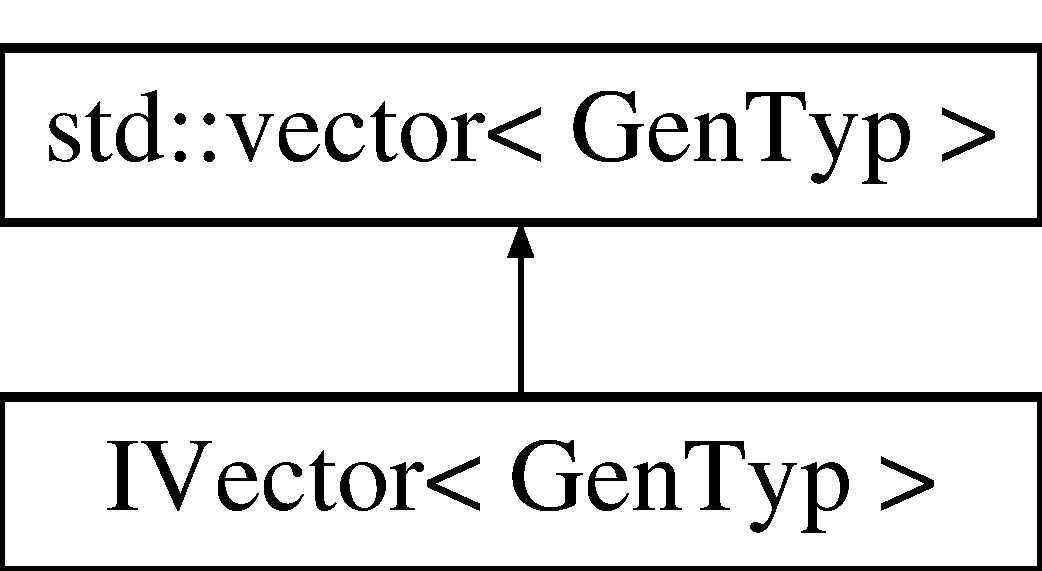
\includegraphics[height=2.000000cm]{class_i_vector}
\end{center}
\end{figure}
\subsection*{Public Member Functions}
\begin{DoxyCompactItemize}
\item 
\hyperlink{class_i_vector_aa9e08edf18a107b1512c563f974b84a9}{I\+Vector} ()
\item 
\hyperlink{class_i_vector_a98498962689499607ff2f3c0dd251c55}{$\sim$\+I\+Vector} ()
\item 
\hyperlink{class_i_vector_aa20ed511fdb06743b435f23bbf286e8c}{I\+Vector} (size\+\_\+t size, Gen\+Typ val)
\item 
Gen\+Typ \& \hyperlink{class_i_vector_aecbb48fdf561c44efb89127c77ab11e2}{operator()} (size\+\_\+t i, size\+\_\+t j, size\+\_\+t k, size\+\_\+t v, size\+\_\+t j\+\_\+max, size\+\_\+t k\+\_\+max, size\+\_\+t v\+\_\+max)
\item 
Gen\+Typ \& \hyperlink{class_i_vector_a975461485fb45bd7e970822800266177}{operator()} (size\+\_\+t i, size\+\_\+t j, size\+\_\+t k, size\+\_\+t j\+\_\+max, size\+\_\+t k\+\_\+max)
\item 
Gen\+Typ \& \hyperlink{class_i_vector_a506334a0add9a0a79e27a208fda53c0d}{operator()} (size\+\_\+t i, size\+\_\+t j, size\+\_\+t j\+\_\+max)
\end{DoxyCompactItemize}


\subsection{Constructor \& Destructor Documentation}
\index{I\+Vector@{I\+Vector}!I\+Vector@{I\+Vector}}
\index{I\+Vector@{I\+Vector}!I\+Vector@{I\+Vector}}
\subsubsection[{\texorpdfstring{I\+Vector()}{IVector()}}]{\setlength{\rightskip}{0pt plus 5cm}template$<$typename Gen\+Typ$>$ {\bf I\+Vector}$<$ Gen\+Typ $>$\+::{\bf I\+Vector} (
\begin{DoxyParamCaption}
{}
\end{DoxyParamCaption}
)\hspace{0.3cm}{\ttfamily [inline]}}\hypertarget{class_i_vector_aa9e08edf18a107b1512c563f974b84a9}{}\label{class_i_vector_aa9e08edf18a107b1512c563f974b84a9}
\index{I\+Vector@{I\+Vector}!````~I\+Vector@{$\sim$\+I\+Vector}}
\index{````~I\+Vector@{$\sim$\+I\+Vector}!I\+Vector@{I\+Vector}}
\subsubsection[{\texorpdfstring{$\sim$\+I\+Vector()}{~IVector()}}]{\setlength{\rightskip}{0pt plus 5cm}template$<$typename Gen\+Typ$>$ {\bf I\+Vector}$<$ Gen\+Typ $>$\+::$\sim${\bf I\+Vector} (
\begin{DoxyParamCaption}
{}
\end{DoxyParamCaption}
)\hspace{0.3cm}{\ttfamily [inline]}}\hypertarget{class_i_vector_a98498962689499607ff2f3c0dd251c55}{}\label{class_i_vector_a98498962689499607ff2f3c0dd251c55}
\index{I\+Vector@{I\+Vector}!I\+Vector@{I\+Vector}}
\index{I\+Vector@{I\+Vector}!I\+Vector@{I\+Vector}}
\subsubsection[{\texorpdfstring{I\+Vector(size\+\_\+t size, Gen\+Typ val)}{IVector(size_t size, GenTyp val)}}]{\setlength{\rightskip}{0pt plus 5cm}template$<$typename Gen\+Typ$>$ {\bf I\+Vector}$<$ Gen\+Typ $>$\+::{\bf I\+Vector} (
\begin{DoxyParamCaption}
\item[{size\+\_\+t}]{size, }
\item[{Gen\+Typ}]{val}
\end{DoxyParamCaption}
)\hspace{0.3cm}{\ttfamily [inline]}}\hypertarget{class_i_vector_aa20ed511fdb06743b435f23bbf286e8c}{}\label{class_i_vector_aa20ed511fdb06743b435f23bbf286e8c}


\subsection{Member Function Documentation}
\index{I\+Vector@{I\+Vector}!operator()@{operator()}}
\index{operator()@{operator()}!I\+Vector@{I\+Vector}}
\subsubsection[{\texorpdfstring{operator()(size\+\_\+t i, size\+\_\+t j, size\+\_\+t k, size\+\_\+t v, size\+\_\+t j\+\_\+max, size\+\_\+t k\+\_\+max, size\+\_\+t v\+\_\+max)}{operator()(size_t i, size_t j, size_t k, size_t v, size_t j_max, size_t k_max, size_t v_max)}}]{\setlength{\rightskip}{0pt plus 5cm}template$<$typename Gen\+Typ$>$ Gen\+Typ\& {\bf I\+Vector}$<$ Gen\+Typ $>$\+::operator() (
\begin{DoxyParamCaption}
\item[{size\+\_\+t}]{i, }
\item[{size\+\_\+t}]{j, }
\item[{size\+\_\+t}]{k, }
\item[{size\+\_\+t}]{v, }
\item[{size\+\_\+t}]{j\+\_\+max, }
\item[{size\+\_\+t}]{k\+\_\+max, }
\item[{size\+\_\+t}]{v\+\_\+max}
\end{DoxyParamCaption}
)\hspace{0.3cm}{\ttfamily [inline]}}\hypertarget{class_i_vector_aecbb48fdf561c44efb89127c77ab11e2}{}\label{class_i_vector_aecbb48fdf561c44efb89127c77ab11e2}
\index{I\+Vector@{I\+Vector}!operator()@{operator()}}
\index{operator()@{operator()}!I\+Vector@{I\+Vector}}
\subsubsection[{\texorpdfstring{operator()(size\+\_\+t i, size\+\_\+t j, size\+\_\+t k, size\+\_\+t j\+\_\+max, size\+\_\+t k\+\_\+max)}{operator()(size_t i, size_t j, size_t k, size_t j_max, size_t k_max)}}]{\setlength{\rightskip}{0pt plus 5cm}template$<$typename Gen\+Typ$>$ Gen\+Typ\& {\bf I\+Vector}$<$ Gen\+Typ $>$\+::operator() (
\begin{DoxyParamCaption}
\item[{size\+\_\+t}]{i, }
\item[{size\+\_\+t}]{j, }
\item[{size\+\_\+t}]{k, }
\item[{size\+\_\+t}]{j\+\_\+max, }
\item[{size\+\_\+t}]{k\+\_\+max}
\end{DoxyParamCaption}
)\hspace{0.3cm}{\ttfamily [inline]}}\hypertarget{class_i_vector_a975461485fb45bd7e970822800266177}{}\label{class_i_vector_a975461485fb45bd7e970822800266177}
\index{I\+Vector@{I\+Vector}!operator()@{operator()}}
\index{operator()@{operator()}!I\+Vector@{I\+Vector}}
\subsubsection[{\texorpdfstring{operator()(size\+\_\+t i, size\+\_\+t j, size\+\_\+t j\+\_\+max)}{operator()(size_t i, size_t j, size_t j_max)}}]{\setlength{\rightskip}{0pt plus 5cm}template$<$typename Gen\+Typ$>$ Gen\+Typ\& {\bf I\+Vector}$<$ Gen\+Typ $>$\+::operator() (
\begin{DoxyParamCaption}
\item[{size\+\_\+t}]{i, }
\item[{size\+\_\+t}]{j, }
\item[{size\+\_\+t}]{j\+\_\+max}
\end{DoxyParamCaption}
)\hspace{0.3cm}{\ttfamily [inline]}}\hypertarget{class_i_vector_a506334a0add9a0a79e27a208fda53c0d}{}\label{class_i_vector_a506334a0add9a0a79e27a208fda53c0d}


The documentation for this class was generated from the following file\+:\begin{DoxyCompactItemize}
\item 
\hyperlink{_i_vector_8h}{I\+Vector.\+h}\end{DoxyCompactItemize}

\hypertarget{struct_mpi_manager_1_1layer__edges}{}\section{Mpi\+Manager\+:\+:layer\+\_\+edges Struct Reference}
\label{struct_mpi_manager_1_1layer__edges}\index{Mpi\+Manager\+::layer\+\_\+edges@{Mpi\+Manager\+::layer\+\_\+edges}}


Structure containing absolute positions of the edges of halos.  




{\ttfamily \#include $<$Mpi\+Manager.\+h$>$}

\subsection*{Public Attributes}
\begin{DoxyCompactItemize}
\item 
double \hyperlink{struct_mpi_manager_1_1layer__edges_a9f79fa4b504f2d4418f2bc4747cc908c}{X} \mbox{[}4\mbox{]}
\begin{DoxyCompactList}\small\item\em X limits. \end{DoxyCompactList}\item 
double \hyperlink{struct_mpi_manager_1_1layer__edges_aa4d880e027a6410ff4b34e28dcd1f9d4}{Y} \mbox{[}4\mbox{]}
\begin{DoxyCompactList}\small\item\em Y limits. \end{DoxyCompactList}\item 
double \hyperlink{struct_mpi_manager_1_1layer__edges_a25eea1176a0c06c1e25a7a08b8840283}{Z} \mbox{[}4\mbox{]}
\begin{DoxyCompactList}\small\item\em Z limits. \end{DoxyCompactList}\end{DoxyCompactItemize}


\subsection{Detailed Description}
Structure containing absolute positions of the edges of halos. 

Sender (inner) and receiver (outer) parts of halo are located using the convention \mbox{[}left\+\_\+min left\+\_\+max right\+\_\+min right\+\_\+max\mbox{]} for X and similar for Y and Z. Access using the enumerator e\+Edge\+Min\+Max. 

\subsection{Member Data Documentation}
\index{Mpi\+Manager\+::layer\+\_\+edges@{Mpi\+Manager\+::layer\+\_\+edges}!X@{X}}
\index{X@{X}!Mpi\+Manager\+::layer\+\_\+edges@{Mpi\+Manager\+::layer\+\_\+edges}}
\subsubsection[{\texorpdfstring{X}{X}}]{\setlength{\rightskip}{0pt plus 5cm}double Mpi\+Manager\+::layer\+\_\+edges\+::X\mbox{[}4\mbox{]}}\hypertarget{struct_mpi_manager_1_1layer__edges_a9f79fa4b504f2d4418f2bc4747cc908c}{}\label{struct_mpi_manager_1_1layer__edges_a9f79fa4b504f2d4418f2bc4747cc908c}


X limits. 

\index{Mpi\+Manager\+::layer\+\_\+edges@{Mpi\+Manager\+::layer\+\_\+edges}!Y@{Y}}
\index{Y@{Y}!Mpi\+Manager\+::layer\+\_\+edges@{Mpi\+Manager\+::layer\+\_\+edges}}
\subsubsection[{\texorpdfstring{Y}{Y}}]{\setlength{\rightskip}{0pt plus 5cm}double Mpi\+Manager\+::layer\+\_\+edges\+::Y\mbox{[}4\mbox{]}}\hypertarget{struct_mpi_manager_1_1layer__edges_aa4d880e027a6410ff4b34e28dcd1f9d4}{}\label{struct_mpi_manager_1_1layer__edges_aa4d880e027a6410ff4b34e28dcd1f9d4}


Y limits. 

\index{Mpi\+Manager\+::layer\+\_\+edges@{Mpi\+Manager\+::layer\+\_\+edges}!Z@{Z}}
\index{Z@{Z}!Mpi\+Manager\+::layer\+\_\+edges@{Mpi\+Manager\+::layer\+\_\+edges}}
\subsubsection[{\texorpdfstring{Z}{Z}}]{\setlength{\rightskip}{0pt plus 5cm}double Mpi\+Manager\+::layer\+\_\+edges\+::Z\mbox{[}4\mbox{]}}\hypertarget{struct_mpi_manager_1_1layer__edges_a25eea1176a0c06c1e25a7a08b8840283}{}\label{struct_mpi_manager_1_1layer__edges_a25eea1176a0c06c1e25a7a08b8840283}


Z limits. 



The documentation for this struct was generated from the following file\+:\begin{DoxyCompactItemize}
\item 
\hyperlink{_mpi_manager_8h}{Mpi\+Manager.\+h}\end{DoxyCompactItemize}

\hypertarget{class_marker}{}\section{Marker Class Reference}
\label{class_marker}\index{Marker@{Marker}}


Generic marker class.  




{\ttfamily \#include $<$Marker.\+h$>$}

Inheritance diagram for Marker\+:\begin{figure}[H]
\begin{center}
\leavevmode
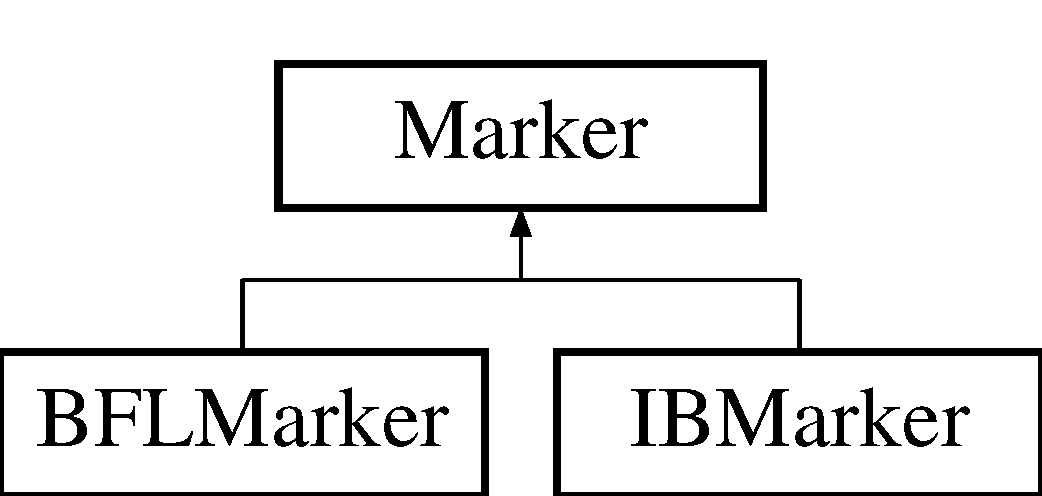
\includegraphics[height=2.000000cm]{class_marker}
\end{center}
\end{figure}
\subsection*{Public Member Functions}
\begin{DoxyCompactItemize}
\item 
\hyperlink{class_marker_ac09c0211aaad490b0dd4ac448c69ba36}{Marker} (void)
\begin{DoxyCompactList}\small\item\em Default constructor. \end{DoxyCompactList}\item 
\hyperlink{class_marker_ac34f00758cfb07bcf550209083633eb6}{$\sim$\+Marker} (void)
\begin{DoxyCompactList}\small\item\em Default destructor. \end{DoxyCompactList}\item 
\hyperlink{class_marker_a39d86412648446a87719fd9a68c4f34b}{Marker} (double x, double y, double z, \hyperlink{class_grid_obj}{Grid\+Obj} const $\ast$const body\+\_\+owner)
\begin{DoxyCompactList}\small\item\em Custom constructor which locates marker. \end{DoxyCompactList}\end{DoxyCompactItemize}
\subsection*{Public Attributes}
\begin{DoxyCompactItemize}
\item 
std\+::vector$<$ double $>$ \hyperlink{class_marker_a988d209a817df43124a100fb54b00b70}{position}
\begin{DoxyCompactList}\small\item\em Position vector of marker location in physical units. \end{DoxyCompactList}\item 
std\+::vector$<$ int $>$ \hyperlink{class_marker_af2b0bab614609f2e9c5bebc1db3f8174}{supp\+\_\+i}
\begin{DoxyCompactList}\small\item\em X-\/indices of lattice sites in support of this marker. \end{DoxyCompactList}\item 
std\+::vector$<$ int $>$ \hyperlink{class_marker_a400ae7b896edf2abe0403dde435b0977}{supp\+\_\+j}
\begin{DoxyCompactList}\small\item\em Y-\/indices of lattice sites in support of this marker. \end{DoxyCompactList}\item 
std\+::vector$<$ int $>$ \hyperlink{class_marker_ab06b6d2cfb7221579cf32538f0c79b82}{supp\+\_\+k}
\begin{DoxyCompactList}\small\item\em Z-\/indices of lattice sites in support of this marker. \end{DoxyCompactList}\item 
std\+::vector$<$ int $>$ \hyperlink{class_marker_a183752ab41e56b159570a103c25f2aec}{support\+\_\+rank}
\begin{DoxyCompactList}\small\item\em Array of indices indicating on which rank the given support point resides. \end{DoxyCompactList}\end{DoxyCompactItemize}


\subsection{Detailed Description}
Generic marker class. 

\subsection{Constructor \& Destructor Documentation}
\index{Marker@{Marker}!Marker@{Marker}}
\index{Marker@{Marker}!Marker@{Marker}}
\subsubsection[{\texorpdfstring{Marker(void)}{Marker(void)}}]{\setlength{\rightskip}{0pt plus 5cm}Marker\+::\+Marker (
\begin{DoxyParamCaption}
\item[{void}]{}
\end{DoxyParamCaption}
)\hspace{0.3cm}{\ttfamily [inline]}}\hypertarget{class_marker_ac09c0211aaad490b0dd4ac448c69ba36}{}\label{class_marker_ac09c0211aaad490b0dd4ac448c69ba36}


Default constructor. 

\index{Marker@{Marker}!````~Marker@{$\sim$\+Marker}}
\index{````~Marker@{$\sim$\+Marker}!Marker@{Marker}}
\subsubsection[{\texorpdfstring{$\sim$\+Marker(void)}{~Marker(void)}}]{\setlength{\rightskip}{0pt plus 5cm}Marker\+::$\sim$\+Marker (
\begin{DoxyParamCaption}
\item[{void}]{}
\end{DoxyParamCaption}
)\hspace{0.3cm}{\ttfamily [inline]}}\hypertarget{class_marker_ac34f00758cfb07bcf550209083633eb6}{}\label{class_marker_ac34f00758cfb07bcf550209083633eb6}


Default destructor. 

\index{Marker@{Marker}!Marker@{Marker}}
\index{Marker@{Marker}!Marker@{Marker}}
\subsubsection[{\texorpdfstring{Marker(double x, double y, double z, Grid\+Obj const $\ast$const body\+\_\+owner)}{Marker(double x, double y, double z, GridObj const *const body_owner)}}]{\setlength{\rightskip}{0pt plus 5cm}Marker\+::\+Marker (
\begin{DoxyParamCaption}
\item[{double}]{x, }
\item[{double}]{y, }
\item[{double}]{z, }
\item[{{\bf Grid\+Obj} const $\ast$const}]{body\+\_\+owner}
\end{DoxyParamCaption}
)\hspace{0.3cm}{\ttfamily [inline]}}\hypertarget{class_marker_a39d86412648446a87719fd9a68c4f34b}{}\label{class_marker_a39d86412648446a87719fd9a68c4f34b}


Custom constructor which locates marker. 

In order to properley initialise during construction, a grid should be passed in on which primary support point can be found.


\begin{DoxyParams}{Parameters}
{\em x} & X-\/position of marker \\
\hline
{\em y} & Y-\/position of marker \\
\hline
{\em z} & Z-\/position of marker \\
\hline
{\em body\+\_\+owner} & Grid on which primary support point is to be found. \\
\hline
\end{DoxyParams}


\subsection{Member Data Documentation}
\index{Marker@{Marker}!position@{position}}
\index{position@{position}!Marker@{Marker}}
\subsubsection[{\texorpdfstring{position}{position}}]{\setlength{\rightskip}{0pt plus 5cm}std\+::vector$<$double$>$ Marker\+::position}\hypertarget{class_marker_a988d209a817df43124a100fb54b00b70}{}\label{class_marker_a988d209a817df43124a100fb54b00b70}


Position vector of marker location in physical units. 

\index{Marker@{Marker}!supp\+\_\+i@{supp\+\_\+i}}
\index{supp\+\_\+i@{supp\+\_\+i}!Marker@{Marker}}
\subsubsection[{\texorpdfstring{supp\+\_\+i}{supp_i}}]{\setlength{\rightskip}{0pt plus 5cm}std\+::vector$<$int$>$ Marker\+::supp\+\_\+i}\hypertarget{class_marker_af2b0bab614609f2e9c5bebc1db3f8174}{}\label{class_marker_af2b0bab614609f2e9c5bebc1db3f8174}


X-\/indices of lattice sites in support of this marker. 

\index{Marker@{Marker}!supp\+\_\+j@{supp\+\_\+j}}
\index{supp\+\_\+j@{supp\+\_\+j}!Marker@{Marker}}
\subsubsection[{\texorpdfstring{supp\+\_\+j}{supp_j}}]{\setlength{\rightskip}{0pt plus 5cm}std\+::vector$<$int$>$ Marker\+::supp\+\_\+j}\hypertarget{class_marker_a400ae7b896edf2abe0403dde435b0977}{}\label{class_marker_a400ae7b896edf2abe0403dde435b0977}


Y-\/indices of lattice sites in support of this marker. 

\index{Marker@{Marker}!supp\+\_\+k@{supp\+\_\+k}}
\index{supp\+\_\+k@{supp\+\_\+k}!Marker@{Marker}}
\subsubsection[{\texorpdfstring{supp\+\_\+k}{supp_k}}]{\setlength{\rightskip}{0pt plus 5cm}std\+::vector$<$int$>$ Marker\+::supp\+\_\+k}\hypertarget{class_marker_ab06b6d2cfb7221579cf32538f0c79b82}{}\label{class_marker_ab06b6d2cfb7221579cf32538f0c79b82}


Z-\/indices of lattice sites in support of this marker. 

\index{Marker@{Marker}!support\+\_\+rank@{support\+\_\+rank}}
\index{support\+\_\+rank@{support\+\_\+rank}!Marker@{Marker}}
\subsubsection[{\texorpdfstring{support\+\_\+rank}{support_rank}}]{\setlength{\rightskip}{0pt plus 5cm}std\+::vector$<$int$>$ Marker\+::support\+\_\+rank}\hypertarget{class_marker_a183752ab41e56b159570a103c25f2aec}{}\label{class_marker_a183752ab41e56b159570a103c25f2aec}


Array of indices indicating on which rank the given support point resides. 



The documentation for this class was generated from the following file\+:\begin{DoxyCompactItemize}
\item 
\hyperlink{_marker_8h}{Marker.\+h}\end{DoxyCompactItemize}

\hypertarget{class_marker_data}{}\section{Marker\+Data Class Reference}
\label{class_marker_data}\index{Marker\+Data@{Marker\+Data}}


{\ttfamily \#include $<$Body.\+h$>$}

\subsection*{Public Member Functions}
\begin{DoxyCompactItemize}
\item 
\hyperlink{class_marker_data_a6893b09af012bdf7ab510f8b491ca40e}{Marker\+Data} (int \hyperlink{class_marker_data_abb9f15d2132f7007cf0612d53cd969db}{i}, int \hyperlink{class_marker_data_ae48473a1571656cf8f02403cb42a4adc}{j}, int \hyperlink{class_marker_data_a66183b4e9a166279551f4c180d0d71c8}{k}, double \hyperlink{class_marker_data_aade1e2f618efa75989831f028db027cd}{x}, double \hyperlink{class_marker_data_a9b10ce07e886a94fc10e097b2cef2265}{y}, double \hyperlink{class_marker_data_adc00ff164746747a7b379a94abf8a2df}{z}, int \hyperlink{class_marker_data_aae16e1f3245f8ef95ed6170e3775669d}{ID})
\item 
\hyperlink{class_marker_data_a9314e10d84afacc7c6eb6e1fec9c8cf7}{Marker\+Data} (void)
\item 
\hyperlink{class_marker_data_aa2f67eda451a48ab5cc4162e12b675e0}{$\sim$\+Marker\+Data} (void)
\end{DoxyCompactItemize}
\subsection*{Public Attributes}
\begin{DoxyCompactItemize}
\item 
int \hyperlink{class_marker_data_abb9f15d2132f7007cf0612d53cd969db}{i}
\item 
int \hyperlink{class_marker_data_ae48473a1571656cf8f02403cb42a4adc}{j}
\item 
int \hyperlink{class_marker_data_a66183b4e9a166279551f4c180d0d71c8}{k}
\item 
int \hyperlink{class_marker_data_aae16e1f3245f8ef95ed6170e3775669d}{ID}
\item 
double \hyperlink{class_marker_data_aade1e2f618efa75989831f028db027cd}{x}
\item 
double \hyperlink{class_marker_data_a9b10ce07e886a94fc10e097b2cef2265}{y}
\item 
double \hyperlink{class_marker_data_adc00ff164746747a7b379a94abf8a2df}{z}
\end{DoxyCompactItemize}


\subsection{Constructor \& Destructor Documentation}
\index{Marker\+Data@{Marker\+Data}!Marker\+Data@{Marker\+Data}}
\index{Marker\+Data@{Marker\+Data}!Marker\+Data@{Marker\+Data}}
\subsubsection[{\texorpdfstring{Marker\+Data(int i, int j, int k, double x, double y, double z, int I\+D)}{MarkerData(int i, int j, int k, double x, double y, double z, int ID)}}]{\setlength{\rightskip}{0pt plus 5cm}Marker\+Data\+::\+Marker\+Data (
\begin{DoxyParamCaption}
\item[{int}]{i, }
\item[{int}]{j, }
\item[{int}]{k, }
\item[{double}]{x, }
\item[{double}]{y, }
\item[{double}]{z, }
\item[{int}]{ID}
\end{DoxyParamCaption}
)\hspace{0.3cm}{\ttfamily [inline]}}\hypertarget{class_marker_data_a6893b09af012bdf7ab510f8b491ca40e}{}\label{class_marker_data_a6893b09af012bdf7ab510f8b491ca40e}
\index{Marker\+Data@{Marker\+Data}!Marker\+Data@{Marker\+Data}}
\index{Marker\+Data@{Marker\+Data}!Marker\+Data@{Marker\+Data}}
\subsubsection[{\texorpdfstring{Marker\+Data(void)}{MarkerData(void)}}]{\setlength{\rightskip}{0pt plus 5cm}Marker\+Data\+::\+Marker\+Data (
\begin{DoxyParamCaption}
\item[{void}]{}
\end{DoxyParamCaption}
)\hspace{0.3cm}{\ttfamily [inline]}}\hypertarget{class_marker_data_a9314e10d84afacc7c6eb6e1fec9c8cf7}{}\label{class_marker_data_a9314e10d84afacc7c6eb6e1fec9c8cf7}
\index{Marker\+Data@{Marker\+Data}!````~Marker\+Data@{$\sim$\+Marker\+Data}}
\index{````~Marker\+Data@{$\sim$\+Marker\+Data}!Marker\+Data@{Marker\+Data}}
\subsubsection[{\texorpdfstring{$\sim$\+Marker\+Data(void)}{~MarkerData(void)}}]{\setlength{\rightskip}{0pt plus 5cm}Marker\+Data\+::$\sim$\+Marker\+Data (
\begin{DoxyParamCaption}
\item[{void}]{}
\end{DoxyParamCaption}
)\hspace{0.3cm}{\ttfamily [inline]}}\hypertarget{class_marker_data_aa2f67eda451a48ab5cc4162e12b675e0}{}\label{class_marker_data_aa2f67eda451a48ab5cc4162e12b675e0}


\subsection{Member Data Documentation}
\index{Marker\+Data@{Marker\+Data}!i@{i}}
\index{i@{i}!Marker\+Data@{Marker\+Data}}
\subsubsection[{\texorpdfstring{i}{i}}]{\setlength{\rightskip}{0pt plus 5cm}int Marker\+Data\+::i}\hypertarget{class_marker_data_abb9f15d2132f7007cf0612d53cd969db}{}\label{class_marker_data_abb9f15d2132f7007cf0612d53cd969db}
\index{Marker\+Data@{Marker\+Data}!ID@{ID}}
\index{ID@{ID}!Marker\+Data@{Marker\+Data}}
\subsubsection[{\texorpdfstring{ID}{ID}}]{\setlength{\rightskip}{0pt plus 5cm}int Marker\+Data\+::\+ID}\hypertarget{class_marker_data_aae16e1f3245f8ef95ed6170e3775669d}{}\label{class_marker_data_aae16e1f3245f8ef95ed6170e3775669d}
\index{Marker\+Data@{Marker\+Data}!j@{j}}
\index{j@{j}!Marker\+Data@{Marker\+Data}}
\subsubsection[{\texorpdfstring{j}{j}}]{\setlength{\rightskip}{0pt plus 5cm}int Marker\+Data\+::j}\hypertarget{class_marker_data_ae48473a1571656cf8f02403cb42a4adc}{}\label{class_marker_data_ae48473a1571656cf8f02403cb42a4adc}
\index{Marker\+Data@{Marker\+Data}!k@{k}}
\index{k@{k}!Marker\+Data@{Marker\+Data}}
\subsubsection[{\texorpdfstring{k}{k}}]{\setlength{\rightskip}{0pt plus 5cm}int Marker\+Data\+::k}\hypertarget{class_marker_data_a66183b4e9a166279551f4c180d0d71c8}{}\label{class_marker_data_a66183b4e9a166279551f4c180d0d71c8}
\index{Marker\+Data@{Marker\+Data}!x@{x}}
\index{x@{x}!Marker\+Data@{Marker\+Data}}
\subsubsection[{\texorpdfstring{x}{x}}]{\setlength{\rightskip}{0pt plus 5cm}double Marker\+Data\+::x}\hypertarget{class_marker_data_aade1e2f618efa75989831f028db027cd}{}\label{class_marker_data_aade1e2f618efa75989831f028db027cd}
\index{Marker\+Data@{Marker\+Data}!y@{y}}
\index{y@{y}!Marker\+Data@{Marker\+Data}}
\subsubsection[{\texorpdfstring{y}{y}}]{\setlength{\rightskip}{0pt plus 5cm}double Marker\+Data\+::y}\hypertarget{class_marker_data_a9b10ce07e886a94fc10e097b2cef2265}{}\label{class_marker_data_a9b10ce07e886a94fc10e097b2cef2265}
\index{Marker\+Data@{Marker\+Data}!z@{z}}
\index{z@{z}!Marker\+Data@{Marker\+Data}}
\subsubsection[{\texorpdfstring{z}{z}}]{\setlength{\rightskip}{0pt plus 5cm}double Marker\+Data\+::z}\hypertarget{class_marker_data_adc00ff164746747a7b379a94abf8a2df}{}\label{class_marker_data_adc00ff164746747a7b379a94abf8a2df}


The documentation for this class was generated from the following file\+:\begin{DoxyCompactItemize}
\item 
\hyperlink{_body_8h}{Body.\+h}\end{DoxyCompactItemize}

\hypertarget{class_mpi_manager}{}\section{Mpi\+Manager Class Reference}
\label{class_mpi_manager}\index{Mpi\+Manager@{Mpi\+Manager}}


M\+PI Manager class.  




{\ttfamily \#include $<$Mpi\+Manager.\+h$>$}

\subsection*{Classes}
\begin{DoxyCompactItemize}
\item 
struct \hyperlink{struct_mpi_manager_1_1buffer__struct}{buffer\+\_\+struct}
\begin{DoxyCompactList}\small\item\em Structure storing buffers sizes in each direction for particular grid. \end{DoxyCompactList}\item 
struct \hyperlink{struct_mpi_manager_1_1layer__edges}{layer\+\_\+edges}
\begin{DoxyCompactList}\small\item\em Structure containing absolute positions of the edges of halos. \end{DoxyCompactList}\item 
struct \hyperlink{struct_mpi_manager_1_1phdf5__struct}{phdf5\+\_\+struct}
\begin{DoxyCompactList}\small\item\em Structure for storing halo information for H\+D\+F5. \end{DoxyCompactList}\end{DoxyCompactItemize}
\subsection*{Public Member Functions}
\begin{DoxyCompactItemize}
\item 
void \hyperlink{class_mpi_manager_a02adaa06e139dfca2bc71e1a1dbf25c7}{mpi\+\_\+init} ()
\begin{DoxyCompactList}\small\item\em Initialisation routine. \end{DoxyCompactList}\item 
void \hyperlink{class_mpi_manager_a7f07e85131147b55eec643c791ec2ba0}{mpi\+\_\+gridbuild} ()
\begin{DoxyCompactList}\small\item\em Domain decomposition. \end{DoxyCompactList}\item 
int \hyperlink{class_mpi_manager_a749fa958cb7343183a69ca6191b45286}{mpi\+\_\+build\+Communicators} ()
\begin{DoxyCompactList}\small\item\em Define writable sub-\/grid communicators. \end{DoxyCompactList}\item 
void \hyperlink{class_mpi_manager_ae6a8b1a857a00cdc4ed115512db050f4}{mpi\+\_\+update\+Load\+Info} ()
\begin{DoxyCompactList}\small\item\em Update the load balancing information stored in the \hyperlink{class_mpi_manager}{Mpi\+Manager}. \end{DoxyCompactList}\item 
void \hyperlink{class_mpi_manager_ae1b33a4a24d9abf528528a296aa1d92d}{mpi\+\_\+buffer\+\_\+pack} (int dir, \hyperlink{class_grid_obj}{Grid\+Obj} $\ast$g)
\begin{DoxyCompactList}\small\item\em Method to pack the communication buffer. \end{DoxyCompactList}\item 
void \hyperlink{class_mpi_manager_abf5e0511918b4ae6ec524d737618e341}{mpi\+\_\+buffer\+\_\+unpack} (int dir, \hyperlink{class_grid_obj}{Grid\+Obj} $\ast$g)
\begin{DoxyCompactList}\small\item\em Method to unpack the communication buffer. \end{DoxyCompactList}\item 
void \hyperlink{class_mpi_manager_a1bf713399e26a5ffbc03147e0a20c585}{mpi\+\_\+buffer\+\_\+size} ()
\begin{DoxyCompactList}\small\item\em Pre-\/calcualtion of the buffer sizes. \end{DoxyCompactList}\item 
void \hyperlink{class_mpi_manager_af26d2a0a2430f7c1b5def5f954a10f1d}{mpi\+\_\+buffer\+\_\+size\+\_\+send} (\hyperlink{class_grid_obj}{Grid\+Obj} $\ast$\&g)
\begin{DoxyCompactList}\small\item\em Method to pre-\/compute the size of the sender layer buffer. \end{DoxyCompactList}\item 
void \hyperlink{class_mpi_manager_afa7547c05583bf6c52ea48cc1dc13336}{mpi\+\_\+buffer\+\_\+size\+\_\+recv} (\hyperlink{class_grid_obj}{Grid\+Obj} $\ast$\&g)
\begin{DoxyCompactList}\small\item\em Method to pre-\/compute the size of the receiver layer buffer. \end{DoxyCompactList}\item 
void \hyperlink{class_mpi_manager_ab498bdf0822e2747f83c187d682dd934}{mpi\+\_\+writeout\+\_\+buf} (std\+::string filename, int dir)
\begin{DoxyCompactList}\small\item\em Buffer A\+S\+C\+II writer. \end{DoxyCompactList}\item 
void \hyperlink{class_mpi_manager_aedcf84c06fc3e0486fac61d09ce0a268}{mpi\+\_\+communicate} (int level, int regnum)
\begin{DoxyCompactList}\small\item\em Communication routine. \end{DoxyCompactList}\item 
int \hyperlink{class_mpi_manager_a3c10ab477c2e4387d6a02104f9b2a2ea}{mpi\+\_\+get\+Opposite} (int direction)
\begin{DoxyCompactList}\small\item\em Helper method to find opposite direction in M\+PI topology. \end{DoxyCompactList}\end{DoxyCompactItemize}
\subsection*{Static Public Member Functions}
\begin{DoxyCompactItemize}
\item 
static \hyperlink{class_mpi_manager}{Mpi\+Manager} $\ast$ \hyperlink{class_mpi_manager_a486e424ae1b9dfa3218d260b0f9a0a2f}{get\+Instance} ()
\begin{DoxyCompactList}\small\item\em Instance creator. \end{DoxyCompactList}\item 
static void \hyperlink{class_mpi_manager_a03b7914615ccb6e7b8a285f50860d503}{destroy\+Instance} ()
\begin{DoxyCompactList}\small\item\em Instance destroyer. \end{DoxyCompactList}\end{DoxyCompactItemize}
\subsection*{Public Attributes}
\begin{DoxyCompactItemize}
\item 
M\+P\+I\+\_\+\+Comm \hyperlink{class_mpi_manager_aec1ed834d1a8fa19f87499fb0d5cd332}{world\+\_\+comm}
\begin{DoxyCompactList}\small\item\em Global M\+PI communicator. \end{DoxyCompactList}\item 
int \hyperlink{class_mpi_manager_a8d486f77671328cdc139f6cef2a4006f}{dimensions} \mbox{[}\hyperlink{definitions_8h_a31d5945080ee5c34edc32e6f74c724c8}{L\+\_\+\+D\+I\+MS}\mbox{]}
\begin{DoxyCompactList}\small\item\em Size of M\+PI Cartesian topology. \end{DoxyCompactList}\item 
int \hyperlink{class_mpi_manager_af2891954ff504c12ec6d5f845e906f28}{neighbour\+\_\+rank} \mbox{[}\hyperlink{definitions_8h_a144328eed4e90ebcf8a9f66aa7337266}{L\+\_\+\+M\+P\+I\+\_\+\+D\+I\+RS}\mbox{]}
\begin{DoxyCompactList}\small\item\em Neighbour rank number for each direction in Cartesian topology. \end{DoxyCompactList}\item 
int \hyperlink{class_mpi_manager_a5a7268347fcab916adc61bee47e9f626}{neighbour\+\_\+coords} \mbox{[}\hyperlink{definitions_8h_a31d5945080ee5c34edc32e6f74c724c8}{L\+\_\+\+D\+I\+MS}\mbox{]}\mbox{[}\hyperlink{definitions_8h_a144328eed4e90ebcf8a9f66aa7337266}{L\+\_\+\+M\+P\+I\+\_\+\+D\+I\+RS}\mbox{]}
\begin{DoxyCompactList}\small\item\em Coordinates in M\+PI topology of neighbour ranks. \end{DoxyCompactList}\item 
M\+P\+I\+\_\+\+Comm \hyperlink{class_mpi_manager_a32921c381b76fb8f27d3334ebd1756cd}{sub\+Grid\+\_\+comm} \mbox{[}1\mbox{]}
\begin{DoxyCompactList}\small\item\em Communicators for sub-\/grid / region combinations. \end{DoxyCompactList}\item 
std\+::vector$<$ \hyperlink{struct_mpi_manager_1_1phdf5__struct}{phdf5\+\_\+struct} $>$ \hyperlink{class_mpi_manager_a03972530e718d5b0a7f119e9c6132179}{p\+\_\+data}
\begin{DoxyCompactList}\small\item\em Vector of structures containing halo descriptors for block writing (H\+D\+F5) \end{DoxyCompactList}\item 
int \hyperlink{class_mpi_manager_a8329212abc23e5fa3e32e961b7823b5b}{my\+\_\+rank}
\begin{DoxyCompactList}\small\item\em Rank number. \end{DoxyCompactList}\item 
int \hyperlink{class_mpi_manager_af5156a5e4519f43230b6b84792464e48}{num\+\_\+ranks}
\begin{DoxyCompactList}\small\item\em Total number of ranks in M\+PI Cartesian topology. \end{DoxyCompactList}\item 
int \hyperlink{class_mpi_manager_a54a3ad1d90d1508ebc82f81655d917f8}{rank\+\_\+coords} \mbox{[}\hyperlink{definitions_8h_a31d5945080ee5c34edc32e6f74c724c8}{L\+\_\+\+D\+I\+MS}\mbox{]}
\begin{DoxyCompactList}\small\item\em Coordinates in M\+PI Cartesian topology. \end{DoxyCompactList}\item 
int \hyperlink{class_mpi_manager_a3cdf6e1ce19f22daa9e84bc88bf4382d}{global\+\_\+size} \mbox{[}3\mbox{]}\mbox{[}\hyperlink{definitions_8h_a2ce7c3facc5f789b0e201757516539a5}{L\+\_\+\+N\+U\+M\+\_\+\+L\+E\+V\+E\+LS} $\ast$\hyperlink{definitions_8h_a3efeae83589481193d81da498e7f746a}{L\+\_\+\+N\+U\+M\+\_\+\+R\+E\+G\+I\+O\+NS}+1\mbox{]}
\begin{DoxyCompactList}\small\item\em Overall size of each grid (excluding halo of course). \end{DoxyCompactList}\item 
double \hyperlink{class_mpi_manager_a26f0512e19009451431d6d0ba59bf81a}{global\+\_\+edges} \mbox{[}6\mbox{]}\mbox{[}\hyperlink{definitions_8h_a2ce7c3facc5f789b0e201757516539a5}{L\+\_\+\+N\+U\+M\+\_\+\+L\+E\+V\+E\+LS} $\ast$\hyperlink{definitions_8h_a3efeae83589481193d81da498e7f746a}{L\+\_\+\+N\+U\+M\+\_\+\+R\+E\+G\+I\+O\+NS}+1\mbox{]}
\begin{DoxyCompactList}\small\item\em Absolute position of grid edges (excluding halo of course). \end{DoxyCompactList}\item 
bool \hyperlink{class_mpi_manager_a189a0e754b2c0351ac8d48263c3d8a70}{subgrid\+\_\+tlayer\+\_\+key} \mbox{[}6\mbox{]}\mbox{[}1\mbox{]}
\begin{DoxyCompactList}\small\item\em Boolean flag array to indicate the presence of a TL on sub-\/grid edges. \end{DoxyCompactList}\item 
std\+::vector$<$ int $>$ \hyperlink{class_mpi_manager_ad4a918a4cd19e644ff3295b2854fc6af}{local\+\_\+size}
\begin{DoxyCompactList}\small\item\em Dimensions of coarse lattice represented on this rank (includes halo). \end{DoxyCompactList}\item 
std\+::vector$<$ std\+::vector$<$ double $>$ $>$ \hyperlink{class_mpi_manager_a0211cd784c9ed1514d5968599e794313}{rank\+\_\+core\+\_\+edge}
\begin{DoxyCompactList}\small\item\em Absolute positions of edges of the core region represented on this rank. \end{DoxyCompactList}\item 
\hyperlink{struct_mpi_manager_1_1layer__edges}{layer\+\_\+edges} \hyperlink{class_mpi_manager_a0cb9f8f024ec0a186374995fb203ea1e}{sender\+\_\+layer\+\_\+pos}
\begin{DoxyCompactList}\small\item\em Structure containing sender layer edge positions. \end{DoxyCompactList}\item 
\hyperlink{struct_mpi_manager_1_1layer__edges}{layer\+\_\+edges} \hyperlink{class_mpi_manager_ad1ff57a97ec56efc1690dd3a5a52fd64}{recv\+\_\+layer\+\_\+pos}
\begin{DoxyCompactList}\small\item\em Structure containing receiver layer edge positions. \end{DoxyCompactList}\item 
\hyperlink{class_grid_obj}{Grid\+Obj} $\ast$ \hyperlink{class_mpi_manager_ad5ce72a2047a4cbb38f76d71c96571d8}{Grids}
\begin{DoxyCompactList}\small\item\em Pointer to grid hierarchy. \end{DoxyCompactList}\item 
std\+::vector$<$ std\+::vector$<$ double $>$ $>$ \hyperlink{class_mpi_manager_aafbb74832f69a915927b9bf252bd971d}{f\+\_\+buffer\+\_\+send}
\begin{DoxyCompactList}\small\item\em Array of resizeable outgoing buffers used for data transfer. \end{DoxyCompactList}\item 
std\+::vector$<$ std\+::vector$<$ double $>$ $>$ \hyperlink{class_mpi_manager_ab8f1eeab50fd4812b3a51af1a6c43713}{f\+\_\+buffer\+\_\+recv}
\begin{DoxyCompactList}\small\item\em Array of resizeable incoming buffers used for data transfer. \end{DoxyCompactList}\item 
M\+P\+I\+\_\+\+Status \hyperlink{class_mpi_manager_a257bc27e8099f1cbf5ac70b80d8eadaa}{recv\+\_\+stat}
\begin{DoxyCompactList}\small\item\em Status structure for Receive return information. \end{DoxyCompactList}\item 
M\+P\+I\+\_\+\+Request \hyperlink{class_mpi_manager_ae4ba6735840e949dff5cd63ab1695ff0}{send\+\_\+requests} \mbox{[}\hyperlink{definitions_8h_a144328eed4e90ebcf8a9f66aa7337266}{L\+\_\+\+M\+P\+I\+\_\+\+D\+I\+RS}\mbox{]}
\begin{DoxyCompactList}\small\item\em Array of request structures for handles to posted I\+Sends. \end{DoxyCompactList}\item 
M\+P\+I\+\_\+\+Status \hyperlink{class_mpi_manager_a3ccb49ceda719f0c6bb90593a880a730}{send\+\_\+stat} \mbox{[}\hyperlink{definitions_8h_a144328eed4e90ebcf8a9f66aa7337266}{L\+\_\+\+M\+P\+I\+\_\+\+D\+I\+RS}\mbox{]}
\begin{DoxyCompactList}\small\item\em Array of statuses for each Isend. \end{DoxyCompactList}\item 
std\+::vector$<$ \hyperlink{struct_mpi_manager_1_1buffer__struct}{buffer\+\_\+struct} $>$ \hyperlink{class_mpi_manager_a3a91c2e8cfb15027a0681c198f82d257}{buffer\+\_\+send\+\_\+info}
\begin{DoxyCompactList}\small\item\em Vectors of buffer\+\_\+info structures holding sender layer size info. \end{DoxyCompactList}\item 
std\+::vector$<$ \hyperlink{struct_mpi_manager_1_1buffer__struct}{buffer\+\_\+struct} $>$ \hyperlink{class_mpi_manager_a5e769fa077d24d62d10a9a0d303009d1}{buffer\+\_\+recv\+\_\+info}
\begin{DoxyCompactList}\small\item\em Vectors of buffer\+\_\+info structures holding receiver layer size info. \end{DoxyCompactList}\item 
std\+::ofstream $\ast$ \hyperlink{class_mpi_manager_a9a0dd93f57d78f568048197c95311832}{logout}
\begin{DoxyCompactList}\small\item\em Logfile handle. \end{DoxyCompactList}\end{DoxyCompactItemize}
\subsection*{Static Public Attributes}
\begin{DoxyCompactItemize}
\item 
static const int \hyperlink{class_mpi_manager_a0c5f58ce12a1a8002cb124bf61e80d09}{neighbour\+\_\+vectors} \mbox{[}3\mbox{]}\mbox{[}26\mbox{]}
\begin{DoxyCompactList}\small\item\em Cartesian unit vectors pointing to each neighbour in Cartesian topology. \end{DoxyCompactList}\end{DoxyCompactItemize}


\subsection{Detailed Description}
M\+PI Manager class. 

Class to manage all M\+PI apsects of the code. 

\subsection{Member Function Documentation}
\index{Mpi\+Manager@{Mpi\+Manager}!destroy\+Instance@{destroy\+Instance}}
\index{destroy\+Instance@{destroy\+Instance}!Mpi\+Manager@{Mpi\+Manager}}
\subsubsection[{\texorpdfstring{destroy\+Instance()}{destroyInstance()}}]{\setlength{\rightskip}{0pt plus 5cm}void Mpi\+Manager\+::destroy\+Instance (
\begin{DoxyParamCaption}
{}
\end{DoxyParamCaption}
)\hspace{0.3cm}{\ttfamily [static]}}\hypertarget{class_mpi_manager_a03b7914615ccb6e7b8a285f50860d503}{}\label{class_mpi_manager_a03b7914615ccb6e7b8a285f50860d503}


Instance destroyer. 

\index{Mpi\+Manager@{Mpi\+Manager}!get\+Instance@{get\+Instance}}
\index{get\+Instance@{get\+Instance}!Mpi\+Manager@{Mpi\+Manager}}
\subsubsection[{\texorpdfstring{get\+Instance()}{getInstance()}}]{\setlength{\rightskip}{0pt plus 5cm}{\bf Mpi\+Manager} $\ast$ Mpi\+Manager\+::get\+Instance (
\begin{DoxyParamCaption}
{}
\end{DoxyParamCaption}
)\hspace{0.3cm}{\ttfamily [static]}}\hypertarget{class_mpi_manager_a486e424ae1b9dfa3218d260b0f9a0a2f}{}\label{class_mpi_manager_a486e424ae1b9dfa3218d260b0f9a0a2f}


Instance creator. 

\index{Mpi\+Manager@{Mpi\+Manager}!mpi\+\_\+buffer\+\_\+pack@{mpi\+\_\+buffer\+\_\+pack}}
\index{mpi\+\_\+buffer\+\_\+pack@{mpi\+\_\+buffer\+\_\+pack}!Mpi\+Manager@{Mpi\+Manager}}
\subsubsection[{\texorpdfstring{mpi\+\_\+buffer\+\_\+pack(int dir, Grid\+Obj $\ast$g)}{mpi_buffer_pack(int dir, GridObj *g)}}]{\setlength{\rightskip}{0pt plus 5cm}void Mpi\+Manager\+::mpi\+\_\+buffer\+\_\+pack (
\begin{DoxyParamCaption}
\item[{int}]{dir, }
\item[{{\bf Grid\+Obj} $\ast$}]{g}
\end{DoxyParamCaption}
)}\hypertarget{class_mpi_manager_ae1b33a4a24d9abf528528a296aa1d92d}{}\label{class_mpi_manager_ae1b33a4a24d9abf528528a296aa1d92d}


Method to pack the communication buffer. 

Communication buffer is packed with distribution values from the supplied grid. Amount of information is dictated by the direction of the communication being prepared.


\begin{DoxyParams}{Parameters}
{\em dir} & communication direction. \\
\hline
{\em g} & grid doing the communication. \\
\hline
\end{DoxyParams}
\index{Mpi\+Manager@{Mpi\+Manager}!mpi\+\_\+buffer\+\_\+size@{mpi\+\_\+buffer\+\_\+size}}
\index{mpi\+\_\+buffer\+\_\+size@{mpi\+\_\+buffer\+\_\+size}!Mpi\+Manager@{Mpi\+Manager}}
\subsubsection[{\texorpdfstring{mpi\+\_\+buffer\+\_\+size()}{mpi_buffer_size()}}]{\setlength{\rightskip}{0pt plus 5cm}void Mpi\+Manager\+::mpi\+\_\+buffer\+\_\+size (
\begin{DoxyParamCaption}
{}
\end{DoxyParamCaption}
)}\hypertarget{class_mpi_manager_a1bf713399e26a5ffbc03147e0a20c585}{}\label{class_mpi_manager_a1bf713399e26a5ffbc03147e0a20c585}


Pre-\/calcualtion of the buffer sizes. 

Wrapper method for computing the buffer sizes for every grid on the rank, both sender and receiver. Must be called post-\/initialisation. \index{Mpi\+Manager@{Mpi\+Manager}!mpi\+\_\+buffer\+\_\+size\+\_\+recv@{mpi\+\_\+buffer\+\_\+size\+\_\+recv}}
\index{mpi\+\_\+buffer\+\_\+size\+\_\+recv@{mpi\+\_\+buffer\+\_\+size\+\_\+recv}!Mpi\+Manager@{Mpi\+Manager}}
\subsubsection[{\texorpdfstring{mpi\+\_\+buffer\+\_\+size\+\_\+recv(\+Grid\+Obj $\ast$\&g)}{mpi_buffer_size_recv(GridObj *&g)}}]{\setlength{\rightskip}{0pt plus 5cm}void Mpi\+Manager\+::mpi\+\_\+buffer\+\_\+size\+\_\+recv (
\begin{DoxyParamCaption}
\item[{{\bf Grid\+Obj} $\ast$\&}]{g}
\end{DoxyParamCaption}
)}\hypertarget{class_mpi_manager_afa7547c05583bf6c52ea48cc1dc13336}{}\label{class_mpi_manager_afa7547c05583bf6c52ea48cc1dc13336}


Method to pre-\/compute the size of the receiver layer buffer. 

A halo consists of a receiver (outer) and sender (inner) layer. This method computes the size of the receiver layers in each communication direction (M\+PI directions).


\begin{DoxyParams}{Parameters}
{\em g} & grid being inspected. \\
\hline
\end{DoxyParams}
\index{Mpi\+Manager@{Mpi\+Manager}!mpi\+\_\+buffer\+\_\+size\+\_\+send@{mpi\+\_\+buffer\+\_\+size\+\_\+send}}
\index{mpi\+\_\+buffer\+\_\+size\+\_\+send@{mpi\+\_\+buffer\+\_\+size\+\_\+send}!Mpi\+Manager@{Mpi\+Manager}}
\subsubsection[{\texorpdfstring{mpi\+\_\+buffer\+\_\+size\+\_\+send(\+Grid\+Obj $\ast$\&g)}{mpi_buffer_size_send(GridObj *&g)}}]{\setlength{\rightskip}{0pt plus 5cm}void Mpi\+Manager\+::mpi\+\_\+buffer\+\_\+size\+\_\+send (
\begin{DoxyParamCaption}
\item[{{\bf Grid\+Obj} $\ast$\&}]{g}
\end{DoxyParamCaption}
)}\hypertarget{class_mpi_manager_af26d2a0a2430f7c1b5def5f954a10f1d}{}\label{class_mpi_manager_af26d2a0a2430f7c1b5def5f954a10f1d}


Method to pre-\/compute the size of the sender layer buffer. 

A halo consists of a receiver (outer) and sender (inner) layer. This method computes the size of the sender layers in each communication direction (M\+PI directions).


\begin{DoxyParams}{Parameters}
{\em g} & grid being inspected. \\
\hline
\end{DoxyParams}
\index{Mpi\+Manager@{Mpi\+Manager}!mpi\+\_\+buffer\+\_\+unpack@{mpi\+\_\+buffer\+\_\+unpack}}
\index{mpi\+\_\+buffer\+\_\+unpack@{mpi\+\_\+buffer\+\_\+unpack}!Mpi\+Manager@{Mpi\+Manager}}
\subsubsection[{\texorpdfstring{mpi\+\_\+buffer\+\_\+unpack(int dir, Grid\+Obj $\ast$g)}{mpi_buffer_unpack(int dir, GridObj *g)}}]{\setlength{\rightskip}{0pt plus 5cm}void Mpi\+Manager\+::mpi\+\_\+buffer\+\_\+unpack (
\begin{DoxyParamCaption}
\item[{int}]{dir, }
\item[{{\bf Grid\+Obj} $\ast$}]{g}
\end{DoxyParamCaption}
)}\hypertarget{class_mpi_manager_abf5e0511918b4ae6ec524d737618e341}{}\label{class_mpi_manager_abf5e0511918b4ae6ec524d737618e341}


Method to unpack the communication buffer. 

Communication buffer is unpacked onto the supplied grid. Amount and region of unpacking is dictated by the direction of the communication taking place.


\begin{DoxyParams}{Parameters}
{\em dir} & communication direction. \\
\hline
{\em g} & grid doing the communication. \\
\hline
\end{DoxyParams}
\index{Mpi\+Manager@{Mpi\+Manager}!mpi\+\_\+build\+Communicators@{mpi\+\_\+build\+Communicators}}
\index{mpi\+\_\+build\+Communicators@{mpi\+\_\+build\+Communicators}!Mpi\+Manager@{Mpi\+Manager}}
\subsubsection[{\texorpdfstring{mpi\+\_\+build\+Communicators()}{mpi_buildCommunicators()}}]{\setlength{\rightskip}{0pt plus 5cm}int Mpi\+Manager\+::mpi\+\_\+build\+Communicators (
\begin{DoxyParamCaption}
{}
\end{DoxyParamCaption}
)}\hypertarget{class_mpi_manager_a749fa958cb7343183a69ca6191b45286}{}\label{class_mpi_manager_a749fa958cb7343183a69ca6191b45286}


Define writable sub-\/grid communicators. 

When using H\+D\+F5 in parallel, collective IO operations require all processes to write a non-\/zero amount of data to the same file. This method examines availability of sub-\/grid and writable data on the grid (if found) and ensures it is added to a new communicator. Must be called A\+F\+T\+ER the grids and buffers have been initialised. \index{Mpi\+Manager@{Mpi\+Manager}!mpi\+\_\+communicate@{mpi\+\_\+communicate}}
\index{mpi\+\_\+communicate@{mpi\+\_\+communicate}!Mpi\+Manager@{Mpi\+Manager}}
\subsubsection[{\texorpdfstring{mpi\+\_\+communicate(int level, int regnum)}{mpi_communicate(int level, int regnum)}}]{\setlength{\rightskip}{0pt plus 5cm}void Mpi\+Manager\+::mpi\+\_\+communicate (
\begin{DoxyParamCaption}
\item[{int}]{lev, }
\item[{int}]{reg}
\end{DoxyParamCaption}
)}\hypertarget{class_mpi_manager_aedcf84c06fc3e0486fac61d09ce0a268}{}\label{class_mpi_manager_aedcf84c06fc3e0486fac61d09ce0a268}


Communication routine. 

This method implements the communication between grids of the same level and region across M\+PI processes. Each call effects communication in all valid directions for the grid of the supplied level and region.


\begin{DoxyParams}{Parameters}
{\em lev} & level of grid to communicate. \\
\hline
{\em reg} & region number of grid to communicate. \\
\hline
\end{DoxyParams}
\index{Mpi\+Manager@{Mpi\+Manager}!mpi\+\_\+get\+Opposite@{mpi\+\_\+get\+Opposite}}
\index{mpi\+\_\+get\+Opposite@{mpi\+\_\+get\+Opposite}!Mpi\+Manager@{Mpi\+Manager}}
\subsubsection[{\texorpdfstring{mpi\+\_\+get\+Opposite(int direction)}{mpi_getOpposite(int direction)}}]{\setlength{\rightskip}{0pt plus 5cm}int Mpi\+Manager\+::mpi\+\_\+get\+Opposite (
\begin{DoxyParamCaption}
\item[{int}]{direction}
\end{DoxyParamCaption}
)}\hypertarget{class_mpi_manager_a3c10ab477c2e4387d6a02104f9b2a2ea}{}\label{class_mpi_manager_a3c10ab477c2e4387d6a02104f9b2a2ea}


Helper method to find opposite direction in M\+PI topology. 

The M\+PI directional vectors do not necessarily correspond to the lattice model direction. The M\+PI directional vectors are defined separately and hence there is a separate opposite finding method.


\begin{DoxyParams}{Parameters}
{\em direction} & the outgoing direction whose opposite you wish to find. \\
\hline
\end{DoxyParams}
\index{Mpi\+Manager@{Mpi\+Manager}!mpi\+\_\+gridbuild@{mpi\+\_\+gridbuild}}
\index{mpi\+\_\+gridbuild@{mpi\+\_\+gridbuild}!Mpi\+Manager@{Mpi\+Manager}}
\subsubsection[{\texorpdfstring{mpi\+\_\+gridbuild()}{mpi_gridbuild()}}]{\setlength{\rightskip}{0pt plus 5cm}void Mpi\+Manager\+::mpi\+\_\+gridbuild (
\begin{DoxyParamCaption}
{}
\end{DoxyParamCaption}
)}\hypertarget{class_mpi_manager_a7f07e85131147b55eec643c791ec2ba0}{}\label{class_mpi_manager_a7f07e85131147b55eec643c791ec2ba0}


Domain decomposition. 

Method to decompose the domain and identify local grid sizes. Parameters defined here are used in \hyperlink{class_grid_obj}{Grid\+Obj} construction. \index{Mpi\+Manager@{Mpi\+Manager}!mpi\+\_\+init@{mpi\+\_\+init}}
\index{mpi\+\_\+init@{mpi\+\_\+init}!Mpi\+Manager@{Mpi\+Manager}}
\subsubsection[{\texorpdfstring{mpi\+\_\+init()}{mpi_init()}}]{\setlength{\rightskip}{0pt plus 5cm}void Mpi\+Manager\+::mpi\+\_\+init (
\begin{DoxyParamCaption}
{}
\end{DoxyParamCaption}
)}\hypertarget{class_mpi_manager_a02adaa06e139dfca2bc71e1a1dbf25c7}{}\label{class_mpi_manager_a02adaa06e139dfca2bc71e1a1dbf25c7}


Initialisation routine. 

Method is responsible for initialising the M\+PI topolgy and associated data. Must be called immediately after M\+P\+I\+\_\+init(). For serial vuilds this gets called simply to intialise the M\+P\+IM with a basic set of grid information used by other methods. \index{Mpi\+Manager@{Mpi\+Manager}!mpi\+\_\+update\+Load\+Info@{mpi\+\_\+update\+Load\+Info}}
\index{mpi\+\_\+update\+Load\+Info@{mpi\+\_\+update\+Load\+Info}!Mpi\+Manager@{Mpi\+Manager}}
\subsubsection[{\texorpdfstring{mpi\+\_\+update\+Load\+Info()}{mpi_updateLoadInfo()}}]{\setlength{\rightskip}{0pt plus 5cm}void Mpi\+Manager\+::mpi\+\_\+update\+Load\+Info (
\begin{DoxyParamCaption}
{}
\end{DoxyParamCaption}
)}\hypertarget{class_mpi_manager_ae6a8b1a857a00cdc4ed115512db050f4}{}\label{class_mpi_manager_ae6a8b1a857a00cdc4ed115512db050f4}


Update the load balancing information stored in the \hyperlink{class_mpi_manager}{Mpi\+Manager}. 

This method is executed by all processes. Counts the A\+C\+T\+I\+VE cells on the current rank and pushes the information to the master (rank 0) which writes this information to an output file if required. Must be called after the grids have been built or will return zero. \index{Mpi\+Manager@{Mpi\+Manager}!mpi\+\_\+writeout\+\_\+buf@{mpi\+\_\+writeout\+\_\+buf}}
\index{mpi\+\_\+writeout\+\_\+buf@{mpi\+\_\+writeout\+\_\+buf}!Mpi\+Manager@{Mpi\+Manager}}
\subsubsection[{\texorpdfstring{mpi\+\_\+writeout\+\_\+buf(std\+::string filename, int dir)}{mpi_writeout_buf(std::string filename, int dir)}}]{\setlength{\rightskip}{0pt plus 5cm}void Mpi\+Manager\+::mpi\+\_\+writeout\+\_\+buf (
\begin{DoxyParamCaption}
\item[{std\+::string}]{filename, }
\item[{int}]{dir}
\end{DoxyParamCaption}
)}\hypertarget{class_mpi_manager_ab498bdf0822e2747f83c187d682dd934}{}\label{class_mpi_manager_ab498bdf0822e2747f83c187d682dd934}


Buffer A\+S\+C\+II writer. 

When verbose M\+PI logging is turned on this method will write out the communication buffer to an A\+S\+C\+II file. 

\subsection{Member Data Documentation}
\index{Mpi\+Manager@{Mpi\+Manager}!buffer\+\_\+recv\+\_\+info@{buffer\+\_\+recv\+\_\+info}}
\index{buffer\+\_\+recv\+\_\+info@{buffer\+\_\+recv\+\_\+info}!Mpi\+Manager@{Mpi\+Manager}}
\subsubsection[{\texorpdfstring{buffer\+\_\+recv\+\_\+info}{buffer_recv_info}}]{\setlength{\rightskip}{0pt plus 5cm}std\+::vector$<${\bf buffer\+\_\+struct}$>$ Mpi\+Manager\+::buffer\+\_\+recv\+\_\+info}\hypertarget{class_mpi_manager_a5e769fa077d24d62d10a9a0d303009d1}{}\label{class_mpi_manager_a5e769fa077d24d62d10a9a0d303009d1}


Vectors of buffer\+\_\+info structures holding receiver layer size info. 

\index{Mpi\+Manager@{Mpi\+Manager}!buffer\+\_\+send\+\_\+info@{buffer\+\_\+send\+\_\+info}}
\index{buffer\+\_\+send\+\_\+info@{buffer\+\_\+send\+\_\+info}!Mpi\+Manager@{Mpi\+Manager}}
\subsubsection[{\texorpdfstring{buffer\+\_\+send\+\_\+info}{buffer_send_info}}]{\setlength{\rightskip}{0pt plus 5cm}std\+::vector$<${\bf buffer\+\_\+struct}$>$ Mpi\+Manager\+::buffer\+\_\+send\+\_\+info}\hypertarget{class_mpi_manager_a3a91c2e8cfb15027a0681c198f82d257}{}\label{class_mpi_manager_a3a91c2e8cfb15027a0681c198f82d257}


Vectors of buffer\+\_\+info structures holding sender layer size info. 

\index{Mpi\+Manager@{Mpi\+Manager}!dimensions@{dimensions}}
\index{dimensions@{dimensions}!Mpi\+Manager@{Mpi\+Manager}}
\subsubsection[{\texorpdfstring{dimensions}{dimensions}}]{\setlength{\rightskip}{0pt plus 5cm}int Mpi\+Manager\+::dimensions\mbox{[}{\bf L\+\_\+\+D\+I\+MS}\mbox{]}}\hypertarget{class_mpi_manager_a8d486f77671328cdc139f6cef2a4006f}{}\label{class_mpi_manager_a8d486f77671328cdc139f6cef2a4006f}


Size of M\+PI Cartesian topology. 

\index{Mpi\+Manager@{Mpi\+Manager}!f\+\_\+buffer\+\_\+recv@{f\+\_\+buffer\+\_\+recv}}
\index{f\+\_\+buffer\+\_\+recv@{f\+\_\+buffer\+\_\+recv}!Mpi\+Manager@{Mpi\+Manager}}
\subsubsection[{\texorpdfstring{f\+\_\+buffer\+\_\+recv}{f_buffer_recv}}]{\setlength{\rightskip}{0pt plus 5cm}std\+::vector$<$ std\+::vector$<$double$>$ $>$ Mpi\+Manager\+::f\+\_\+buffer\+\_\+recv}\hypertarget{class_mpi_manager_ab8f1eeab50fd4812b3a51af1a6c43713}{}\label{class_mpi_manager_ab8f1eeab50fd4812b3a51af1a6c43713}


Array of resizeable incoming buffers used for data transfer. 

\index{Mpi\+Manager@{Mpi\+Manager}!f\+\_\+buffer\+\_\+send@{f\+\_\+buffer\+\_\+send}}
\index{f\+\_\+buffer\+\_\+send@{f\+\_\+buffer\+\_\+send}!Mpi\+Manager@{Mpi\+Manager}}
\subsubsection[{\texorpdfstring{f\+\_\+buffer\+\_\+send}{f_buffer_send}}]{\setlength{\rightskip}{0pt plus 5cm}std\+::vector$<$ std\+::vector$<$double$>$ $>$ Mpi\+Manager\+::f\+\_\+buffer\+\_\+send}\hypertarget{class_mpi_manager_aafbb74832f69a915927b9bf252bd971d}{}\label{class_mpi_manager_aafbb74832f69a915927b9bf252bd971d}


Array of resizeable outgoing buffers used for data transfer. 

\index{Mpi\+Manager@{Mpi\+Manager}!global\+\_\+edges@{global\+\_\+edges}}
\index{global\+\_\+edges@{global\+\_\+edges}!Mpi\+Manager@{Mpi\+Manager}}
\subsubsection[{\texorpdfstring{global\+\_\+edges}{global_edges}}]{\setlength{\rightskip}{0pt plus 5cm}double Mpi\+Manager\+::global\+\_\+edges\mbox{[}6\mbox{]}\mbox{[}{\bf L\+\_\+\+N\+U\+M\+\_\+\+L\+E\+V\+E\+LS} $\ast${\bf L\+\_\+\+N\+U\+M\+\_\+\+R\+E\+G\+I\+O\+NS}+1\mbox{]}}\hypertarget{class_mpi_manager_a26f0512e19009451431d6d0ba59bf81a}{}\label{class_mpi_manager_a26f0512e19009451431d6d0ba59bf81a}


Absolute position of grid edges (excluding halo of course). 

Since L0 can only be region = 0 this array should be accessed as \mbox{[}level + region\+\_\+number $\ast$ L\+\_\+\+N\+U\+M\+\_\+\+L\+E\+V\+E\+LS\mbox{]} in a loop where level cannot be 0. To retrieve L0 info, simply access \mbox{[}0\mbox{]}. The first index should be accessed using the enumerator e\+Cartesian\+Min\+Max. \index{Mpi\+Manager@{Mpi\+Manager}!global\+\_\+size@{global\+\_\+size}}
\index{global\+\_\+size@{global\+\_\+size}!Mpi\+Manager@{Mpi\+Manager}}
\subsubsection[{\texorpdfstring{global\+\_\+size}{global_size}}]{\setlength{\rightskip}{0pt plus 5cm}int Mpi\+Manager\+::global\+\_\+size\mbox{[}3\mbox{]}\mbox{[}{\bf L\+\_\+\+N\+U\+M\+\_\+\+L\+E\+V\+E\+LS} $\ast${\bf L\+\_\+\+N\+U\+M\+\_\+\+R\+E\+G\+I\+O\+NS}+1\mbox{]}}\hypertarget{class_mpi_manager_a3cdf6e1ce19f22daa9e84bc88bf4382d}{}\label{class_mpi_manager_a3cdf6e1ce19f22daa9e84bc88bf4382d}


Overall size of each grid (excluding halo of course). 

Since L0 can only be region = 0 this array should be accessed as \mbox{[}level + region\+\_\+number $\ast$ L\+\_\+\+N\+U\+M\+\_\+\+L\+E\+V\+E\+LS\mbox{]} in a loop where level cannot be 0. To retrieve L0 info, simply access \mbox{[}0\mbox{]}. \index{Mpi\+Manager@{Mpi\+Manager}!Grids@{Grids}}
\index{Grids@{Grids}!Mpi\+Manager@{Mpi\+Manager}}
\subsubsection[{\texorpdfstring{Grids}{Grids}}]{\setlength{\rightskip}{0pt plus 5cm}{\bf Grid\+Obj}$\ast$ Mpi\+Manager\+::\+Grids}\hypertarget{class_mpi_manager_ad5ce72a2047a4cbb38f76d71c96571d8}{}\label{class_mpi_manager_ad5ce72a2047a4cbb38f76d71c96571d8}


Pointer to grid hierarchy. 

\index{Mpi\+Manager@{Mpi\+Manager}!local\+\_\+size@{local\+\_\+size}}
\index{local\+\_\+size@{local\+\_\+size}!Mpi\+Manager@{Mpi\+Manager}}
\subsubsection[{\texorpdfstring{local\+\_\+size}{local_size}}]{\setlength{\rightskip}{0pt plus 5cm}std\+::vector$<$int$>$ Mpi\+Manager\+::local\+\_\+size}\hypertarget{class_mpi_manager_ad4a918a4cd19e644ff3295b2854fc6af}{}\label{class_mpi_manager_ad4a918a4cd19e644ff3295b2854fc6af}


Dimensions of coarse lattice represented on this rank (includes halo). 

\index{Mpi\+Manager@{Mpi\+Manager}!logout@{logout}}
\index{logout@{logout}!Mpi\+Manager@{Mpi\+Manager}}
\subsubsection[{\texorpdfstring{logout}{logout}}]{\setlength{\rightskip}{0pt plus 5cm}std\+::ofstream$\ast$ Mpi\+Manager\+::logout}\hypertarget{class_mpi_manager_a9a0dd93f57d78f568048197c95311832}{}\label{class_mpi_manager_a9a0dd93f57d78f568048197c95311832}


Logfile handle. 

\index{Mpi\+Manager@{Mpi\+Manager}!my\+\_\+rank@{my\+\_\+rank}}
\index{my\+\_\+rank@{my\+\_\+rank}!Mpi\+Manager@{Mpi\+Manager}}
\subsubsection[{\texorpdfstring{my\+\_\+rank}{my_rank}}]{\setlength{\rightskip}{0pt plus 5cm}int Mpi\+Manager\+::my\+\_\+rank}\hypertarget{class_mpi_manager_a8329212abc23e5fa3e32e961b7823b5b}{}\label{class_mpi_manager_a8329212abc23e5fa3e32e961b7823b5b}


Rank number. 

\index{Mpi\+Manager@{Mpi\+Manager}!neighbour\+\_\+coords@{neighbour\+\_\+coords}}
\index{neighbour\+\_\+coords@{neighbour\+\_\+coords}!Mpi\+Manager@{Mpi\+Manager}}
\subsubsection[{\texorpdfstring{neighbour\+\_\+coords}{neighbour_coords}}]{\setlength{\rightskip}{0pt plus 5cm}int Mpi\+Manager\+::neighbour\+\_\+coords\mbox{[}{\bf L\+\_\+\+D\+I\+MS}\mbox{]}\mbox{[}{\bf L\+\_\+\+M\+P\+I\+\_\+\+D\+I\+RS}\mbox{]}}\hypertarget{class_mpi_manager_a5a7268347fcab916adc61bee47e9f626}{}\label{class_mpi_manager_a5a7268347fcab916adc61bee47e9f626}


Coordinates in M\+PI topology of neighbour ranks. 

\index{Mpi\+Manager@{Mpi\+Manager}!neighbour\+\_\+rank@{neighbour\+\_\+rank}}
\index{neighbour\+\_\+rank@{neighbour\+\_\+rank}!Mpi\+Manager@{Mpi\+Manager}}
\subsubsection[{\texorpdfstring{neighbour\+\_\+rank}{neighbour_rank}}]{\setlength{\rightskip}{0pt plus 5cm}int Mpi\+Manager\+::neighbour\+\_\+rank\mbox{[}{\bf L\+\_\+\+M\+P\+I\+\_\+\+D\+I\+RS}\mbox{]}}\hypertarget{class_mpi_manager_af2891954ff504c12ec6d5f845e906f28}{}\label{class_mpi_manager_af2891954ff504c12ec6d5f845e906f28}


Neighbour rank number for each direction in Cartesian topology. 

\index{Mpi\+Manager@{Mpi\+Manager}!neighbour\+\_\+vectors@{neighbour\+\_\+vectors}}
\index{neighbour\+\_\+vectors@{neighbour\+\_\+vectors}!Mpi\+Manager@{Mpi\+Manager}}
\subsubsection[{\texorpdfstring{neighbour\+\_\+vectors}{neighbour_vectors}}]{\setlength{\rightskip}{0pt plus 5cm}const int Mpi\+Manager\+::neighbour\+\_\+vectors\hspace{0.3cm}{\ttfamily [static]}}\hypertarget{class_mpi_manager_a0c5f58ce12a1a8002cb124bf61e80d09}{}\label{class_mpi_manager_a0c5f58ce12a1a8002cb124bf61e80d09}
{\bfseries Initial value\+:}
\begin{DoxyCode}
= 
\{
    \{ 1, -1, 1, -1, 0, 0, -1, 1, 0, 0, 1, -1, 1, -1, 0, 0, -1, 1, -1, 1, -1, 1, 0, 0, 1, -1 \},
    \{ 0, 0, 1, -1, 1, -1, 1, -1, 0, 0, 0, 0, 1, -1, 1, -1, 1, -1, 0, 0, -1, 1, -1, 1, -1, 1 \},
    \{ 0, 0, 0, 0, 0, 0, 0, 0, 1, -1, 1, -1, 1, -1, 1, -1, 1, -1, 1, -1, 1, -1, 1, -1, 1, -1 \}
\}
\end{DoxyCode}


Cartesian unit vectors pointing to each neighbour in Cartesian topology. 

Define 3D such that first 8 mimic the 2D ones. Opposites are simply the next or previous column in the array. M\+S\+VC 2013 does not support initialiser lists tagged onto the constructor although it is valid C++ so I have had to make it static even though it goes against the idea of the singleton design. \index{Mpi\+Manager@{Mpi\+Manager}!num\+\_\+ranks@{num\+\_\+ranks}}
\index{num\+\_\+ranks@{num\+\_\+ranks}!Mpi\+Manager@{Mpi\+Manager}}
\subsubsection[{\texorpdfstring{num\+\_\+ranks}{num_ranks}}]{\setlength{\rightskip}{0pt plus 5cm}int Mpi\+Manager\+::num\+\_\+ranks}\hypertarget{class_mpi_manager_af5156a5e4519f43230b6b84792464e48}{}\label{class_mpi_manager_af5156a5e4519f43230b6b84792464e48}


Total number of ranks in M\+PI Cartesian topology. 

\index{Mpi\+Manager@{Mpi\+Manager}!p\+\_\+data@{p\+\_\+data}}
\index{p\+\_\+data@{p\+\_\+data}!Mpi\+Manager@{Mpi\+Manager}}
\subsubsection[{\texorpdfstring{p\+\_\+data}{p_data}}]{\setlength{\rightskip}{0pt plus 5cm}std\+::vector$<${\bf phdf5\+\_\+struct}$>$ Mpi\+Manager\+::p\+\_\+data}\hypertarget{class_mpi_manager_a03972530e718d5b0a7f119e9c6132179}{}\label{class_mpi_manager_a03972530e718d5b0a7f119e9c6132179}


Vector of structures containing halo descriptors for block writing (H\+D\+F5) 

\index{Mpi\+Manager@{Mpi\+Manager}!rank\+\_\+coords@{rank\+\_\+coords}}
\index{rank\+\_\+coords@{rank\+\_\+coords}!Mpi\+Manager@{Mpi\+Manager}}
\subsubsection[{\texorpdfstring{rank\+\_\+coords}{rank_coords}}]{\setlength{\rightskip}{0pt plus 5cm}int Mpi\+Manager\+::rank\+\_\+coords\mbox{[}{\bf L\+\_\+\+D\+I\+MS}\mbox{]}}\hypertarget{class_mpi_manager_a54a3ad1d90d1508ebc82f81655d917f8}{}\label{class_mpi_manager_a54a3ad1d90d1508ebc82f81655d917f8}


Coordinates in M\+PI Cartesian topology. 

\index{Mpi\+Manager@{Mpi\+Manager}!rank\+\_\+core\+\_\+edge@{rank\+\_\+core\+\_\+edge}}
\index{rank\+\_\+core\+\_\+edge@{rank\+\_\+core\+\_\+edge}!Mpi\+Manager@{Mpi\+Manager}}
\subsubsection[{\texorpdfstring{rank\+\_\+core\+\_\+edge}{rank_core_edge}}]{\setlength{\rightskip}{0pt plus 5cm}std\+::vector$<$ std\+::vector$<$double$>$ $>$ Mpi\+Manager\+::rank\+\_\+core\+\_\+edge}\hypertarget{class_mpi_manager_a0211cd784c9ed1514d5968599e794313}{}\label{class_mpi_manager_a0211cd784c9ed1514d5968599e794313}


Absolute positions of edges of the core region represented on this rank. 

Excludes outer overlapping layer (recv layer). Rows are x,y,z start and end pairs and columns are rank number. Access the rows using the e\+Cart\+Min\+Max enumeration. \index{Mpi\+Manager@{Mpi\+Manager}!recv\+\_\+layer\+\_\+pos@{recv\+\_\+layer\+\_\+pos}}
\index{recv\+\_\+layer\+\_\+pos@{recv\+\_\+layer\+\_\+pos}!Mpi\+Manager@{Mpi\+Manager}}
\subsubsection[{\texorpdfstring{recv\+\_\+layer\+\_\+pos}{recv_layer_pos}}]{\setlength{\rightskip}{0pt plus 5cm}{\bf layer\+\_\+edges} Mpi\+Manager\+::recv\+\_\+layer\+\_\+pos}\hypertarget{class_mpi_manager_ad1ff57a97ec56efc1690dd3a5a52fd64}{}\label{class_mpi_manager_ad1ff57a97ec56efc1690dd3a5a52fd64}


Structure containing receiver layer edge positions. 

\index{Mpi\+Manager@{Mpi\+Manager}!recv\+\_\+stat@{recv\+\_\+stat}}
\index{recv\+\_\+stat@{recv\+\_\+stat}!Mpi\+Manager@{Mpi\+Manager}}
\subsubsection[{\texorpdfstring{recv\+\_\+stat}{recv_stat}}]{\setlength{\rightskip}{0pt plus 5cm}M\+P\+I\+\_\+\+Status Mpi\+Manager\+::recv\+\_\+stat}\hypertarget{class_mpi_manager_a257bc27e8099f1cbf5ac70b80d8eadaa}{}\label{class_mpi_manager_a257bc27e8099f1cbf5ac70b80d8eadaa}


Status structure for Receive return information. 

\index{Mpi\+Manager@{Mpi\+Manager}!send\+\_\+requests@{send\+\_\+requests}}
\index{send\+\_\+requests@{send\+\_\+requests}!Mpi\+Manager@{Mpi\+Manager}}
\subsubsection[{\texorpdfstring{send\+\_\+requests}{send_requests}}]{\setlength{\rightskip}{0pt plus 5cm}M\+P\+I\+\_\+\+Request Mpi\+Manager\+::send\+\_\+requests\mbox{[}{\bf L\+\_\+\+M\+P\+I\+\_\+\+D\+I\+RS}\mbox{]}}\hypertarget{class_mpi_manager_ae4ba6735840e949dff5cd63ab1695ff0}{}\label{class_mpi_manager_ae4ba6735840e949dff5cd63ab1695ff0}


Array of request structures for handles to posted I\+Sends. 

\index{Mpi\+Manager@{Mpi\+Manager}!send\+\_\+stat@{send\+\_\+stat}}
\index{send\+\_\+stat@{send\+\_\+stat}!Mpi\+Manager@{Mpi\+Manager}}
\subsubsection[{\texorpdfstring{send\+\_\+stat}{send_stat}}]{\setlength{\rightskip}{0pt plus 5cm}M\+P\+I\+\_\+\+Status Mpi\+Manager\+::send\+\_\+stat\mbox{[}{\bf L\+\_\+\+M\+P\+I\+\_\+\+D\+I\+RS}\mbox{]}}\hypertarget{class_mpi_manager_a3ccb49ceda719f0c6bb90593a880a730}{}\label{class_mpi_manager_a3ccb49ceda719f0c6bb90593a880a730}


Array of statuses for each Isend. 

\index{Mpi\+Manager@{Mpi\+Manager}!sender\+\_\+layer\+\_\+pos@{sender\+\_\+layer\+\_\+pos}}
\index{sender\+\_\+layer\+\_\+pos@{sender\+\_\+layer\+\_\+pos}!Mpi\+Manager@{Mpi\+Manager}}
\subsubsection[{\texorpdfstring{sender\+\_\+layer\+\_\+pos}{sender_layer_pos}}]{\setlength{\rightskip}{0pt plus 5cm}{\bf layer\+\_\+edges} Mpi\+Manager\+::sender\+\_\+layer\+\_\+pos}\hypertarget{class_mpi_manager_a0cb9f8f024ec0a186374995fb203ea1e}{}\label{class_mpi_manager_a0cb9f8f024ec0a186374995fb203ea1e}


Structure containing sender layer edge positions. 

\index{Mpi\+Manager@{Mpi\+Manager}!sub\+Grid\+\_\+comm@{sub\+Grid\+\_\+comm}}
\index{sub\+Grid\+\_\+comm@{sub\+Grid\+\_\+comm}!Mpi\+Manager@{Mpi\+Manager}}
\subsubsection[{\texorpdfstring{sub\+Grid\+\_\+comm}{subGrid_comm}}]{\setlength{\rightskip}{0pt plus 5cm}M\+P\+I\+\_\+\+Comm Mpi\+Manager\+::sub\+Grid\+\_\+comm\mbox{[}1\mbox{]}}\hypertarget{class_mpi_manager_a32921c381b76fb8f27d3334ebd1756cd}{}\label{class_mpi_manager_a32921c381b76fb8f27d3334ebd1756cd}


Communicators for sub-\/grid / region combinations. 

\index{Mpi\+Manager@{Mpi\+Manager}!subgrid\+\_\+tlayer\+\_\+key@{subgrid\+\_\+tlayer\+\_\+key}}
\index{subgrid\+\_\+tlayer\+\_\+key@{subgrid\+\_\+tlayer\+\_\+key}!Mpi\+Manager@{Mpi\+Manager}}
\subsubsection[{\texorpdfstring{subgrid\+\_\+tlayer\+\_\+key}{subgrid_tlayer_key}}]{\setlength{\rightskip}{0pt plus 5cm}bool Mpi\+Manager\+::subgrid\+\_\+tlayer\+\_\+key\mbox{[}6\mbox{]}\mbox{[}1\mbox{]}}\hypertarget{class_mpi_manager_a189a0e754b2c0351ac8d48263c3d8a70}{}\label{class_mpi_manager_a189a0e754b2c0351ac8d48263c3d8a70}


Boolean flag array to indicate the presence of a TL on sub-\/grid edges. 

It is not a given that a sub-\/grid has a TL on every edge of the grid. Specifically if we have a sub-\/grid which is perodic (or in future, which merges with another sub-\/grid?). The H\+D\+F5 writer needs to know whether to exclude sites to account for TL or not so we store information here from the sub-\/grid initialisation. The first index should be accessed using the enumerator e\+Cartesian\+Min\+Max. If no sub-\/grids present then adopts a default 6x1 size. \index{Mpi\+Manager@{Mpi\+Manager}!world\+\_\+comm@{world\+\_\+comm}}
\index{world\+\_\+comm@{world\+\_\+comm}!Mpi\+Manager@{Mpi\+Manager}}
\subsubsection[{\texorpdfstring{world\+\_\+comm}{world_comm}}]{\setlength{\rightskip}{0pt plus 5cm}M\+P\+I\+\_\+\+Comm Mpi\+Manager\+::world\+\_\+comm}\hypertarget{class_mpi_manager_aec1ed834d1a8fa19f87499fb0d5cd332}{}\label{class_mpi_manager_aec1ed834d1a8fa19f87499fb0d5cd332}


Global M\+PI communicator. 



The documentation for this class was generated from the following files\+:\begin{DoxyCompactItemize}
\item 
\hyperlink{_mpi_manager_8h}{Mpi\+Manager.\+h}\item 
\hyperlink{_mpi__buffer__pack_8cpp}{Mpi\+\_\+buffer\+\_\+pack.\+cpp}\item 
\hyperlink{_mpi__buffer__size__recv_8cpp}{Mpi\+\_\+buffer\+\_\+size\+\_\+recv.\+cpp}\item 
\hyperlink{_mpi__buffer__size__send_8cpp}{Mpi\+\_\+buffer\+\_\+size\+\_\+send.\+cpp}\item 
\hyperlink{_mpi__buffer__unpk_8cpp}{Mpi\+\_\+buffer\+\_\+unpk.\+cpp}\item 
\hyperlink{_mpi_manager_8cpp}{Mpi\+Manager.\+cpp}\end{DoxyCompactItemize}

\hypertarget{class_object_manager}{}\section{Object\+Manager Class Reference}
\label{class_object_manager}\index{Object\+Manager@{Object\+Manager}}


Object Manager class.  




{\ttfamily \#include $<$Object\+Manager.\+h$>$}

\subsection*{Public Member Functions}
\begin{DoxyCompactItemize}
\item 
void \hyperlink{class_object_manager_a83174cbaabd95639f8b4f652ad398183}{ibm\+\_\+apply} (\hyperlink{class_grid_obj}{Grid\+Obj} \&g)
\item 
void \hyperlink{class_object_manager_af89336910b6f3157e5b17b4ea6d30a12}{ibm\+\_\+build\+\_\+body} (int body\+\_\+type)
\begin{DoxyCompactList}\small\item\em Builds a prefab immersed boundary body. \end{DoxyCompactList}\item 
void \hyperlink{class_object_manager_ac8270fe5b646e512a34748b5ca51671c}{ibm\+\_\+build\+\_\+body} (\hyperlink{class_p_cpts}{P\+Cpts} $\ast$\+\_\+\+P\+Cpts, \hyperlink{class_grid_obj}{Grid\+Obj} $\ast$owner)
\begin{DoxyCompactList}\small\item\em Wrapper for building a body from a point cloud. \end{DoxyCompactList}\item 
void \hyperlink{class_object_manager_abc6dd6c73900724e7c0025d66e803c95}{ibm\+\_\+initialise} (\hyperlink{class_grid_obj}{Grid\+Obj} \&g)
\item 
double \hyperlink{class_object_manager_a4e55e3a84bae37a75f8487fd575169fb}{ibm\+\_\+deltakernel} (double rad, double dilation)
\item 
void \hyperlink{class_object_manager_a4df9f08d3a47519884afa17f1ecaa1da}{ibm\+\_\+interpol} (int ib, \hyperlink{class_grid_obj}{Grid\+Obj} \&g)
\item 
void \hyperlink{class_object_manager_a91d38ea7d0fbc6fd93e8c34559492b48}{ibm\+\_\+spread} (int ib, \hyperlink{class_grid_obj}{Grid\+Obj} \&g)
\item 
void \hyperlink{class_object_manager_a51772c72562eddaf91b1eabdf74eb4c9}{ibm\+\_\+findsupport} (int ib, int m, \hyperlink{class_grid_obj}{Grid\+Obj} \&g)
\item 
void \hyperlink{class_object_manager_ab1e4ac7c9e115b8e31e7a89ec32cbee0}{ibm\+\_\+computeforce} (int ib, \hyperlink{class_grid_obj}{Grid\+Obj} \&g)
\item 
double \hyperlink{class_object_manager_ab0ef3e60b3ea723d6989c6900107d5ef}{ibm\+\_\+findepsilon} (int ib, \hyperlink{class_grid_obj}{Grid\+Obj} \&g)
\item 
void \hyperlink{class_object_manager_aef4cfcea354469472c0b25bf74757f2b}{ibm\+\_\+move\+\_\+bodies} (\hyperlink{class_grid_obj}{Grid\+Obj} \&g)
\item 
double \hyperlink{class_object_manager_adad4317bfbe5bae833c4ffa3e4538d92}{ibm\+\_\+bicgstab} (std\+::vector$<$ std\+::vector$<$ double $>$ $>$ \&Amatrix, std\+::vector$<$ double $>$ \&b\+Vector, std\+::vector$<$ double $>$ \&epsilon, double tolerance, int maxiterations)
\item 
void \hyperlink{class_object_manager_ae1d5e39f3a837adfc88c4c7ed722c895}{ibm\+\_\+jacowire} (int ib, \hyperlink{class_grid_obj}{Grid\+Obj} \&g)
\item 
void \hyperlink{class_object_manager_a07a4a328974705e440dd303c5c2e0472}{ibm\+\_\+position\+\_\+update} (int ib, \hyperlink{class_grid_obj}{Grid\+Obj} \&g)
\item 
void \hyperlink{class_object_manager_ae9a0efc0b1d088f90b3b16833f948f12}{ibm\+\_\+position\+\_\+update\+\_\+grp} (int group, \hyperlink{class_grid_obj}{Grid\+Obj} \&g)
\item 
void \hyperlink{class_object_manager_a7bf970976700f9949bb08d8dc7f8e637}{ibm\+\_\+banbks} (double $\ast$$\ast$a, long n, int m1, int m2, double $\ast$$\ast$al, unsigned long indx\mbox{[}$\,$\mbox{]}, double b\mbox{[}$\,$\mbox{]})
\item 
void \hyperlink{class_object_manager_a77eb5ec758b5956e0a609fa1fba2f8e8}{ibm\+\_\+bandec} (double $\ast$$\ast$a, long n, int m1, int m2, double $\ast$$\ast$al, unsigned long indx\mbox{[}$\,$\mbox{]}, double $\ast$d)
\item 
void \hyperlink{class_object_manager_a099a446ac7f045d11d6be6babd0a31ab}{bfl\+\_\+build\+\_\+body} (int body\+\_\+type)
\begin{DoxyCompactList}\small\item\em Prefab body building routine. \end{DoxyCompactList}\item 
void \hyperlink{class_object_manager_a56c65bd5122aa7e7026fb8d2315482f3}{bfl\+\_\+build\+\_\+body} (\hyperlink{class_p_cpts}{P\+Cpts} $\ast$\+\_\+\+P\+Cpts)
\begin{DoxyCompactList}\small\item\em Wrapper for building B\+FL body from point cloud. \end{DoxyCompactList}\item 
std\+::vector$<$ int $>$ \hyperlink{class_object_manager_a68230ad49b979c2fe963cb3632a60c3a}{get\+Vox\+Ind} (double x, double y, double z)
\begin{DoxyCompactList}\small\item\em Get global voxel indices. \end{DoxyCompactList}\item 
int \hyperlink{class_object_manager_a8e8e70f60dfb9d35d2e320c7c2b3b33c}{get\+Vox\+Ind} (double p)
\begin{DoxyCompactList}\small\item\em Get global voxel index. \end{DoxyCompactList}\item 
void \hyperlink{class_object_manager_a6a35b34d77e7cd56060a6953d0d0860a}{compute\+Lift\+Drag} (int i, int j, int k, \hyperlink{class_grid_obj}{Grid\+Obj} $\ast$g)
\begin{DoxyCompactList}\small\item\em Compute forces on a rigid object. \end{DoxyCompactList}\item 
void \hyperlink{class_object_manager_a39aa351c7b338473be4871111da5c5bd}{io\+\_\+vtk\+\_\+\+I\+Bwriter} (double tval)
\begin{DoxyCompactList}\small\item\em Write IB body data to V\+TK file. \end{DoxyCompactList}\item 
void \hyperlink{class_object_manager_a1f9a40c58bdb3bd9797f7c44864835ec}{io\+\_\+write\+\_\+body\+\_\+pos} (int timestep)
\begin{DoxyCompactList}\small\item\em Write out position of immersed boundary bodies. \end{DoxyCompactList}\item 
void \hyperlink{class_object_manager_ab46e89c9eaf8ca1c9ec264545f39cd7f}{io\+\_\+write\+\_\+lift\+\_\+drag} (int timestep)
\begin{DoxyCompactList}\small\item\em Write out forces on the markers of immersed boundary bodies. \end{DoxyCompactList}\item 
void \hyperlink{class_object_manager_aaa1b7e2a3392c2a8d85606041b986b4d}{io\+\_\+restart} (bool I\+O\+\_\+flag, int level)
\begin{DoxyCompactList}\small\item\em Read/write IB body information to restart file. \end{DoxyCompactList}\item 
void \hyperlink{class_object_manager_a5c11d747c3df9e91d5fc2dac836d7b7e}{io\+\_\+read\+In\+Cloud} (\hyperlink{class_p_cpts}{P\+Cpts} $\ast$\+\_\+\+P\+Cpts, \hyperlink{_object_manager_8h_a7b78fa3db30dfb9c1efc82bf886fe184}{e\+Object\+Type} objtype)
\begin{DoxyCompactList}\small\item\em Read in point cloud data. \end{DoxyCompactList}\item 
void \hyperlink{class_object_manager_adf65260d81584613fa33f2e7658f1b36}{io\+\_\+write\+Force\+On\+Object} (double tval)
\begin{DoxyCompactList}\small\item\em Write out the forces on a solid object. \end{DoxyCompactList}\end{DoxyCompactItemize}
\subsection*{Static Public Member Functions}
\begin{DoxyCompactItemize}
\item 
static \hyperlink{class_object_manager}{Object\+Manager} $\ast$ \hyperlink{class_object_manager_acf7a2f12f034c76d9e3a5aa5837dddb5}{get\+Instance} ()
\begin{DoxyCompactList}\small\item\em Get instance method. \end{DoxyCompactList}\item 
static void \hyperlink{class_object_manager_a5945decc43eb5fdeaaad101fa7aa282f}{destroy\+Instance} ()
\begin{DoxyCompactList}\small\item\em Destroy instance method. \end{DoxyCompactList}\item 
static \hyperlink{class_object_manager}{Object\+Manager} $\ast$ \hyperlink{class_object_manager_a3c648f3d7388df47db0db9fcb4b8b618}{get\+Instance} (\hyperlink{class_grid_obj}{Grid\+Obj} $\ast$g)
\begin{DoxyCompactList}\small\item\em Overloaded get instance passing in pointer to grid hierarchy. \end{DoxyCompactList}\end{DoxyCompactItemize}
\subsection*{Friends}
\begin{DoxyCompactItemize}
\item 
class \hyperlink{class_object_manager_a55cfec1721fb1b9d9e7592bd6288c998}{Grid\+Obj}
\end{DoxyCompactItemize}


\subsection{Detailed Description}
Object Manager class. 

Class to manage all objects in the domain from creation through manipulation to destruction. 

\subsection{Member Function Documentation}
\index{Object\+Manager@{Object\+Manager}!bfl\+\_\+build\+\_\+body@{bfl\+\_\+build\+\_\+body}}
\index{bfl\+\_\+build\+\_\+body@{bfl\+\_\+build\+\_\+body}!Object\+Manager@{Object\+Manager}}
\subsubsection[{\texorpdfstring{bfl\+\_\+build\+\_\+body(int body\+\_\+type)}{bfl_build_body(int body_type)}}]{\setlength{\rightskip}{0pt plus 5cm}void Object\+Manager\+::bfl\+\_\+build\+\_\+body (
\begin{DoxyParamCaption}
\item[{int}]{body\+\_\+type}
\end{DoxyParamCaption}
)}\hypertarget{class_object_manager_a099a446ac7f045d11d6be6babd0a31ab}{}\label{class_object_manager_a099a446ac7f045d11d6be6babd0a31ab}


Prefab body building routine. 

Not implemented in this version.


\begin{DoxyParams}{Parameters}
{\em body\+\_\+type} & type of prefab body to be built. \\
\hline
\end{DoxyParams}
\index{Object\+Manager@{Object\+Manager}!bfl\+\_\+build\+\_\+body@{bfl\+\_\+build\+\_\+body}}
\index{bfl\+\_\+build\+\_\+body@{bfl\+\_\+build\+\_\+body}!Object\+Manager@{Object\+Manager}}
\subsubsection[{\texorpdfstring{bfl\+\_\+build\+\_\+body(\+P\+Cpts $\ast$\+\_\+\+P\+Cpts)}{bfl_build_body(PCpts *_PCpts)}}]{\setlength{\rightskip}{0pt plus 5cm}void Object\+Manager\+::bfl\+\_\+build\+\_\+body (
\begin{DoxyParamCaption}
\item[{{\bf P\+Cpts} $\ast$}]{\+\_\+\+P\+Cpts}
\end{DoxyParamCaption}
)}\hypertarget{class_object_manager_a56c65bd5122aa7e7026fb8d2315482f3}{}\label{class_object_manager_a56c65bd5122aa7e7026fb8d2315482f3}


Wrapper for building B\+FL body from point cloud. 


\begin{DoxyParams}{Parameters}
{\em \+\_\+\+P\+Cpts} & pointer to point cloud data. \\
\hline
\end{DoxyParams}
\index{Object\+Manager@{Object\+Manager}!compute\+Lift\+Drag@{compute\+Lift\+Drag}}
\index{compute\+Lift\+Drag@{compute\+Lift\+Drag}!Object\+Manager@{Object\+Manager}}
\subsubsection[{\texorpdfstring{compute\+Lift\+Drag(int i, int j, int k, Grid\+Obj $\ast$g)}{computeLiftDrag(int i, int j, int k, GridObj *g)}}]{\setlength{\rightskip}{0pt plus 5cm}void Object\+Manager\+::compute\+Lift\+Drag (
\begin{DoxyParamCaption}
\item[{int}]{i, }
\item[{int}]{j, }
\item[{int}]{k, }
\item[{{\bf Grid\+Obj} $\ast$}]{g}
\end{DoxyParamCaption}
)}\hypertarget{class_object_manager_a6a35b34d77e7cd56060a6953d0d0860a}{}\label{class_object_manager_a6a35b34d77e7cd56060a6953d0d0860a}


Compute forces on a rigid object. 

Uses momentum exchange to compute forces on rigid bodies. Currently working with bounce-\/back objects only. There is no bounding box so if we have walls in the domain they will be counted as well. Also only possible to differentiate between bodies. Lumps all bodies together.\+identify which body this site relates to so we can differentiate.


\begin{DoxyParams}{Parameters}
{\em i} & local i-\/index of solid site. \\
\hline
{\em j} & local j-\/index of solid site. \\
\hline
{\em k} & local k-\/index of solid site. \\
\hline
{\em g} & pointer to grid on which object resides. \\
\hline
\end{DoxyParams}
\index{Object\+Manager@{Object\+Manager}!destroy\+Instance@{destroy\+Instance}}
\index{destroy\+Instance@{destroy\+Instance}!Object\+Manager@{Object\+Manager}}
\subsubsection[{\texorpdfstring{destroy\+Instance()}{destroyInstance()}}]{\setlength{\rightskip}{0pt plus 5cm}void Object\+Manager\+::destroy\+Instance (
\begin{DoxyParamCaption}
{}
\end{DoxyParamCaption}
)\hspace{0.3cm}{\ttfamily [static]}}\hypertarget{class_object_manager_a5945decc43eb5fdeaaad101fa7aa282f}{}\label{class_object_manager_a5945decc43eb5fdeaaad101fa7aa282f}


Destroy instance method. 

Instance destuctor. \index{Object\+Manager@{Object\+Manager}!get\+Instance@{get\+Instance}}
\index{get\+Instance@{get\+Instance}!Object\+Manager@{Object\+Manager}}
\subsubsection[{\texorpdfstring{get\+Instance()}{getInstance()}}]{\setlength{\rightskip}{0pt plus 5cm}{\bf Object\+Manager} $\ast$ Object\+Manager\+::get\+Instance (
\begin{DoxyParamCaption}
{}
\end{DoxyParamCaption}
)\hspace{0.3cm}{\ttfamily [static]}}\hypertarget{class_object_manager_acf7a2f12f034c76d9e3a5aa5837dddb5}{}\label{class_object_manager_acf7a2f12f034c76d9e3a5aa5837dddb5}


Get instance method. 

Instance creator. \index{Object\+Manager@{Object\+Manager}!get\+Instance@{get\+Instance}}
\index{get\+Instance@{get\+Instance}!Object\+Manager@{Object\+Manager}}
\subsubsection[{\texorpdfstring{get\+Instance(\+Grid\+Obj $\ast$g)}{getInstance(GridObj *g)}}]{\setlength{\rightskip}{0pt plus 5cm}{\bf Object\+Manager} $\ast$ Object\+Manager\+::get\+Instance (
\begin{DoxyParamCaption}
\item[{{\bf Grid\+Obj} $\ast$}]{g}
\end{DoxyParamCaption}
)\hspace{0.3cm}{\ttfamily [static]}}\hypertarget{class_object_manager_a3c648f3d7388df47db0db9fcb4b8b618}{}\label{class_object_manager_a3c648f3d7388df47db0db9fcb4b8b618}


Overloaded get instance passing in pointer to grid hierarchy. 

Instance creator with grid hierarchy assignment.


\begin{DoxyParams}{Parameters}
{\em g} & pointer to grid hierarchy. \\
\hline
\end{DoxyParams}
\index{Object\+Manager@{Object\+Manager}!get\+Vox\+Ind@{get\+Vox\+Ind}}
\index{get\+Vox\+Ind@{get\+Vox\+Ind}!Object\+Manager@{Object\+Manager}}
\subsubsection[{\texorpdfstring{get\+Vox\+Ind(double x, double y, double z)}{getVoxInd(double x, double y, double z)}}]{\setlength{\rightskip}{0pt plus 5cm}std\+::vector$<$ int $>$ Object\+Manager\+::get\+Vox\+Ind (
\begin{DoxyParamCaption}
\item[{double}]{x, }
\item[{double}]{y, }
\item[{double}]{z}
\end{DoxyParamCaption}
)}\hypertarget{class_object_manager_a68230ad49b979c2fe963cb3632a60c3a}{}\label{class_object_manager_a68230ad49b979c2fe963cb3632a60c3a}


Get global voxel indices. 

Will return the voxel indices of the nearest voxel on the lattice for a given point in global space. Can also be used to map positions to indices.


\begin{DoxyParams}{Parameters}
{\em x} & global x-\/position. \\
\hline
{\em y} & global y-\/position. \\
\hline
{\em z} & global z-\/position. \\
\hline
\end{DoxyParams}
\begin{DoxyReturn}{Returns}
vector of indices of the nearest voxel. 
\end{DoxyReturn}
\index{Object\+Manager@{Object\+Manager}!get\+Vox\+Ind@{get\+Vox\+Ind}}
\index{get\+Vox\+Ind@{get\+Vox\+Ind}!Object\+Manager@{Object\+Manager}}
\subsubsection[{\texorpdfstring{get\+Vox\+Ind(double p)}{getVoxInd(double p)}}]{\setlength{\rightskip}{0pt plus 5cm}int Object\+Manager\+::get\+Vox\+Ind (
\begin{DoxyParamCaption}
\item[{double}]{p}
\end{DoxyParamCaption}
)}\hypertarget{class_object_manager_a8e8e70f60dfb9d35d2e320c7c2b3b33c}{}\label{class_object_manager_a8e8e70f60dfb9d35d2e320c7c2b3b33c}


Get global voxel index. 

Will return the voxel index of the nearest voxel on the lattice for a given point in global space in a given direction.


\begin{DoxyParams}{Parameters}
{\em p} & global position. \\
\hline
\end{DoxyParams}
\begin{DoxyReturn}{Returns}
corresponding global index. 
\end{DoxyReturn}
\index{Object\+Manager@{Object\+Manager}!ibm\+\_\+apply@{ibm\+\_\+apply}}
\index{ibm\+\_\+apply@{ibm\+\_\+apply}!Object\+Manager@{Object\+Manager}}
\subsubsection[{\texorpdfstring{ibm\+\_\+apply(\+Grid\+Obj \&g)}{ibm_apply(GridObj &g)}}]{\setlength{\rightskip}{0pt plus 5cm}void Object\+Manager\+::ibm\+\_\+apply (
\begin{DoxyParamCaption}
\item[{{\bf Grid\+Obj} \&}]{g}
\end{DoxyParamCaption}
)}\hypertarget{class_object_manager_a83174cbaabd95639f8b4f652ad398183}{}\label{class_object_manager_a83174cbaabd95639f8b4f652ad398183}
\index{Object\+Manager@{Object\+Manager}!ibm\+\_\+banbks@{ibm\+\_\+banbks}}
\index{ibm\+\_\+banbks@{ibm\+\_\+banbks}!Object\+Manager@{Object\+Manager}}
\subsubsection[{\texorpdfstring{ibm\+\_\+banbks(double $\ast$$\ast$a, long n, int m1, int m2, double $\ast$$\ast$al, unsigned long indx[], double b[])}{ibm_banbks(double **a, long n, int m1, int m2, double **al, unsigned long indx[], double b[])}}]{\setlength{\rightskip}{0pt plus 5cm}void Object\+Manager\+::ibm\+\_\+banbks (
\begin{DoxyParamCaption}
\item[{double $\ast$$\ast$}]{a, }
\item[{long}]{n, }
\item[{int}]{m1, }
\item[{int}]{m2, }
\item[{double $\ast$$\ast$}]{al, }
\item[{unsigned long}]{indx\mbox{[}$\,$\mbox{]}, }
\item[{double}]{b\mbox{[}$\,$\mbox{]}}
\end{DoxyParamCaption}
)}\hypertarget{class_object_manager_a7bf970976700f9949bb08d8dc7f8e637}{}\label{class_object_manager_a7bf970976700f9949bb08d8dc7f8e637}
\index{Object\+Manager@{Object\+Manager}!ibm\+\_\+bandec@{ibm\+\_\+bandec}}
\index{ibm\+\_\+bandec@{ibm\+\_\+bandec}!Object\+Manager@{Object\+Manager}}
\subsubsection[{\texorpdfstring{ibm\+\_\+bandec(double $\ast$$\ast$a, long n, int m1, int m2, double $\ast$$\ast$al, unsigned long indx[], double $\ast$d)}{ibm_bandec(double **a, long n, int m1, int m2, double **al, unsigned long indx[], double *d)}}]{\setlength{\rightskip}{0pt plus 5cm}void Object\+Manager\+::ibm\+\_\+bandec (
\begin{DoxyParamCaption}
\item[{double $\ast$$\ast$}]{a, }
\item[{long}]{n, }
\item[{int}]{m1, }
\item[{int}]{m2, }
\item[{double $\ast$$\ast$}]{al, }
\item[{unsigned long}]{indx\mbox{[}$\,$\mbox{]}, }
\item[{double $\ast$}]{d}
\end{DoxyParamCaption}
)}\hypertarget{class_object_manager_a77eb5ec758b5956e0a609fa1fba2f8e8}{}\label{class_object_manager_a77eb5ec758b5956e0a609fa1fba2f8e8}
\index{Object\+Manager@{Object\+Manager}!ibm\+\_\+bicgstab@{ibm\+\_\+bicgstab}}
\index{ibm\+\_\+bicgstab@{ibm\+\_\+bicgstab}!Object\+Manager@{Object\+Manager}}
\subsubsection[{\texorpdfstring{ibm\+\_\+bicgstab(std\+::vector$<$ std\+::vector$<$ double $>$ $>$ \&\+Amatrix, std\+::vector$<$ double $>$ \&b\+Vector, std\+::vector$<$ double $>$ \&epsilon, double tolerance, int maxiterations)}{ibm_bicgstab(std::vector< std::vector< double > > &Amatrix, std::vector< double > &bVector, std::vector< double > &epsilon, double tolerance, int maxiterations)}}]{\setlength{\rightskip}{0pt plus 5cm}double Object\+Manager\+::ibm\+\_\+bicgstab (
\begin{DoxyParamCaption}
\item[{std\+::vector$<$ std\+::vector$<$ double $>$ $>$ \&}]{Amatrix, }
\item[{std\+::vector$<$ double $>$ \&}]{b\+Vector, }
\item[{std\+::vector$<$ double $>$ \&}]{epsilon, }
\item[{double}]{tolerance, }
\item[{int}]{maxiterations}
\end{DoxyParamCaption}
)}\hypertarget{class_object_manager_adad4317bfbe5bae833c4ffa3e4538d92}{}\label{class_object_manager_adad4317bfbe5bae833c4ffa3e4538d92}
\index{Object\+Manager@{Object\+Manager}!ibm\+\_\+build\+\_\+body@{ibm\+\_\+build\+\_\+body}}
\index{ibm\+\_\+build\+\_\+body@{ibm\+\_\+build\+\_\+body}!Object\+Manager@{Object\+Manager}}
\subsubsection[{\texorpdfstring{ibm\+\_\+build\+\_\+body(int body\+\_\+type)}{ibm_build_body(int body_type)}}]{\setlength{\rightskip}{0pt plus 5cm}void Object\+Manager\+::ibm\+\_\+build\+\_\+body (
\begin{DoxyParamCaption}
\item[{int}]{body\+\_\+type}
\end{DoxyParamCaption}
)}\hypertarget{class_object_manager_af89336910b6f3157e5b17b4ea6d30a12}{}\label{class_object_manager_af89336910b6f3157e5b17b4ea6d30a12}


Builds a prefab immersed boundary body. 


\begin{DoxyParams}{Parameters}
{\em body\+\_\+type} & type of boday to be built. \\
\hline
\end{DoxyParams}
\index{Object\+Manager@{Object\+Manager}!ibm\+\_\+build\+\_\+body@{ibm\+\_\+build\+\_\+body}}
\index{ibm\+\_\+build\+\_\+body@{ibm\+\_\+build\+\_\+body}!Object\+Manager@{Object\+Manager}}
\subsubsection[{\texorpdfstring{ibm\+\_\+build\+\_\+body(\+P\+Cpts $\ast$\+\_\+\+P\+Cpts, Grid\+Obj $\ast$owner)}{ibm_build_body(PCpts *_PCpts, GridObj *owner)}}]{\setlength{\rightskip}{0pt plus 5cm}void Object\+Manager\+::ibm\+\_\+build\+\_\+body (
\begin{DoxyParamCaption}
\item[{{\bf P\+Cpts} $\ast$}]{\+\_\+\+P\+Cpts, }
\item[{{\bf Grid\+Obj} $\ast$}]{owner}
\end{DoxyParamCaption}
)}\hypertarget{class_object_manager_ac8270fe5b646e512a34748b5ca51671c}{}\label{class_object_manager_ac8270fe5b646e512a34748b5ca51671c}


Wrapper for building a body from a point cloud. 


\begin{DoxyParams}{Parameters}
{\em \+\_\+\+P\+Cpts} & pointer to point cloud data. \\
\hline
{\em owner} & pointer to the grid on which the body is to be placed. \\
\hline
\end{DoxyParams}
\index{Object\+Manager@{Object\+Manager}!ibm\+\_\+computeforce@{ibm\+\_\+computeforce}}
\index{ibm\+\_\+computeforce@{ibm\+\_\+computeforce}!Object\+Manager@{Object\+Manager}}
\subsubsection[{\texorpdfstring{ibm\+\_\+computeforce(int ib, Grid\+Obj \&g)}{ibm_computeforce(int ib, GridObj &g)}}]{\setlength{\rightskip}{0pt plus 5cm}void Object\+Manager\+::ibm\+\_\+computeforce (
\begin{DoxyParamCaption}
\item[{int}]{ib, }
\item[{{\bf Grid\+Obj} \&}]{g}
\end{DoxyParamCaption}
)}\hypertarget{class_object_manager_ab1e4ac7c9e115b8e31e7a89ec32cbee0}{}\label{class_object_manager_ab1e4ac7c9e115b8e31e7a89ec32cbee0}
\index{Object\+Manager@{Object\+Manager}!ibm\+\_\+deltakernel@{ibm\+\_\+deltakernel}}
\index{ibm\+\_\+deltakernel@{ibm\+\_\+deltakernel}!Object\+Manager@{Object\+Manager}}
\subsubsection[{\texorpdfstring{ibm\+\_\+deltakernel(double rad, double dilation)}{ibm_deltakernel(double rad, double dilation)}}]{\setlength{\rightskip}{0pt plus 5cm}double Object\+Manager\+::ibm\+\_\+deltakernel (
\begin{DoxyParamCaption}
\item[{double}]{rad, }
\item[{double}]{dilation}
\end{DoxyParamCaption}
)}\hypertarget{class_object_manager_a4e55e3a84bae37a75f8487fd575169fb}{}\label{class_object_manager_a4e55e3a84bae37a75f8487fd575169fb}
\index{Object\+Manager@{Object\+Manager}!ibm\+\_\+findepsilon@{ibm\+\_\+findepsilon}}
\index{ibm\+\_\+findepsilon@{ibm\+\_\+findepsilon}!Object\+Manager@{Object\+Manager}}
\subsubsection[{\texorpdfstring{ibm\+\_\+findepsilon(int ib, Grid\+Obj \&g)}{ibm_findepsilon(int ib, GridObj &g)}}]{\setlength{\rightskip}{0pt plus 5cm}double Object\+Manager\+::ibm\+\_\+findepsilon (
\begin{DoxyParamCaption}
\item[{int}]{ib, }
\item[{{\bf Grid\+Obj} \&}]{g}
\end{DoxyParamCaption}
)}\hypertarget{class_object_manager_ab0ef3e60b3ea723d6989c6900107d5ef}{}\label{class_object_manager_ab0ef3e60b3ea723d6989c6900107d5ef}
\index{Object\+Manager@{Object\+Manager}!ibm\+\_\+findsupport@{ibm\+\_\+findsupport}}
\index{ibm\+\_\+findsupport@{ibm\+\_\+findsupport}!Object\+Manager@{Object\+Manager}}
\subsubsection[{\texorpdfstring{ibm\+\_\+findsupport(int ib, int m, Grid\+Obj \&g)}{ibm_findsupport(int ib, int m, GridObj &g)}}]{\setlength{\rightskip}{0pt plus 5cm}void Object\+Manager\+::ibm\+\_\+findsupport (
\begin{DoxyParamCaption}
\item[{int}]{ib, }
\item[{int}]{m, }
\item[{{\bf Grid\+Obj} \&}]{g}
\end{DoxyParamCaption}
)}\hypertarget{class_object_manager_a51772c72562eddaf91b1eabdf74eb4c9}{}\label{class_object_manager_a51772c72562eddaf91b1eabdf74eb4c9}
\index{Object\+Manager@{Object\+Manager}!ibm\+\_\+initialise@{ibm\+\_\+initialise}}
\index{ibm\+\_\+initialise@{ibm\+\_\+initialise}!Object\+Manager@{Object\+Manager}}
\subsubsection[{\texorpdfstring{ibm\+\_\+initialise(\+Grid\+Obj \&g)}{ibm_initialise(GridObj &g)}}]{\setlength{\rightskip}{0pt plus 5cm}void Object\+Manager\+::ibm\+\_\+initialise (
\begin{DoxyParamCaption}
\item[{{\bf Grid\+Obj} \&}]{g}
\end{DoxyParamCaption}
)}\hypertarget{class_object_manager_abc6dd6c73900724e7c0025d66e803c95}{}\label{class_object_manager_abc6dd6c73900724e7c0025d66e803c95}
\index{Object\+Manager@{Object\+Manager}!ibm\+\_\+interpol@{ibm\+\_\+interpol}}
\index{ibm\+\_\+interpol@{ibm\+\_\+interpol}!Object\+Manager@{Object\+Manager}}
\subsubsection[{\texorpdfstring{ibm\+\_\+interpol(int ib, Grid\+Obj \&g)}{ibm_interpol(int ib, GridObj &g)}}]{\setlength{\rightskip}{0pt plus 5cm}void Object\+Manager\+::ibm\+\_\+interpol (
\begin{DoxyParamCaption}
\item[{int}]{ib, }
\item[{{\bf Grid\+Obj} \&}]{g}
\end{DoxyParamCaption}
)}\hypertarget{class_object_manager_a4df9f08d3a47519884afa17f1ecaa1da}{}\label{class_object_manager_a4df9f08d3a47519884afa17f1ecaa1da}
\index{Object\+Manager@{Object\+Manager}!ibm\+\_\+jacowire@{ibm\+\_\+jacowire}}
\index{ibm\+\_\+jacowire@{ibm\+\_\+jacowire}!Object\+Manager@{Object\+Manager}}
\subsubsection[{\texorpdfstring{ibm\+\_\+jacowire(int ib, Grid\+Obj \&g)}{ibm_jacowire(int ib, GridObj &g)}}]{\setlength{\rightskip}{0pt plus 5cm}void Object\+Manager\+::ibm\+\_\+jacowire (
\begin{DoxyParamCaption}
\item[{int}]{ib, }
\item[{{\bf Grid\+Obj} \&}]{g}
\end{DoxyParamCaption}
)}\hypertarget{class_object_manager_ae1d5e39f3a837adfc88c4c7ed722c895}{}\label{class_object_manager_ae1d5e39f3a837adfc88c4c7ed722c895}
\index{Object\+Manager@{Object\+Manager}!ibm\+\_\+move\+\_\+bodies@{ibm\+\_\+move\+\_\+bodies}}
\index{ibm\+\_\+move\+\_\+bodies@{ibm\+\_\+move\+\_\+bodies}!Object\+Manager@{Object\+Manager}}
\subsubsection[{\texorpdfstring{ibm\+\_\+move\+\_\+bodies(\+Grid\+Obj \&g)}{ibm_move_bodies(GridObj &g)}}]{\setlength{\rightskip}{0pt plus 5cm}void Object\+Manager\+::ibm\+\_\+move\+\_\+bodies (
\begin{DoxyParamCaption}
\item[{{\bf Grid\+Obj} \&}]{g}
\end{DoxyParamCaption}
)}\hypertarget{class_object_manager_aef4cfcea354469472c0b25bf74757f2b}{}\label{class_object_manager_aef4cfcea354469472c0b25bf74757f2b}
\index{Object\+Manager@{Object\+Manager}!ibm\+\_\+position\+\_\+update@{ibm\+\_\+position\+\_\+update}}
\index{ibm\+\_\+position\+\_\+update@{ibm\+\_\+position\+\_\+update}!Object\+Manager@{Object\+Manager}}
\subsubsection[{\texorpdfstring{ibm\+\_\+position\+\_\+update(int ib, Grid\+Obj \&g)}{ibm_position_update(int ib, GridObj &g)}}]{\setlength{\rightskip}{0pt plus 5cm}void Object\+Manager\+::ibm\+\_\+position\+\_\+update (
\begin{DoxyParamCaption}
\item[{int}]{ib, }
\item[{{\bf Grid\+Obj} \&}]{g}
\end{DoxyParamCaption}
)}\hypertarget{class_object_manager_a07a4a328974705e440dd303c5c2e0472}{}\label{class_object_manager_a07a4a328974705e440dd303c5c2e0472}
\index{Object\+Manager@{Object\+Manager}!ibm\+\_\+position\+\_\+update\+\_\+grp@{ibm\+\_\+position\+\_\+update\+\_\+grp}}
\index{ibm\+\_\+position\+\_\+update\+\_\+grp@{ibm\+\_\+position\+\_\+update\+\_\+grp}!Object\+Manager@{Object\+Manager}}
\subsubsection[{\texorpdfstring{ibm\+\_\+position\+\_\+update\+\_\+grp(int group, Grid\+Obj \&g)}{ibm_position_update_grp(int group, GridObj &g)}}]{\setlength{\rightskip}{0pt plus 5cm}void Object\+Manager\+::ibm\+\_\+position\+\_\+update\+\_\+grp (
\begin{DoxyParamCaption}
\item[{int}]{group, }
\item[{{\bf Grid\+Obj} \&}]{g}
\end{DoxyParamCaption}
)}\hypertarget{class_object_manager_ae9a0efc0b1d088f90b3b16833f948f12}{}\label{class_object_manager_ae9a0efc0b1d088f90b3b16833f948f12}
\index{Object\+Manager@{Object\+Manager}!ibm\+\_\+spread@{ibm\+\_\+spread}}
\index{ibm\+\_\+spread@{ibm\+\_\+spread}!Object\+Manager@{Object\+Manager}}
\subsubsection[{\texorpdfstring{ibm\+\_\+spread(int ib, Grid\+Obj \&g)}{ibm_spread(int ib, GridObj &g)}}]{\setlength{\rightskip}{0pt plus 5cm}void Object\+Manager\+::ibm\+\_\+spread (
\begin{DoxyParamCaption}
\item[{int}]{ib, }
\item[{{\bf Grid\+Obj} \&}]{g}
\end{DoxyParamCaption}
)}\hypertarget{class_object_manager_a91d38ea7d0fbc6fd93e8c34559492b48}{}\label{class_object_manager_a91d38ea7d0fbc6fd93e8c34559492b48}
\index{Object\+Manager@{Object\+Manager}!io\+\_\+read\+In\+Cloud@{io\+\_\+read\+In\+Cloud}}
\index{io\+\_\+read\+In\+Cloud@{io\+\_\+read\+In\+Cloud}!Object\+Manager@{Object\+Manager}}
\subsubsection[{\texorpdfstring{io\+\_\+read\+In\+Cloud(\+P\+Cpts $\ast$\+\_\+\+P\+Cpts, e\+Object\+Type objtype)}{io_readInCloud(PCpts *_PCpts, eObjectType objtype)}}]{\setlength{\rightskip}{0pt plus 5cm}void Object\+Manager\+::io\+\_\+read\+In\+Cloud (
\begin{DoxyParamCaption}
\item[{{\bf P\+Cpts} $\ast$}]{\+\_\+\+P\+Cpts, }
\item[{{\bf e\+Object\+Type}}]{objtype}
\end{DoxyParamCaption}
)}\hypertarget{class_object_manager_a5c11d747c3df9e91d5fc2dac836d7b7e}{}\label{class_object_manager_a5c11d747c3df9e91d5fc2dac836d7b7e}


Read in point cloud data. 

Input data must be in tab separated, 3-\/column format in the input directory.


\begin{DoxyParams}{Parameters}
{\em \+\_\+\+P\+Cpts} & pointer to empty point cloud data container. \\
\hline
{\em objtype} & type of object to be read in. \\
\hline
\end{DoxyParams}
\index{Object\+Manager@{Object\+Manager}!io\+\_\+restart@{io\+\_\+restart}}
\index{io\+\_\+restart@{io\+\_\+restart}!Object\+Manager@{Object\+Manager}}
\subsubsection[{\texorpdfstring{io\+\_\+restart(bool I\+O\+\_\+flag, int level)}{io_restart(bool IO_flag, int level)}}]{\setlength{\rightskip}{0pt plus 5cm}void Object\+Manager\+::io\+\_\+restart (
\begin{DoxyParamCaption}
\item[{bool}]{I\+O\+\_\+flag, }
\item[{int}]{level}
\end{DoxyParamCaption}
)}\hypertarget{class_object_manager_aaa1b7e2a3392c2a8d85606041b986b4d}{}\label{class_object_manager_aaa1b7e2a3392c2a8d85606041b986b4d}


Read/write IB body information to restart file. 


\begin{DoxyParams}{Parameters}
{\em I\+O\+\_\+flag} & flag indicating write (true) or read (false). \\
\hline
{\em level} & level of the grid begin written/read \\
\hline
\end{DoxyParams}
\index{Object\+Manager@{Object\+Manager}!io\+\_\+vtk\+\_\+\+I\+Bwriter@{io\+\_\+vtk\+\_\+\+I\+Bwriter}}
\index{io\+\_\+vtk\+\_\+\+I\+Bwriter@{io\+\_\+vtk\+\_\+\+I\+Bwriter}!Object\+Manager@{Object\+Manager}}
\subsubsection[{\texorpdfstring{io\+\_\+vtk\+\_\+\+I\+Bwriter(double tval)}{io_vtk_IBwriter(double tval)}}]{\setlength{\rightskip}{0pt plus 5cm}void Object\+Manager\+::io\+\_\+vtk\+\_\+\+I\+Bwriter (
\begin{DoxyParamCaption}
\item[{double}]{tval}
\end{DoxyParamCaption}
)}\hypertarget{class_object_manager_a39aa351c7b338473be4871111da5c5bd}{}\label{class_object_manager_a39aa351c7b338473be4871111da5c5bd}


Write IB body data to V\+TK file. 

Currently can only write out un-\/closed bodies like filaments.


\begin{DoxyParams}{Parameters}
{\em tval} & time value at which the write out is being performed. \\
\hline
\end{DoxyParams}
\index{Object\+Manager@{Object\+Manager}!io\+\_\+write\+\_\+body\+\_\+pos@{io\+\_\+write\+\_\+body\+\_\+pos}}
\index{io\+\_\+write\+\_\+body\+\_\+pos@{io\+\_\+write\+\_\+body\+\_\+pos}!Object\+Manager@{Object\+Manager}}
\subsubsection[{\texorpdfstring{io\+\_\+write\+\_\+body\+\_\+pos(int timestep)}{io_write_body_pos(int timestep)}}]{\setlength{\rightskip}{0pt plus 5cm}void Object\+Manager\+::io\+\_\+write\+\_\+body\+\_\+pos (
\begin{DoxyParamCaption}
\item[{int}]{timestep}
\end{DoxyParamCaption}
)}\hypertarget{class_object_manager_a1f9a40c58bdb3bd9797f7c44864835ec}{}\label{class_object_manager_a1f9a40c58bdb3bd9797f7c44864835ec}


Write out position of immersed boundary bodies. 


\begin{DoxyParams}{Parameters}
{\em timestep} & timestep at which the write out is being performed. \\
\hline
\end{DoxyParams}
\index{Object\+Manager@{Object\+Manager}!io\+\_\+write\+\_\+lift\+\_\+drag@{io\+\_\+write\+\_\+lift\+\_\+drag}}
\index{io\+\_\+write\+\_\+lift\+\_\+drag@{io\+\_\+write\+\_\+lift\+\_\+drag}!Object\+Manager@{Object\+Manager}}
\subsubsection[{\texorpdfstring{io\+\_\+write\+\_\+lift\+\_\+drag(int timestep)}{io_write_lift_drag(int timestep)}}]{\setlength{\rightskip}{0pt plus 5cm}void Object\+Manager\+::io\+\_\+write\+\_\+lift\+\_\+drag (
\begin{DoxyParamCaption}
\item[{int}]{timestep}
\end{DoxyParamCaption}
)}\hypertarget{class_object_manager_ab46e89c9eaf8ca1c9ec264545f39cd7f}{}\label{class_object_manager_ab46e89c9eaf8ca1c9ec264545f39cd7f}


Write out forces on the markers of immersed boundary bodies. 


\begin{DoxyParams}{Parameters}
{\em timestep} & timestep at which the write out is being performed. \\
\hline
\end{DoxyParams}
\index{Object\+Manager@{Object\+Manager}!io\+\_\+write\+Force\+On\+Object@{io\+\_\+write\+Force\+On\+Object}}
\index{io\+\_\+write\+Force\+On\+Object@{io\+\_\+write\+Force\+On\+Object}!Object\+Manager@{Object\+Manager}}
\subsubsection[{\texorpdfstring{io\+\_\+write\+Force\+On\+Object(double tval)}{io_writeForceOnObject(double tval)}}]{\setlength{\rightskip}{0pt plus 5cm}void Object\+Manager\+::io\+\_\+write\+Force\+On\+Object (
\begin{DoxyParamCaption}
\item[{double}]{tval}
\end{DoxyParamCaption}
)}\hypertarget{class_object_manager_adf65260d81584613fa33f2e7658f1b36}{}\label{class_object_manager_adf65260d81584613fa33f2e7658f1b36}


Write out the forces on a solid object. 

Writes out the forces on solid objects in the domain computed using momentum exchange. Each rank writes its own file. Output is a C\+SV file. 
\begin{DoxyParams}{Parameters}
{\em tval} & time value at which write out is taking place. \\
\hline
\end{DoxyParams}


\subsection{Friends And Related Function Documentation}
\index{Object\+Manager@{Object\+Manager}!Grid\+Obj@{Grid\+Obj}}
\index{Grid\+Obj@{Grid\+Obj}!Object\+Manager@{Object\+Manager}}
\subsubsection[{\texorpdfstring{Grid\+Obj}{GridObj}}]{\setlength{\rightskip}{0pt plus 5cm}friend class {\bf Grid\+Obj}\hspace{0.3cm}{\ttfamily [friend]}}\hypertarget{class_object_manager_a55cfec1721fb1b9d9e7592bd6288c998}{}\label{class_object_manager_a55cfec1721fb1b9d9e7592bd6288c998}


The documentation for this class was generated from the following files\+:\begin{DoxyCompactItemize}
\item 
\hyperlink{_object_manager_8h}{Object\+Manager.\+h}\item 
\hyperlink{_object_manager_8cpp}{Object\+Manager.\+cpp}\item 
\hyperlink{_object_manager__init__bflbody_8cpp}{Object\+Manager\+\_\+init\+\_\+bflbody.\+cpp}\item 
\hyperlink{_object_manager__init__ibmbody_8cpp}{Object\+Manager\+\_\+init\+\_\+ibmbody.\+cpp}\item 
\hyperlink{_object_manager__ops__ibm_8cpp}{Object\+Manager\+\_\+ops\+\_\+ibm.\+cpp}\item 
\hyperlink{_object_manager__ops__ibmflex_8cpp}{Object\+Manager\+\_\+ops\+\_\+ibmflex.\+cpp}\item 
\hyperlink{_object_manager__ops__io_8cpp}{Object\+Manager\+\_\+ops\+\_\+io.\+cpp}\end{DoxyCompactItemize}

\hypertarget{class_p_cpts}{}\section{P\+Cpts Class Reference}
\label{class_p_cpts}\index{P\+Cpts@{P\+Cpts}}


{\ttfamily \#include $<$P\+Cpts.\+h$>$}

\subsection*{Public Member Functions}
\begin{DoxyCompactItemize}
\item 
\hyperlink{class_p_cpts_a7ad6eb89fa6afac182580f3dfa09b1d7}{P\+Cpts} (void)
\item 
\hyperlink{class_p_cpts_af538412d1ed43baa5fea3a78103e7734}{$\sim$\+P\+Cpts} (void)
\end{DoxyCompactItemize}
\subsection*{Public Attributes}
\begin{DoxyCompactItemize}
\item 
std\+::vector$<$ double $>$ \hyperlink{class_p_cpts_a7459bb949ae0be96438f824af93e0e59}{x}
\item 
std\+::vector$<$ double $>$ \hyperlink{class_p_cpts_aec4c018ef9941935b44ec08485153d2a}{y}
\item 
std\+::vector$<$ double $>$ \hyperlink{class_p_cpts_a2a4a9dc779fe86b5583c27bb19cf1d9f}{z}
\end{DoxyCompactItemize}


\subsection{Constructor \& Destructor Documentation}
\index{P\+Cpts@{P\+Cpts}!P\+Cpts@{P\+Cpts}}
\index{P\+Cpts@{P\+Cpts}!P\+Cpts@{P\+Cpts}}
\subsubsection[{\texorpdfstring{P\+Cpts(void)}{PCpts(void)}}]{\setlength{\rightskip}{0pt plus 5cm}P\+Cpts\+::\+P\+Cpts (
\begin{DoxyParamCaption}
\item[{void}]{}
\end{DoxyParamCaption}
)\hspace{0.3cm}{\ttfamily [inline]}}\hypertarget{class_p_cpts_a7ad6eb89fa6afac182580f3dfa09b1d7}{}\label{class_p_cpts_a7ad6eb89fa6afac182580f3dfa09b1d7}
\index{P\+Cpts@{P\+Cpts}!````~P\+Cpts@{$\sim$\+P\+Cpts}}
\index{````~P\+Cpts@{$\sim$\+P\+Cpts}!P\+Cpts@{P\+Cpts}}
\subsubsection[{\texorpdfstring{$\sim$\+P\+Cpts(void)}{~PCpts(void)}}]{\setlength{\rightskip}{0pt plus 5cm}P\+Cpts\+::$\sim$\+P\+Cpts (
\begin{DoxyParamCaption}
\item[{void}]{}
\end{DoxyParamCaption}
)\hspace{0.3cm}{\ttfamily [inline]}}\hypertarget{class_p_cpts_af538412d1ed43baa5fea3a78103e7734}{}\label{class_p_cpts_af538412d1ed43baa5fea3a78103e7734}


\subsection{Member Data Documentation}
\index{P\+Cpts@{P\+Cpts}!x@{x}}
\index{x@{x}!P\+Cpts@{P\+Cpts}}
\subsubsection[{\texorpdfstring{x}{x}}]{\setlength{\rightskip}{0pt plus 5cm}std\+::vector$<$double$>$ P\+Cpts\+::x}\hypertarget{class_p_cpts_a7459bb949ae0be96438f824af93e0e59}{}\label{class_p_cpts_a7459bb949ae0be96438f824af93e0e59}
\index{P\+Cpts@{P\+Cpts}!y@{y}}
\index{y@{y}!P\+Cpts@{P\+Cpts}}
\subsubsection[{\texorpdfstring{y}{y}}]{\setlength{\rightskip}{0pt plus 5cm}std\+::vector$<$double$>$ P\+Cpts\+::y}\hypertarget{class_p_cpts_aec4c018ef9941935b44ec08485153d2a}{}\label{class_p_cpts_aec4c018ef9941935b44ec08485153d2a}
\index{P\+Cpts@{P\+Cpts}!z@{z}}
\index{z@{z}!P\+Cpts@{P\+Cpts}}
\subsubsection[{\texorpdfstring{z}{z}}]{\setlength{\rightskip}{0pt plus 5cm}std\+::vector$<$double$>$ P\+Cpts\+::z}\hypertarget{class_p_cpts_a2a4a9dc779fe86b5583c27bb19cf1d9f}{}\label{class_p_cpts_a2a4a9dc779fe86b5583c27bb19cf1d9f}


The documentation for this class was generated from the following file\+:\begin{DoxyCompactItemize}
\item 
\hyperlink{_p_cpts_8h}{P\+Cpts.\+h}\end{DoxyCompactItemize}

\hypertarget{struct_mpi_manager_1_1phdf5__struct}{}\section{Mpi\+Manager\+:\+:phdf5\+\_\+struct Struct Reference}
\label{struct_mpi_manager_1_1phdf5__struct}\index{Mpi\+Manager\+::phdf5\+\_\+struct@{Mpi\+Manager\+::phdf5\+\_\+struct}}


Structure for storing halo information for H\+D\+F5.  




{\ttfamily \#include $<$Mpi\+Manager.\+h$>$}

\subsection*{Public Attributes}
\begin{DoxyCompactItemize}
\item 
int \hyperlink{struct_mpi_manager_1_1phdf5__struct_a971e8f56e0d69005cb639a74250bbb70}{i\+\_\+start}
\begin{DoxyCompactList}\small\item\em Starting i-\/index for writable region. \end{DoxyCompactList}\item 
int \hyperlink{struct_mpi_manager_1_1phdf5__struct_a28567c9488624c7de401c9ee5c5fa13e}{i\+\_\+end}
\begin{DoxyCompactList}\small\item\em Ending i-\/index for writable region. \end{DoxyCompactList}\item 
int \hyperlink{struct_mpi_manager_1_1phdf5__struct_aff0715d84f3e46f8cca3a380add110e3}{j\+\_\+start}
\begin{DoxyCompactList}\small\item\em Starting j-\/index for writable region. \end{DoxyCompactList}\item 
int \hyperlink{struct_mpi_manager_1_1phdf5__struct_ac8869bc50d30230032e13dd5bfe7d1fe}{j\+\_\+end}
\begin{DoxyCompactList}\small\item\em Ending j-\/index for writable region. \end{DoxyCompactList}\item 
int \hyperlink{struct_mpi_manager_1_1phdf5__struct_a94d1c88859049aa2b37c9b659e071760}{k\+\_\+start}
\begin{DoxyCompactList}\small\item\em Starting k-\/index for writable region. \end{DoxyCompactList}\item 
int \hyperlink{struct_mpi_manager_1_1phdf5__struct_a2490c17798ca6cf4db002fa521f170c0}{k\+\_\+end}
\begin{DoxyCompactList}\small\item\em Ending k-\/index for writable region. \end{DoxyCompactList}\item 
int \hyperlink{struct_mpi_manager_1_1phdf5__struct_aa3f8cc807724b61ef3a37509f71100ab}{level}
\begin{DoxyCompactList}\small\item\em Grid level to which these data correspond. \end{DoxyCompactList}\item 
int \hyperlink{struct_mpi_manager_1_1phdf5__struct_a1a9978693d5b50cb83b8ccc78fb23a6d}{region}
\begin{DoxyCompactList}\small\item\em Region number to which these data correspond. \end{DoxyCompactList}\item 
unsigned int \hyperlink{struct_mpi_manager_1_1phdf5__struct_a5b487966cec847dfba96a869e9adb7f0}{writable\+\_\+data\+\_\+count} = 0
\begin{DoxyCompactList}\small\item\em Writable data count. \end{DoxyCompactList}\end{DoxyCompactItemize}


\subsection{Detailed Description}
Structure for storing halo information for H\+D\+F5. 

Structure also stores the amount of writable data on the grid. 

\subsection{Member Data Documentation}
\index{Mpi\+Manager\+::phdf5\+\_\+struct@{Mpi\+Manager\+::phdf5\+\_\+struct}!i\+\_\+end@{i\+\_\+end}}
\index{i\+\_\+end@{i\+\_\+end}!Mpi\+Manager\+::phdf5\+\_\+struct@{Mpi\+Manager\+::phdf5\+\_\+struct}}
\subsubsection[{\texorpdfstring{i\+\_\+end}{i_end}}]{\setlength{\rightskip}{0pt plus 5cm}int Mpi\+Manager\+::phdf5\+\_\+struct\+::i\+\_\+end}\hypertarget{struct_mpi_manager_1_1phdf5__struct_a28567c9488624c7de401c9ee5c5fa13e}{}\label{struct_mpi_manager_1_1phdf5__struct_a28567c9488624c7de401c9ee5c5fa13e}


Ending i-\/index for writable region. 

\index{Mpi\+Manager\+::phdf5\+\_\+struct@{Mpi\+Manager\+::phdf5\+\_\+struct}!i\+\_\+start@{i\+\_\+start}}
\index{i\+\_\+start@{i\+\_\+start}!Mpi\+Manager\+::phdf5\+\_\+struct@{Mpi\+Manager\+::phdf5\+\_\+struct}}
\subsubsection[{\texorpdfstring{i\+\_\+start}{i_start}}]{\setlength{\rightskip}{0pt plus 5cm}int Mpi\+Manager\+::phdf5\+\_\+struct\+::i\+\_\+start}\hypertarget{struct_mpi_manager_1_1phdf5__struct_a971e8f56e0d69005cb639a74250bbb70}{}\label{struct_mpi_manager_1_1phdf5__struct_a971e8f56e0d69005cb639a74250bbb70}


Starting i-\/index for writable region. 

\index{Mpi\+Manager\+::phdf5\+\_\+struct@{Mpi\+Manager\+::phdf5\+\_\+struct}!j\+\_\+end@{j\+\_\+end}}
\index{j\+\_\+end@{j\+\_\+end}!Mpi\+Manager\+::phdf5\+\_\+struct@{Mpi\+Manager\+::phdf5\+\_\+struct}}
\subsubsection[{\texorpdfstring{j\+\_\+end}{j_end}}]{\setlength{\rightskip}{0pt plus 5cm}int Mpi\+Manager\+::phdf5\+\_\+struct\+::j\+\_\+end}\hypertarget{struct_mpi_manager_1_1phdf5__struct_ac8869bc50d30230032e13dd5bfe7d1fe}{}\label{struct_mpi_manager_1_1phdf5__struct_ac8869bc50d30230032e13dd5bfe7d1fe}


Ending j-\/index for writable region. 

\index{Mpi\+Manager\+::phdf5\+\_\+struct@{Mpi\+Manager\+::phdf5\+\_\+struct}!j\+\_\+start@{j\+\_\+start}}
\index{j\+\_\+start@{j\+\_\+start}!Mpi\+Manager\+::phdf5\+\_\+struct@{Mpi\+Manager\+::phdf5\+\_\+struct}}
\subsubsection[{\texorpdfstring{j\+\_\+start}{j_start}}]{\setlength{\rightskip}{0pt plus 5cm}int Mpi\+Manager\+::phdf5\+\_\+struct\+::j\+\_\+start}\hypertarget{struct_mpi_manager_1_1phdf5__struct_aff0715d84f3e46f8cca3a380add110e3}{}\label{struct_mpi_manager_1_1phdf5__struct_aff0715d84f3e46f8cca3a380add110e3}


Starting j-\/index for writable region. 

\index{Mpi\+Manager\+::phdf5\+\_\+struct@{Mpi\+Manager\+::phdf5\+\_\+struct}!k\+\_\+end@{k\+\_\+end}}
\index{k\+\_\+end@{k\+\_\+end}!Mpi\+Manager\+::phdf5\+\_\+struct@{Mpi\+Manager\+::phdf5\+\_\+struct}}
\subsubsection[{\texorpdfstring{k\+\_\+end}{k_end}}]{\setlength{\rightskip}{0pt plus 5cm}int Mpi\+Manager\+::phdf5\+\_\+struct\+::k\+\_\+end}\hypertarget{struct_mpi_manager_1_1phdf5__struct_a2490c17798ca6cf4db002fa521f170c0}{}\label{struct_mpi_manager_1_1phdf5__struct_a2490c17798ca6cf4db002fa521f170c0}


Ending k-\/index for writable region. 

\index{Mpi\+Manager\+::phdf5\+\_\+struct@{Mpi\+Manager\+::phdf5\+\_\+struct}!k\+\_\+start@{k\+\_\+start}}
\index{k\+\_\+start@{k\+\_\+start}!Mpi\+Manager\+::phdf5\+\_\+struct@{Mpi\+Manager\+::phdf5\+\_\+struct}}
\subsubsection[{\texorpdfstring{k\+\_\+start}{k_start}}]{\setlength{\rightskip}{0pt plus 5cm}int Mpi\+Manager\+::phdf5\+\_\+struct\+::k\+\_\+start}\hypertarget{struct_mpi_manager_1_1phdf5__struct_a94d1c88859049aa2b37c9b659e071760}{}\label{struct_mpi_manager_1_1phdf5__struct_a94d1c88859049aa2b37c9b659e071760}


Starting k-\/index for writable region. 

\index{Mpi\+Manager\+::phdf5\+\_\+struct@{Mpi\+Manager\+::phdf5\+\_\+struct}!level@{level}}
\index{level@{level}!Mpi\+Manager\+::phdf5\+\_\+struct@{Mpi\+Manager\+::phdf5\+\_\+struct}}
\subsubsection[{\texorpdfstring{level}{level}}]{\setlength{\rightskip}{0pt plus 5cm}int Mpi\+Manager\+::phdf5\+\_\+struct\+::level}\hypertarget{struct_mpi_manager_1_1phdf5__struct_aa3f8cc807724b61ef3a37509f71100ab}{}\label{struct_mpi_manager_1_1phdf5__struct_aa3f8cc807724b61ef3a37509f71100ab}


Grid level to which these data correspond. 

\index{Mpi\+Manager\+::phdf5\+\_\+struct@{Mpi\+Manager\+::phdf5\+\_\+struct}!region@{region}}
\index{region@{region}!Mpi\+Manager\+::phdf5\+\_\+struct@{Mpi\+Manager\+::phdf5\+\_\+struct}}
\subsubsection[{\texorpdfstring{region}{region}}]{\setlength{\rightskip}{0pt plus 5cm}int Mpi\+Manager\+::phdf5\+\_\+struct\+::region}\hypertarget{struct_mpi_manager_1_1phdf5__struct_a1a9978693d5b50cb83b8ccc78fb23a6d}{}\label{struct_mpi_manager_1_1phdf5__struct_a1a9978693d5b50cb83b8ccc78fb23a6d}


Region number to which these data correspond. 

\index{Mpi\+Manager\+::phdf5\+\_\+struct@{Mpi\+Manager\+::phdf5\+\_\+struct}!writable\+\_\+data\+\_\+count@{writable\+\_\+data\+\_\+count}}
\index{writable\+\_\+data\+\_\+count@{writable\+\_\+data\+\_\+count}!Mpi\+Manager\+::phdf5\+\_\+struct@{Mpi\+Manager\+::phdf5\+\_\+struct}}
\subsubsection[{\texorpdfstring{writable\+\_\+data\+\_\+count}{writable_data_count}}]{\setlength{\rightskip}{0pt plus 5cm}unsigned int Mpi\+Manager\+::phdf5\+\_\+struct\+::writable\+\_\+data\+\_\+count = 0}\hypertarget{struct_mpi_manager_1_1phdf5__struct_a5b487966cec847dfba96a869e9adb7f0}{}\label{struct_mpi_manager_1_1phdf5__struct_a5b487966cec847dfba96a869e9adb7f0}


Writable data count. 



The documentation for this struct was generated from the following file\+:\begin{DoxyCompactItemize}
\item 
\hyperlink{_mpi_manager_8h}{Mpi\+Manager.\+h}\end{DoxyCompactItemize}

\chapter{File Documentation}
\hypertarget{_b_f_l_body_8cpp}{}\section{B\+F\+L\+Body.\+cpp File Reference}
\label{_b_f_l_body_8cpp}\index{B\+F\+L\+Body.\+cpp@{B\+F\+L\+Body.\+cpp}}
{\ttfamily \#include \char`\"{}../inc/stdafx.\+h\char`\"{}}\\*
{\ttfamily \#include \char`\"{}../inc/globalvars.\+h\char`\"{}}\\*
{\ttfamily \#include \char`\"{}../inc/\+Mpi\+Manager.\+h\char`\"{}}\\*
{\ttfamily \#include \char`\"{}../inc/\+B\+F\+L\+Body.\+h\char`\"{}}\\*

\hypertarget{_b_f_l_body_8h}{}\section{B\+F\+L\+Body.\+h File Reference}
\label{_b_f_l_body_8h}\index{B\+F\+L\+Body.\+h@{B\+F\+L\+Body.\+h}}
{\ttfamily \#include \char`\"{}B\+F\+L\+Marker.\+h\char`\"{}}\\*
{\ttfamily \#include \char`\"{}Body.\+h\char`\"{}}\\*
{\ttfamily \#include \char`\"{}P\+Cpts.\+h\char`\"{}}\\*
{\ttfamily \#include \char`\"{}Object\+Manager.\+h\char`\"{}}\\*
\subsection*{Classes}
\begin{DoxyCompactItemize}
\item 
class \hyperlink{class_b_f_l_body}{B\+F\+L\+Body}
\end{DoxyCompactItemize}

\hypertarget{_b_f_l_marker_8cpp}{}\section{B\+F\+L\+Marker.\+cpp File Reference}
\label{_b_f_l_marker_8cpp}\index{B\+F\+L\+Marker.\+cpp@{B\+F\+L\+Marker.\+cpp}}
{\ttfamily \#include \char`\"{}../inc/stdafx.\+h\char`\"{}}\\*
{\ttfamily \#include \char`\"{}../inc/\+B\+F\+L\+Marker.\+h\char`\"{}}\\*

\hypertarget{_b_f_l_marker_8h}{}\section{B\+F\+L\+Marker.\+h File Reference}
\label{_b_f_l_marker_8h}\index{B\+F\+L\+Marker.\+h@{B\+F\+L\+Marker.\+h}}
{\ttfamily \#include \char`\"{}Marker.\+h\char`\"{}}\\*
\subsection*{Classes}
\begin{DoxyCompactItemize}
\item 
class \hyperlink{class_b_f_l_marker}{B\+F\+L\+Marker}
\end{DoxyCompactItemize}

\hypertarget{_body_8h}{}\section{Body.\+h File Reference}
\label{_body_8h}\index{Body.\+h@{Body.\+h}}
{\ttfamily \#include $<$vector$>$}\\*
\subsection*{Classes}
\begin{DoxyCompactItemize}
\item 
class \hyperlink{class_marker_data}{Marker\+Data}
\item 
class \hyperlink{class_body}{Body$<$ Marker\+Type $>$}
\end{DoxyCompactItemize}

\hypertarget{definitions_8h}{}\section{definitions.\+h File Reference}
\label{definitions_8h}\index{definitions.\+h@{definitions.\+h}}
{\ttfamily \#include $<$time.\+h$>$}\\*
{\ttfamily \#include $<$iostream$>$}\\*
{\ttfamily \#include $<$fstream$>$}\\*
{\ttfamily \#include $<$vector$>$}\\*
{\ttfamily \#include $<$iomanip$>$}\\*
{\ttfamily \#include $<$math.\+h$>$}\\*
{\ttfamily \#include $<$string$>$}\\*
{\ttfamily \#include $<$mpi.\+h$>$}\\*
\subsection*{Macros}
\begin{DoxyCompactItemize}
\item 
\#define \hyperlink{definitions_8h_aad986a4e7a930719eb54951337fdf420}{L\+U\+M\+A\+\_\+\+V\+E\+R\+S\+I\+ON}~\char`\"{}1.\+1.\+1 (W\+O\+R\+K\+I\+NG V\+E\+R\+S\+I\+ON)\char`\"{}
\item 
\#define \hyperlink{definitions_8h_a90bb6a4429387db750f2c1bcd62673a7}{L\+\_\+\+PI}~3.\+14159265358979323846
\item 
\#define \hyperlink{definitions_8h_a8d3ae8088334a2477471d505546b51ee}{L\+\_\+\+B\+U\+I\+L\+D\+\_\+\+F\+O\+R\+\_\+\+M\+PI}
\item 
\#define \hyperlink{definitions_8h_a28a1709dcacfade3f52e8abde7248f8a}{L\+\_\+out\+\_\+every}~100
\item 
\#define \hyperlink{definitions_8h_a6bfdb308641f4abefbe4f84a0d91e87b}{L\+\_\+output\+\_\+precision}~3
\item 
\#define \hyperlink{definitions_8h_ad1af4e8e23e70d05d6c600358a956bf0}{L\+\_\+\+H\+D\+F5\+\_\+\+O\+U\+T\+P\+UT}
\item 
\#define \hyperlink{definitions_8h_a405f8556b70b007f8c480015610cf517}{L\+\_\+out\+\_\+every\+\_\+probe}~250
\item 
\#define \hyperlink{definitions_8h_ac45ba1fe68555e0459bddd00e5d5009b}{L\+\_\+grav\+\_\+force}~1e-\/10
\item 
\#define \hyperlink{definitions_8h_a6785b0bdf3212af90868abaaec40bf21}{L\+\_\+grav\+\_\+direction}~\hyperlink{_grid_utils_8h_afbad8e4a2f1e9903755b1bd2fe8273cfad4dd14faf6e5bc9c5715c4d862460dd1}{e\+X\+Direction}
\item 
\#define \hyperlink{definitions_8h_abeda74d1aa49dee75dba26d1c718c389}{L\+\_\+restart\+\_\+out\+\_\+every}~10000
\item 
\#define \hyperlink{definitions_8h_ac1d657764693d08a528d49e6bea2ce10}{L\+\_\+\+U\+S\+E\+\_\+\+K\+B\+C\+\_\+\+C\+O\+L\+L\+I\+S\+I\+ON}
\item 
\#define \hyperlink{definitions_8h_a867735b7b941ea07d4a5628726831533}{L\+\_\+\+Timesteps}~500
\item 
\#define \hyperlink{definitions_8h_ac4d66c8ce40c53cfad97fb18baa547bb}{L\+\_\+\+Xcores}~2
\item 
\#define \hyperlink{definitions_8h_aec277aa78e57cf83fa31c00f8cf340dc}{L\+\_\+\+Ycores}~2
\item 
\#define \hyperlink{definitions_8h_a4c91fbc1e982033c77873475deb6024e}{L\+\_\+\+Zcores}~2
\item 
\#define \hyperlink{definitions_8h_a11cd469956bf6689c2bc034ee698e0b7}{L\+\_\+dims}~3
\item 
\#define \hyperlink{definitions_8h_a41b210a6c3ab25d2c0e72d031b1ba191}{L\+\_\+N}~100
\item 
\#define \hyperlink{definitions_8h_a9299d91330ef6046619e4785d69b62c6}{L\+\_\+M}~60
\item 
\#define \hyperlink{definitions_8h_a8cb9b2dc6d7c3d9c63df66ac74bbf6cc}{L\+\_\+K}~60
\item 
\#define \hyperlink{definitions_8h_ad59618fcac4982530d1c348b0f8ca20e}{L\+\_\+a\+\_\+x}~0
\item 
\#define \hyperlink{definitions_8h_a1c85335eb1cd508129b82699c30d8271}{L\+\_\+b\+\_\+x}~5
\item 
\#define \hyperlink{definitions_8h_a580607e34a98d82c4cfecc1d37171851}{L\+\_\+a\+\_\+y}~0
\item 
\#define \hyperlink{definitions_8h_a619d566c8b0abcfc57ca2c22bd9515b2}{L\+\_\+b\+\_\+y}~3
\item 
\#define \hyperlink{definitions_8h_a09f97787185ad5c9ca8a4ee44b8497ee}{L\+\_\+a\+\_\+z}~0
\item 
\#define \hyperlink{definitions_8h_af329088f34d9abfe82be4fb904c5cb46}{L\+\_\+b\+\_\+z}~3
\item 
\#define \hyperlink{definitions_8h_a6cab568b829e40a2d5cf29812f00e10f}{L\+\_\+u\+\_\+ref}~0.\+04
\item 
\#define \hyperlink{definitions_8h_aec738206085d5c94e9197a9cd011d3d7}{L\+\_\+u\+\_\+max}~0.\+06
\item 
\#define \hyperlink{definitions_8h_a3757e94ba12a363feb127ba8cf37a851}{L\+\_\+u\+\_\+0x}~\hyperlink{definitions_8h_a6cab568b829e40a2d5cf29812f00e10f}{L\+\_\+u\+\_\+ref}
\item 
\#define \hyperlink{definitions_8h_a10ef77205b6a756f4571acc0bfb70936}{L\+\_\+u\+\_\+0y}~0
\item 
\#define \hyperlink{definitions_8h_a60d0425f97a84c3e70b976d8f498d495}{L\+\_\+u\+\_\+0z}~0
\item 
\#define \hyperlink{definitions_8h_aaac7141eaed748173409f411426f0b50}{L\+\_\+rho\+\_\+in}~1
\item 
\#define \hyperlink{definitions_8h_a190606d49203203e2efc67f307b78957}{L\+\_\+\+Re}~5000
\item 
\#define \hyperlink{definitions_8h_a7bdf550c43196b09145363ff95f6c970}{L\+\_\+\+C\+H\+E\+A\+P\+\_\+\+N\+E\+A\+R\+E\+S\+T\+\_\+\+N\+O\+D\+E\+\_\+\+D\+E\+T\+E\+C\+T\+I\+ON}
\item 
\#define \hyperlink{definitions_8h_ad147a9b6e66ad4cb7c9a7092abb15101}{L\+\_\+ibb\+\_\+on\+\_\+grid\+\_\+lev}~2
\item 
\#define \hyperlink{definitions_8h_ace0346b65662c14105fb1f778ca0320c}{L\+\_\+ibb\+\_\+on\+\_\+grid\+\_\+reg}~0
\item 
\#define \hyperlink{definitions_8h_a3f091f3cc037c083cb42baf4251a54a5}{L\+\_\+start\+\_\+ibb\+\_\+x}~0.\+3
\item 
\#define \hyperlink{definitions_8h_af023d613197d519f7eb4e11447011b3b}{L\+\_\+start\+\_\+ibb\+\_\+y}~0.\+2
\item 
\#define \hyperlink{definitions_8h_adcd30f220171aa1bb0c85547bc800b3e}{L\+\_\+centre\+\_\+ibb\+\_\+z}~0.\+5
\item 
\#define \hyperlink{definitions_8h_a4942eb5263d963b41b06f5872461658a}{L\+\_\+ibb\+\_\+length}~0.\+5
\item 
\#define \hyperlink{definitions_8h_a586ccdfcaafc1ab824162929e1ff501c}{L\+\_\+ibb\+\_\+scale\+\_\+direction}~\hyperlink{_grid_utils_8h_afbad8e4a2f1e9903755b1bd2fe8273cfad4dd14faf6e5bc9c5715c4d862460dd1}{e\+X\+Direction}
\item 
\#define \hyperlink{definitions_8h_ae1cc3d6fb33100357f1b7eee60d42fd8}{L\+\_\+ibb\+\_\+length\+\_\+ref}~0.\+5
\item 
\#define \hyperlink{definitions_8h_ae17c4661a287d27d053ac7797ad163bd}{L\+\_\+num\+\_\+markers}~19
\item 
\#define \hyperlink{definitions_8h_ad1722d62c3c6f62110827c4850825538}{L\+\_\+ibb\+\_\+deform}~false
\item 
\#define \hyperlink{definitions_8h_abca100b5534949d5cb3ebd4064e41f56}{L\+\_\+ibb\+\_\+flex\+\_\+rigid}~false
\item 
\#define \hyperlink{definitions_8h_a94a5d859e52cac4623aa8a7debf6c00e}{L\+\_\+ibb\+\_\+x}~75.\+0
\item 
\#define \hyperlink{definitions_8h_a4ed5c6c5978975c25a2d26b891aa49d6}{L\+\_\+ibb\+\_\+y}~75.\+0
\item 
\#define \hyperlink{definitions_8h_a3a98916f895de923e81e6088b8cbbde1}{L\+\_\+ibb\+\_\+z}~0.\+0
\item 
\#define \hyperlink{definitions_8h_a380a693b4f60e7085a03cc9bd6db9f80}{L\+\_\+ibb\+\_\+w}~10.\+0
\item 
\#define \hyperlink{definitions_8h_a6784d3e29b10d6d2cd94a25bfbe75329}{L\+\_\+ibb\+\_\+l}~10.\+0
\item 
\#define \hyperlink{definitions_8h_a22b2685068d7995e49f1641ef5c7c018}{L\+\_\+ibb\+\_\+d}~0.\+0
\item 
\#define \hyperlink{definitions_8h_a7541a2752a0159a30e180b1c16bdd0b7}{L\+\_\+ibb\+\_\+r}~10.\+0
\item 
\#define \hyperlink{definitions_8h_af0aefec11dae861758d5b60d2007e265}{L\+\_\+ibb\+\_\+filament\+\_\+length}~0.\+2
\item 
\#define \hyperlink{definitions_8h_a1270cb0d7b3d69fed5fa7413a5185e64}{L\+\_\+ibb\+\_\+filament\+\_\+start\+\_\+x}~0.\+3
\item 
\#define \hyperlink{definitions_8h_ab4f7dc975c7a091950d4a94cb3b3f43d}{L\+\_\+ibb\+\_\+filament\+\_\+start\+\_\+y}~0.\+0
\item 
\#define \hyperlink{definitions_8h_a755f80c1cc8c481855c2101c7905878c}{L\+\_\+ibb\+\_\+filament\+\_\+start\+\_\+z}~0.\+0
\item 
\#define \hyperlink{definitions_8h_adbbae329ebf669f5a4f2c78f8cc499e0}{L\+\_\+ibb\+\_\+angle\+\_\+vert}~90
\item 
\#define \hyperlink{definitions_8h_acfdaa9053e947a7623485775fe8151eb}{L\+\_\+ibb\+\_\+angle\+\_\+horz}~0
\item 
\#define \hyperlink{definitions_8h_ae71eb336188ba9551926ead93741f572}{L\+\_\+start\+\_\+\+BC}~2
\item 
\#define \hyperlink{definitions_8h_ae9adbe0d535c9153e5cc921beaa67a5f}{L\+\_\+end\+\_\+\+BC}~0
\item 
\#define \hyperlink{definitions_8h_a5f41263d49a3b7c6373ef46c7b1e9e4e}{L\+\_\+ibb\+\_\+delta\+\_\+rho}~1.\+0
\item 
\#define \hyperlink{definitions_8h_a120a5e99374e1a42aad146162a94347a}{L\+\_\+ibb\+\_\+\+EI}~2.\+0
\item 
\#define \hyperlink{definitions_8h_ad4f483281423d9d20a756667342a521d}{L\+\_\+\+F\+R\+E\+E\+S\+T\+R\+E\+A\+M\+\_\+\+T\+U\+N\+N\+EL}
\item 
\#define \hyperlink{definitions_8h_af3ed87498078a8d5a16d48ba9a33c956}{L\+\_\+\+I\+N\+L\+E\+T\+\_\+\+ON}
\item 
\#define \hyperlink{definitions_8h_afff0075a8e2b0ce77d28b426e3938ec5}{L\+\_\+\+O\+U\+T\+L\+E\+T\+\_\+\+ON}
\item 
\#define \hyperlink{definitions_8h_aa56a7e1c84c19ea84f4a98280f57793f}{L\+\_\+wall\+\_\+thickness}~1
\item 
\#define \hyperlink{definitions_8h_a5712e15457a5bc14fe43c546c6207bd0}{L\+\_\+\+S\+O\+L\+I\+D\+\_\+\+B\+L\+O\+C\+K\+\_\+\+ON}
\item 
\#define \hyperlink{definitions_8h_a7e22b54c3bad81ef4eda4a5f4e85ee52}{L\+\_\+block\+\_\+on\+\_\+grid\+\_\+lev}~2
\item 
\#define \hyperlink{definitions_8h_ad33beadff0cdb732f0f994b398c631aa}{L\+\_\+block\+\_\+on\+\_\+grid\+\_\+reg}~0
\item 
\#define \hyperlink{definitions_8h_ac3819f0aa7a8b5595e16fd298d0d3e2c}{L\+\_\+block\+\_\+x\+\_\+min}~20
\item 
\#define \hyperlink{definitions_8h_ac5b1d5f78c4ef5855c2b4e0fae875321}{L\+\_\+block\+\_\+x\+\_\+max}~60
\item 
\#define \hyperlink{definitions_8h_a1003f176ed1bfef0f66dedd3af732471}{L\+\_\+block\+\_\+y\+\_\+min}~4
\item 
\#define \hyperlink{definitions_8h_a636bafbc060cb8d5a001dc5d9d28fbfa}{L\+\_\+block\+\_\+y\+\_\+max}~44
\item 
\#define \hyperlink{definitions_8h_af673d371e4fd31af7f1180f0d26bfc7e}{L\+\_\+block\+\_\+z\+\_\+min}~10
\item 
\#define \hyperlink{definitions_8h_a0b04ee3d402702a993bded0cc175cd7a}{L\+\_\+block\+\_\+z\+\_\+max}~50
\item 
\#define \hyperlink{definitions_8h_a507227e0c61f5c64ff89bdd2167412ee}{L\+\_\+object\+\_\+on\+\_\+grid\+\_\+lev}~2
\item 
\#define \hyperlink{definitions_8h_a0627ddd7b5e25f3f9941ff7e3c8eac0e}{L\+\_\+object\+\_\+on\+\_\+grid\+\_\+reg}~0
\item 
\#define \hyperlink{definitions_8h_a2be7a30d96713a5156792245d251966e}{L\+\_\+start\+\_\+object\+\_\+x}~20
\item 
\#define \hyperlink{definitions_8h_a645382e5a4caf02cf824e9fcbb36aabb}{L\+\_\+start\+\_\+object\+\_\+y}~4
\item 
\#define \hyperlink{definitions_8h_a885e82ec58877a3cf38439628afb26c1}{L\+\_\+centre\+\_\+object\+\_\+z}~30
\item 
\#define \hyperlink{definitions_8h_abe3410844da47b6b21dd985525f6e835}{L\+\_\+object\+\_\+length}~80
\item 
\#define \hyperlink{definitions_8h_a837d244028bc53a8b148a06bb2b3e31a}{L\+\_\+object\+\_\+scale\+\_\+direction}~\hyperlink{_grid_utils_8h_afbad8e4a2f1e9903755b1bd2fe8273cfad4dd14faf6e5bc9c5715c4d862460dd1}{e\+X\+Direction}
\item 
\#define \hyperlink{definitions_8h_ad74926f984f91ff5eab36ff13ffa9303}{L\+\_\+object\+\_\+length\+\_\+ref}~80
\item 
\#define \hyperlink{definitions_8h_a6dba5fb4dd81c59690cd02870a10ab74}{L\+\_\+bfl\+\_\+on\+\_\+grid\+\_\+lev}~1
\item 
\#define \hyperlink{definitions_8h_a406b762110a5553f70ce17313f69b14f}{L\+\_\+bfl\+\_\+on\+\_\+grid\+\_\+reg}~0
\item 
\#define \hyperlink{definitions_8h_ad87610438cb3bae6299aa559a67e679b}{L\+\_\+start\+\_\+bfl\+\_\+x}~50
\item 
\#define \hyperlink{definitions_8h_ab29cbf96e31a7f1d13f1822a63dbd390}{L\+\_\+start\+\_\+bfl\+\_\+y}~100
\item 
\#define \hyperlink{definitions_8h_abdcf05c8bc99e344e217b950ba25a69d}{L\+\_\+centre\+\_\+bfl\+\_\+z}~20
\item 
\#define \hyperlink{definitions_8h_af1a2a604bafdb2adf496b93b12fdbdb2}{L\+\_\+bfl\+\_\+length}~50
\item 
\#define \hyperlink{definitions_8h_aaac8c42a95673e323bc449ff7e161c3b}{L\+\_\+bfl\+\_\+scale\+\_\+direction}~\hyperlink{_grid_utils_8h_afbad8e4a2f1e9903755b1bd2fe8273cfad4dd14faf6e5bc9c5715c4d862460dd1}{e\+X\+Direction}
\item 
\#define \hyperlink{definitions_8h_af07b96a5a87c389bd1fb830403f2fb04}{L\+\_\+bfl\+\_\+length\+\_\+ref}~10
\item 
\#define \hyperlink{definitions_8h_aad79fd4a1a3f4399bc6b6b8410886cc6}{L\+\_\+\+Num\+Lev}~2
\item 
\#define \hyperlink{definitions_8h_ae2c190fd969f872dea6af9cb4e31e1e2}{L\+\_\+\+Num\+Reg}~1
\item 
\#define \hyperlink{definitions_8h_a920e69a22e5f925675c5c77c521d586d}{L\+\_\+n\+Vels}~27
\item 
\#define \hyperlink{definitions_8h_a3310be18f0cfda9ca2a17c51518a97e9}{L\+\_\+\+M\+P\+I\+\_\+dir}~26
\end{DoxyCompactItemize}
\subsection*{Variables}
\begin{DoxyCompactItemize}
\item 
static const int \hyperlink{definitions_8h_a09daccd70e19a094d001212734d9a617}{n\+Probes} \mbox{[}3\mbox{]} = \{3, 3, 3\}
\item 
static const int \hyperlink{definitions_8h_a7021ecbd16faf72e542d525bb746e68a}{x\+Probe\+Lims} \mbox{[}2\mbox{]} = \{90, 270\}
\item 
static const int \hyperlink{definitions_8h_a092e97faaf1b8f28c21b17c7f9b16c28}{y\+Probe\+Lims} \mbox{[}2\mbox{]} = \{15, 45\}
\item 
static const int \hyperlink{definitions_8h_a81cea29fb5fa116286e8305f4984d833}{z\+Probe\+Lims} \mbox{[}2\mbox{]} = \{30, 120\}
\item 
static const int \hyperlink{definitions_8h_a0013af5be8fdb2984a97ddba4e6696ca}{Ref\+Xstart} \mbox{[}\hyperlink{definitions_8h_aad79fd4a1a3f4399bc6b6b8410886cc6}{L\+\_\+\+Num\+Lev}\mbox{]}\mbox{[}\hyperlink{definitions_8h_ae2c190fd969f872dea6af9cb4e31e1e2}{L\+\_\+\+Num\+Reg}\mbox{]} = \{ \{30\}, \{10\} \}
\item 
static const int \hyperlink{definitions_8h_a87f50be4d1f2d71b8376fcc502535550}{Ref\+Xend} \mbox{[}\hyperlink{definitions_8h_aad79fd4a1a3f4399bc6b6b8410886cc6}{L\+\_\+\+Num\+Lev}\mbox{]}\mbox{[}\hyperlink{definitions_8h_ae2c190fd969f872dea6af9cb4e31e1e2}{L\+\_\+\+Num\+Reg}\mbox{]} = \{ \{70\}, \{70\} \}
\item 
static const int \hyperlink{definitions_8h_a02825ae000043b6470c20b2aa9368936}{Ref\+Ystart} \mbox{[}\hyperlink{definitions_8h_aad79fd4a1a3f4399bc6b6b8410886cc6}{L\+\_\+\+Num\+Lev}\mbox{]}\mbox{[}\hyperlink{definitions_8h_ae2c190fd969f872dea6af9cb4e31e1e2}{L\+\_\+\+Num\+Reg}\mbox{]} = \{ \{0\}, \{0\} \}
\item 
static const int \hyperlink{definitions_8h_a72e3435363310f2e08aa488a1bf8635f}{Ref\+Yend} \mbox{[}\hyperlink{definitions_8h_aad79fd4a1a3f4399bc6b6b8410886cc6}{L\+\_\+\+Num\+Lev}\mbox{]}\mbox{[}\hyperlink{definitions_8h_ae2c190fd969f872dea6af9cb4e31e1e2}{L\+\_\+\+Num\+Reg}\mbox{]} = \{ \{20\}, \{30\} \}
\item 
static int \hyperlink{definitions_8h_ac0e0d36d97c0c3b562c0eb2760c4305f}{Ref\+Zstart} \mbox{[}\hyperlink{definitions_8h_aad79fd4a1a3f4399bc6b6b8410886cc6}{L\+\_\+\+Num\+Lev}\mbox{]}\mbox{[}\hyperlink{definitions_8h_ae2c190fd969f872dea6af9cb4e31e1e2}{L\+\_\+\+Num\+Reg}\mbox{]} = \{ \{20\}, \{5\} \}
\item 
static int \hyperlink{definitions_8h_a1887d9f09e0f6522232255b47580c493}{Ref\+Zend} \mbox{[}\hyperlink{definitions_8h_aad79fd4a1a3f4399bc6b6b8410886cc6}{L\+\_\+\+Num\+Lev}\mbox{]}\mbox{[}\hyperlink{definitions_8h_ae2c190fd969f872dea6af9cb4e31e1e2}{L\+\_\+\+Num\+Reg}\mbox{]} = \{ \{40\}, \{35\} \}
\end{DoxyCompactItemize}


\subsection{Macro Definition Documentation}
\index{definitions.\+h@{definitions.\+h}!L\+\_\+a\+\_\+x@{L\+\_\+a\+\_\+x}}
\index{L\+\_\+a\+\_\+x@{L\+\_\+a\+\_\+x}!definitions.\+h@{definitions.\+h}}
\subsubsection[{\texorpdfstring{L\+\_\+a\+\_\+x}{L_a_x}}]{\setlength{\rightskip}{0pt plus 5cm}\#define L\+\_\+a\+\_\+x~0}\hypertarget{definitions_8h_ad59618fcac4982530d1c348b0f8ca20e}{}\label{definitions_8h_ad59618fcac4982530d1c348b0f8ca20e}
\index{definitions.\+h@{definitions.\+h}!L\+\_\+a\+\_\+y@{L\+\_\+a\+\_\+y}}
\index{L\+\_\+a\+\_\+y@{L\+\_\+a\+\_\+y}!definitions.\+h@{definitions.\+h}}
\subsubsection[{\texorpdfstring{L\+\_\+a\+\_\+y}{L_a_y}}]{\setlength{\rightskip}{0pt plus 5cm}\#define L\+\_\+a\+\_\+y~0}\hypertarget{definitions_8h_a580607e34a98d82c4cfecc1d37171851}{}\label{definitions_8h_a580607e34a98d82c4cfecc1d37171851}
\index{definitions.\+h@{definitions.\+h}!L\+\_\+a\+\_\+z@{L\+\_\+a\+\_\+z}}
\index{L\+\_\+a\+\_\+z@{L\+\_\+a\+\_\+z}!definitions.\+h@{definitions.\+h}}
\subsubsection[{\texorpdfstring{L\+\_\+a\+\_\+z}{L_a_z}}]{\setlength{\rightskip}{0pt plus 5cm}\#define L\+\_\+a\+\_\+z~0}\hypertarget{definitions_8h_a09f97787185ad5c9ca8a4ee44b8497ee}{}\label{definitions_8h_a09f97787185ad5c9ca8a4ee44b8497ee}
\index{definitions.\+h@{definitions.\+h}!L\+\_\+b\+\_\+x@{L\+\_\+b\+\_\+x}}
\index{L\+\_\+b\+\_\+x@{L\+\_\+b\+\_\+x}!definitions.\+h@{definitions.\+h}}
\subsubsection[{\texorpdfstring{L\+\_\+b\+\_\+x}{L_b_x}}]{\setlength{\rightskip}{0pt plus 5cm}\#define L\+\_\+b\+\_\+x~5}\hypertarget{definitions_8h_a1c85335eb1cd508129b82699c30d8271}{}\label{definitions_8h_a1c85335eb1cd508129b82699c30d8271}
\index{definitions.\+h@{definitions.\+h}!L\+\_\+b\+\_\+y@{L\+\_\+b\+\_\+y}}
\index{L\+\_\+b\+\_\+y@{L\+\_\+b\+\_\+y}!definitions.\+h@{definitions.\+h}}
\subsubsection[{\texorpdfstring{L\+\_\+b\+\_\+y}{L_b_y}}]{\setlength{\rightskip}{0pt plus 5cm}\#define L\+\_\+b\+\_\+y~3}\hypertarget{definitions_8h_a619d566c8b0abcfc57ca2c22bd9515b2}{}\label{definitions_8h_a619d566c8b0abcfc57ca2c22bd9515b2}
\index{definitions.\+h@{definitions.\+h}!L\+\_\+b\+\_\+z@{L\+\_\+b\+\_\+z}}
\index{L\+\_\+b\+\_\+z@{L\+\_\+b\+\_\+z}!definitions.\+h@{definitions.\+h}}
\subsubsection[{\texorpdfstring{L\+\_\+b\+\_\+z}{L_b_z}}]{\setlength{\rightskip}{0pt plus 5cm}\#define L\+\_\+b\+\_\+z~3}\hypertarget{definitions_8h_af329088f34d9abfe82be4fb904c5cb46}{}\label{definitions_8h_af329088f34d9abfe82be4fb904c5cb46}
\index{definitions.\+h@{definitions.\+h}!L\+\_\+bfl\+\_\+length@{L\+\_\+bfl\+\_\+length}}
\index{L\+\_\+bfl\+\_\+length@{L\+\_\+bfl\+\_\+length}!definitions.\+h@{definitions.\+h}}
\subsubsection[{\texorpdfstring{L\+\_\+bfl\+\_\+length}{L_bfl_length}}]{\setlength{\rightskip}{0pt plus 5cm}\#define L\+\_\+bfl\+\_\+length~50}\hypertarget{definitions_8h_af1a2a604bafdb2adf496b93b12fdbdb2}{}\label{definitions_8h_af1a2a604bafdb2adf496b93b12fdbdb2}
\index{definitions.\+h@{definitions.\+h}!L\+\_\+bfl\+\_\+length\+\_\+ref@{L\+\_\+bfl\+\_\+length\+\_\+ref}}
\index{L\+\_\+bfl\+\_\+length\+\_\+ref@{L\+\_\+bfl\+\_\+length\+\_\+ref}!definitions.\+h@{definitions.\+h}}
\subsubsection[{\texorpdfstring{L\+\_\+bfl\+\_\+length\+\_\+ref}{L_bfl_length_ref}}]{\setlength{\rightskip}{0pt plus 5cm}\#define L\+\_\+bfl\+\_\+length\+\_\+ref~10}\hypertarget{definitions_8h_af07b96a5a87c389bd1fb830403f2fb04}{}\label{definitions_8h_af07b96a5a87c389bd1fb830403f2fb04}
\index{definitions.\+h@{definitions.\+h}!L\+\_\+bfl\+\_\+on\+\_\+grid\+\_\+lev@{L\+\_\+bfl\+\_\+on\+\_\+grid\+\_\+lev}}
\index{L\+\_\+bfl\+\_\+on\+\_\+grid\+\_\+lev@{L\+\_\+bfl\+\_\+on\+\_\+grid\+\_\+lev}!definitions.\+h@{definitions.\+h}}
\subsubsection[{\texorpdfstring{L\+\_\+bfl\+\_\+on\+\_\+grid\+\_\+lev}{L_bfl_on_grid_lev}}]{\setlength{\rightskip}{0pt plus 5cm}\#define L\+\_\+bfl\+\_\+on\+\_\+grid\+\_\+lev~1}\hypertarget{definitions_8h_a6dba5fb4dd81c59690cd02870a10ab74}{}\label{definitions_8h_a6dba5fb4dd81c59690cd02870a10ab74}
\index{definitions.\+h@{definitions.\+h}!L\+\_\+bfl\+\_\+on\+\_\+grid\+\_\+reg@{L\+\_\+bfl\+\_\+on\+\_\+grid\+\_\+reg}}
\index{L\+\_\+bfl\+\_\+on\+\_\+grid\+\_\+reg@{L\+\_\+bfl\+\_\+on\+\_\+grid\+\_\+reg}!definitions.\+h@{definitions.\+h}}
\subsubsection[{\texorpdfstring{L\+\_\+bfl\+\_\+on\+\_\+grid\+\_\+reg}{L_bfl_on_grid_reg}}]{\setlength{\rightskip}{0pt plus 5cm}\#define L\+\_\+bfl\+\_\+on\+\_\+grid\+\_\+reg~0}\hypertarget{definitions_8h_a406b762110a5553f70ce17313f69b14f}{}\label{definitions_8h_a406b762110a5553f70ce17313f69b14f}
\index{definitions.\+h@{definitions.\+h}!L\+\_\+bfl\+\_\+scale\+\_\+direction@{L\+\_\+bfl\+\_\+scale\+\_\+direction}}
\index{L\+\_\+bfl\+\_\+scale\+\_\+direction@{L\+\_\+bfl\+\_\+scale\+\_\+direction}!definitions.\+h@{definitions.\+h}}
\subsubsection[{\texorpdfstring{L\+\_\+bfl\+\_\+scale\+\_\+direction}{L_bfl_scale_direction}}]{\setlength{\rightskip}{0pt plus 5cm}\#define L\+\_\+bfl\+\_\+scale\+\_\+direction~{\bf e\+X\+Direction}}\hypertarget{definitions_8h_aaac8c42a95673e323bc449ff7e161c3b}{}\label{definitions_8h_aaac8c42a95673e323bc449ff7e161c3b}
\index{definitions.\+h@{definitions.\+h}!L\+\_\+block\+\_\+on\+\_\+grid\+\_\+lev@{L\+\_\+block\+\_\+on\+\_\+grid\+\_\+lev}}
\index{L\+\_\+block\+\_\+on\+\_\+grid\+\_\+lev@{L\+\_\+block\+\_\+on\+\_\+grid\+\_\+lev}!definitions.\+h@{definitions.\+h}}
\subsubsection[{\texorpdfstring{L\+\_\+block\+\_\+on\+\_\+grid\+\_\+lev}{L_block_on_grid_lev}}]{\setlength{\rightskip}{0pt plus 5cm}\#define L\+\_\+block\+\_\+on\+\_\+grid\+\_\+lev~2}\hypertarget{definitions_8h_a7e22b54c3bad81ef4eda4a5f4e85ee52}{}\label{definitions_8h_a7e22b54c3bad81ef4eda4a5f4e85ee52}
\index{definitions.\+h@{definitions.\+h}!L\+\_\+block\+\_\+on\+\_\+grid\+\_\+reg@{L\+\_\+block\+\_\+on\+\_\+grid\+\_\+reg}}
\index{L\+\_\+block\+\_\+on\+\_\+grid\+\_\+reg@{L\+\_\+block\+\_\+on\+\_\+grid\+\_\+reg}!definitions.\+h@{definitions.\+h}}
\subsubsection[{\texorpdfstring{L\+\_\+block\+\_\+on\+\_\+grid\+\_\+reg}{L_block_on_grid_reg}}]{\setlength{\rightskip}{0pt plus 5cm}\#define L\+\_\+block\+\_\+on\+\_\+grid\+\_\+reg~0}\hypertarget{definitions_8h_ad33beadff0cdb732f0f994b398c631aa}{}\label{definitions_8h_ad33beadff0cdb732f0f994b398c631aa}
\index{definitions.\+h@{definitions.\+h}!L\+\_\+block\+\_\+x\+\_\+max@{L\+\_\+block\+\_\+x\+\_\+max}}
\index{L\+\_\+block\+\_\+x\+\_\+max@{L\+\_\+block\+\_\+x\+\_\+max}!definitions.\+h@{definitions.\+h}}
\subsubsection[{\texorpdfstring{L\+\_\+block\+\_\+x\+\_\+max}{L_block_x_max}}]{\setlength{\rightskip}{0pt plus 5cm}\#define L\+\_\+block\+\_\+x\+\_\+max~60}\hypertarget{definitions_8h_ac5b1d5f78c4ef5855c2b4e0fae875321}{}\label{definitions_8h_ac5b1d5f78c4ef5855c2b4e0fae875321}
\index{definitions.\+h@{definitions.\+h}!L\+\_\+block\+\_\+x\+\_\+min@{L\+\_\+block\+\_\+x\+\_\+min}}
\index{L\+\_\+block\+\_\+x\+\_\+min@{L\+\_\+block\+\_\+x\+\_\+min}!definitions.\+h@{definitions.\+h}}
\subsubsection[{\texorpdfstring{L\+\_\+block\+\_\+x\+\_\+min}{L_block_x_min}}]{\setlength{\rightskip}{0pt plus 5cm}\#define L\+\_\+block\+\_\+x\+\_\+min~20}\hypertarget{definitions_8h_ac3819f0aa7a8b5595e16fd298d0d3e2c}{}\label{definitions_8h_ac3819f0aa7a8b5595e16fd298d0d3e2c}
\index{definitions.\+h@{definitions.\+h}!L\+\_\+block\+\_\+y\+\_\+max@{L\+\_\+block\+\_\+y\+\_\+max}}
\index{L\+\_\+block\+\_\+y\+\_\+max@{L\+\_\+block\+\_\+y\+\_\+max}!definitions.\+h@{definitions.\+h}}
\subsubsection[{\texorpdfstring{L\+\_\+block\+\_\+y\+\_\+max}{L_block_y_max}}]{\setlength{\rightskip}{0pt plus 5cm}\#define L\+\_\+block\+\_\+y\+\_\+max~44}\hypertarget{definitions_8h_a636bafbc060cb8d5a001dc5d9d28fbfa}{}\label{definitions_8h_a636bafbc060cb8d5a001dc5d9d28fbfa}
\index{definitions.\+h@{definitions.\+h}!L\+\_\+block\+\_\+y\+\_\+min@{L\+\_\+block\+\_\+y\+\_\+min}}
\index{L\+\_\+block\+\_\+y\+\_\+min@{L\+\_\+block\+\_\+y\+\_\+min}!definitions.\+h@{definitions.\+h}}
\subsubsection[{\texorpdfstring{L\+\_\+block\+\_\+y\+\_\+min}{L_block_y_min}}]{\setlength{\rightskip}{0pt plus 5cm}\#define L\+\_\+block\+\_\+y\+\_\+min~4}\hypertarget{definitions_8h_a1003f176ed1bfef0f66dedd3af732471}{}\label{definitions_8h_a1003f176ed1bfef0f66dedd3af732471}
\index{definitions.\+h@{definitions.\+h}!L\+\_\+block\+\_\+z\+\_\+max@{L\+\_\+block\+\_\+z\+\_\+max}}
\index{L\+\_\+block\+\_\+z\+\_\+max@{L\+\_\+block\+\_\+z\+\_\+max}!definitions.\+h@{definitions.\+h}}
\subsubsection[{\texorpdfstring{L\+\_\+block\+\_\+z\+\_\+max}{L_block_z_max}}]{\setlength{\rightskip}{0pt plus 5cm}\#define L\+\_\+block\+\_\+z\+\_\+max~50}\hypertarget{definitions_8h_a0b04ee3d402702a993bded0cc175cd7a}{}\label{definitions_8h_a0b04ee3d402702a993bded0cc175cd7a}
\index{definitions.\+h@{definitions.\+h}!L\+\_\+block\+\_\+z\+\_\+min@{L\+\_\+block\+\_\+z\+\_\+min}}
\index{L\+\_\+block\+\_\+z\+\_\+min@{L\+\_\+block\+\_\+z\+\_\+min}!definitions.\+h@{definitions.\+h}}
\subsubsection[{\texorpdfstring{L\+\_\+block\+\_\+z\+\_\+min}{L_block_z_min}}]{\setlength{\rightskip}{0pt plus 5cm}\#define L\+\_\+block\+\_\+z\+\_\+min~10}\hypertarget{definitions_8h_af673d371e4fd31af7f1180f0d26bfc7e}{}\label{definitions_8h_af673d371e4fd31af7f1180f0d26bfc7e}
\index{definitions.\+h@{definitions.\+h}!L\+\_\+\+B\+U\+I\+L\+D\+\_\+\+F\+O\+R\+\_\+\+M\+PI@{L\+\_\+\+B\+U\+I\+L\+D\+\_\+\+F\+O\+R\+\_\+\+M\+PI}}
\index{L\+\_\+\+B\+U\+I\+L\+D\+\_\+\+F\+O\+R\+\_\+\+M\+PI@{L\+\_\+\+B\+U\+I\+L\+D\+\_\+\+F\+O\+R\+\_\+\+M\+PI}!definitions.\+h@{definitions.\+h}}
\subsubsection[{\texorpdfstring{L\+\_\+\+B\+U\+I\+L\+D\+\_\+\+F\+O\+R\+\_\+\+M\+PI}{L_BUILD_FOR_MPI}}]{\setlength{\rightskip}{0pt plus 5cm}\#define L\+\_\+\+B\+U\+I\+L\+D\+\_\+\+F\+O\+R\+\_\+\+M\+PI}\hypertarget{definitions_8h_a8d3ae8088334a2477471d505546b51ee}{}\label{definitions_8h_a8d3ae8088334a2477471d505546b51ee}
\index{definitions.\+h@{definitions.\+h}!L\+\_\+centre\+\_\+bfl\+\_\+z@{L\+\_\+centre\+\_\+bfl\+\_\+z}}
\index{L\+\_\+centre\+\_\+bfl\+\_\+z@{L\+\_\+centre\+\_\+bfl\+\_\+z}!definitions.\+h@{definitions.\+h}}
\subsubsection[{\texorpdfstring{L\+\_\+centre\+\_\+bfl\+\_\+z}{L_centre_bfl_z}}]{\setlength{\rightskip}{0pt plus 5cm}\#define L\+\_\+centre\+\_\+bfl\+\_\+z~20}\hypertarget{definitions_8h_abdcf05c8bc99e344e217b950ba25a69d}{}\label{definitions_8h_abdcf05c8bc99e344e217b950ba25a69d}
\index{definitions.\+h@{definitions.\+h}!L\+\_\+centre\+\_\+ibb\+\_\+z@{L\+\_\+centre\+\_\+ibb\+\_\+z}}
\index{L\+\_\+centre\+\_\+ibb\+\_\+z@{L\+\_\+centre\+\_\+ibb\+\_\+z}!definitions.\+h@{definitions.\+h}}
\subsubsection[{\texorpdfstring{L\+\_\+centre\+\_\+ibb\+\_\+z}{L_centre_ibb_z}}]{\setlength{\rightskip}{0pt plus 5cm}\#define L\+\_\+centre\+\_\+ibb\+\_\+z~0.\+5}\hypertarget{definitions_8h_adcd30f220171aa1bb0c85547bc800b3e}{}\label{definitions_8h_adcd30f220171aa1bb0c85547bc800b3e}
\index{definitions.\+h@{definitions.\+h}!L\+\_\+centre\+\_\+object\+\_\+z@{L\+\_\+centre\+\_\+object\+\_\+z}}
\index{L\+\_\+centre\+\_\+object\+\_\+z@{L\+\_\+centre\+\_\+object\+\_\+z}!definitions.\+h@{definitions.\+h}}
\subsubsection[{\texorpdfstring{L\+\_\+centre\+\_\+object\+\_\+z}{L_centre_object_z}}]{\setlength{\rightskip}{0pt plus 5cm}\#define L\+\_\+centre\+\_\+object\+\_\+z~30}\hypertarget{definitions_8h_a885e82ec58877a3cf38439628afb26c1}{}\label{definitions_8h_a885e82ec58877a3cf38439628afb26c1}
\index{definitions.\+h@{definitions.\+h}!L\+\_\+\+C\+H\+E\+A\+P\+\_\+\+N\+E\+A\+R\+E\+S\+T\+\_\+\+N\+O\+D\+E\+\_\+\+D\+E\+T\+E\+C\+T\+I\+ON@{L\+\_\+\+C\+H\+E\+A\+P\+\_\+\+N\+E\+A\+R\+E\+S\+T\+\_\+\+N\+O\+D\+E\+\_\+\+D\+E\+T\+E\+C\+T\+I\+ON}}
\index{L\+\_\+\+C\+H\+E\+A\+P\+\_\+\+N\+E\+A\+R\+E\+S\+T\+\_\+\+N\+O\+D\+E\+\_\+\+D\+E\+T\+E\+C\+T\+I\+ON@{L\+\_\+\+C\+H\+E\+A\+P\+\_\+\+N\+E\+A\+R\+E\+S\+T\+\_\+\+N\+O\+D\+E\+\_\+\+D\+E\+T\+E\+C\+T\+I\+ON}!definitions.\+h@{definitions.\+h}}
\subsubsection[{\texorpdfstring{L\+\_\+\+C\+H\+E\+A\+P\+\_\+\+N\+E\+A\+R\+E\+S\+T\+\_\+\+N\+O\+D\+E\+\_\+\+D\+E\+T\+E\+C\+T\+I\+ON}{L_CHEAP_NEAREST_NODE_DETECTION}}]{\setlength{\rightskip}{0pt plus 5cm}\#define L\+\_\+\+C\+H\+E\+A\+P\+\_\+\+N\+E\+A\+R\+E\+S\+T\+\_\+\+N\+O\+D\+E\+\_\+\+D\+E\+T\+E\+C\+T\+I\+ON}\hypertarget{definitions_8h_a7bdf550c43196b09145363ff95f6c970}{}\label{definitions_8h_a7bdf550c43196b09145363ff95f6c970}
\index{definitions.\+h@{definitions.\+h}!L\+\_\+dims@{L\+\_\+dims}}
\index{L\+\_\+dims@{L\+\_\+dims}!definitions.\+h@{definitions.\+h}}
\subsubsection[{\texorpdfstring{L\+\_\+dims}{L_dims}}]{\setlength{\rightskip}{0pt plus 5cm}\#define L\+\_\+dims~3}\hypertarget{definitions_8h_a11cd469956bf6689c2bc034ee698e0b7}{}\label{definitions_8h_a11cd469956bf6689c2bc034ee698e0b7}
\index{definitions.\+h@{definitions.\+h}!L\+\_\+end\+\_\+\+BC@{L\+\_\+end\+\_\+\+BC}}
\index{L\+\_\+end\+\_\+\+BC@{L\+\_\+end\+\_\+\+BC}!definitions.\+h@{definitions.\+h}}
\subsubsection[{\texorpdfstring{L\+\_\+end\+\_\+\+BC}{L_end_BC}}]{\setlength{\rightskip}{0pt plus 5cm}\#define L\+\_\+end\+\_\+\+BC~0}\hypertarget{definitions_8h_ae9adbe0d535c9153e5cc921beaa67a5f}{}\label{definitions_8h_ae9adbe0d535c9153e5cc921beaa67a5f}
\index{definitions.\+h@{definitions.\+h}!L\+\_\+\+F\+R\+E\+E\+S\+T\+R\+E\+A\+M\+\_\+\+T\+U\+N\+N\+EL@{L\+\_\+\+F\+R\+E\+E\+S\+T\+R\+E\+A\+M\+\_\+\+T\+U\+N\+N\+EL}}
\index{L\+\_\+\+F\+R\+E\+E\+S\+T\+R\+E\+A\+M\+\_\+\+T\+U\+N\+N\+EL@{L\+\_\+\+F\+R\+E\+E\+S\+T\+R\+E\+A\+M\+\_\+\+T\+U\+N\+N\+EL}!definitions.\+h@{definitions.\+h}}
\subsubsection[{\texorpdfstring{L\+\_\+\+F\+R\+E\+E\+S\+T\+R\+E\+A\+M\+\_\+\+T\+U\+N\+N\+EL}{L_FREESTREAM_TUNNEL}}]{\setlength{\rightskip}{0pt plus 5cm}\#define L\+\_\+\+F\+R\+E\+E\+S\+T\+R\+E\+A\+M\+\_\+\+T\+U\+N\+N\+EL}\hypertarget{definitions_8h_ad4f483281423d9d20a756667342a521d}{}\label{definitions_8h_ad4f483281423d9d20a756667342a521d}
\index{definitions.\+h@{definitions.\+h}!L\+\_\+grav\+\_\+direction@{L\+\_\+grav\+\_\+direction}}
\index{L\+\_\+grav\+\_\+direction@{L\+\_\+grav\+\_\+direction}!definitions.\+h@{definitions.\+h}}
\subsubsection[{\texorpdfstring{L\+\_\+grav\+\_\+direction}{L_grav_direction}}]{\setlength{\rightskip}{0pt plus 5cm}\#define L\+\_\+grav\+\_\+direction~{\bf e\+X\+Direction}}\hypertarget{definitions_8h_a6785b0bdf3212af90868abaaec40bf21}{}\label{definitions_8h_a6785b0bdf3212af90868abaaec40bf21}
\index{definitions.\+h@{definitions.\+h}!L\+\_\+grav\+\_\+force@{L\+\_\+grav\+\_\+force}}
\index{L\+\_\+grav\+\_\+force@{L\+\_\+grav\+\_\+force}!definitions.\+h@{definitions.\+h}}
\subsubsection[{\texorpdfstring{L\+\_\+grav\+\_\+force}{L_grav_force}}]{\setlength{\rightskip}{0pt plus 5cm}\#define L\+\_\+grav\+\_\+force~1e-\/10}\hypertarget{definitions_8h_ac45ba1fe68555e0459bddd00e5d5009b}{}\label{definitions_8h_ac45ba1fe68555e0459bddd00e5d5009b}
\index{definitions.\+h@{definitions.\+h}!L\+\_\+\+H\+D\+F5\+\_\+\+O\+U\+T\+P\+UT@{L\+\_\+\+H\+D\+F5\+\_\+\+O\+U\+T\+P\+UT}}
\index{L\+\_\+\+H\+D\+F5\+\_\+\+O\+U\+T\+P\+UT@{L\+\_\+\+H\+D\+F5\+\_\+\+O\+U\+T\+P\+UT}!definitions.\+h@{definitions.\+h}}
\subsubsection[{\texorpdfstring{L\+\_\+\+H\+D\+F5\+\_\+\+O\+U\+T\+P\+UT}{L_HDF5_OUTPUT}}]{\setlength{\rightskip}{0pt plus 5cm}\#define L\+\_\+\+H\+D\+F5\+\_\+\+O\+U\+T\+P\+UT}\hypertarget{definitions_8h_ad1af4e8e23e70d05d6c600358a956bf0}{}\label{definitions_8h_ad1af4e8e23e70d05d6c600358a956bf0}
\index{definitions.\+h@{definitions.\+h}!L\+\_\+ibb\+\_\+angle\+\_\+horz@{L\+\_\+ibb\+\_\+angle\+\_\+horz}}
\index{L\+\_\+ibb\+\_\+angle\+\_\+horz@{L\+\_\+ibb\+\_\+angle\+\_\+horz}!definitions.\+h@{definitions.\+h}}
\subsubsection[{\texorpdfstring{L\+\_\+ibb\+\_\+angle\+\_\+horz}{L_ibb_angle_horz}}]{\setlength{\rightskip}{0pt plus 5cm}\#define L\+\_\+ibb\+\_\+angle\+\_\+horz~0}\hypertarget{definitions_8h_acfdaa9053e947a7623485775fe8151eb}{}\label{definitions_8h_acfdaa9053e947a7623485775fe8151eb}
\index{definitions.\+h@{definitions.\+h}!L\+\_\+ibb\+\_\+angle\+\_\+vert@{L\+\_\+ibb\+\_\+angle\+\_\+vert}}
\index{L\+\_\+ibb\+\_\+angle\+\_\+vert@{L\+\_\+ibb\+\_\+angle\+\_\+vert}!definitions.\+h@{definitions.\+h}}
\subsubsection[{\texorpdfstring{L\+\_\+ibb\+\_\+angle\+\_\+vert}{L_ibb_angle_vert}}]{\setlength{\rightskip}{0pt plus 5cm}\#define L\+\_\+ibb\+\_\+angle\+\_\+vert~90}\hypertarget{definitions_8h_adbbae329ebf669f5a4f2c78f8cc499e0}{}\label{definitions_8h_adbbae329ebf669f5a4f2c78f8cc499e0}
\index{definitions.\+h@{definitions.\+h}!L\+\_\+ibb\+\_\+d@{L\+\_\+ibb\+\_\+d}}
\index{L\+\_\+ibb\+\_\+d@{L\+\_\+ibb\+\_\+d}!definitions.\+h@{definitions.\+h}}
\subsubsection[{\texorpdfstring{L\+\_\+ibb\+\_\+d}{L_ibb_d}}]{\setlength{\rightskip}{0pt plus 5cm}\#define L\+\_\+ibb\+\_\+d~0.\+0}\hypertarget{definitions_8h_a22b2685068d7995e49f1641ef5c7c018}{}\label{definitions_8h_a22b2685068d7995e49f1641ef5c7c018}
\index{definitions.\+h@{definitions.\+h}!L\+\_\+ibb\+\_\+deform@{L\+\_\+ibb\+\_\+deform}}
\index{L\+\_\+ibb\+\_\+deform@{L\+\_\+ibb\+\_\+deform}!definitions.\+h@{definitions.\+h}}
\subsubsection[{\texorpdfstring{L\+\_\+ibb\+\_\+deform}{L_ibb_deform}}]{\setlength{\rightskip}{0pt plus 5cm}\#define L\+\_\+ibb\+\_\+deform~false}\hypertarget{definitions_8h_ad1722d62c3c6f62110827c4850825538}{}\label{definitions_8h_ad1722d62c3c6f62110827c4850825538}
\index{definitions.\+h@{definitions.\+h}!L\+\_\+ibb\+\_\+delta\+\_\+rho@{L\+\_\+ibb\+\_\+delta\+\_\+rho}}
\index{L\+\_\+ibb\+\_\+delta\+\_\+rho@{L\+\_\+ibb\+\_\+delta\+\_\+rho}!definitions.\+h@{definitions.\+h}}
\subsubsection[{\texorpdfstring{L\+\_\+ibb\+\_\+delta\+\_\+rho}{L_ibb_delta_rho}}]{\setlength{\rightskip}{0pt plus 5cm}\#define L\+\_\+ibb\+\_\+delta\+\_\+rho~1.\+0}\hypertarget{definitions_8h_a5f41263d49a3b7c6373ef46c7b1e9e4e}{}\label{definitions_8h_a5f41263d49a3b7c6373ef46c7b1e9e4e}
\index{definitions.\+h@{definitions.\+h}!L\+\_\+ibb\+\_\+\+EI@{L\+\_\+ibb\+\_\+\+EI}}
\index{L\+\_\+ibb\+\_\+\+EI@{L\+\_\+ibb\+\_\+\+EI}!definitions.\+h@{definitions.\+h}}
\subsubsection[{\texorpdfstring{L\+\_\+ibb\+\_\+\+EI}{L_ibb_EI}}]{\setlength{\rightskip}{0pt plus 5cm}\#define L\+\_\+ibb\+\_\+\+EI~2.\+0}\hypertarget{definitions_8h_a120a5e99374e1a42aad146162a94347a}{}\label{definitions_8h_a120a5e99374e1a42aad146162a94347a}
\index{definitions.\+h@{definitions.\+h}!L\+\_\+ibb\+\_\+filament\+\_\+length@{L\+\_\+ibb\+\_\+filament\+\_\+length}}
\index{L\+\_\+ibb\+\_\+filament\+\_\+length@{L\+\_\+ibb\+\_\+filament\+\_\+length}!definitions.\+h@{definitions.\+h}}
\subsubsection[{\texorpdfstring{L\+\_\+ibb\+\_\+filament\+\_\+length}{L_ibb_filament_length}}]{\setlength{\rightskip}{0pt plus 5cm}\#define L\+\_\+ibb\+\_\+filament\+\_\+length~0.\+2}\hypertarget{definitions_8h_af0aefec11dae861758d5b60d2007e265}{}\label{definitions_8h_af0aefec11dae861758d5b60d2007e265}
\index{definitions.\+h@{definitions.\+h}!L\+\_\+ibb\+\_\+filament\+\_\+start\+\_\+x@{L\+\_\+ibb\+\_\+filament\+\_\+start\+\_\+x}}
\index{L\+\_\+ibb\+\_\+filament\+\_\+start\+\_\+x@{L\+\_\+ibb\+\_\+filament\+\_\+start\+\_\+x}!definitions.\+h@{definitions.\+h}}
\subsubsection[{\texorpdfstring{L\+\_\+ibb\+\_\+filament\+\_\+start\+\_\+x}{L_ibb_filament_start_x}}]{\setlength{\rightskip}{0pt plus 5cm}\#define L\+\_\+ibb\+\_\+filament\+\_\+start\+\_\+x~0.\+3}\hypertarget{definitions_8h_a1270cb0d7b3d69fed5fa7413a5185e64}{}\label{definitions_8h_a1270cb0d7b3d69fed5fa7413a5185e64}
\index{definitions.\+h@{definitions.\+h}!L\+\_\+ibb\+\_\+filament\+\_\+start\+\_\+y@{L\+\_\+ibb\+\_\+filament\+\_\+start\+\_\+y}}
\index{L\+\_\+ibb\+\_\+filament\+\_\+start\+\_\+y@{L\+\_\+ibb\+\_\+filament\+\_\+start\+\_\+y}!definitions.\+h@{definitions.\+h}}
\subsubsection[{\texorpdfstring{L\+\_\+ibb\+\_\+filament\+\_\+start\+\_\+y}{L_ibb_filament_start_y}}]{\setlength{\rightskip}{0pt plus 5cm}\#define L\+\_\+ibb\+\_\+filament\+\_\+start\+\_\+y~0.\+0}\hypertarget{definitions_8h_ab4f7dc975c7a091950d4a94cb3b3f43d}{}\label{definitions_8h_ab4f7dc975c7a091950d4a94cb3b3f43d}
\index{definitions.\+h@{definitions.\+h}!L\+\_\+ibb\+\_\+filament\+\_\+start\+\_\+z@{L\+\_\+ibb\+\_\+filament\+\_\+start\+\_\+z}}
\index{L\+\_\+ibb\+\_\+filament\+\_\+start\+\_\+z@{L\+\_\+ibb\+\_\+filament\+\_\+start\+\_\+z}!definitions.\+h@{definitions.\+h}}
\subsubsection[{\texorpdfstring{L\+\_\+ibb\+\_\+filament\+\_\+start\+\_\+z}{L_ibb_filament_start_z}}]{\setlength{\rightskip}{0pt plus 5cm}\#define L\+\_\+ibb\+\_\+filament\+\_\+start\+\_\+z~0.\+0}\hypertarget{definitions_8h_a755f80c1cc8c481855c2101c7905878c}{}\label{definitions_8h_a755f80c1cc8c481855c2101c7905878c}
\index{definitions.\+h@{definitions.\+h}!L\+\_\+ibb\+\_\+flex\+\_\+rigid@{L\+\_\+ibb\+\_\+flex\+\_\+rigid}}
\index{L\+\_\+ibb\+\_\+flex\+\_\+rigid@{L\+\_\+ibb\+\_\+flex\+\_\+rigid}!definitions.\+h@{definitions.\+h}}
\subsubsection[{\texorpdfstring{L\+\_\+ibb\+\_\+flex\+\_\+rigid}{L_ibb_flex_rigid}}]{\setlength{\rightskip}{0pt plus 5cm}\#define L\+\_\+ibb\+\_\+flex\+\_\+rigid~false}\hypertarget{definitions_8h_abca100b5534949d5cb3ebd4064e41f56}{}\label{definitions_8h_abca100b5534949d5cb3ebd4064e41f56}
\index{definitions.\+h@{definitions.\+h}!L\+\_\+ibb\+\_\+l@{L\+\_\+ibb\+\_\+l}}
\index{L\+\_\+ibb\+\_\+l@{L\+\_\+ibb\+\_\+l}!definitions.\+h@{definitions.\+h}}
\subsubsection[{\texorpdfstring{L\+\_\+ibb\+\_\+l}{L_ibb_l}}]{\setlength{\rightskip}{0pt plus 5cm}\#define L\+\_\+ibb\+\_\+l~10.\+0}\hypertarget{definitions_8h_a6784d3e29b10d6d2cd94a25bfbe75329}{}\label{definitions_8h_a6784d3e29b10d6d2cd94a25bfbe75329}
\index{definitions.\+h@{definitions.\+h}!L\+\_\+ibb\+\_\+length@{L\+\_\+ibb\+\_\+length}}
\index{L\+\_\+ibb\+\_\+length@{L\+\_\+ibb\+\_\+length}!definitions.\+h@{definitions.\+h}}
\subsubsection[{\texorpdfstring{L\+\_\+ibb\+\_\+length}{L_ibb_length}}]{\setlength{\rightskip}{0pt plus 5cm}\#define L\+\_\+ibb\+\_\+length~0.\+5}\hypertarget{definitions_8h_a4942eb5263d963b41b06f5872461658a}{}\label{definitions_8h_a4942eb5263d963b41b06f5872461658a}
\index{definitions.\+h@{definitions.\+h}!L\+\_\+ibb\+\_\+length\+\_\+ref@{L\+\_\+ibb\+\_\+length\+\_\+ref}}
\index{L\+\_\+ibb\+\_\+length\+\_\+ref@{L\+\_\+ibb\+\_\+length\+\_\+ref}!definitions.\+h@{definitions.\+h}}
\subsubsection[{\texorpdfstring{L\+\_\+ibb\+\_\+length\+\_\+ref}{L_ibb_length_ref}}]{\setlength{\rightskip}{0pt plus 5cm}\#define L\+\_\+ibb\+\_\+length\+\_\+ref~0.\+5}\hypertarget{definitions_8h_ae1cc3d6fb33100357f1b7eee60d42fd8}{}\label{definitions_8h_ae1cc3d6fb33100357f1b7eee60d42fd8}
\index{definitions.\+h@{definitions.\+h}!L\+\_\+ibb\+\_\+on\+\_\+grid\+\_\+lev@{L\+\_\+ibb\+\_\+on\+\_\+grid\+\_\+lev}}
\index{L\+\_\+ibb\+\_\+on\+\_\+grid\+\_\+lev@{L\+\_\+ibb\+\_\+on\+\_\+grid\+\_\+lev}!definitions.\+h@{definitions.\+h}}
\subsubsection[{\texorpdfstring{L\+\_\+ibb\+\_\+on\+\_\+grid\+\_\+lev}{L_ibb_on_grid_lev}}]{\setlength{\rightskip}{0pt plus 5cm}\#define L\+\_\+ibb\+\_\+on\+\_\+grid\+\_\+lev~2}\hypertarget{definitions_8h_ad147a9b6e66ad4cb7c9a7092abb15101}{}\label{definitions_8h_ad147a9b6e66ad4cb7c9a7092abb15101}
\index{definitions.\+h@{definitions.\+h}!L\+\_\+ibb\+\_\+on\+\_\+grid\+\_\+reg@{L\+\_\+ibb\+\_\+on\+\_\+grid\+\_\+reg}}
\index{L\+\_\+ibb\+\_\+on\+\_\+grid\+\_\+reg@{L\+\_\+ibb\+\_\+on\+\_\+grid\+\_\+reg}!definitions.\+h@{definitions.\+h}}
\subsubsection[{\texorpdfstring{L\+\_\+ibb\+\_\+on\+\_\+grid\+\_\+reg}{L_ibb_on_grid_reg}}]{\setlength{\rightskip}{0pt plus 5cm}\#define L\+\_\+ibb\+\_\+on\+\_\+grid\+\_\+reg~0}\hypertarget{definitions_8h_ace0346b65662c14105fb1f778ca0320c}{}\label{definitions_8h_ace0346b65662c14105fb1f778ca0320c}
\index{definitions.\+h@{definitions.\+h}!L\+\_\+ibb\+\_\+r@{L\+\_\+ibb\+\_\+r}}
\index{L\+\_\+ibb\+\_\+r@{L\+\_\+ibb\+\_\+r}!definitions.\+h@{definitions.\+h}}
\subsubsection[{\texorpdfstring{L\+\_\+ibb\+\_\+r}{L_ibb_r}}]{\setlength{\rightskip}{0pt plus 5cm}\#define L\+\_\+ibb\+\_\+r~10.\+0}\hypertarget{definitions_8h_a7541a2752a0159a30e180b1c16bdd0b7}{}\label{definitions_8h_a7541a2752a0159a30e180b1c16bdd0b7}
\index{definitions.\+h@{definitions.\+h}!L\+\_\+ibb\+\_\+scale\+\_\+direction@{L\+\_\+ibb\+\_\+scale\+\_\+direction}}
\index{L\+\_\+ibb\+\_\+scale\+\_\+direction@{L\+\_\+ibb\+\_\+scale\+\_\+direction}!definitions.\+h@{definitions.\+h}}
\subsubsection[{\texorpdfstring{L\+\_\+ibb\+\_\+scale\+\_\+direction}{L_ibb_scale_direction}}]{\setlength{\rightskip}{0pt plus 5cm}\#define L\+\_\+ibb\+\_\+scale\+\_\+direction~{\bf e\+X\+Direction}}\hypertarget{definitions_8h_a586ccdfcaafc1ab824162929e1ff501c}{}\label{definitions_8h_a586ccdfcaafc1ab824162929e1ff501c}
\index{definitions.\+h@{definitions.\+h}!L\+\_\+ibb\+\_\+w@{L\+\_\+ibb\+\_\+w}}
\index{L\+\_\+ibb\+\_\+w@{L\+\_\+ibb\+\_\+w}!definitions.\+h@{definitions.\+h}}
\subsubsection[{\texorpdfstring{L\+\_\+ibb\+\_\+w}{L_ibb_w}}]{\setlength{\rightskip}{0pt plus 5cm}\#define L\+\_\+ibb\+\_\+w~10.\+0}\hypertarget{definitions_8h_a380a693b4f60e7085a03cc9bd6db9f80}{}\label{definitions_8h_a380a693b4f60e7085a03cc9bd6db9f80}
\index{definitions.\+h@{definitions.\+h}!L\+\_\+ibb\+\_\+x@{L\+\_\+ibb\+\_\+x}}
\index{L\+\_\+ibb\+\_\+x@{L\+\_\+ibb\+\_\+x}!definitions.\+h@{definitions.\+h}}
\subsubsection[{\texorpdfstring{L\+\_\+ibb\+\_\+x}{L_ibb_x}}]{\setlength{\rightskip}{0pt plus 5cm}\#define L\+\_\+ibb\+\_\+x~75.\+0}\hypertarget{definitions_8h_a94a5d859e52cac4623aa8a7debf6c00e}{}\label{definitions_8h_a94a5d859e52cac4623aa8a7debf6c00e}
\index{definitions.\+h@{definitions.\+h}!L\+\_\+ibb\+\_\+y@{L\+\_\+ibb\+\_\+y}}
\index{L\+\_\+ibb\+\_\+y@{L\+\_\+ibb\+\_\+y}!definitions.\+h@{definitions.\+h}}
\subsubsection[{\texorpdfstring{L\+\_\+ibb\+\_\+y}{L_ibb_y}}]{\setlength{\rightskip}{0pt plus 5cm}\#define L\+\_\+ibb\+\_\+y~75.\+0}\hypertarget{definitions_8h_a4ed5c6c5978975c25a2d26b891aa49d6}{}\label{definitions_8h_a4ed5c6c5978975c25a2d26b891aa49d6}
\index{definitions.\+h@{definitions.\+h}!L\+\_\+ibb\+\_\+z@{L\+\_\+ibb\+\_\+z}}
\index{L\+\_\+ibb\+\_\+z@{L\+\_\+ibb\+\_\+z}!definitions.\+h@{definitions.\+h}}
\subsubsection[{\texorpdfstring{L\+\_\+ibb\+\_\+z}{L_ibb_z}}]{\setlength{\rightskip}{0pt plus 5cm}\#define L\+\_\+ibb\+\_\+z~0.\+0}\hypertarget{definitions_8h_a3a98916f895de923e81e6088b8cbbde1}{}\label{definitions_8h_a3a98916f895de923e81e6088b8cbbde1}
\index{definitions.\+h@{definitions.\+h}!L\+\_\+\+I\+N\+L\+E\+T\+\_\+\+ON@{L\+\_\+\+I\+N\+L\+E\+T\+\_\+\+ON}}
\index{L\+\_\+\+I\+N\+L\+E\+T\+\_\+\+ON@{L\+\_\+\+I\+N\+L\+E\+T\+\_\+\+ON}!definitions.\+h@{definitions.\+h}}
\subsubsection[{\texorpdfstring{L\+\_\+\+I\+N\+L\+E\+T\+\_\+\+ON}{L_INLET_ON}}]{\setlength{\rightskip}{0pt plus 5cm}\#define L\+\_\+\+I\+N\+L\+E\+T\+\_\+\+ON}\hypertarget{definitions_8h_af3ed87498078a8d5a16d48ba9a33c956}{}\label{definitions_8h_af3ed87498078a8d5a16d48ba9a33c956}
\index{definitions.\+h@{definitions.\+h}!L\+\_\+K@{L\+\_\+K}}
\index{L\+\_\+K@{L\+\_\+K}!definitions.\+h@{definitions.\+h}}
\subsubsection[{\texorpdfstring{L\+\_\+K}{L_K}}]{\setlength{\rightskip}{0pt plus 5cm}\#define L\+\_\+K~60}\hypertarget{definitions_8h_a8cb9b2dc6d7c3d9c63df66ac74bbf6cc}{}\label{definitions_8h_a8cb9b2dc6d7c3d9c63df66ac74bbf6cc}
\index{definitions.\+h@{definitions.\+h}!L\+\_\+M@{L\+\_\+M}}
\index{L\+\_\+M@{L\+\_\+M}!definitions.\+h@{definitions.\+h}}
\subsubsection[{\texorpdfstring{L\+\_\+M}{L_M}}]{\setlength{\rightskip}{0pt plus 5cm}\#define L\+\_\+M~60}\hypertarget{definitions_8h_a9299d91330ef6046619e4785d69b62c6}{}\label{definitions_8h_a9299d91330ef6046619e4785d69b62c6}
\index{definitions.\+h@{definitions.\+h}!L\+\_\+\+M\+P\+I\+\_\+dir@{L\+\_\+\+M\+P\+I\+\_\+dir}}
\index{L\+\_\+\+M\+P\+I\+\_\+dir@{L\+\_\+\+M\+P\+I\+\_\+dir}!definitions.\+h@{definitions.\+h}}
\subsubsection[{\texorpdfstring{L\+\_\+\+M\+P\+I\+\_\+dir}{L_MPI_dir}}]{\setlength{\rightskip}{0pt plus 5cm}\#define L\+\_\+\+M\+P\+I\+\_\+dir~26}\hypertarget{definitions_8h_a3310be18f0cfda9ca2a17c51518a97e9}{}\label{definitions_8h_a3310be18f0cfda9ca2a17c51518a97e9}
\index{definitions.\+h@{definitions.\+h}!L\+\_\+N@{L\+\_\+N}}
\index{L\+\_\+N@{L\+\_\+N}!definitions.\+h@{definitions.\+h}}
\subsubsection[{\texorpdfstring{L\+\_\+N}{L_N}}]{\setlength{\rightskip}{0pt plus 5cm}\#define L\+\_\+N~100}\hypertarget{definitions_8h_a41b210a6c3ab25d2c0e72d031b1ba191}{}\label{definitions_8h_a41b210a6c3ab25d2c0e72d031b1ba191}
\index{definitions.\+h@{definitions.\+h}!L\+\_\+num\+\_\+markers@{L\+\_\+num\+\_\+markers}}
\index{L\+\_\+num\+\_\+markers@{L\+\_\+num\+\_\+markers}!definitions.\+h@{definitions.\+h}}
\subsubsection[{\texorpdfstring{L\+\_\+num\+\_\+markers}{L_num_markers}}]{\setlength{\rightskip}{0pt plus 5cm}\#define L\+\_\+num\+\_\+markers~19}\hypertarget{definitions_8h_ae17c4661a287d27d053ac7797ad163bd}{}\label{definitions_8h_ae17c4661a287d27d053ac7797ad163bd}
\index{definitions.\+h@{definitions.\+h}!L\+\_\+\+Num\+Lev@{L\+\_\+\+Num\+Lev}}
\index{L\+\_\+\+Num\+Lev@{L\+\_\+\+Num\+Lev}!definitions.\+h@{definitions.\+h}}
\subsubsection[{\texorpdfstring{L\+\_\+\+Num\+Lev}{L_NumLev}}]{\setlength{\rightskip}{0pt plus 5cm}\#define L\+\_\+\+Num\+Lev~2}\hypertarget{definitions_8h_aad79fd4a1a3f4399bc6b6b8410886cc6}{}\label{definitions_8h_aad79fd4a1a3f4399bc6b6b8410886cc6}
\index{definitions.\+h@{definitions.\+h}!L\+\_\+\+Num\+Reg@{L\+\_\+\+Num\+Reg}}
\index{L\+\_\+\+Num\+Reg@{L\+\_\+\+Num\+Reg}!definitions.\+h@{definitions.\+h}}
\subsubsection[{\texorpdfstring{L\+\_\+\+Num\+Reg}{L_NumReg}}]{\setlength{\rightskip}{0pt plus 5cm}\#define L\+\_\+\+Num\+Reg~1}\hypertarget{definitions_8h_ae2c190fd969f872dea6af9cb4e31e1e2}{}\label{definitions_8h_ae2c190fd969f872dea6af9cb4e31e1e2}
\index{definitions.\+h@{definitions.\+h}!L\+\_\+n\+Vels@{L\+\_\+n\+Vels}}
\index{L\+\_\+n\+Vels@{L\+\_\+n\+Vels}!definitions.\+h@{definitions.\+h}}
\subsubsection[{\texorpdfstring{L\+\_\+n\+Vels}{L_nVels}}]{\setlength{\rightskip}{0pt plus 5cm}\#define L\+\_\+n\+Vels~27}\hypertarget{definitions_8h_a920e69a22e5f925675c5c77c521d586d}{}\label{definitions_8h_a920e69a22e5f925675c5c77c521d586d}
\index{definitions.\+h@{definitions.\+h}!L\+\_\+object\+\_\+length@{L\+\_\+object\+\_\+length}}
\index{L\+\_\+object\+\_\+length@{L\+\_\+object\+\_\+length}!definitions.\+h@{definitions.\+h}}
\subsubsection[{\texorpdfstring{L\+\_\+object\+\_\+length}{L_object_length}}]{\setlength{\rightskip}{0pt plus 5cm}\#define L\+\_\+object\+\_\+length~80}\hypertarget{definitions_8h_abe3410844da47b6b21dd985525f6e835}{}\label{definitions_8h_abe3410844da47b6b21dd985525f6e835}
\index{definitions.\+h@{definitions.\+h}!L\+\_\+object\+\_\+length\+\_\+ref@{L\+\_\+object\+\_\+length\+\_\+ref}}
\index{L\+\_\+object\+\_\+length\+\_\+ref@{L\+\_\+object\+\_\+length\+\_\+ref}!definitions.\+h@{definitions.\+h}}
\subsubsection[{\texorpdfstring{L\+\_\+object\+\_\+length\+\_\+ref}{L_object_length_ref}}]{\setlength{\rightskip}{0pt plus 5cm}\#define L\+\_\+object\+\_\+length\+\_\+ref~80}\hypertarget{definitions_8h_ad74926f984f91ff5eab36ff13ffa9303}{}\label{definitions_8h_ad74926f984f91ff5eab36ff13ffa9303}
\index{definitions.\+h@{definitions.\+h}!L\+\_\+object\+\_\+on\+\_\+grid\+\_\+lev@{L\+\_\+object\+\_\+on\+\_\+grid\+\_\+lev}}
\index{L\+\_\+object\+\_\+on\+\_\+grid\+\_\+lev@{L\+\_\+object\+\_\+on\+\_\+grid\+\_\+lev}!definitions.\+h@{definitions.\+h}}
\subsubsection[{\texorpdfstring{L\+\_\+object\+\_\+on\+\_\+grid\+\_\+lev}{L_object_on_grid_lev}}]{\setlength{\rightskip}{0pt plus 5cm}\#define L\+\_\+object\+\_\+on\+\_\+grid\+\_\+lev~2}\hypertarget{definitions_8h_a507227e0c61f5c64ff89bdd2167412ee}{}\label{definitions_8h_a507227e0c61f5c64ff89bdd2167412ee}
\index{definitions.\+h@{definitions.\+h}!L\+\_\+object\+\_\+on\+\_\+grid\+\_\+reg@{L\+\_\+object\+\_\+on\+\_\+grid\+\_\+reg}}
\index{L\+\_\+object\+\_\+on\+\_\+grid\+\_\+reg@{L\+\_\+object\+\_\+on\+\_\+grid\+\_\+reg}!definitions.\+h@{definitions.\+h}}
\subsubsection[{\texorpdfstring{L\+\_\+object\+\_\+on\+\_\+grid\+\_\+reg}{L_object_on_grid_reg}}]{\setlength{\rightskip}{0pt plus 5cm}\#define L\+\_\+object\+\_\+on\+\_\+grid\+\_\+reg~0}\hypertarget{definitions_8h_a0627ddd7b5e25f3f9941ff7e3c8eac0e}{}\label{definitions_8h_a0627ddd7b5e25f3f9941ff7e3c8eac0e}
\index{definitions.\+h@{definitions.\+h}!L\+\_\+object\+\_\+scale\+\_\+direction@{L\+\_\+object\+\_\+scale\+\_\+direction}}
\index{L\+\_\+object\+\_\+scale\+\_\+direction@{L\+\_\+object\+\_\+scale\+\_\+direction}!definitions.\+h@{definitions.\+h}}
\subsubsection[{\texorpdfstring{L\+\_\+object\+\_\+scale\+\_\+direction}{L_object_scale_direction}}]{\setlength{\rightskip}{0pt plus 5cm}\#define L\+\_\+object\+\_\+scale\+\_\+direction~{\bf e\+X\+Direction}}\hypertarget{definitions_8h_a837d244028bc53a8b148a06bb2b3e31a}{}\label{definitions_8h_a837d244028bc53a8b148a06bb2b3e31a}
\index{definitions.\+h@{definitions.\+h}!L\+\_\+out\+\_\+every@{L\+\_\+out\+\_\+every}}
\index{L\+\_\+out\+\_\+every@{L\+\_\+out\+\_\+every}!definitions.\+h@{definitions.\+h}}
\subsubsection[{\texorpdfstring{L\+\_\+out\+\_\+every}{L_out_every}}]{\setlength{\rightskip}{0pt plus 5cm}\#define L\+\_\+out\+\_\+every~100}\hypertarget{definitions_8h_a28a1709dcacfade3f52e8abde7248f8a}{}\label{definitions_8h_a28a1709dcacfade3f52e8abde7248f8a}
\index{definitions.\+h@{definitions.\+h}!L\+\_\+out\+\_\+every\+\_\+probe@{L\+\_\+out\+\_\+every\+\_\+probe}}
\index{L\+\_\+out\+\_\+every\+\_\+probe@{L\+\_\+out\+\_\+every\+\_\+probe}!definitions.\+h@{definitions.\+h}}
\subsubsection[{\texorpdfstring{L\+\_\+out\+\_\+every\+\_\+probe}{L_out_every_probe}}]{\setlength{\rightskip}{0pt plus 5cm}\#define L\+\_\+out\+\_\+every\+\_\+probe~250}\hypertarget{definitions_8h_a405f8556b70b007f8c480015610cf517}{}\label{definitions_8h_a405f8556b70b007f8c480015610cf517}
\index{definitions.\+h@{definitions.\+h}!L\+\_\+\+O\+U\+T\+L\+E\+T\+\_\+\+ON@{L\+\_\+\+O\+U\+T\+L\+E\+T\+\_\+\+ON}}
\index{L\+\_\+\+O\+U\+T\+L\+E\+T\+\_\+\+ON@{L\+\_\+\+O\+U\+T\+L\+E\+T\+\_\+\+ON}!definitions.\+h@{definitions.\+h}}
\subsubsection[{\texorpdfstring{L\+\_\+\+O\+U\+T\+L\+E\+T\+\_\+\+ON}{L_OUTLET_ON}}]{\setlength{\rightskip}{0pt plus 5cm}\#define L\+\_\+\+O\+U\+T\+L\+E\+T\+\_\+\+ON}\hypertarget{definitions_8h_afff0075a8e2b0ce77d28b426e3938ec5}{}\label{definitions_8h_afff0075a8e2b0ce77d28b426e3938ec5}
\index{definitions.\+h@{definitions.\+h}!L\+\_\+output\+\_\+precision@{L\+\_\+output\+\_\+precision}}
\index{L\+\_\+output\+\_\+precision@{L\+\_\+output\+\_\+precision}!definitions.\+h@{definitions.\+h}}
\subsubsection[{\texorpdfstring{L\+\_\+output\+\_\+precision}{L_output_precision}}]{\setlength{\rightskip}{0pt plus 5cm}\#define L\+\_\+output\+\_\+precision~3}\hypertarget{definitions_8h_a6bfdb308641f4abefbe4f84a0d91e87b}{}\label{definitions_8h_a6bfdb308641f4abefbe4f84a0d91e87b}
\index{definitions.\+h@{definitions.\+h}!L\+\_\+\+PI@{L\+\_\+\+PI}}
\index{L\+\_\+\+PI@{L\+\_\+\+PI}!definitions.\+h@{definitions.\+h}}
\subsubsection[{\texorpdfstring{L\+\_\+\+PI}{L_PI}}]{\setlength{\rightskip}{0pt plus 5cm}\#define L\+\_\+\+PI~3.\+14159265358979323846}\hypertarget{definitions_8h_a90bb6a4429387db750f2c1bcd62673a7}{}\label{definitions_8h_a90bb6a4429387db750f2c1bcd62673a7}
\index{definitions.\+h@{definitions.\+h}!L\+\_\+\+Re@{L\+\_\+\+Re}}
\index{L\+\_\+\+Re@{L\+\_\+\+Re}!definitions.\+h@{definitions.\+h}}
\subsubsection[{\texorpdfstring{L\+\_\+\+Re}{L_Re}}]{\setlength{\rightskip}{0pt plus 5cm}\#define L\+\_\+\+Re~5000}\hypertarget{definitions_8h_a190606d49203203e2efc67f307b78957}{}\label{definitions_8h_a190606d49203203e2efc67f307b78957}
\index{definitions.\+h@{definitions.\+h}!L\+\_\+restart\+\_\+out\+\_\+every@{L\+\_\+restart\+\_\+out\+\_\+every}}
\index{L\+\_\+restart\+\_\+out\+\_\+every@{L\+\_\+restart\+\_\+out\+\_\+every}!definitions.\+h@{definitions.\+h}}
\subsubsection[{\texorpdfstring{L\+\_\+restart\+\_\+out\+\_\+every}{L_restart_out_every}}]{\setlength{\rightskip}{0pt plus 5cm}\#define L\+\_\+restart\+\_\+out\+\_\+every~10000}\hypertarget{definitions_8h_abeda74d1aa49dee75dba26d1c718c389}{}\label{definitions_8h_abeda74d1aa49dee75dba26d1c718c389}
\index{definitions.\+h@{definitions.\+h}!L\+\_\+rho\+\_\+in@{L\+\_\+rho\+\_\+in}}
\index{L\+\_\+rho\+\_\+in@{L\+\_\+rho\+\_\+in}!definitions.\+h@{definitions.\+h}}
\subsubsection[{\texorpdfstring{L\+\_\+rho\+\_\+in}{L_rho_in}}]{\setlength{\rightskip}{0pt plus 5cm}\#define L\+\_\+rho\+\_\+in~1}\hypertarget{definitions_8h_aaac7141eaed748173409f411426f0b50}{}\label{definitions_8h_aaac7141eaed748173409f411426f0b50}
\index{definitions.\+h@{definitions.\+h}!L\+\_\+\+S\+O\+L\+I\+D\+\_\+\+B\+L\+O\+C\+K\+\_\+\+ON@{L\+\_\+\+S\+O\+L\+I\+D\+\_\+\+B\+L\+O\+C\+K\+\_\+\+ON}}
\index{L\+\_\+\+S\+O\+L\+I\+D\+\_\+\+B\+L\+O\+C\+K\+\_\+\+ON@{L\+\_\+\+S\+O\+L\+I\+D\+\_\+\+B\+L\+O\+C\+K\+\_\+\+ON}!definitions.\+h@{definitions.\+h}}
\subsubsection[{\texorpdfstring{L\+\_\+\+S\+O\+L\+I\+D\+\_\+\+B\+L\+O\+C\+K\+\_\+\+ON}{L_SOLID_BLOCK_ON}}]{\setlength{\rightskip}{0pt plus 5cm}\#define L\+\_\+\+S\+O\+L\+I\+D\+\_\+\+B\+L\+O\+C\+K\+\_\+\+ON}\hypertarget{definitions_8h_a5712e15457a5bc14fe43c546c6207bd0}{}\label{definitions_8h_a5712e15457a5bc14fe43c546c6207bd0}
\index{definitions.\+h@{definitions.\+h}!L\+\_\+start\+\_\+\+BC@{L\+\_\+start\+\_\+\+BC}}
\index{L\+\_\+start\+\_\+\+BC@{L\+\_\+start\+\_\+\+BC}!definitions.\+h@{definitions.\+h}}
\subsubsection[{\texorpdfstring{L\+\_\+start\+\_\+\+BC}{L_start_BC}}]{\setlength{\rightskip}{0pt plus 5cm}\#define L\+\_\+start\+\_\+\+BC~2}\hypertarget{definitions_8h_ae71eb336188ba9551926ead93741f572}{}\label{definitions_8h_ae71eb336188ba9551926ead93741f572}
\index{definitions.\+h@{definitions.\+h}!L\+\_\+start\+\_\+bfl\+\_\+x@{L\+\_\+start\+\_\+bfl\+\_\+x}}
\index{L\+\_\+start\+\_\+bfl\+\_\+x@{L\+\_\+start\+\_\+bfl\+\_\+x}!definitions.\+h@{definitions.\+h}}
\subsubsection[{\texorpdfstring{L\+\_\+start\+\_\+bfl\+\_\+x}{L_start_bfl_x}}]{\setlength{\rightskip}{0pt plus 5cm}\#define L\+\_\+start\+\_\+bfl\+\_\+x~50}\hypertarget{definitions_8h_ad87610438cb3bae6299aa559a67e679b}{}\label{definitions_8h_ad87610438cb3bae6299aa559a67e679b}
\index{definitions.\+h@{definitions.\+h}!L\+\_\+start\+\_\+bfl\+\_\+y@{L\+\_\+start\+\_\+bfl\+\_\+y}}
\index{L\+\_\+start\+\_\+bfl\+\_\+y@{L\+\_\+start\+\_\+bfl\+\_\+y}!definitions.\+h@{definitions.\+h}}
\subsubsection[{\texorpdfstring{L\+\_\+start\+\_\+bfl\+\_\+y}{L_start_bfl_y}}]{\setlength{\rightskip}{0pt plus 5cm}\#define L\+\_\+start\+\_\+bfl\+\_\+y~100}\hypertarget{definitions_8h_ab29cbf96e31a7f1d13f1822a63dbd390}{}\label{definitions_8h_ab29cbf96e31a7f1d13f1822a63dbd390}
\index{definitions.\+h@{definitions.\+h}!L\+\_\+start\+\_\+ibb\+\_\+x@{L\+\_\+start\+\_\+ibb\+\_\+x}}
\index{L\+\_\+start\+\_\+ibb\+\_\+x@{L\+\_\+start\+\_\+ibb\+\_\+x}!definitions.\+h@{definitions.\+h}}
\subsubsection[{\texorpdfstring{L\+\_\+start\+\_\+ibb\+\_\+x}{L_start_ibb_x}}]{\setlength{\rightskip}{0pt plus 5cm}\#define L\+\_\+start\+\_\+ibb\+\_\+x~0.\+3}\hypertarget{definitions_8h_a3f091f3cc037c083cb42baf4251a54a5}{}\label{definitions_8h_a3f091f3cc037c083cb42baf4251a54a5}
\index{definitions.\+h@{definitions.\+h}!L\+\_\+start\+\_\+ibb\+\_\+y@{L\+\_\+start\+\_\+ibb\+\_\+y}}
\index{L\+\_\+start\+\_\+ibb\+\_\+y@{L\+\_\+start\+\_\+ibb\+\_\+y}!definitions.\+h@{definitions.\+h}}
\subsubsection[{\texorpdfstring{L\+\_\+start\+\_\+ibb\+\_\+y}{L_start_ibb_y}}]{\setlength{\rightskip}{0pt plus 5cm}\#define L\+\_\+start\+\_\+ibb\+\_\+y~0.\+2}\hypertarget{definitions_8h_af023d613197d519f7eb4e11447011b3b}{}\label{definitions_8h_af023d613197d519f7eb4e11447011b3b}
\index{definitions.\+h@{definitions.\+h}!L\+\_\+start\+\_\+object\+\_\+x@{L\+\_\+start\+\_\+object\+\_\+x}}
\index{L\+\_\+start\+\_\+object\+\_\+x@{L\+\_\+start\+\_\+object\+\_\+x}!definitions.\+h@{definitions.\+h}}
\subsubsection[{\texorpdfstring{L\+\_\+start\+\_\+object\+\_\+x}{L_start_object_x}}]{\setlength{\rightskip}{0pt plus 5cm}\#define L\+\_\+start\+\_\+object\+\_\+x~20}\hypertarget{definitions_8h_a2be7a30d96713a5156792245d251966e}{}\label{definitions_8h_a2be7a30d96713a5156792245d251966e}
\index{definitions.\+h@{definitions.\+h}!L\+\_\+start\+\_\+object\+\_\+y@{L\+\_\+start\+\_\+object\+\_\+y}}
\index{L\+\_\+start\+\_\+object\+\_\+y@{L\+\_\+start\+\_\+object\+\_\+y}!definitions.\+h@{definitions.\+h}}
\subsubsection[{\texorpdfstring{L\+\_\+start\+\_\+object\+\_\+y}{L_start_object_y}}]{\setlength{\rightskip}{0pt plus 5cm}\#define L\+\_\+start\+\_\+object\+\_\+y~4}\hypertarget{definitions_8h_a645382e5a4caf02cf824e9fcbb36aabb}{}\label{definitions_8h_a645382e5a4caf02cf824e9fcbb36aabb}
\index{definitions.\+h@{definitions.\+h}!L\+\_\+\+Timesteps@{L\+\_\+\+Timesteps}}
\index{L\+\_\+\+Timesteps@{L\+\_\+\+Timesteps}!definitions.\+h@{definitions.\+h}}
\subsubsection[{\texorpdfstring{L\+\_\+\+Timesteps}{L_Timesteps}}]{\setlength{\rightskip}{0pt plus 5cm}\#define L\+\_\+\+Timesteps~500}\hypertarget{definitions_8h_a867735b7b941ea07d4a5628726831533}{}\label{definitions_8h_a867735b7b941ea07d4a5628726831533}
\index{definitions.\+h@{definitions.\+h}!L\+\_\+u\+\_\+0x@{L\+\_\+u\+\_\+0x}}
\index{L\+\_\+u\+\_\+0x@{L\+\_\+u\+\_\+0x}!definitions.\+h@{definitions.\+h}}
\subsubsection[{\texorpdfstring{L\+\_\+u\+\_\+0x}{L_u_0x}}]{\setlength{\rightskip}{0pt plus 5cm}\#define L\+\_\+u\+\_\+0x~{\bf L\+\_\+u\+\_\+ref}}\hypertarget{definitions_8h_a3757e94ba12a363feb127ba8cf37a851}{}\label{definitions_8h_a3757e94ba12a363feb127ba8cf37a851}
\index{definitions.\+h@{definitions.\+h}!L\+\_\+u\+\_\+0y@{L\+\_\+u\+\_\+0y}}
\index{L\+\_\+u\+\_\+0y@{L\+\_\+u\+\_\+0y}!definitions.\+h@{definitions.\+h}}
\subsubsection[{\texorpdfstring{L\+\_\+u\+\_\+0y}{L_u_0y}}]{\setlength{\rightskip}{0pt plus 5cm}\#define L\+\_\+u\+\_\+0y~0}\hypertarget{definitions_8h_a10ef77205b6a756f4571acc0bfb70936}{}\label{definitions_8h_a10ef77205b6a756f4571acc0bfb70936}
\index{definitions.\+h@{definitions.\+h}!L\+\_\+u\+\_\+0z@{L\+\_\+u\+\_\+0z}}
\index{L\+\_\+u\+\_\+0z@{L\+\_\+u\+\_\+0z}!definitions.\+h@{definitions.\+h}}
\subsubsection[{\texorpdfstring{L\+\_\+u\+\_\+0z}{L_u_0z}}]{\setlength{\rightskip}{0pt plus 5cm}\#define L\+\_\+u\+\_\+0z~0}\hypertarget{definitions_8h_a60d0425f97a84c3e70b976d8f498d495}{}\label{definitions_8h_a60d0425f97a84c3e70b976d8f498d495}
\index{definitions.\+h@{definitions.\+h}!L\+\_\+u\+\_\+max@{L\+\_\+u\+\_\+max}}
\index{L\+\_\+u\+\_\+max@{L\+\_\+u\+\_\+max}!definitions.\+h@{definitions.\+h}}
\subsubsection[{\texorpdfstring{L\+\_\+u\+\_\+max}{L_u_max}}]{\setlength{\rightskip}{0pt plus 5cm}\#define L\+\_\+u\+\_\+max~0.\+06}\hypertarget{definitions_8h_aec738206085d5c94e9197a9cd011d3d7}{}\label{definitions_8h_aec738206085d5c94e9197a9cd011d3d7}
\index{definitions.\+h@{definitions.\+h}!L\+\_\+u\+\_\+ref@{L\+\_\+u\+\_\+ref}}
\index{L\+\_\+u\+\_\+ref@{L\+\_\+u\+\_\+ref}!definitions.\+h@{definitions.\+h}}
\subsubsection[{\texorpdfstring{L\+\_\+u\+\_\+ref}{L_u_ref}}]{\setlength{\rightskip}{0pt plus 5cm}\#define L\+\_\+u\+\_\+ref~0.\+04}\hypertarget{definitions_8h_a6cab568b829e40a2d5cf29812f00e10f}{}\label{definitions_8h_a6cab568b829e40a2d5cf29812f00e10f}
\index{definitions.\+h@{definitions.\+h}!L\+\_\+\+U\+S\+E\+\_\+\+K\+B\+C\+\_\+\+C\+O\+L\+L\+I\+S\+I\+ON@{L\+\_\+\+U\+S\+E\+\_\+\+K\+B\+C\+\_\+\+C\+O\+L\+L\+I\+S\+I\+ON}}
\index{L\+\_\+\+U\+S\+E\+\_\+\+K\+B\+C\+\_\+\+C\+O\+L\+L\+I\+S\+I\+ON@{L\+\_\+\+U\+S\+E\+\_\+\+K\+B\+C\+\_\+\+C\+O\+L\+L\+I\+S\+I\+ON}!definitions.\+h@{definitions.\+h}}
\subsubsection[{\texorpdfstring{L\+\_\+\+U\+S\+E\+\_\+\+K\+B\+C\+\_\+\+C\+O\+L\+L\+I\+S\+I\+ON}{L_USE_KBC_COLLISION}}]{\setlength{\rightskip}{0pt plus 5cm}\#define L\+\_\+\+U\+S\+E\+\_\+\+K\+B\+C\+\_\+\+C\+O\+L\+L\+I\+S\+I\+ON}\hypertarget{definitions_8h_ac1d657764693d08a528d49e6bea2ce10}{}\label{definitions_8h_ac1d657764693d08a528d49e6bea2ce10}
\index{definitions.\+h@{definitions.\+h}!L\+\_\+wall\+\_\+thickness@{L\+\_\+wall\+\_\+thickness}}
\index{L\+\_\+wall\+\_\+thickness@{L\+\_\+wall\+\_\+thickness}!definitions.\+h@{definitions.\+h}}
\subsubsection[{\texorpdfstring{L\+\_\+wall\+\_\+thickness}{L_wall_thickness}}]{\setlength{\rightskip}{0pt plus 5cm}\#define L\+\_\+wall\+\_\+thickness~1}\hypertarget{definitions_8h_aa56a7e1c84c19ea84f4a98280f57793f}{}\label{definitions_8h_aa56a7e1c84c19ea84f4a98280f57793f}
\index{definitions.\+h@{definitions.\+h}!L\+\_\+\+Xcores@{L\+\_\+\+Xcores}}
\index{L\+\_\+\+Xcores@{L\+\_\+\+Xcores}!definitions.\+h@{definitions.\+h}}
\subsubsection[{\texorpdfstring{L\+\_\+\+Xcores}{L_Xcores}}]{\setlength{\rightskip}{0pt plus 5cm}\#define L\+\_\+\+Xcores~2}\hypertarget{definitions_8h_ac4d66c8ce40c53cfad97fb18baa547bb}{}\label{definitions_8h_ac4d66c8ce40c53cfad97fb18baa547bb}
\index{definitions.\+h@{definitions.\+h}!L\+\_\+\+Ycores@{L\+\_\+\+Ycores}}
\index{L\+\_\+\+Ycores@{L\+\_\+\+Ycores}!definitions.\+h@{definitions.\+h}}
\subsubsection[{\texorpdfstring{L\+\_\+\+Ycores}{L_Ycores}}]{\setlength{\rightskip}{0pt plus 5cm}\#define L\+\_\+\+Ycores~2}\hypertarget{definitions_8h_aec277aa78e57cf83fa31c00f8cf340dc}{}\label{definitions_8h_aec277aa78e57cf83fa31c00f8cf340dc}
\index{definitions.\+h@{definitions.\+h}!L\+\_\+\+Zcores@{L\+\_\+\+Zcores}}
\index{L\+\_\+\+Zcores@{L\+\_\+\+Zcores}!definitions.\+h@{definitions.\+h}}
\subsubsection[{\texorpdfstring{L\+\_\+\+Zcores}{L_Zcores}}]{\setlength{\rightskip}{0pt plus 5cm}\#define L\+\_\+\+Zcores~2}\hypertarget{definitions_8h_a4c91fbc1e982033c77873475deb6024e}{}\label{definitions_8h_a4c91fbc1e982033c77873475deb6024e}
\index{definitions.\+h@{definitions.\+h}!L\+U\+M\+A\+\_\+\+V\+E\+R\+S\+I\+ON@{L\+U\+M\+A\+\_\+\+V\+E\+R\+S\+I\+ON}}
\index{L\+U\+M\+A\+\_\+\+V\+E\+R\+S\+I\+ON@{L\+U\+M\+A\+\_\+\+V\+E\+R\+S\+I\+ON}!definitions.\+h@{definitions.\+h}}
\subsubsection[{\texorpdfstring{L\+U\+M\+A\+\_\+\+V\+E\+R\+S\+I\+ON}{LUMA_VERSION}}]{\setlength{\rightskip}{0pt plus 5cm}\#define L\+U\+M\+A\+\_\+\+V\+E\+R\+S\+I\+ON~\char`\"{}1.\+1.\+1 (W\+O\+R\+K\+I\+NG V\+E\+R\+S\+I\+ON)\char`\"{}}\hypertarget{definitions_8h_aad986a4e7a930719eb54951337fdf420}{}\label{definitions_8h_aad986a4e7a930719eb54951337fdf420}


\subsection{Variable Documentation}
\index{definitions.\+h@{definitions.\+h}!n\+Probes@{n\+Probes}}
\index{n\+Probes@{n\+Probes}!definitions.\+h@{definitions.\+h}}
\subsubsection[{\texorpdfstring{n\+Probes}{nProbes}}]{\setlength{\rightskip}{0pt plus 5cm}const int n\+Probes\mbox{[}3\mbox{]} = \{3, 3, 3\}\hspace{0.3cm}{\ttfamily [static]}}\hypertarget{definitions_8h_a09daccd70e19a094d001212734d9a617}{}\label{definitions_8h_a09daccd70e19a094d001212734d9a617}
\index{definitions.\+h@{definitions.\+h}!Ref\+Xend@{Ref\+Xend}}
\index{Ref\+Xend@{Ref\+Xend}!definitions.\+h@{definitions.\+h}}
\subsubsection[{\texorpdfstring{Ref\+Xend}{RefXend}}]{\setlength{\rightskip}{0pt plus 5cm}const int Ref\+Xend\mbox{[}{\bf L\+\_\+\+Num\+Lev}\mbox{]}\mbox{[}{\bf L\+\_\+\+Num\+Reg}\mbox{]} = \{ \{70\}, \{70\} \}\hspace{0.3cm}{\ttfamily [static]}}\hypertarget{definitions_8h_a87f50be4d1f2d71b8376fcc502535550}{}\label{definitions_8h_a87f50be4d1f2d71b8376fcc502535550}
\index{definitions.\+h@{definitions.\+h}!Ref\+Xstart@{Ref\+Xstart}}
\index{Ref\+Xstart@{Ref\+Xstart}!definitions.\+h@{definitions.\+h}}
\subsubsection[{\texorpdfstring{Ref\+Xstart}{RefXstart}}]{\setlength{\rightskip}{0pt plus 5cm}const int Ref\+Xstart\mbox{[}{\bf L\+\_\+\+Num\+Lev}\mbox{]}\mbox{[}{\bf L\+\_\+\+Num\+Reg}\mbox{]} = \{ \{30\}, \{10\} \}\hspace{0.3cm}{\ttfamily [static]}}\hypertarget{definitions_8h_a0013af5be8fdb2984a97ddba4e6696ca}{}\label{definitions_8h_a0013af5be8fdb2984a97ddba4e6696ca}
\index{definitions.\+h@{definitions.\+h}!Ref\+Yend@{Ref\+Yend}}
\index{Ref\+Yend@{Ref\+Yend}!definitions.\+h@{definitions.\+h}}
\subsubsection[{\texorpdfstring{Ref\+Yend}{RefYend}}]{\setlength{\rightskip}{0pt plus 5cm}const int Ref\+Yend\mbox{[}{\bf L\+\_\+\+Num\+Lev}\mbox{]}\mbox{[}{\bf L\+\_\+\+Num\+Reg}\mbox{]} = \{ \{20\}, \{30\} \}\hspace{0.3cm}{\ttfamily [static]}}\hypertarget{definitions_8h_a72e3435363310f2e08aa488a1bf8635f}{}\label{definitions_8h_a72e3435363310f2e08aa488a1bf8635f}
\index{definitions.\+h@{definitions.\+h}!Ref\+Ystart@{Ref\+Ystart}}
\index{Ref\+Ystart@{Ref\+Ystart}!definitions.\+h@{definitions.\+h}}
\subsubsection[{\texorpdfstring{Ref\+Ystart}{RefYstart}}]{\setlength{\rightskip}{0pt plus 5cm}const int Ref\+Ystart\mbox{[}{\bf L\+\_\+\+Num\+Lev}\mbox{]}\mbox{[}{\bf L\+\_\+\+Num\+Reg}\mbox{]} = \{ \{0\}, \{0\} \}\hspace{0.3cm}{\ttfamily [static]}}\hypertarget{definitions_8h_a02825ae000043b6470c20b2aa9368936}{}\label{definitions_8h_a02825ae000043b6470c20b2aa9368936}
\index{definitions.\+h@{definitions.\+h}!Ref\+Zend@{Ref\+Zend}}
\index{Ref\+Zend@{Ref\+Zend}!definitions.\+h@{definitions.\+h}}
\subsubsection[{\texorpdfstring{Ref\+Zend}{RefZend}}]{\setlength{\rightskip}{0pt plus 5cm}int Ref\+Zend\mbox{[}{\bf L\+\_\+\+Num\+Lev}\mbox{]}\mbox{[}{\bf L\+\_\+\+Num\+Reg}\mbox{]} = \{ \{40\}, \{35\} \}\hspace{0.3cm}{\ttfamily [static]}}\hypertarget{definitions_8h_a1887d9f09e0f6522232255b47580c493}{}\label{definitions_8h_a1887d9f09e0f6522232255b47580c493}
\index{definitions.\+h@{definitions.\+h}!Ref\+Zstart@{Ref\+Zstart}}
\index{Ref\+Zstart@{Ref\+Zstart}!definitions.\+h@{definitions.\+h}}
\subsubsection[{\texorpdfstring{Ref\+Zstart}{RefZstart}}]{\setlength{\rightskip}{0pt plus 5cm}int Ref\+Zstart\mbox{[}{\bf L\+\_\+\+Num\+Lev}\mbox{]}\mbox{[}{\bf L\+\_\+\+Num\+Reg}\mbox{]} = \{ \{20\}, \{5\} \}\hspace{0.3cm}{\ttfamily [static]}}\hypertarget{definitions_8h_ac0e0d36d97c0c3b562c0eb2760c4305f}{}\label{definitions_8h_ac0e0d36d97c0c3b562c0eb2760c4305f}
\index{definitions.\+h@{definitions.\+h}!x\+Probe\+Lims@{x\+Probe\+Lims}}
\index{x\+Probe\+Lims@{x\+Probe\+Lims}!definitions.\+h@{definitions.\+h}}
\subsubsection[{\texorpdfstring{x\+Probe\+Lims}{xProbeLims}}]{\setlength{\rightskip}{0pt plus 5cm}const int x\+Probe\+Lims\mbox{[}2\mbox{]} = \{90, 270\}\hspace{0.3cm}{\ttfamily [static]}}\hypertarget{definitions_8h_a7021ecbd16faf72e542d525bb746e68a}{}\label{definitions_8h_a7021ecbd16faf72e542d525bb746e68a}
\index{definitions.\+h@{definitions.\+h}!y\+Probe\+Lims@{y\+Probe\+Lims}}
\index{y\+Probe\+Lims@{y\+Probe\+Lims}!definitions.\+h@{definitions.\+h}}
\subsubsection[{\texorpdfstring{y\+Probe\+Lims}{yProbeLims}}]{\setlength{\rightskip}{0pt plus 5cm}const int y\+Probe\+Lims\mbox{[}2\mbox{]} = \{15, 45\}\hspace{0.3cm}{\ttfamily [static]}}\hypertarget{definitions_8h_a092e97faaf1b8f28c21b17c7f9b16c28}{}\label{definitions_8h_a092e97faaf1b8f28c21b17c7f9b16c28}
\index{definitions.\+h@{definitions.\+h}!z\+Probe\+Lims@{z\+Probe\+Lims}}
\index{z\+Probe\+Lims@{z\+Probe\+Lims}!definitions.\+h@{definitions.\+h}}
\subsubsection[{\texorpdfstring{z\+Probe\+Lims}{zProbeLims}}]{\setlength{\rightskip}{0pt plus 5cm}const int z\+Probe\+Lims\mbox{[}2\mbox{]} = \{30, 120\}\hspace{0.3cm}{\ttfamily [static]}}\hypertarget{definitions_8h_a81cea29fb5fa116286e8305f4984d833}{}\label{definitions_8h_a81cea29fb5fa116286e8305f4984d833}

\hypertarget{_grid_obj_8cpp}{}\section{Grid\+Obj.\+cpp File Reference}
\label{_grid_obj_8cpp}\index{Grid\+Obj.\+cpp@{Grid\+Obj.\+cpp}}
{\ttfamily \#include \char`\"{}../inc/stdafx.\+h\char`\"{}}\\*
{\ttfamily \#include \char`\"{}../inc/definitions.\+h\char`\"{}}\\*
{\ttfamily \#include \char`\"{}../inc/\+Grid\+Obj.\+h\char`\"{}}\\*
{\ttfamily \#include \char`\"{}../inc/\+Mpi\+Manager.\+h\char`\"{}}\\*

\hypertarget{_grid_obj_8h}{}\section{Grid\+Obj.\+h File Reference}
\label{_grid_obj_8h}\index{Grid\+Obj.\+h@{Grid\+Obj.\+h}}
{\ttfamily \#include \char`\"{}stdafx.\+h\char`\"{}}\\*
{\ttfamily \#include \char`\"{}I\+Vector.\+h\char`\"{}}\\*
\subsection*{Classes}
\begin{DoxyCompactItemize}
\item 
class \hyperlink{class_grid_obj}{Grid\+Obj}
\begin{DoxyCompactList}\small\item\em Grid class. \end{DoxyCompactList}\end{DoxyCompactItemize}
\subsection*{Enumerations}
\begin{DoxyCompactItemize}
\item 
enum \hyperlink{_grid_obj_8h_a12f8ec8f0e7a4584b9fe481bb53fa60e}{e\+Type} \{ \\*
\hyperlink{_grid_obj_8h_a12f8ec8f0e7a4584b9fe481bb53fa60eafd92f3348822d4af8e98ab34e83c3fd9}{e\+Solid}, 
\hyperlink{_grid_obj_8h_a12f8ec8f0e7a4584b9fe481bb53fa60ea6e00543f96c72680ac501ac6e636f2cd}{e\+Fluid}, 
\hyperlink{_grid_obj_8h_a12f8ec8f0e7a4584b9fe481bb53fa60eaaf00ee0534b31719f0d98692daaaaa3d}{e\+Refined}, 
\hyperlink{_grid_obj_8h_a12f8ec8f0e7a4584b9fe481bb53fa60ea48785d8c55a865a753d1cc6f8c19ef45}{e\+Transition\+To\+Coarser}, 
\\*
\hyperlink{_grid_obj_8h_a12f8ec8f0e7a4584b9fe481bb53fa60ea2d9407ad92b1a90101ab85d57385db78}{e\+Transition\+To\+Finer}, 
\hyperlink{_grid_obj_8h_a12f8ec8f0e7a4584b9fe481bb53fa60eab383600f3c9e0afd5a6e6aa74a354cbe}{e\+B\+FL}, 
\hyperlink{_grid_obj_8h_a12f8ec8f0e7a4584b9fe481bb53fa60eabbc8cdb4bd9f4373d6c53c07ca197968}{e\+Symmetry}, 
\hyperlink{_grid_obj_8h_a12f8ec8f0e7a4584b9fe481bb53fa60ea9d6c3aa304c07e89d3a2a04709f2ad58}{e\+Inlet}, 
\\*
\hyperlink{_grid_obj_8h_a12f8ec8f0e7a4584b9fe481bb53fa60eaaf6079cc83d05221106f2250e5ec065b}{e\+Outlet}, 
\hyperlink{_grid_obj_8h_a12f8ec8f0e7a4584b9fe481bb53fa60eaf8f58615760e2a6fcf179064f09e6b8f}{e\+Refined\+Solid}, 
\hyperlink{_grid_obj_8h_a12f8ec8f0e7a4584b9fe481bb53fa60ea48c21d5907cf7bb1e78688f3a65872b4}{e\+Refined\+Symmetry}, 
\hyperlink{_grid_obj_8h_a12f8ec8f0e7a4584b9fe481bb53fa60eab26d09958c615d6162be705b5936f3b7}{e\+Refined\+Inlet}
 \}\begin{DoxyCompactList}\small\item\em Lattice typing labels. \end{DoxyCompactList}
\item 
enum \hyperlink{_grid_obj_8h_ab64098317c22cd5811ee40bf763eabd4}{e\+B\+C\+Type} \{ \\*
\hyperlink{_grid_obj_8h_ab64098317c22cd5811ee40bf763eabd4a1c4fe8bab13350da43faf7a72e9a7695}{e\+B\+C\+All}, 
\hyperlink{_grid_obj_8h_ab64098317c22cd5811ee40bf763eabd4abfed92ed6e40fe8ba941b58d535efe5d}{e\+B\+C\+Solid\+Symmetry}, 
\hyperlink{_grid_obj_8h_ab64098317c22cd5811ee40bf763eabd4aabd9c986b6805adda5fcb0c1469dc967}{e\+B\+C\+Inlet}, 
\hyperlink{_grid_obj_8h_ab64098317c22cd5811ee40bf763eabd4aa7864078971f6ed79bcf4bf24205fa79}{e\+B\+C\+Outlet}, 
\\*
\hyperlink{_grid_obj_8h_ab64098317c22cd5811ee40bf763eabd4a2e1cf58b6b03ea9bc0a021337618adfe}{e\+B\+C\+Inlet\+Outlet}, 
\hyperlink{_grid_obj_8h_ab64098317c22cd5811ee40bf763eabd4a0d8ec81b5c5cb2f0493f21c03b759ef1}{e\+B\+C\+B\+FL}
 \}\begin{DoxyCompactList}\small\item\em Flag for indicating which B\+Cs to apply. \end{DoxyCompactList}
\item 
enum \hyperlink{_grid_obj_8h_ad1926c22ad82853adff44c4b76b97827}{e\+I\+O\+Flag} \{ \hyperlink{_grid_obj_8h_ad1926c22ad82853adff44c4b76b97827a24f15ebde1ba6f2a6c10aadd8e78df5d}{e\+Write}, 
\hyperlink{_grid_obj_8h_ad1926c22ad82853adff44c4b76b97827ad945f8680b27f79853b6560531cd3e21}{e\+Read}
 \}\begin{DoxyCompactList}\small\item\em Flag for indicating write or read action for IO methods. \end{DoxyCompactList}
\end{DoxyCompactItemize}


\subsection{Enumeration Type Documentation}
\index{Grid\+Obj.\+h@{Grid\+Obj.\+h}!e\+B\+C\+Type@{e\+B\+C\+Type}}
\index{e\+B\+C\+Type@{e\+B\+C\+Type}!Grid\+Obj.\+h@{Grid\+Obj.\+h}}
\subsubsection[{\texorpdfstring{e\+B\+C\+Type}{eBCType}}]{\setlength{\rightskip}{0pt plus 5cm}enum {\bf e\+B\+C\+Type}}\hypertarget{_grid_obj_8h_ab64098317c22cd5811ee40bf763eabd4}{}\label{_grid_obj_8h_ab64098317c22cd5811ee40bf763eabd4}


Flag for indicating which B\+Cs to apply. 

\begin{Desc}
\item[Enumerator]\par
\begin{description}
\index{e\+B\+C\+All@{e\+B\+C\+All}!Grid\+Obj.\+h@{Grid\+Obj.\+h}}\index{Grid\+Obj.\+h@{Grid\+Obj.\+h}!e\+B\+C\+All@{e\+B\+C\+All}}\item[{\em 
e\+B\+C\+All\hypertarget{_grid_obj_8h_ab64098317c22cd5811ee40bf763eabd4a1c4fe8bab13350da43faf7a72e9a7695}{}\label{_grid_obj_8h_ab64098317c22cd5811ee40bf763eabd4a1c4fe8bab13350da43faf7a72e9a7695}
}]Apply all B\+Cs. \index{e\+B\+C\+Solid\+Symmetry@{e\+B\+C\+Solid\+Symmetry}!Grid\+Obj.\+h@{Grid\+Obj.\+h}}\index{Grid\+Obj.\+h@{Grid\+Obj.\+h}!e\+B\+C\+Solid\+Symmetry@{e\+B\+C\+Solid\+Symmetry}}\item[{\em 
e\+B\+C\+Solid\+Symmetry\hypertarget{_grid_obj_8h_ab64098317c22cd5811ee40bf763eabd4abfed92ed6e40fe8ba941b58d535efe5d}{}\label{_grid_obj_8h_ab64098317c22cd5811ee40bf763eabd4abfed92ed6e40fe8ba941b58d535efe5d}
}]Apply just solid and symmetry B\+Cs. \index{e\+B\+C\+Inlet@{e\+B\+C\+Inlet}!Grid\+Obj.\+h@{Grid\+Obj.\+h}}\index{Grid\+Obj.\+h@{Grid\+Obj.\+h}!e\+B\+C\+Inlet@{e\+B\+C\+Inlet}}\item[{\em 
e\+B\+C\+Inlet\hypertarget{_grid_obj_8h_ab64098317c22cd5811ee40bf763eabd4aabd9c986b6805adda5fcb0c1469dc967}{}\label{_grid_obj_8h_ab64098317c22cd5811ee40bf763eabd4aabd9c986b6805adda5fcb0c1469dc967}
}]Apply just inlet B\+Cs. \index{e\+B\+C\+Outlet@{e\+B\+C\+Outlet}!Grid\+Obj.\+h@{Grid\+Obj.\+h}}\index{Grid\+Obj.\+h@{Grid\+Obj.\+h}!e\+B\+C\+Outlet@{e\+B\+C\+Outlet}}\item[{\em 
e\+B\+C\+Outlet\hypertarget{_grid_obj_8h_ab64098317c22cd5811ee40bf763eabd4aa7864078971f6ed79bcf4bf24205fa79}{}\label{_grid_obj_8h_ab64098317c22cd5811ee40bf763eabd4aa7864078971f6ed79bcf4bf24205fa79}
}]Apply just outlet B\+Cs. \index{e\+B\+C\+Inlet\+Outlet@{e\+B\+C\+Inlet\+Outlet}!Grid\+Obj.\+h@{Grid\+Obj.\+h}}\index{Grid\+Obj.\+h@{Grid\+Obj.\+h}!e\+B\+C\+Inlet\+Outlet@{e\+B\+C\+Inlet\+Outlet}}\item[{\em 
e\+B\+C\+Inlet\+Outlet\hypertarget{_grid_obj_8h_ab64098317c22cd5811ee40bf763eabd4a2e1cf58b6b03ea9bc0a021337618adfe}{}\label{_grid_obj_8h_ab64098317c22cd5811ee40bf763eabd4a2e1cf58b6b03ea9bc0a021337618adfe}
}]Apply inlet and outlet B\+Cs. \index{e\+B\+C\+B\+FL@{e\+B\+C\+B\+FL}!Grid\+Obj.\+h@{Grid\+Obj.\+h}}\index{Grid\+Obj.\+h@{Grid\+Obj.\+h}!e\+B\+C\+B\+FL@{e\+B\+C\+B\+FL}}\item[{\em 
e\+B\+C\+B\+FL\hypertarget{_grid_obj_8h_ab64098317c22cd5811ee40bf763eabd4a0d8ec81b5c5cb2f0493f21c03b759ef1}{}\label{_grid_obj_8h_ab64098317c22cd5811ee40bf763eabd4a0d8ec81b5c5cb2f0493f21c03b759ef1}
}]Apply just B\+FL B\+Cs. \end{description}
\end{Desc}
\index{Grid\+Obj.\+h@{Grid\+Obj.\+h}!e\+I\+O\+Flag@{e\+I\+O\+Flag}}
\index{e\+I\+O\+Flag@{e\+I\+O\+Flag}!Grid\+Obj.\+h@{Grid\+Obj.\+h}}
\subsubsection[{\texorpdfstring{e\+I\+O\+Flag}{eIOFlag}}]{\setlength{\rightskip}{0pt plus 5cm}enum {\bf e\+I\+O\+Flag}}\hypertarget{_grid_obj_8h_ad1926c22ad82853adff44c4b76b97827}{}\label{_grid_obj_8h_ad1926c22ad82853adff44c4b76b97827}


Flag for indicating write or read action for IO methods. 

\begin{Desc}
\item[Enumerator]\par
\begin{description}
\index{e\+Write@{e\+Write}!Grid\+Obj.\+h@{Grid\+Obj.\+h}}\index{Grid\+Obj.\+h@{Grid\+Obj.\+h}!e\+Write@{e\+Write}}\item[{\em 
e\+Write\hypertarget{_grid_obj_8h_ad1926c22ad82853adff44c4b76b97827a24f15ebde1ba6f2a6c10aadd8e78df5d}{}\label{_grid_obj_8h_ad1926c22ad82853adff44c4b76b97827a24f15ebde1ba6f2a6c10aadd8e78df5d}
}]Write to file. \index{e\+Read@{e\+Read}!Grid\+Obj.\+h@{Grid\+Obj.\+h}}\index{Grid\+Obj.\+h@{Grid\+Obj.\+h}!e\+Read@{e\+Read}}\item[{\em 
e\+Read\hypertarget{_grid_obj_8h_ad1926c22ad82853adff44c4b76b97827ad945f8680b27f79853b6560531cd3e21}{}\label{_grid_obj_8h_ad1926c22ad82853adff44c4b76b97827ad945f8680b27f79853b6560531cd3e21}
}]Read from file. \end{description}
\end{Desc}
\index{Grid\+Obj.\+h@{Grid\+Obj.\+h}!e\+Type@{e\+Type}}
\index{e\+Type@{e\+Type}!Grid\+Obj.\+h@{Grid\+Obj.\+h}}
\subsubsection[{\texorpdfstring{e\+Type}{eType}}]{\setlength{\rightskip}{0pt plus 5cm}enum {\bf e\+Type}}\hypertarget{_grid_obj_8h_a12f8ec8f0e7a4584b9fe481bb53fa60e}{}\label{_grid_obj_8h_a12f8ec8f0e7a4584b9fe481bb53fa60e}


Lattice typing labels. 

\begin{Desc}
\item[Enumerator]\par
\begin{description}
\index{e\+Solid@{e\+Solid}!Grid\+Obj.\+h@{Grid\+Obj.\+h}}\index{Grid\+Obj.\+h@{Grid\+Obj.\+h}!e\+Solid@{e\+Solid}}\item[{\em 
e\+Solid\hypertarget{_grid_obj_8h_a12f8ec8f0e7a4584b9fe481bb53fa60eafd92f3348822d4af8e98ab34e83c3fd9}{}\label{_grid_obj_8h_a12f8ec8f0e7a4584b9fe481bb53fa60eafd92f3348822d4af8e98ab34e83c3fd9}
}]Rigid, solid site. \index{e\+Fluid@{e\+Fluid}!Grid\+Obj.\+h@{Grid\+Obj.\+h}}\index{Grid\+Obj.\+h@{Grid\+Obj.\+h}!e\+Fluid@{e\+Fluid}}\item[{\em 
e\+Fluid\hypertarget{_grid_obj_8h_a12f8ec8f0e7a4584b9fe481bb53fa60ea6e00543f96c72680ac501ac6e636f2cd}{}\label{_grid_obj_8h_a12f8ec8f0e7a4584b9fe481bb53fa60ea6e00543f96c72680ac501ac6e636f2cd}
}]Fluid site. \index{e\+Refined@{e\+Refined}!Grid\+Obj.\+h@{Grid\+Obj.\+h}}\index{Grid\+Obj.\+h@{Grid\+Obj.\+h}!e\+Refined@{e\+Refined}}\item[{\em 
e\+Refined\hypertarget{_grid_obj_8h_a12f8ec8f0e7a4584b9fe481bb53fa60eaaf00ee0534b31719f0d98692daaaaa3d}{}\label{_grid_obj_8h_a12f8ec8f0e7a4584b9fe481bb53fa60eaaf00ee0534b31719f0d98692daaaaa3d}
}]Fluid site which is represented on a finer grid. \index{e\+Transition\+To\+Coarser@{e\+Transition\+To\+Coarser}!Grid\+Obj.\+h@{Grid\+Obj.\+h}}\index{Grid\+Obj.\+h@{Grid\+Obj.\+h}!e\+Transition\+To\+Coarser@{e\+Transition\+To\+Coarser}}\item[{\em 
e\+Transition\+To\+Coarser\hypertarget{_grid_obj_8h_a12f8ec8f0e7a4584b9fe481bb53fa60ea48785d8c55a865a753d1cc6f8c19ef45}{}\label{_grid_obj_8h_a12f8ec8f0e7a4584b9fe481bb53fa60ea48785d8c55a865a753d1cc6f8c19ef45}
}]Fluid site coupled to a coarser grid. \index{e\+Transition\+To\+Finer@{e\+Transition\+To\+Finer}!Grid\+Obj.\+h@{Grid\+Obj.\+h}}\index{Grid\+Obj.\+h@{Grid\+Obj.\+h}!e\+Transition\+To\+Finer@{e\+Transition\+To\+Finer}}\item[{\em 
e\+Transition\+To\+Finer\hypertarget{_grid_obj_8h_a12f8ec8f0e7a4584b9fe481bb53fa60ea2d9407ad92b1a90101ab85d57385db78}{}\label{_grid_obj_8h_a12f8ec8f0e7a4584b9fe481bb53fa60ea2d9407ad92b1a90101ab85d57385db78}
}]Fluid site coupled to a finer grid. \index{e\+B\+FL@{e\+B\+FL}!Grid\+Obj.\+h@{Grid\+Obj.\+h}}\index{Grid\+Obj.\+h@{Grid\+Obj.\+h}!e\+B\+FL@{e\+B\+FL}}\item[{\em 
e\+B\+FL\hypertarget{_grid_obj_8h_a12f8ec8f0e7a4584b9fe481bb53fa60eab383600f3c9e0afd5a6e6aa74a354cbe}{}\label{_grid_obj_8h_a12f8ec8f0e7a4584b9fe481bb53fa60eab383600f3c9e0afd5a6e6aa74a354cbe}
}]Site containing a B\+FL marker. \index{e\+Symmetry@{e\+Symmetry}!Grid\+Obj.\+h@{Grid\+Obj.\+h}}\index{Grid\+Obj.\+h@{Grid\+Obj.\+h}!e\+Symmetry@{e\+Symmetry}}\item[{\em 
e\+Symmetry\hypertarget{_grid_obj_8h_a12f8ec8f0e7a4584b9fe481bb53fa60eabbc8cdb4bd9f4373d6c53c07ca197968}{}\label{_grid_obj_8h_a12f8ec8f0e7a4584b9fe481bb53fa60eabbc8cdb4bd9f4373d6c53c07ca197968}
}]Symmetry boundary. \index{e\+Inlet@{e\+Inlet}!Grid\+Obj.\+h@{Grid\+Obj.\+h}}\index{Grid\+Obj.\+h@{Grid\+Obj.\+h}!e\+Inlet@{e\+Inlet}}\item[{\em 
e\+Inlet\hypertarget{_grid_obj_8h_a12f8ec8f0e7a4584b9fe481bb53fa60ea9d6c3aa304c07e89d3a2a04709f2ad58}{}\label{_grid_obj_8h_a12f8ec8f0e7a4584b9fe481bb53fa60ea9d6c3aa304c07e89d3a2a04709f2ad58}
}]Inlet boundary. \index{e\+Outlet@{e\+Outlet}!Grid\+Obj.\+h@{Grid\+Obj.\+h}}\index{Grid\+Obj.\+h@{Grid\+Obj.\+h}!e\+Outlet@{e\+Outlet}}\item[{\em 
e\+Outlet\hypertarget{_grid_obj_8h_a12f8ec8f0e7a4584b9fe481bb53fa60eaaf6079cc83d05221106f2250e5ec065b}{}\label{_grid_obj_8h_a12f8ec8f0e7a4584b9fe481bb53fa60eaaf6079cc83d05221106f2250e5ec065b}
}]Outlet boundary. \index{e\+Refined\+Solid@{e\+Refined\+Solid}!Grid\+Obj.\+h@{Grid\+Obj.\+h}}\index{Grid\+Obj.\+h@{Grid\+Obj.\+h}!e\+Refined\+Solid@{e\+Refined\+Solid}}\item[{\em 
e\+Refined\+Solid\hypertarget{_grid_obj_8h_a12f8ec8f0e7a4584b9fe481bb53fa60eaf8f58615760e2a6fcf179064f09e6b8f}{}\label{_grid_obj_8h_a12f8ec8f0e7a4584b9fe481bb53fa60eaf8f58615760e2a6fcf179064f09e6b8f}
}]Rigid, solid site represented on a finer grid. \index{e\+Refined\+Symmetry@{e\+Refined\+Symmetry}!Grid\+Obj.\+h@{Grid\+Obj.\+h}}\index{Grid\+Obj.\+h@{Grid\+Obj.\+h}!e\+Refined\+Symmetry@{e\+Refined\+Symmetry}}\item[{\em 
e\+Refined\+Symmetry\hypertarget{_grid_obj_8h_a12f8ec8f0e7a4584b9fe481bb53fa60ea48c21d5907cf7bb1e78688f3a65872b4}{}\label{_grid_obj_8h_a12f8ec8f0e7a4584b9fe481bb53fa60ea48c21d5907cf7bb1e78688f3a65872b4}
}]Symmtery boundary represented on a finer grid. \index{e\+Refined\+Inlet@{e\+Refined\+Inlet}!Grid\+Obj.\+h@{Grid\+Obj.\+h}}\index{Grid\+Obj.\+h@{Grid\+Obj.\+h}!e\+Refined\+Inlet@{e\+Refined\+Inlet}}\item[{\em 
e\+Refined\+Inlet\hypertarget{_grid_obj_8h_a12f8ec8f0e7a4584b9fe481bb53fa60eab26d09958c615d6162be705b5936f3b7}{}\label{_grid_obj_8h_a12f8ec8f0e7a4584b9fe481bb53fa60eab26d09958c615d6162be705b5936f3b7}
}]Inlet site represented on a finer grid. \end{description}
\end{Desc}

\hypertarget{_grid_obj__init__grids_8cpp}{}\section{Grid\+Obj\+\_\+init\+\_\+grids.\+cpp File Reference}
\label{_grid_obj__init__grids_8cpp}\index{Grid\+Obj\+\_\+init\+\_\+grids.\+cpp@{Grid\+Obj\+\_\+init\+\_\+grids.\+cpp}}
{\ttfamily \#include \char`\"{}../inc/stdafx.\+h\char`\"{}}\\*
{\ttfamily \#include \char`\"{}../inc/\+Grid\+Obj.\+h\char`\"{}}\\*
{\ttfamily \#include \char`\"{}../inc/\+Mpi\+Manager.\+h\char`\"{}}\\*
{\ttfamily \#include \char`\"{}../inc/\+Grid\+Utils.\+h\char`\"{}}\\*

\hypertarget{_grid_obj__ops__boundary_8cpp}{}\section{Grid\+Obj\+\_\+ops\+\_\+boundary.\+cpp File Reference}
\label{_grid_obj__ops__boundary_8cpp}\index{Grid\+Obj\+\_\+ops\+\_\+boundary.\+cpp@{Grid\+Obj\+\_\+ops\+\_\+boundary.\+cpp}}
{\ttfamily \#include \char`\"{}../inc/stdafx.\+h\char`\"{}}\\*
{\ttfamily \#include \char`\"{}../inc/\+Grid\+Obj.\+h\char`\"{}}\\*
{\ttfamily \#include \char`\"{}../inc/definitions.\+h\char`\"{}}\\*
{\ttfamily \#include \char`\"{}../inc/globalvars.\+h\char`\"{}}\\*
{\ttfamily \#include \char`\"{}../inc/\+B\+F\+L\+Body.\+h\char`\"{}}\\*
{\ttfamily \#include \char`\"{}../inc/\+Object\+Manager.\+h\char`\"{}}\\*
{\ttfamily \#include $<$numeric$>$}\\*

\hypertarget{_grid_obj__ops__io_8cpp}{}\section{Grid\+Obj\+\_\+ops\+\_\+io.\+cpp File Reference}
\label{_grid_obj__ops__io_8cpp}\index{Grid\+Obj\+\_\+ops\+\_\+io.\+cpp@{Grid\+Obj\+\_\+ops\+\_\+io.\+cpp}}
{\ttfamily \#include \char`\"{}../inc/stdafx.\+h\char`\"{}}\\*
{\ttfamily \#include \char`\"{}../inc/\+Grid\+Obj.\+h\char`\"{}}\\*
{\ttfamily \#include \char`\"{}../inc/\+Mpi\+Manager.\+h\char`\"{}}\\*
{\ttfamily \#include \char`\"{}../inc/\+Object\+Manager.\+h\char`\"{}}\\*
{\ttfamily \#include \char`\"{}../inc/\+Grid\+Utils.\+h\char`\"{}}\\*
{\ttfamily \#include \char`\"{}../inc/hdf5luma.\+h\char`\"{}}\\*

\hypertarget{_grid_obj__ops__lbm_8cpp}{}\section{Grid\+Obj\+\_\+ops\+\_\+lbm.\+cpp File Reference}
\label{_grid_obj__ops__lbm_8cpp}\index{Grid\+Obj\+\_\+ops\+\_\+lbm.\+cpp@{Grid\+Obj\+\_\+ops\+\_\+lbm.\+cpp}}
{\ttfamily \#include \char`\"{}../inc/stdafx.\+h\char`\"{}}\\*
{\ttfamily \#include \char`\"{}../inc/\+Grid\+Obj.\+h\char`\"{}}\\*
{\ttfamily \#include \char`\"{}../inc/\+I\+Vector.\+h\char`\"{}}\\*
{\ttfamily \#include \char`\"{}../inc/\+Object\+Manager.\+h\char`\"{}}\\*

\hypertarget{_grid_obj__ops__lbm__optimised_8cpp}{}\section{Grid\+Obj\+\_\+ops\+\_\+lbm\+\_\+optimised.\+cpp File Reference}
\label{_grid_obj__ops__lbm__optimised_8cpp}\index{Grid\+Obj\+\_\+ops\+\_\+lbm\+\_\+optimised.\+cpp@{Grid\+Obj\+\_\+ops\+\_\+lbm\+\_\+optimised.\+cpp}}
{\ttfamily \#include \char`\"{}../inc/stdafx.\+h\char`\"{}}\\*
{\ttfamily \#include \char`\"{}../inc/\+Grid\+Obj.\+h\char`\"{}}\\*
{\ttfamily \#include \char`\"{}../inc/\+Object\+Manager.\+h\char`\"{}}\\*

\hypertarget{_grid_units_8h}{}\section{Grid\+Units.\+h File Reference}
\label{_grid_units_8h}\index{Grid\+Units.\+h@{Grid\+Units.\+h}}
{\ttfamily \#include \char`\"{}../inc/\+Grid\+Obj.\+h\char`\"{}}\\*
\subsection*{Classes}
\begin{DoxyCompactItemize}
\item 
class \hyperlink{class_grid_units}{Grid\+Units}
\begin{DoxyCompactList}\small\item\em \hyperlink{class_grid_units}{Grid\+Units}. \end{DoxyCompactList}\end{DoxyCompactItemize}

\hypertarget{_grid_utils_8cpp}{}\section{Grid\+Utils.\+cpp File Reference}
\label{_grid_utils_8cpp}\index{Grid\+Utils.\+cpp@{Grid\+Utils.\+cpp}}
{\ttfamily \#include \char`\"{}../inc/stdafx.\+h\char`\"{}}\\*
{\ttfamily \#include \char`\"{}../inc/\+Grid\+Obj.\+h\char`\"{}}\\*

\hypertarget{_grid_utils_8h}{}\section{Grid\+Utils.\+h File Reference}
\label{_grid_utils_8h}\index{Grid\+Utils.\+h@{Grid\+Utils.\+h}}
{\ttfamily \#include \char`\"{}stdafx.\+h\char`\"{}}\\*
{\ttfamily \#include \char`\"{}Grid\+Obj.\+h\char`\"{}}\\*
\subsection*{Classes}
\begin{DoxyCompactItemize}
\item 
class \hyperlink{class_grid_utils}{Grid\+Utils}
\begin{DoxyCompactList}\small\item\em Grid utility class. \end{DoxyCompactList}\end{DoxyCompactItemize}

\hypertarget{hdf5luma_8h}{}\section{hdf5luma.\+h File Reference}
\label{hdf5luma_8h}\index{hdf5luma.\+h@{hdf5luma.\+h}}
{\ttfamily \#include \char`\"{}stdafx.\+h\char`\"{}}\\*
{\ttfamily \#include \char`\"{}hdf5.\+h\char`\"{}}\\*
{\ttfamily \#include \char`\"{}Mpi\+Manager.\+h\char`\"{}}\\*
\subsection*{Macros}
\begin{DoxyCompactItemize}
\item 
\#define \hyperlink{hdf5luma_8h_a9516074c5111dcc0d6369f1d862fd9ec}{H5\+\_\+\+B\+U\+I\+L\+T\+\_\+\+A\+S\+\_\+\+D\+Y\+N\+A\+M\+I\+C\+\_\+\+L\+IB}
\item 
\#define \hyperlink{hdf5luma_8h_aa78c9255d4412290b3b43c42a36daec1}{H\+D\+F5\+\_\+\+E\+X\+T\+\_\+\+Z\+L\+IB}
\item 
\#define \hyperlink{hdf5luma_8h_a49f501ccad08decdc9ed412c0a54f198}{H\+D\+F5\+\_\+\+E\+X\+T\+\_\+\+S\+Z\+IP}
\end{DoxyCompactItemize}
\subsection*{Enumerations}
\begin{DoxyCompactItemize}
\item 
enum \hyperlink{hdf5luma_8h_aeb801087dd3059ef3a744ba98ed90827}{e\+Hdf5\+Slab\+Type} \{ \\*
\hyperlink{hdf5luma_8h_aeb801087dd3059ef3a744ba98ed90827a3a5dd65dfe6ec49968f76885b28a40e3}{e\+Scalar}, 
\hyperlink{hdf5luma_8h_aeb801087dd3059ef3a744ba98ed90827a0cb24ca4f528f9ee7efe120eaf3ad303}{e\+Vector}, 
\hyperlink{hdf5luma_8h_aeb801087dd3059ef3a744ba98ed90827ab7c51b08bef16bbff8d6eb5d778b2fae}{e\+Product\+Vector}, 
\hyperlink{hdf5luma_8h_aeb801087dd3059ef3a744ba98ed90827a765af6d80c8591a52c18f24c0c24614e}{e\+PosX}, 
\\*
\hyperlink{hdf5luma_8h_aeb801087dd3059ef3a744ba98ed90827a597cd6cec91bff703fda89142d03b238}{e\+PosY}, 
\hyperlink{hdf5luma_8h_aeb801087dd3059ef3a744ba98ed90827ac8001d013004932d19bef8aad9b54d61}{e\+PosZ}
 \}\begin{DoxyCompactList}\small\item\em Defines the type of storage arrangement of the variable in memory. \end{DoxyCompactList}
\end{DoxyCompactItemize}
\subsection*{Functions}
\begin{DoxyCompactItemize}
\item 
{\footnotesize template$<$typename T $>$ }\\void \hyperlink{hdf5luma_8h_a4ee29a9ff13d50dbd028587437297263}{hdf5\+\_\+write\+Data\+Set} (hid\+\_\+t \&memspace, hid\+\_\+t \&filespace, hid\+\_\+t \&dataset\+\_\+id, \hyperlink{hdf5luma_8h_aeb801087dd3059ef3a744ba98ed90827}{e\+Hdf5\+Slab\+Type} slab\+\_\+type, int N\+\_\+lim, int M\+\_\+lim, int K\+\_\+lim, int N\+\_\+mod, int M\+\_\+mod, int K\+\_\+mod, \hyperlink{class_grid_obj}{Grid\+Obj} $\ast$g, T $\ast$data, hid\+\_\+t hdf\+\_\+datatype, int T\+L\+\_\+thickness, \hyperlink{struct_mpi_manager_1_1phdf5__struct}{Mpi\+Manager\+::phdf5\+\_\+struct} hdf\+\_\+data)
\begin{DoxyCompactList}\small\item\em Helper method to write out using H\+D\+F5. \end{DoxyCompactList}\end{DoxyCompactItemize}


\subsection{Macro Definition Documentation}
\index{hdf5luma.\+h@{hdf5luma.\+h}!H5\+\_\+\+B\+U\+I\+L\+T\+\_\+\+A\+S\+\_\+\+D\+Y\+N\+A\+M\+I\+C\+\_\+\+L\+IB@{H5\+\_\+\+B\+U\+I\+L\+T\+\_\+\+A\+S\+\_\+\+D\+Y\+N\+A\+M\+I\+C\+\_\+\+L\+IB}}
\index{H5\+\_\+\+B\+U\+I\+L\+T\+\_\+\+A\+S\+\_\+\+D\+Y\+N\+A\+M\+I\+C\+\_\+\+L\+IB@{H5\+\_\+\+B\+U\+I\+L\+T\+\_\+\+A\+S\+\_\+\+D\+Y\+N\+A\+M\+I\+C\+\_\+\+L\+IB}!hdf5luma.\+h@{hdf5luma.\+h}}
\subsubsection[{\texorpdfstring{H5\+\_\+\+B\+U\+I\+L\+T\+\_\+\+A\+S\+\_\+\+D\+Y\+N\+A\+M\+I\+C\+\_\+\+L\+IB}{H5_BUILT_AS_DYNAMIC_LIB}}]{\setlength{\rightskip}{0pt plus 5cm}\#define H5\+\_\+\+B\+U\+I\+L\+T\+\_\+\+A\+S\+\_\+\+D\+Y\+N\+A\+M\+I\+C\+\_\+\+L\+IB}\hypertarget{hdf5luma_8h_a9516074c5111dcc0d6369f1d862fd9ec}{}\label{hdf5luma_8h_a9516074c5111dcc0d6369f1d862fd9ec}
\index{hdf5luma.\+h@{hdf5luma.\+h}!H\+D\+F5\+\_\+\+E\+X\+T\+\_\+\+S\+Z\+IP@{H\+D\+F5\+\_\+\+E\+X\+T\+\_\+\+S\+Z\+IP}}
\index{H\+D\+F5\+\_\+\+E\+X\+T\+\_\+\+S\+Z\+IP@{H\+D\+F5\+\_\+\+E\+X\+T\+\_\+\+S\+Z\+IP}!hdf5luma.\+h@{hdf5luma.\+h}}
\subsubsection[{\texorpdfstring{H\+D\+F5\+\_\+\+E\+X\+T\+\_\+\+S\+Z\+IP}{HDF5_EXT_SZIP}}]{\setlength{\rightskip}{0pt plus 5cm}\#define H\+D\+F5\+\_\+\+E\+X\+T\+\_\+\+S\+Z\+IP}\hypertarget{hdf5luma_8h_a49f501ccad08decdc9ed412c0a54f198}{}\label{hdf5luma_8h_a49f501ccad08decdc9ed412c0a54f198}
\index{hdf5luma.\+h@{hdf5luma.\+h}!H\+D\+F5\+\_\+\+E\+X\+T\+\_\+\+Z\+L\+IB@{H\+D\+F5\+\_\+\+E\+X\+T\+\_\+\+Z\+L\+IB}}
\index{H\+D\+F5\+\_\+\+E\+X\+T\+\_\+\+Z\+L\+IB@{H\+D\+F5\+\_\+\+E\+X\+T\+\_\+\+Z\+L\+IB}!hdf5luma.\+h@{hdf5luma.\+h}}
\subsubsection[{\texorpdfstring{H\+D\+F5\+\_\+\+E\+X\+T\+\_\+\+Z\+L\+IB}{HDF5_EXT_ZLIB}}]{\setlength{\rightskip}{0pt plus 5cm}\#define H\+D\+F5\+\_\+\+E\+X\+T\+\_\+\+Z\+L\+IB}\hypertarget{hdf5luma_8h_aa78c9255d4412290b3b43c42a36daec1}{}\label{hdf5luma_8h_aa78c9255d4412290b3b43c42a36daec1}


\subsection{Enumeration Type Documentation}
\index{hdf5luma.\+h@{hdf5luma.\+h}!e\+Hdf5\+Slab\+Type@{e\+Hdf5\+Slab\+Type}}
\index{e\+Hdf5\+Slab\+Type@{e\+Hdf5\+Slab\+Type}!hdf5luma.\+h@{hdf5luma.\+h}}
\subsubsection[{\texorpdfstring{e\+Hdf5\+Slab\+Type}{eHdf5SlabType}}]{\setlength{\rightskip}{0pt plus 5cm}enum {\bf e\+Hdf5\+Slab\+Type}}\hypertarget{hdf5luma_8h_aeb801087dd3059ef3a744ba98ed90827}{}\label{hdf5luma_8h_aeb801087dd3059ef3a744ba98ed90827}


Defines the type of storage arrangement of the variable in memory. 

The write wrapper can then extract the data from memeory and write it to an H\+D\+F5 file using a particular hyperslab selection. \begin{Desc}
\item[Enumerator]\par
\begin{description}
\index{e\+Scalar@{e\+Scalar}!hdf5luma.\+h@{hdf5luma.\+h}}\index{hdf5luma.\+h@{hdf5luma.\+h}!e\+Scalar@{e\+Scalar}}\item[{\em 
e\+Scalar\hypertarget{hdf5luma_8h_aeb801087dd3059ef3a744ba98ed90827a3a5dd65dfe6ec49968f76885b28a40e3}{}\label{hdf5luma_8h_aeb801087dd3059ef3a744ba98ed90827a3a5dd65dfe6ec49968f76885b28a40e3}
}]2/3D data -- One variable per grid site \index{e\+Vector@{e\+Vector}!hdf5luma.\+h@{hdf5luma.\+h}}\index{hdf5luma.\+h@{hdf5luma.\+h}!e\+Vector@{e\+Vector}}\item[{\em 
e\+Vector\hypertarget{hdf5luma_8h_aeb801087dd3059ef3a744ba98ed90827a0cb24ca4f528f9ee7efe120eaf3ad303}{}\label{hdf5luma_8h_aeb801087dd3059ef3a744ba98ed90827a0cb24ca4f528f9ee7efe120eaf3ad303}
}]2/3D data -- L\+\_\+dims variables per grid site \index{e\+Product\+Vector@{e\+Product\+Vector}!hdf5luma.\+h@{hdf5luma.\+h}}\index{hdf5luma.\+h@{hdf5luma.\+h}!e\+Product\+Vector@{e\+Product\+Vector}}\item[{\em 
e\+Product\+Vector\hypertarget{hdf5luma_8h_aeb801087dd3059ef3a744ba98ed90827ab7c51b08bef16bbff8d6eb5d778b2fae}{}\label{hdf5luma_8h_aeb801087dd3059ef3a744ba98ed90827ab7c51b08bef16bbff8d6eb5d778b2fae}
}]1D data -- 3$\ast$\+L\+\_\+dims-\/3 variables per grid site \index{e\+PosX@{e\+PosX}!hdf5luma.\+h@{hdf5luma.\+h}}\index{hdf5luma.\+h@{hdf5luma.\+h}!e\+PosX@{e\+PosX}}\item[{\em 
e\+PosX\hypertarget{hdf5luma_8h_aeb801087dd3059ef3a744ba98ed90827a765af6d80c8591a52c18f24c0c24614e}{}\label{hdf5luma_8h_aeb801087dd3059ef3a744ba98ed90827a765af6d80c8591a52c18f24c0c24614e}
}]1D data -- Single L\+\_\+dim vector per dimension \index{e\+PosY@{e\+PosY}!hdf5luma.\+h@{hdf5luma.\+h}}\index{hdf5luma.\+h@{hdf5luma.\+h}!e\+PosY@{e\+PosY}}\item[{\em 
e\+PosY\hypertarget{hdf5luma_8h_aeb801087dd3059ef3a744ba98ed90827a597cd6cec91bff703fda89142d03b238}{}\label{hdf5luma_8h_aeb801087dd3059ef3a744ba98ed90827a597cd6cec91bff703fda89142d03b238}
}]1D data -- Single L\+\_\+dim vector per dimension \index{e\+PosZ@{e\+PosZ}!hdf5luma.\+h@{hdf5luma.\+h}}\index{hdf5luma.\+h@{hdf5luma.\+h}!e\+PosZ@{e\+PosZ}}\item[{\em 
e\+PosZ\hypertarget{hdf5luma_8h_aeb801087dd3059ef3a744ba98ed90827ac8001d013004932d19bef8aad9b54d61}{}\label{hdf5luma_8h_aeb801087dd3059ef3a744ba98ed90827ac8001d013004932d19bef8aad9b54d61}
}]1D data -- Single L\+\_\+dim vector per dimension \end{description}
\end{Desc}


\subsection{Function Documentation}
\index{hdf5luma.\+h@{hdf5luma.\+h}!hdf5\+\_\+write\+Data\+Set@{hdf5\+\_\+write\+Data\+Set}}
\index{hdf5\+\_\+write\+Data\+Set@{hdf5\+\_\+write\+Data\+Set}!hdf5luma.\+h@{hdf5luma.\+h}}
\subsubsection[{\texorpdfstring{hdf5\+\_\+write\+Data\+Set(hid\+\_\+t \&memspace, hid\+\_\+t \&filespace, hid\+\_\+t \&dataset\+\_\+id, e\+Hdf5\+Slab\+Type slab\+\_\+type, int N\+\_\+lim, int M\+\_\+lim, int K\+\_\+lim, int N\+\_\+mod, int M\+\_\+mod, int K\+\_\+mod, Grid\+Obj $\ast$g, T $\ast$data, hid\+\_\+t hdf\+\_\+datatype, int T\+L\+\_\+thickness, Mpi\+Manager\+::phdf5\+\_\+struct hdf\+\_\+data)}{hdf5_writeDataSet(hid_t &memspace, hid_t &filespace, hid_t &dataset_id, eHdf5SlabType slab_type, int N_lim, int M_lim, int K_lim, int N_mod, int M_mod, int K_mod, GridObj *g, T *data, hid_t hdf_datatype, int TL_thickness, MpiManager::phdf5_struct hdf_data)}}]{\setlength{\rightskip}{0pt plus 5cm}template$<$typename T $>$ void hdf5\+\_\+write\+Data\+Set (
\begin{DoxyParamCaption}
\item[{hid\+\_\+t \&}]{memspace, }
\item[{hid\+\_\+t \&}]{filespace, }
\item[{hid\+\_\+t \&}]{dataset\+\_\+id, }
\item[{{\bf e\+Hdf5\+Slab\+Type}}]{slab\+\_\+type, }
\item[{int}]{N\+\_\+lim, }
\item[{int}]{M\+\_\+lim, }
\item[{int}]{K\+\_\+lim, }
\item[{int}]{N\+\_\+mod, }
\item[{int}]{M\+\_\+mod, }
\item[{int}]{K\+\_\+mod, }
\item[{{\bf Grid\+Obj} $\ast$}]{g, }
\item[{T $\ast$}]{data, }
\item[{hid\+\_\+t}]{hdf\+\_\+datatype, }
\item[{int}]{T\+L\+\_\+thickness, }
\item[{{\bf Mpi\+Manager\+::phdf5\+\_\+struct}}]{hdf\+\_\+data}
\end{DoxyParamCaption}
)}\hypertarget{hdf5luma_8h_a4ee29a9ff13d50dbd028587437297263}{}\label{hdf5luma_8h_a4ee29a9ff13d50dbd028587437297263}


Helper method to write out using H\+D\+F5. 

Automatically selects the correct slab arrangement and buffers the data accordingly before writing to structured file. 
\begin{DoxyParams}{Parameters}
{\em memspace} & memory dataspace id \\
\hline
{\em filespace} & file dataspace id \\
\hline
{\em dataset\+\_\+id} & dataset id \\
\hline
{\em slab\+\_\+type} & slab type enum \\
\hline
{\em N\+\_\+lim} & number of X-\/direction sites on the local grid \\
\hline
{\em M\+\_\+lim} & number of Y-\/direction sites on the local grid \\
\hline
{\em K\+\_\+lim} & number of Z-\/direction sites on the local grid \\
\hline
{\em N\+\_\+mod} & number of X-\/direction sites excluding TL sites \\
\hline
{\em M\+\_\+mod} & number of Y-\/direction sites excluding TL sites \\
\hline
{\em K\+\_\+mod} & number of Z-\/direction sites excluding TL sites \\
\hline
{\em g} & pointer to grid which we are writing out \\
\hline
{\em data} & pointer to the start of the array to be written \\
\hline
{\em hdf\+\_\+datatype} & H\+D\+F5 datatype being written \\
\hline
{\em T\+L\+\_\+thickness} & the thickness of the TL on this grid level in local lattice units \\
\hline
{\em hdf\+\_\+data} & the data structure containing information about local halos \\
\hline
\end{DoxyParams}

\hypertarget{_i_b_body_8cpp}{}\section{I\+B\+Body.\+cpp File Reference}
\label{_i_b_body_8cpp}\index{I\+B\+Body.\+cpp@{I\+B\+Body.\+cpp}}
{\ttfamily \#include \char`\"{}../inc/stdafx.\+h\char`\"{}}\\*
{\ttfamily \#include \char`\"{}../inc/\+I\+B\+Body.\+h\char`\"{}}\\*
{\ttfamily \#include \char`\"{}../inc/\+I\+B\+Marker.\+h\char`\"{}}\\*
{\ttfamily \#include \char`\"{}../inc/\+P\+Cpts.\+h\char`\"{}}\\*
{\ttfamily \#include \char`\"{}../inc/\+Object\+Manager.\+h\char`\"{}}\\*

\hypertarget{_i_b_body_8h}{}\section{I\+B\+Body.\+h File Reference}
\label{_i_b_body_8h}\index{I\+B\+Body.\+h@{I\+B\+Body.\+h}}
{\ttfamily \#include \char`\"{}I\+B\+Marker.\+h\char`\"{}}\\*
{\ttfamily \#include \char`\"{}Body.\+h\char`\"{}}\\*
{\ttfamily \#include \char`\"{}P\+Cpts.\+h\char`\"{}}\\*
{\ttfamily \#include \char`\"{}B\+F\+L\+Body.\+h\char`\"{}}\\*
\subsection*{Classes}
\begin{DoxyCompactItemize}
\item 
class \hyperlink{class_i_b_body}{I\+B\+Body}
\begin{DoxyCompactList}\small\item\em Immersed boundary body. \end{DoxyCompactList}\end{DoxyCompactItemize}

\hypertarget{_i_b_marker_8cpp}{}\section{I\+B\+Marker.\+cpp File Reference}
\label{_i_b_marker_8cpp}\index{I\+B\+Marker.\+cpp@{I\+B\+Marker.\+cpp}}
{\ttfamily \#include \char`\"{}../inc/stdafx.\+h\char`\"{}}\\*
{\ttfamily \#include \char`\"{}../inc/\+I\+B\+Marker.\+h\char`\"{}}\\*
{\ttfamily \#include \char`\"{}../inc/\+Grid\+Utils.\+h\char`\"{}}\\*

\hypertarget{_i_b_marker_8h}{}\section{I\+B\+Marker.\+h File Reference}
\label{_i_b_marker_8h}\index{I\+B\+Marker.\+h@{I\+B\+Marker.\+h}}
{\ttfamily \#include $<$vector$>$}\\*
{\ttfamily \#include \char`\"{}Marker.\+h\char`\"{}}\\*
\subsection*{Classes}
\begin{DoxyCompactItemize}
\item 
class \hyperlink{class_i_b_marker}{I\+B\+Marker}
\end{DoxyCompactItemize}

\hypertarget{_i_vector_8h}{}\section{I\+Vector.\+h File Reference}
\label{_i_vector_8h}\index{I\+Vector.\+h@{I\+Vector.\+h}}
{\ttfamily \#include $<$vector$>$}\\*
\subsection*{Classes}
\begin{DoxyCompactItemize}
\item 
class \hyperlink{class_i_vector}{I\+Vector$<$ Gen\+Typ $>$}
\begin{DoxyCompactList}\small\item\em Index-\/collapsing vector class. \end{DoxyCompactList}\end{DoxyCompactItemize}

\hypertarget{main__lbm_8cpp}{}\section{main\+\_\+lbm.\+cpp File Reference}
\label{main__lbm_8cpp}\index{main\+\_\+lbm.\+cpp@{main\+\_\+lbm.\+cpp}}
{\ttfamily \#include \char`\"{}../inc/stdafx.\+h\char`\"{}}\\*
{\ttfamily \#include \char`\"{}../inc/\+Grid\+Obj.\+h\char`\"{}}\\*
{\ttfamily \#include \char`\"{}../inc/\+Grid\+Manager.\+h\char`\"{}}\\*
{\ttfamily \#include \char`\"{}../inc/\+Object\+Manager.\+h\char`\"{}}\\*
{\ttfamily \#include \char`\"{}../inc/\+P\+Cpts.\+h\char`\"{}}\\*
\subsection*{Functions}
\begin{DoxyCompactItemize}
\item 
int \hyperlink{main__lbm_8cpp_a0ddf1224851353fc92bfbff6f499fa97}{main} (int argc, char $\ast$argv\mbox{[}$\,$\mbox{]})
\begin{DoxyCompactList}\small\item\em Entry point for the application. \end{DoxyCompactList}\end{DoxyCompactItemize}


\subsection{Function Documentation}
\index{main\+\_\+lbm.\+cpp@{main\+\_\+lbm.\+cpp}!main@{main}}
\index{main@{main}!main\+\_\+lbm.\+cpp@{main\+\_\+lbm.\+cpp}}
\subsubsection[{\texorpdfstring{main(int argc, char $\ast$argv[])}{main(int argc, char *argv[])}}]{\setlength{\rightskip}{0pt plus 5cm}int main (
\begin{DoxyParamCaption}
\item[{int}]{argc, }
\item[{char $\ast$}]{argv\mbox{[}$\,$\mbox{]}}
\end{DoxyParamCaption}
)}\hypertarget{main__lbm_8cpp_a0ddf1224851353fc92bfbff6f499fa97}{}\label{main__lbm_8cpp_a0ddf1224851353fc92bfbff6f499fa97}


Entry point for the application. 


\hypertarget{_marker_8h}{}\section{Marker.\+h File Reference}
\label{_marker_8h}\index{Marker.\+h@{Marker.\+h}}
{\ttfamily \#include $<$vector$>$}\\*
\subsection*{Classes}
\begin{DoxyCompactItemize}
\item 
class \hyperlink{class_marker}{Marker}
\begin{DoxyCompactList}\small\item\em Generic marker class. \end{DoxyCompactList}\end{DoxyCompactItemize}

\hypertarget{_mpi__buffer__pack_8cpp}{}\section{Mpi\+\_\+buffer\+\_\+pack.\+cpp File Reference}
\label{_mpi__buffer__pack_8cpp}\index{Mpi\+\_\+buffer\+\_\+pack.\+cpp@{Mpi\+\_\+buffer\+\_\+pack.\+cpp}}
{\ttfamily \#include \char`\"{}../inc/stdafx.\+h\char`\"{}}\\*
{\ttfamily \#include $<$mpi.\+h$>$}\\*
{\ttfamily \#include \char`\"{}../inc/\+Mpi\+Manager.\+h\char`\"{}}\\*
{\ttfamily \#include \char`\"{}../inc/\+Grid\+Obj.\+h\char`\"{}}\\*
{\ttfamily \#include \char`\"{}../inc/\+Grid\+Utils.\+h\char`\"{}}\\*

\hypertarget{_mpi__buffer__size__recv_8cpp}{}\section{Mpi\+\_\+buffer\+\_\+size\+\_\+recv.\+cpp File Reference}
\label{_mpi__buffer__size__recv_8cpp}\index{Mpi\+\_\+buffer\+\_\+size\+\_\+recv.\+cpp@{Mpi\+\_\+buffer\+\_\+size\+\_\+recv.\+cpp}}
{\ttfamily \#include \char`\"{}../inc/stdafx.\+h\char`\"{}}\\*
{\ttfamily \#include $<$mpi.\+h$>$}\\*
{\ttfamily \#include \char`\"{}../inc/definitions.\+h\char`\"{}}\\*
{\ttfamily \#include $<$iostream$>$}\\*
{\ttfamily \#include $<$fstream$>$}\\*
{\ttfamily \#include \char`\"{}../inc/\+Mpi\+Manager.\+h\char`\"{}}\\*
{\ttfamily \#include \char`\"{}../inc/\+Grid\+Obj.\+h\char`\"{}}\\*

\hypertarget{_mpi__buffer__size__send_8cpp}{}\section{Mpi\+\_\+buffer\+\_\+size\+\_\+send.\+cpp File Reference}
\label{_mpi__buffer__size__send_8cpp}\index{Mpi\+\_\+buffer\+\_\+size\+\_\+send.\+cpp@{Mpi\+\_\+buffer\+\_\+size\+\_\+send.\+cpp}}
{\ttfamily \#include \char`\"{}../inc/stdafx.\+h\char`\"{}}\\*
{\ttfamily \#include \char`\"{}../inc/\+Grid\+Obj.\+h\char`\"{}}\\*

\hypertarget{_mpi__buffer__unpk_8cpp}{}\section{Mpi\+\_\+buffer\+\_\+unpk.\+cpp File Reference}
\label{_mpi__buffer__unpk_8cpp}\index{Mpi\+\_\+buffer\+\_\+unpk.\+cpp@{Mpi\+\_\+buffer\+\_\+unpk.\+cpp}}
{\ttfamily \#include \char`\"{}../inc/stdafx.\+h\char`\"{}}\\*
{\ttfamily \#include $<$mpi.\+h$>$}\\*
{\ttfamily \#include \char`\"{}../inc/\+Mpi\+Manager.\+h\char`\"{}}\\*
{\ttfamily \#include \char`\"{}../inc/\+Grid\+Obj.\+h\char`\"{}}\\*
{\ttfamily \#include \char`\"{}../inc/\+Grid\+Utils.\+h\char`\"{}}\\*

\hypertarget{_mpi_manager_8cpp}{}\section{Mpi\+Manager.\+cpp File Reference}
\label{_mpi_manager_8cpp}\index{Mpi\+Manager.\+cpp@{Mpi\+Manager.\+cpp}}
{\ttfamily \#include \char`\"{}../inc/stdafx.\+h\char`\"{}}\\*
{\ttfamily \#include \char`\"{}../inc/\+Grid\+Obj.\+h\char`\"{}}\\*

\hypertarget{_mpi_manager_8h}{}\section{Mpi\+Manager.\+h File Reference}
\label{_mpi_manager_8h}\index{Mpi\+Manager.\+h@{Mpi\+Manager.\+h}}
{\ttfamily \#include \char`\"{}definitions.\+h\char`\"{}}\\*
{\ttfamily \#include \char`\"{}Grid\+Obj.\+h\char`\"{}}\\*
\subsection*{Classes}
\begin{DoxyCompactItemize}
\item 
class \hyperlink{class_mpi_manager}{Mpi\+Manager}
\begin{DoxyCompactList}\small\item\em M\+PI Manager class. \end{DoxyCompactList}\item 
struct \hyperlink{struct_mpi_manager_1_1phdf5__struct}{Mpi\+Manager\+::phdf5\+\_\+struct}
\begin{DoxyCompactList}\small\item\em Structure for storing halo information for H\+D\+F5. \end{DoxyCompactList}\item 
struct \hyperlink{struct_mpi_manager_1_1layer__edges}{Mpi\+Manager\+::layer\+\_\+edges}
\begin{DoxyCompactList}\small\item\em Structure containing global positions of the edges of halos. \end{DoxyCompactList}\item 
struct \hyperlink{struct_mpi_manager_1_1buffer__struct}{Mpi\+Manager\+::buffer\+\_\+struct}
\begin{DoxyCompactList}\small\item\em Structure storing buffers sizes in each direction for particular grid. \end{DoxyCompactList}\end{DoxyCompactItemize}
\subsection*{Macros}
\begin{DoxyCompactItemize}
\item 
\#define \hyperlink{_mpi_manager_8h_a7f74dd70a9343d7863b99db1ee7aaa93}{range\+\_\+i\+\_\+left}~i = 0; i $<$ \hyperlink{class_grid_utils_abd4068e22339d5272ca551f8cbddec26}{Grid\+Utils\+::down\+To\+Limit}((int)pow(2, g-\/$>$level + 1), N\+\_\+lim); i++
\begin{DoxyCompactList}\small\item\em For loop definition for left halo. \end{DoxyCompactList}\item 
\#define \hyperlink{_mpi_manager_8h_ae102b5fbba39bb67ac10aa46bbeb32db}{range\+\_\+j\+\_\+down}~j = 0; j $<$ \hyperlink{class_grid_utils_abd4068e22339d5272ca551f8cbddec26}{Grid\+Utils\+::down\+To\+Limit}((int)pow(2, g-\/$>$level + 1), M\+\_\+lim); j++
\begin{DoxyCompactList}\small\item\em For loop definition for bottom halo. \end{DoxyCompactList}\item 
\#define \hyperlink{_mpi_manager_8h_a9c6ba3d0187cb34497c53d9681351208}{range\+\_\+k\+\_\+front}~k = 0; k $<$ \hyperlink{class_grid_utils_abd4068e22339d5272ca551f8cbddec26}{Grid\+Utils\+::down\+To\+Limit}((int)pow(2, g-\/$>$level + 1), K\+\_\+lim); k++
\begin{DoxyCompactList}\small\item\em For loop definition for front halo. \end{DoxyCompactList}\item 
\#define \hyperlink{_mpi_manager_8h_a1550e57af2adbabce125ddc9569affef}{range\+\_\+i\+\_\+right}~i = \hyperlink{class_grid_utils_a5a3e26a94e62833f0a9e5a4bda066dac}{Grid\+Utils\+::up\+To\+Zero}(N\+\_\+lim -\/ (int)pow(2, g-\/$>$level + 1)); i $<$ N\+\_\+lim; i++
\begin{DoxyCompactList}\small\item\em For loop definition for right halo. \end{DoxyCompactList}\item 
\#define \hyperlink{_mpi_manager_8h_a55c6cd14f59f8e96f73b1ef8b9d506f4}{range\+\_\+j\+\_\+up}~j = \hyperlink{class_grid_utils_a5a3e26a94e62833f0a9e5a4bda066dac}{Grid\+Utils\+::up\+To\+Zero}(M\+\_\+lim -\/ (int)pow(2, g-\/$>$level + 1)); j $<$ M\+\_\+lim; j++
\begin{DoxyCompactList}\small\item\em For loop definition for top halo. \end{DoxyCompactList}\item 
\#define \hyperlink{_mpi_manager_8h_ab9b93ffe85b6880a37f61734f78fa5fc}{range\+\_\+k\+\_\+back}~k = \hyperlink{class_grid_utils_a5a3e26a94e62833f0a9e5a4bda066dac}{Grid\+Utils\+::up\+To\+Zero}(K\+\_\+lim -\/ (int)pow(2, g-\/$>$level + 1)); k $<$ K\+\_\+lim; k++
\begin{DoxyCompactList}\small\item\em For loop definition for back halo. \end{DoxyCompactList}\end{DoxyCompactItemize}


\subsection{Macro Definition Documentation}
\index{Mpi\+Manager.\+h@{Mpi\+Manager.\+h}!range\+\_\+i\+\_\+left@{range\+\_\+i\+\_\+left}}
\index{range\+\_\+i\+\_\+left@{range\+\_\+i\+\_\+left}!Mpi\+Manager.\+h@{Mpi\+Manager.\+h}}
\subsubsection[{\texorpdfstring{range\+\_\+i\+\_\+left}{range_i_left}}]{\setlength{\rightskip}{0pt plus 5cm}\#define range\+\_\+i\+\_\+left~i = 0; i $<$ {\bf Grid\+Utils\+::down\+To\+Limit}((int)pow(2, g-\/$>$level + 1), N\+\_\+lim); i++}\hypertarget{_mpi_manager_8h_a7f74dd70a9343d7863b99db1ee7aaa93}{}\label{_mpi_manager_8h_a7f74dd70a9343d7863b99db1ee7aaa93}


For loop definition for left halo. 

\index{Mpi\+Manager.\+h@{Mpi\+Manager.\+h}!range\+\_\+i\+\_\+right@{range\+\_\+i\+\_\+right}}
\index{range\+\_\+i\+\_\+right@{range\+\_\+i\+\_\+right}!Mpi\+Manager.\+h@{Mpi\+Manager.\+h}}
\subsubsection[{\texorpdfstring{range\+\_\+i\+\_\+right}{range_i_right}}]{\setlength{\rightskip}{0pt plus 5cm}\#define range\+\_\+i\+\_\+right~i = {\bf Grid\+Utils\+::up\+To\+Zero}(N\+\_\+lim -\/ (int)pow(2, g-\/$>$level + 1)); i $<$ N\+\_\+lim; i++}\hypertarget{_mpi_manager_8h_a1550e57af2adbabce125ddc9569affef}{}\label{_mpi_manager_8h_a1550e57af2adbabce125ddc9569affef}


For loop definition for right halo. 

\index{Mpi\+Manager.\+h@{Mpi\+Manager.\+h}!range\+\_\+j\+\_\+down@{range\+\_\+j\+\_\+down}}
\index{range\+\_\+j\+\_\+down@{range\+\_\+j\+\_\+down}!Mpi\+Manager.\+h@{Mpi\+Manager.\+h}}
\subsubsection[{\texorpdfstring{range\+\_\+j\+\_\+down}{range_j_down}}]{\setlength{\rightskip}{0pt plus 5cm}\#define range\+\_\+j\+\_\+down~j = 0; j $<$ {\bf Grid\+Utils\+::down\+To\+Limit}((int)pow(2, g-\/$>$level + 1), M\+\_\+lim); j++}\hypertarget{_mpi_manager_8h_ae102b5fbba39bb67ac10aa46bbeb32db}{}\label{_mpi_manager_8h_ae102b5fbba39bb67ac10aa46bbeb32db}


For loop definition for bottom halo. 

\index{Mpi\+Manager.\+h@{Mpi\+Manager.\+h}!range\+\_\+j\+\_\+up@{range\+\_\+j\+\_\+up}}
\index{range\+\_\+j\+\_\+up@{range\+\_\+j\+\_\+up}!Mpi\+Manager.\+h@{Mpi\+Manager.\+h}}
\subsubsection[{\texorpdfstring{range\+\_\+j\+\_\+up}{range_j_up}}]{\setlength{\rightskip}{0pt plus 5cm}\#define range\+\_\+j\+\_\+up~j = {\bf Grid\+Utils\+::up\+To\+Zero}(M\+\_\+lim -\/ (int)pow(2, g-\/$>$level + 1)); j $<$ M\+\_\+lim; j++}\hypertarget{_mpi_manager_8h_a55c6cd14f59f8e96f73b1ef8b9d506f4}{}\label{_mpi_manager_8h_a55c6cd14f59f8e96f73b1ef8b9d506f4}


For loop definition for top halo. 

\index{Mpi\+Manager.\+h@{Mpi\+Manager.\+h}!range\+\_\+k\+\_\+back@{range\+\_\+k\+\_\+back}}
\index{range\+\_\+k\+\_\+back@{range\+\_\+k\+\_\+back}!Mpi\+Manager.\+h@{Mpi\+Manager.\+h}}
\subsubsection[{\texorpdfstring{range\+\_\+k\+\_\+back}{range_k_back}}]{\setlength{\rightskip}{0pt plus 5cm}\#define range\+\_\+k\+\_\+back~k = {\bf Grid\+Utils\+::up\+To\+Zero}(K\+\_\+lim -\/ (int)pow(2, g-\/$>$level + 1)); k $<$ K\+\_\+lim; k++}\hypertarget{_mpi_manager_8h_ab9b93ffe85b6880a37f61734f78fa5fc}{}\label{_mpi_manager_8h_ab9b93ffe85b6880a37f61734f78fa5fc}


For loop definition for back halo. 

\index{Mpi\+Manager.\+h@{Mpi\+Manager.\+h}!range\+\_\+k\+\_\+front@{range\+\_\+k\+\_\+front}}
\index{range\+\_\+k\+\_\+front@{range\+\_\+k\+\_\+front}!Mpi\+Manager.\+h@{Mpi\+Manager.\+h}}
\subsubsection[{\texorpdfstring{range\+\_\+k\+\_\+front}{range_k_front}}]{\setlength{\rightskip}{0pt plus 5cm}\#define range\+\_\+k\+\_\+front~k = 0; k $<$ {\bf Grid\+Utils\+::down\+To\+Limit}((int)pow(2, g-\/$>$level + 1), K\+\_\+lim); k++}\hypertarget{_mpi_manager_8h_a9c6ba3d0187cb34497c53d9681351208}{}\label{_mpi_manager_8h_a9c6ba3d0187cb34497c53d9681351208}


For loop definition for front halo. 


\hypertarget{_object_manager_8cpp}{}\section{Object\+Manager.\+cpp File Reference}
\label{_object_manager_8cpp}\index{Object\+Manager.\+cpp@{Object\+Manager.\+cpp}}
{\ttfamily \#include \char`\"{}../inc/stdafx.\+h\char`\"{}}\\*
{\ttfamily \#include \char`\"{}../inc/\+Object\+Manager.\+h\char`\"{}}\\*

\hypertarget{_object_manager_8h}{}\section{Object\+Manager.\+h File Reference}
\label{_object_manager_8h}\index{Object\+Manager.\+h@{Object\+Manager.\+h}}
{\ttfamily \#include \char`\"{}stdafx.\+h\char`\"{}}\\*
{\ttfamily \#include \char`\"{}I\+Vector.\+h\char`\"{}}\\*
{\ttfamily \#include \char`\"{}I\+B\+Info.\+h\char`\"{}}\\*
{\ttfamily \#include \char`\"{}I\+B\+Marker.\+h\char`\"{}}\\*
{\ttfamily \#include \char`\"{}I\+B\+Body.\+h\char`\"{}}\\*
{\ttfamily \#include \char`\"{}B\+F\+L\+Body.\+h\char`\"{}}\\*
\subsection*{Classes}
\begin{DoxyCompactItemize}
\item 
class \hyperlink{class_object_manager}{Object\+Manager}
\begin{DoxyCompactList}\small\item\em Object Manager class. \end{DoxyCompactList}\end{DoxyCompactItemize}
\subsection*{Enumerations}
\begin{DoxyCompactItemize}
\item 
enum \hyperlink{_object_manager_8h_a7b78fa3db30dfb9c1efc82bf886fe184}{e\+Object\+Type} \{ \hyperlink{_object_manager_8h_a7b78fa3db30dfb9c1efc82bf886fe184a09a19cf1196e9e7421e7947f84bfa398}{e\+B\+B\+B\+Cloud}, 
\hyperlink{_object_manager_8h_a7b78fa3db30dfb9c1efc82bf886fe184a4f7ac7ff11961142b4b5435782eee5ae}{e\+B\+F\+L\+Cloud}, 
\hyperlink{_object_manager_8h_a7b78fa3db30dfb9c1efc82bf886fe184a406e7ef09db105cf3ee74f0efaddf676}{e\+I\+B\+B\+Cloud}
 \}\begin{DoxyCompactList}\small\item\em Specifies the type of body being processed. \end{DoxyCompactList}
\end{DoxyCompactItemize}


\subsection{Enumeration Type Documentation}
\index{Object\+Manager.\+h@{Object\+Manager.\+h}!e\+Object\+Type@{e\+Object\+Type}}
\index{e\+Object\+Type@{e\+Object\+Type}!Object\+Manager.\+h@{Object\+Manager.\+h}}
\subsubsection[{\texorpdfstring{e\+Object\+Type}{eObjectType}}]{\setlength{\rightskip}{0pt plus 5cm}enum {\bf e\+Object\+Type}}\hypertarget{_object_manager_8h_a7b78fa3db30dfb9c1efc82bf886fe184}{}\label{_object_manager_8h_a7b78fa3db30dfb9c1efc82bf886fe184}


Specifies the type of body being processed. 

\begin{Desc}
\item[Enumerator]\par
\begin{description}
\index{e\+B\+B\+B\+Cloud@{e\+B\+B\+B\+Cloud}!Object\+Manager.\+h@{Object\+Manager.\+h}}\index{Object\+Manager.\+h@{Object\+Manager.\+h}!e\+B\+B\+B\+Cloud@{e\+B\+B\+B\+Cloud}}\item[{\em 
e\+B\+B\+B\+Cloud\hypertarget{_object_manager_8h_a7b78fa3db30dfb9c1efc82bf886fe184a09a19cf1196e9e7421e7947f84bfa398}{}\label{_object_manager_8h_a7b78fa3db30dfb9c1efc82bf886fe184a09a19cf1196e9e7421e7947f84bfa398}
}]Bounce-\/back body. \index{e\+B\+F\+L\+Cloud@{e\+B\+F\+L\+Cloud}!Object\+Manager.\+h@{Object\+Manager.\+h}}\index{Object\+Manager.\+h@{Object\+Manager.\+h}!e\+B\+F\+L\+Cloud@{e\+B\+F\+L\+Cloud}}\item[{\em 
e\+B\+F\+L\+Cloud\hypertarget{_object_manager_8h_a7b78fa3db30dfb9c1efc82bf886fe184a4f7ac7ff11961142b4b5435782eee5ae}{}\label{_object_manager_8h_a7b78fa3db30dfb9c1efc82bf886fe184a4f7ac7ff11961142b4b5435782eee5ae}
}]B\+FL body. \index{e\+I\+B\+B\+Cloud@{e\+I\+B\+B\+Cloud}!Object\+Manager.\+h@{Object\+Manager.\+h}}\index{Object\+Manager.\+h@{Object\+Manager.\+h}!e\+I\+B\+B\+Cloud@{e\+I\+B\+B\+Cloud}}\item[{\em 
e\+I\+B\+B\+Cloud\hypertarget{_object_manager_8h_a7b78fa3db30dfb9c1efc82bf886fe184a406e7ef09db105cf3ee74f0efaddf676}{}\label{_object_manager_8h_a7b78fa3db30dfb9c1efc82bf886fe184a406e7ef09db105cf3ee74f0efaddf676}
}]Immersed boundary body. \end{description}
\end{Desc}

\hypertarget{_object_manager__init__bflbody_8cpp}{}\section{Object\+Manager\+\_\+init\+\_\+bflbody.\+cpp File Reference}
\label{_object_manager__init__bflbody_8cpp}\index{Object\+Manager\+\_\+init\+\_\+bflbody.\+cpp@{Object\+Manager\+\_\+init\+\_\+bflbody.\+cpp}}
{\ttfamily \#include \char`\"{}../inc/stdafx.\+h\char`\"{}}\\*
{\ttfamily \#include \char`\"{}../inc/\+Object\+Manager.\+h\char`\"{}}\\*

\hypertarget{_object_manager__init__ibmbody_8cpp}{}\section{Object\+Manager\+\_\+init\+\_\+ibmbody.\+cpp File Reference}
\label{_object_manager__init__ibmbody_8cpp}\index{Object\+Manager\+\_\+init\+\_\+ibmbody.\+cpp@{Object\+Manager\+\_\+init\+\_\+ibmbody.\+cpp}}
{\ttfamily \#include \char`\"{}../inc/stdafx.\+h\char`\"{}}\\*
{\ttfamily \#include \char`\"{}../inc/\+Object\+Manager.\+h\char`\"{}}\\*

\hypertarget{_object_manager__ops__ibm_8cpp}{}\section{Object\+Manager\+\_\+ops\+\_\+ibm.\+cpp File Reference}
\label{_object_manager__ops__ibm_8cpp}\index{Object\+Manager\+\_\+ops\+\_\+ibm.\+cpp@{Object\+Manager\+\_\+ops\+\_\+ibm.\+cpp}}
{\ttfamily \#include \char`\"{}../inc/stdafx.\+h\char`\"{}}\\*
{\ttfamily \#include \char`\"{}../inc/\+Grid\+Obj.\+h\char`\"{}}\\*
{\ttfamily \#include \char`\"{}../inc/\+Object\+Manager.\+h\char`\"{}}\\*
{\ttfamily \#include \char`\"{}../inc/\+Mpi\+Manager.\+h\char`\"{}}\\*
{\ttfamily \#include \char`\"{}../inc/\+Grid\+Utils.\+h\char`\"{}}\\*

\hypertarget{_object_manager__ops__ibmflex_8cpp}{}\section{Object\+Manager\+\_\+ops\+\_\+ibmflex.\+cpp File Reference}
\label{_object_manager__ops__ibmflex_8cpp}\index{Object\+Manager\+\_\+ops\+\_\+ibmflex.\+cpp@{Object\+Manager\+\_\+ops\+\_\+ibmflex.\+cpp}}
{\ttfamily \#include \char`\"{}../inc/stdafx.\+h\char`\"{}}\\*
{\ttfamily \#include \char`\"{}../inc/\+Grid\+Obj.\+h\char`\"{}}\\*
{\ttfamily \#include \char`\"{}../inc/\+Object\+Manager.\+h\char`\"{}}\\*
\subsection*{Macros}
\begin{DoxyCompactItemize}
\item 
\#define \hyperlink{_object_manager__ops__ibmflex_8cpp_aac9153aee4bdb92701df902e06a74eb3}{S\+W\+AP}(a,  b)~\{dum=(a);(a)=(b);(b)=dum;\}
\begin{DoxyCompactList}\small\item\em Pointer swap definition. \end{DoxyCompactList}\item 
\#define \hyperlink{_object_manager__ops__ibmflex_8cpp_acf1c38f71f39386356edb151a131ad11}{T\+I\+NY}~1.\+0e-\/20
\begin{DoxyCompactList}\small\item\em Definition of small number (could use numerics since this is C++ but nevermind) \end{DoxyCompactList}\item 
\#define \hyperlink{_object_manager__ops__ibmflex_8cpp_aac9153aee4bdb92701df902e06a74eb3}{S\+W\+AP}(a,  b)~\{dum=(a);(a)=(b);(b)=dum;\}
\begin{DoxyCompactList}\small\item\em Pointer swap definition. \end{DoxyCompactList}\end{DoxyCompactItemize}


\subsection{Macro Definition Documentation}
\index{Object\+Manager\+\_\+ops\+\_\+ibmflex.\+cpp@{Object\+Manager\+\_\+ops\+\_\+ibmflex.\+cpp}!S\+W\+AP@{S\+W\+AP}}
\index{S\+W\+AP@{S\+W\+AP}!Object\+Manager\+\_\+ops\+\_\+ibmflex.\+cpp@{Object\+Manager\+\_\+ops\+\_\+ibmflex.\+cpp}}
\subsubsection[{\texorpdfstring{S\+W\+AP}{SWAP}}]{\setlength{\rightskip}{0pt plus 5cm}\#define S\+W\+AP(
\begin{DoxyParamCaption}
\item[{}]{a, }
\item[{}]{b}
\end{DoxyParamCaption}
)~\{dum=(a);(a)=(b);(b)=dum;\}}\hypertarget{_object_manager__ops__ibmflex_8cpp_aac9153aee4bdb92701df902e06a74eb3}{}\label{_object_manager__ops__ibmflex_8cpp_aac9153aee4bdb92701df902e06a74eb3}


Pointer swap definition. 

\index{Object\+Manager\+\_\+ops\+\_\+ibmflex.\+cpp@{Object\+Manager\+\_\+ops\+\_\+ibmflex.\+cpp}!S\+W\+AP@{S\+W\+AP}}
\index{S\+W\+AP@{S\+W\+AP}!Object\+Manager\+\_\+ops\+\_\+ibmflex.\+cpp@{Object\+Manager\+\_\+ops\+\_\+ibmflex.\+cpp}}
\subsubsection[{\texorpdfstring{S\+W\+AP}{SWAP}}]{\setlength{\rightskip}{0pt plus 5cm}\#define S\+W\+AP(
\begin{DoxyParamCaption}
\item[{}]{a, }
\item[{}]{b}
\end{DoxyParamCaption}
)~\{dum=(a);(a)=(b);(b)=dum;\}}\hypertarget{_object_manager__ops__ibmflex_8cpp_aac9153aee4bdb92701df902e06a74eb3}{}\label{_object_manager__ops__ibmflex_8cpp_aac9153aee4bdb92701df902e06a74eb3}


Pointer swap definition. 

\index{Object\+Manager\+\_\+ops\+\_\+ibmflex.\+cpp@{Object\+Manager\+\_\+ops\+\_\+ibmflex.\+cpp}!T\+I\+NY@{T\+I\+NY}}
\index{T\+I\+NY@{T\+I\+NY}!Object\+Manager\+\_\+ops\+\_\+ibmflex.\+cpp@{Object\+Manager\+\_\+ops\+\_\+ibmflex.\+cpp}}
\subsubsection[{\texorpdfstring{T\+I\+NY}{TINY}}]{\setlength{\rightskip}{0pt plus 5cm}\#define T\+I\+NY~1.\+0e-\/20}\hypertarget{_object_manager__ops__ibmflex_8cpp_acf1c38f71f39386356edb151a131ad11}{}\label{_object_manager__ops__ibmflex_8cpp_acf1c38f71f39386356edb151a131ad11}


Definition of small number (could use numerics since this is C++ but nevermind) 


\hypertarget{_object_manager__ops__io_8cpp}{}\section{Object\+Manager\+\_\+ops\+\_\+io.\+cpp File Reference}
\label{_object_manager__ops__io_8cpp}\index{Object\+Manager\+\_\+ops\+\_\+io.\+cpp@{Object\+Manager\+\_\+ops\+\_\+io.\+cpp}}
{\ttfamily \#include \char`\"{}../inc/stdafx.\+h\char`\"{}}\\*
{\ttfamily \#include \char`\"{}../inc/\+Object\+Manager.\+h\char`\"{}}\\*
{\ttfamily \#include \char`\"{}../inc/\+P\+Cpts.\+h\char`\"{}}\\*
{\ttfamily \#include \char`\"{}../inc/\+Grid\+Obj.\+h\char`\"{}}\\*

\hypertarget{_p_cpts_8h}{}\section{P\+Cpts.\+h File Reference}
\label{_p_cpts_8h}\index{P\+Cpts.\+h@{P\+Cpts.\+h}}
{\ttfamily \#include \char`\"{}stdafx.\+h\char`\"{}}\\*
\subsection*{Classes}
\begin{DoxyCompactItemize}
\item 
class \hyperlink{class_p_cpts}{P\+Cpts}
\end{DoxyCompactItemize}

\hypertarget{stdafx_8cpp}{}\section{stdafx.\+cpp File Reference}
\label{stdafx_8cpp}\index{stdafx.\+cpp@{stdafx.\+cpp}}
{\ttfamily \#include \char`\"{}../inc/stdafx.\+h\char`\"{}}\\*
\subsection*{Variables}
\begin{DoxyCompactItemize}
\item 
const int \hyperlink{stdafx_8cpp_acd0e30afbac0230abeed2d7cd4bfa55d}{c} \mbox{[}3\mbox{]}\mbox{[}\hyperlink{definitions_8h_a947c7e248feb63ae57fb828c03c4c001}{L\+\_\+\+N\+U\+M\+\_\+\+V\+E\+LS}\mbox{]}
\begin{DoxyCompactList}\small\item\em Lattice velocities. \end{DoxyCompactList}\item 
const int \hyperlink{stdafx_8cpp_a52d5340e36f564ac0f659612e91983ef}{c\+\_\+opt} \mbox{[}\hyperlink{definitions_8h_a947c7e248feb63ae57fb828c03c4c001}{L\+\_\+\+N\+U\+M\+\_\+\+V\+E\+LS}\mbox{]}\mbox{[}3\mbox{]}
\begin{DoxyCompactList}\small\item\em Lattice velocities optimised arrangement. \end{DoxyCompactList}\item 
const double \hyperlink{stdafx_8cpp_ae4d049be80428f501e8b405d82d49366}{w} \mbox{[}\hyperlink{definitions_8h_a947c7e248feb63ae57fb828c03c4c001}{L\+\_\+\+N\+U\+M\+\_\+\+V\+E\+LS}\mbox{]}
\begin{DoxyCompactList}\small\item\em Quadrature weights. \end{DoxyCompactList}\item 
const double \hyperlink{stdafx_8cpp_ae51e162e8ad5da2cef261f3936312f64}{cs} = 1.\+0 / sqrt(3.\+0)
\begin{DoxyCompactList}\small\item\em Lattice sound speed. \end{DoxyCompactList}\end{DoxyCompactItemize}


\subsection{Variable Documentation}
\index{stdafx.\+cpp@{stdafx.\+cpp}!c@{c}}
\index{c@{c}!stdafx.\+cpp@{stdafx.\+cpp}}
\subsubsection[{\texorpdfstring{c}{c}}]{\setlength{\rightskip}{0pt plus 5cm}const int c\mbox{[}3\mbox{]}\mbox{[}{\bf L\+\_\+\+N\+U\+M\+\_\+\+V\+E\+LS}\mbox{]}}\hypertarget{stdafx_8cpp_acd0e30afbac0230abeed2d7cd4bfa55d}{}\label{stdafx_8cpp_acd0e30afbac0230abeed2d7cd4bfa55d}
{\bfseries Initial value\+:}
\begin{DoxyCode}
=
\{
    \{1, -1,  0,  0,  0,  0,  1, -1,  1, -1,  0,  0,  0,  0,  1, -1, -1,  1,  0 \},
    \{0,  0,  1, -1,  0,  0,  1, -1, -1,  1,  1, -1,  1, -1,  0,  0,  0,  0,  0 \},
    \{0,  0,  0,  0,  1, -1,  0,  0,  0,  0,  1, -1, -1,  1,  1, -1,  1, -1,  0 \}
\}
\end{DoxyCode}


Lattice velocities. 

\index{stdafx.\+cpp@{stdafx.\+cpp}!c\+\_\+opt@{c\+\_\+opt}}
\index{c\+\_\+opt@{c\+\_\+opt}!stdafx.\+cpp@{stdafx.\+cpp}}
\subsubsection[{\texorpdfstring{c\+\_\+opt}{c_opt}}]{\setlength{\rightskip}{0pt plus 5cm}const int c\+\_\+opt\mbox{[}{\bf L\+\_\+\+N\+U\+M\+\_\+\+V\+E\+LS}\mbox{]}\mbox{[}3\mbox{]}}\hypertarget{stdafx_8cpp_a52d5340e36f564ac0f659612e91983ef}{}\label{stdafx_8cpp_a52d5340e36f564ac0f659612e91983ef}
{\bfseries Initial value\+:}
\begin{DoxyCode}
=
\{
    \{ 1, 0, 0 \},
    \{ -1, 0, 0 \},
    \{ 0, 1, 0 \},
    \{ 0, -1, 0 \},
    \{ 0, 0, 1 \},
    \{ 0, 0, -1 \},
    \{ 1, 1, 0 \},
    \{ -1, -1, 0 \},
    \{ 1, -1, 0 \},
    \{ -1, 1, 0 \},
    \{ 0, 1, 1 \},
    \{ 0, -1, -1 \},
    \{ 0, 1, -1 \},
    \{ 0, -1, 1 \},
    \{ 1, 0, 1 \},
    \{ -1, 0, -1 \},
    \{ -1, 0, 1 \},
    \{ 1, 0, -1 \},
    \{ 0, 0, 0, \}
\}
\end{DoxyCode}


Lattice velocities optimised arrangement. 

\index{stdafx.\+cpp@{stdafx.\+cpp}!cs@{cs}}
\index{cs@{cs}!stdafx.\+cpp@{stdafx.\+cpp}}
\subsubsection[{\texorpdfstring{cs}{cs}}]{\setlength{\rightskip}{0pt plus 5cm}const double cs = 1.\+0 / sqrt(3.\+0)}\hypertarget{stdafx_8cpp_ae51e162e8ad5da2cef261f3936312f64}{}\label{stdafx_8cpp_ae51e162e8ad5da2cef261f3936312f64}


Lattice sound speed. 

\index{stdafx.\+cpp@{stdafx.\+cpp}!w@{w}}
\index{w@{w}!stdafx.\+cpp@{stdafx.\+cpp}}
\subsubsection[{\texorpdfstring{w}{w}}]{\setlength{\rightskip}{0pt plus 5cm}const double w\mbox{[}{\bf L\+\_\+\+N\+U\+M\+\_\+\+V\+E\+LS}\mbox{]}}\hypertarget{stdafx_8cpp_ae4d049be80428f501e8b405d82d49366}{}\label{stdafx_8cpp_ae4d049be80428f501e8b405d82d49366}
{\bfseries Initial value\+:}
\begin{DoxyCode}
=
\{1.0/18.0, 1.0/18.0, 1.0/18.0, 1.0/18.0, 1.0/18.0, 1.0/18.0,
1.0/36.0, 1.0/36.0, 1.0/36.0, 1.0/36.0, 1.0/36.0, 1.0/36.0, 1.0/36.0, 1.0/36.0, 1.0/36.0, 1.0/36.0, 1.0/36.
      0, 1.0/36.0,
1.0/3.0\}
\end{DoxyCode}


Quadrature weights. 


\hypertarget{stdafx_8h}{}\section{stdafx.\+h File Reference}
\label{stdafx_8h}\index{stdafx.\+h@{stdafx.\+h}}
{\ttfamily \#include $<$algorithm$>$}\\*
{\ttfamily \#include $<$cmath$>$}\\*
{\ttfamily \#include $<$vector$>$}\\*
{\ttfamily \#include $<$iostream$>$}\\*
{\ttfamily \#include $<$fstream$>$}\\*
{\ttfamily \#include $<$sstream$>$}\\*
{\ttfamily \#include $<$numeric$>$}\\*
{\ttfamily \#include $<$stdlib.\+h$>$}\\*
{\ttfamily \#include $<$cstring$>$}\\*
{\ttfamily \#include $<$stdio.\+h$>$}\\*
{\ttfamily \#include \char`\"{}definitions.\+h\char`\"{}}\\*
\subsection*{Macros}
\begin{DoxyCompactItemize}
\item 
\#define \hyperlink{stdafx_8h_ac1e8a42306d8e67cb94ca31c3956ee78}{D\+E\+P\+R\+E\+C\+A\+T\+ED}
\item 
\#define \hyperlink{stdafx_8h_a785727f822adc2d7112e0158817a88ba}{L\+U\+M\+A\+\_\+\+F\+A\+I\+L\+ED}~12345
\begin{DoxyCompactList}\small\item\em Error definition. \end{DoxyCompactList}\item 
\#define \hyperlink{stdafx_8h_a7a997b38125dd4556b664304fb414ac7}{L\+\_\+\+I\+S\+\_\+\+N\+AN}~std\+::isnan
\begin{DoxyCompactList}\small\item\em Not a Number declaration (Unix) \end{DoxyCompactList}\end{DoxyCompactItemize}
\subsection*{Variables}
\begin{DoxyCompactItemize}
\item 
const int \hyperlink{stdafx_8h_a25ec8af3a646a630fd97a5a28c9a32d4}{c} \mbox{[}3\mbox{]}\mbox{[}\hyperlink{definitions_8h_a920e69a22e5f925675c5c77c521d586d}{L\+\_\+n\+Vels}\mbox{]}
\begin{DoxyCompactList}\small\item\em Lattice velocities. \end{DoxyCompactList}\item 
const double \hyperlink{stdafx_8h_a2b473739f49bdd76917d899ee75056c5}{w} \mbox{[}\hyperlink{definitions_8h_a920e69a22e5f925675c5c77c521d586d}{L\+\_\+n\+Vels}\mbox{]}
\begin{DoxyCompactList}\small\item\em Quadrature weights. \end{DoxyCompactList}\item 
const double \hyperlink{stdafx_8h_ae51e162e8ad5da2cef261f3936312f64}{cs}
\begin{DoxyCompactList}\small\item\em Lattice sound speed. \end{DoxyCompactList}\end{DoxyCompactItemize}


\subsection{Macro Definition Documentation}
\index{stdafx.\+h@{stdafx.\+h}!D\+E\+P\+R\+E\+C\+A\+T\+ED@{D\+E\+P\+R\+E\+C\+A\+T\+ED}}
\index{D\+E\+P\+R\+E\+C\+A\+T\+ED@{D\+E\+P\+R\+E\+C\+A\+T\+ED}!stdafx.\+h@{stdafx.\+h}}
\subsubsection[{\texorpdfstring{D\+E\+P\+R\+E\+C\+A\+T\+ED}{DEPRECATED}}]{\setlength{\rightskip}{0pt plus 5cm}\#define D\+E\+P\+R\+E\+C\+A\+T\+ED}\hypertarget{stdafx_8h_ac1e8a42306d8e67cb94ca31c3956ee78}{}\label{stdafx_8h_ac1e8a42306d8e67cb94ca31c3956ee78}
\index{stdafx.\+h@{stdafx.\+h}!L\+\_\+\+I\+S\+\_\+\+N\+AN@{L\+\_\+\+I\+S\+\_\+\+N\+AN}}
\index{L\+\_\+\+I\+S\+\_\+\+N\+AN@{L\+\_\+\+I\+S\+\_\+\+N\+AN}!stdafx.\+h@{stdafx.\+h}}
\subsubsection[{\texorpdfstring{L\+\_\+\+I\+S\+\_\+\+N\+AN}{L_IS_NAN}}]{\setlength{\rightskip}{0pt plus 5cm}\#define L\+\_\+\+I\+S\+\_\+\+N\+AN~std\+::isnan}\hypertarget{stdafx_8h_a7a997b38125dd4556b664304fb414ac7}{}\label{stdafx_8h_a7a997b38125dd4556b664304fb414ac7}


Not a Number declaration (Unix) 

\index{stdafx.\+h@{stdafx.\+h}!L\+U\+M\+A\+\_\+\+F\+A\+I\+L\+ED@{L\+U\+M\+A\+\_\+\+F\+A\+I\+L\+ED}}
\index{L\+U\+M\+A\+\_\+\+F\+A\+I\+L\+ED@{L\+U\+M\+A\+\_\+\+F\+A\+I\+L\+ED}!stdafx.\+h@{stdafx.\+h}}
\subsubsection[{\texorpdfstring{L\+U\+M\+A\+\_\+\+F\+A\+I\+L\+ED}{LUMA_FAILED}}]{\setlength{\rightskip}{0pt plus 5cm}\#define L\+U\+M\+A\+\_\+\+F\+A\+I\+L\+ED~12345}\hypertarget{stdafx_8h_a785727f822adc2d7112e0158817a88ba}{}\label{stdafx_8h_a785727f822adc2d7112e0158817a88ba}


Error definition. 



\subsection{Variable Documentation}
\index{stdafx.\+h@{stdafx.\+h}!c@{c}}
\index{c@{c}!stdafx.\+h@{stdafx.\+h}}
\subsubsection[{\texorpdfstring{c}{c}}]{\setlength{\rightskip}{0pt plus 5cm}const int c\mbox{[}3\mbox{]}\mbox{[}{\bf L\+\_\+n\+Vels}\mbox{]}}\hypertarget{stdafx_8h_a25ec8af3a646a630fd97a5a28c9a32d4}{}\label{stdafx_8h_a25ec8af3a646a630fd97a5a28c9a32d4}


Lattice velocities. 

\index{stdafx.\+h@{stdafx.\+h}!cs@{cs}}
\index{cs@{cs}!stdafx.\+h@{stdafx.\+h}}
\subsubsection[{\texorpdfstring{cs}{cs}}]{\setlength{\rightskip}{0pt plus 5cm}const double cs}\hypertarget{stdafx_8h_ae51e162e8ad5da2cef261f3936312f64}{}\label{stdafx_8h_ae51e162e8ad5da2cef261f3936312f64}


Lattice sound speed. 

\index{stdafx.\+h@{stdafx.\+h}!w@{w}}
\index{w@{w}!stdafx.\+h@{stdafx.\+h}}
\subsubsection[{\texorpdfstring{w}{w}}]{\setlength{\rightskip}{0pt plus 5cm}const double w\mbox{[}{\bf L\+\_\+n\+Vels}\mbox{]}}\hypertarget{stdafx_8h_a2b473739f49bdd76917d899ee75056c5}{}\label{stdafx_8h_a2b473739f49bdd76917d899ee75056c5}


Quadrature weights. 


%--- End generated contents ---

% Index
\backmatter
\newpage
\phantomsection
\clearemptydoublepage
\addcontentsline{toc}{chapter}{Index}
\printindex

\end{document}
